\clearpage
\documentclass[a4paper,12pt,notitlepage]{article}

\frenchspacing
\usepackage{a4}
\usepackage[pdftitle={Vypracovane otazky k bakalarskym statnicim}, pdfauthor={študenti MFF}, pdfdisplaydoctitle=true, colorlinks=false,unicode=true,pdfborder=0 0 0]{hyperref}
\usepackage{slovak}
\usepackage{ucs}
\usepackage[utf8x]{inputenc}

\title{Vypracovane otazky k bakalarskym statnicim}
\author{študenti MFF}

\usepackage{graphicx}
\usepackage{amsmath,amssymb,amsthm}
\usepackage{color}
\usepackage[left=3cm, right=3cm, top=3cm, bottom=3cm]{geometry} % nastavení dané velikosti okrajů


%Vacsina prostredi je dvojjazicne. V pripade, ze znenie napr pozorovania je pisane po slovensky, malo by byt po slovensky aj oznacenie.

\newenvironment{pozadavky}{\pagebreak[2]\noindent\textbf{Požadavky}\par\noindent\leftskip 10pt}{\par\bigskip}
\newenvironment{poziadavky}{\pagebreak[2]\noindent\textbf{Požiadavky}\par\noindent\leftskip 10pt}{\par\bigskip}

\newenvironment{definice}{\pagebreak[2]\noindent\textbf{Definice}\par\noindent\leftskip 10pt}{\par\bigskip}
\newenvironment{definiceN}[1]{\pagebreak[2]\noindent\textbf{Definice~}\emph{(#1)}\par\noindent\leftskip 10pt}{\par\bigskip}
\newenvironment{definicia}{\pagebreak[2]\noindent\textbf{Definícia}\par \noindent\leftskip 10pt}{\par\bigskip}
\newenvironment{definiciaN}[1]{\pagebreak[2]\noindent\textbf{Definícia~}\emph{(#1)}\par\noindent\leftskip 10pt}{\par\bigskip}

\newenvironment{pozorovani}{\pagebreak[2]\noindent\textbf{Pozorování}\par\noindent\leftskip 10pt}{\par\bigskip}
\newenvironment{pozorovanie}{\pagebreak[2]\noindent\textbf{Pozorovanie}\par\noindent\leftskip 10pt}{\par\bigskip}
\newenvironment{poznamka}{\pagebreak[2]\noindent\textbf{Poznámka}\par\noindent\leftskip 10pt}{\par\bigskip}
\newenvironment{poznamkaN}[1]{\pagebreak[2]\noindent\textbf{Poznámka~}\emph{(#1)}\par\noindent\leftskip 10pt}{\par\bigskip}
\newenvironment{lemma}{\pagebreak[2]\noindent\textbf{Lemma}\par\noindent\leftskip 10pt}{\par\bigskip}
\newenvironment{lemmaN}[1]{\pagebreak[2]\noindent\textbf{Lemma~}\emph{(#1)}\par\noindent\leftskip 10pt}{\par\bigskip}
\newenvironment{veta}{\pagebreak[2]\noindent\textbf{Věta}\par\noindent\leftskip 10pt}{\par\bigskip}
\newenvironment{vetaN}[1]{\pagebreak[2]\noindent\textbf{Věta~}\emph{(#1)}\par\noindent\leftskip 10pt}{\par\bigskip}
\newenvironment{vetaSK}{\pagebreak[2]\noindent\textbf{Veta}\par\noindent\leftskip 10pt}{\par\bigskip}
\newenvironment{vetaSKN}[1]{\pagebreak[2]\noindent\textbf{Veta~}\emph{(#1)}\par\noindent\leftskip 10pt}{\par\bigskip}

\newenvironment{dusledek}{\pagebreak[2]\noindent\textbf{Důsledek}\par\noindent\leftskip 10pt}{\par\bigskip}
\newenvironment{dosledok}{\pagebreak[2]\noindent\textbf{Dôsledok}\par\noindent\leftskip 10pt}{\par\bigskip}

\newenvironment{dokaz}{\pagebreak[2]\noindent\leftskip 10pt\textbf{Dôkaz}\par\noindent\leftskip 10pt}{\par\bigskip}
\newenvironment{dukaz}{\pagebreak[2]\noindent\leftskip 10pt\textbf{Důkaz}\par\noindent\leftskip 10pt}{\par\bigskip}

\newenvironment{priklad}{\pagebreak[2]\noindent\textbf{Příklad}\par\noindent\leftskip 10pt}{\par\bigskip}
\newenvironment{prikladSK}{\pagebreak[2]\noindent\textbf{Príklad}\par\noindent\leftskip 10pt}{\par\bigskip}
\newenvironment{priklady}{\pagebreak[2]\noindent\textbf{Příklady}\par\noindent\leftskip 10pt}{\par\bigskip}
\newenvironment{prikladySK}{\pagebreak[2]\noindent\textbf{Príklady}\par\noindent\leftskip 10pt}{\par\bigskip}

\newenvironment{algoritmusN}[1]{\pagebreak[2]\noindent\textbf{Algoritmus~}\emph{(#1)}\par\noindent\leftskip 10pt}{\par\bigskip}
%obecne prostredie, ktore ma vyuzitie pri specialnych odstavcoch ako (uloha, algoritmus...) aby nevzniklo dalsich x prostredi
\newenvironment{obecne}[1]{\pagebreak[2]\noindent\textbf{#1}\par\noindent\leftskip 10pt}{\par\bigskip}


\newenvironment{penumerate}{
\begin{enumerate}
  \setlength{\itemsep}{1pt}
  \setlength{\parskip}{0pt}
  \setlength{\parsep}{0pt}
  %\setlength{\topsep}{200pt}
  \setlength{\partopsep}{200pt}
}{\end{enumerate}}

\def\pismenka{\numberedlistdepth=2} %pouzit, ked clovek chce opismenkovany zoznam...

\newenvironment{pitemize}{
\begin{itemize}
  \setlength{\itemsep}{1pt}
  \setlength{\parskip}{0pt}
  \setlength{\parsep}{0pt}
}{\end{itemize}}

\definecolor{gris}{gray}{0.95}
\newcommand{\ramcek}[2]{\begin{center}\fcolorbox{white}{gris}{\parbox{#1}{#2}}\end{center}\par}

\clearpage

\title{\LARGE Učební texty k státní bakalářské zkoušce \\ Programování}


\begin{document}

\maketitle

\vspace{10mm}
\begin{center}

\includegraphics[scale=0.5]{../common/logo.pdf}
\end{center} 

\clearpage
\emph{Vážený studente/čtenáři},

po úspěšné edici vypracovaných otázek k bakalářským státnicím přichází očekávaný druhý díl, snažící se poskytnout studijní materiály i pro státní závěrečnou zkoušku na navazujícím magiterském programu.

Tento úkol je však řádově náročnější, než u bakalářských státnic, protože magisterské studium se dělí na více studijních oborů a ty dále na mnoho dalších studijních plánů.

Otázky jsou vypracované studenty, nebyly zkontrolované vyučujícími a není tedy garantovaná správnost ani úplnost i když se o ni snažíme.   

Velmi uvítáme, pokud do publikace přispějete. Mějte prosím na paměti, že publikace by měla být pokud možno psána česky a slovensky.

Texty je možné dále používat a šířit pod licencí \textbf{GNU GFDL}, což zároveň pro přispivatele znamená, že s uveřejněním svých textů pod touto licencí musí souhlasit. 

Věříme, že Vám tyto texty pomůžou s úspěšným složením státních zkoušek.

\begin{center}
\line(1,0){300}
\end{center}

\clearpage

\tableofcontents

\newpage

\section{Základy teoretické informatiky}
\begin{pozadavky}
\begin{pitemize}
\item Logika - jazyk, formule, sémantika, tautologie
\item Rozhodnutelnost, splnitelnost, pravdivost, dokazatelnost
\item Normální tvary výrokových formulí, prenexní tvary formulí predikátové logiky
\item Automaty - Chomského hierarchie, třídy automatů a gramatik, determinismus a nedeterminismus.
\end{pitemize}
\end{pozadavky}
\def\c#1{\mathcal{#1}}


\subsection{Logika -- jazyk, formule, sémantika, tautologie}

\subsubsection*{Jazyk}

\begin{obecne}{Logika prvního řádu}
Formální systém logiky prvního řádu obsahuje jazyk, axiomy, odvozovací pravidla, věty a důkazy. Jazyk prvního řádu zahrnuje:
\begin{pitemize}
    \item neomezeně mnoho proměnných $x_1,x_2,\dots $
    \item funkční symboly $f_1,f_2\dots $, každý má aritu  $n\geq 0$
    \item predikátové symboly $p_1,p_2\dots $, každý má aritu
    \item symboly pro logické spojky ($\neg,\vee,\&,\rightarrow,\leftrightarrow$)
    \item symboly pro kvantifikátory ($\forall,\exists$)
    \item může (ale nemusí) obsahovat binární predikát $"="$, který pak se pak ale musí chovat jako rovnost, tj. splňovat určité axiomy (někdy se potom proto řadí mezi logické symboly).
\end{pitemize}
Proměnné, logické spojky a kvantifikátory jsou \emph{logické symboly}, ostatní symboly se nazývají \emph{speciální}.
\end{obecne}

\begin{definiceN}{Jazyk výrokové logiky}
Jazyk výrokové logiky je jazyk prvního řádu, obsahující \emph{výrokové proměnné} (\uv{prvotní formule}), \emph{logické spojky} $\neg,\vee,\&,\rightarrow,\leftrightarrow$ a \emph{pomocné symboly} (závorky).
\end{definiceN}

\begin{definiceN}{Jazyk predikátové logiky}
Jazyk predikátové logiky je jazyk prvního řádu, obsahující proměnné, \emph{predikátové symboly} (s nenulovou aritou), \emph{funkční symboly} (mohou mít nulovou aritu), symboly pro logické spojky a symboly pro \emph{kvantifikátory}.
\end{definiceN}

\subsubsection*{Formule}

\begin{definiceN}{Formule výrokové logiky}
Pro jazyk výrokové logiky jsou následující výrazy formule:
\begin{penumerate}
    \item každá výroková proměnná
    \item pro formule $A,B$ i výrazy $\neg A$, $(A\vee B)$, $(A\& B)$, $(A\rightarrow B)$,
	$A\leftrightarrow B$
    \item každý výraz vzniknuvší konečným užitím pravidel 1. a 2.
\end{penumerate}
Množina formulí se nazývá \emph{teorie}.
\end{definiceN}

\begin{definiceN}{Term}
V predikátové logice je \emph{term}:
\begin{penumerate}
    \item každá proměnná
    \item výraz $f(t_1,\dots,t_n)$ pro $f$ $n$-ární funkční symbol a $t_1,\dots,t_n$ termy
    \item každý výraz vzniknuvší konečným užitím pravidel 1. a 2.
\end{penumerate}
Podslovo termu, které je samo o sobě term, se nazývá \emph{podterm}.
\end{definiceN}

\begin{definiceN}{Formule predikátové logiky}
V predikátové logice je formule každý výraz tvaru $p(t_1,\dots,t_n)$ pro $p$ predikátový symbol a $t_1,\dots,t_n$ termy. Stejně jako ve výrokové logice je formule i (konečné) spojení jednodušších formulí log. spojkami.
Formule jsou navíc i výrazy $(\exists x)A$ a $(\forall x)A$ pro formuli $A$ a samozřejmě cokoliv, co vznikne konečným užitím těchto pravidel.

Podslovo formule, které je samo o sobě formule, se nazývá \emph{podformule}.
\end{definiceN}

\begin{definiceN}{Volné a vázané proměnné}
Výskyt proměnné $x$ ve formuli je \emph{vázaný}, je-li tato součástí nějaké podformule tvaru $(\exists x)A$ nebo $(\forall x)A$. V opačném případě je \emph{volný}. Formule je \emph{otevřená}, pokud neobsahuje vázanou proměnnou, je \emph{uzavřená}, když neobsahuje volnou proměnnou. Proměnná může být v téže formuli volná i vázaná (např. $(x=z)\rightarrow(\exists x)(x=z)$).
\end{definiceN}

\subsubsection*{Sémantika}

\begin{definiceN}{Pravdivostní ohodnocení ve výrokové logice}
Výrokové proměnné samotné neanalyzujeme -- jejich hodnoty máme dány už z vnějšku, máme pro ně \emph{množinu pravdivostních hodnot} ($\{0,1\}$).

\emph{Pravdivostní ohodnocení} $v$ je zobrazení, které každé výrokové proměnné přiřadí právě jednu hodnotu z množiny pravdivostních hodnot. Je-li známo ohodnocení proměnných, lze určit \emph{pravdivostní hodnotu} $\overline{v}$ pro každou formuli (při daném ohodnocení) -- indukcí podle její složitosti, podle tabulek pro logické spojky. 
\end{definiceN}


\begin{definiceN}{Interpretace jazyka predikátové logiky}
\emph{Interpretace jazyka} je definována množinovou strukturou $\c{M}$, která ke každému symbolu jazyka a množině proměnných přiřadí nějakou množinu individuí. $\c{M}$ obsahuje:
\begin{pitemize}
    \item neprázdnou množinu individuí $M$.
    \item zobrazení $f_M:M^n\to M$ pro každý $n$-ární funkční symbol $f$
    \item relaci $p_M\subset M^n$ pro každý $n$-ární predikát $p$
\end{pitemize}

Interpretace termů se uvažuje pro daný jazyk $L$ a jeho interpretaci $\c{M}$. \emph{Ohodnocení proměnných} je zobrazení $e:X\to M$ (kde $X$ je množina proměnných). \emph{Interpretace termu} $t$ při ohodnocení $e$ - $t[e]$ se definuje následovně:
\begin{pitemize}
    \item $t[e]=e(x)$ je-li $t$ proměnná $x$
    \item $t[e]=f_M(t_1[e],\dots,t_n[e])$ pro term tvaru $f(t_1,\dots,t_n)$.
\end{pitemize}
Ohodnocení závisí na zvoleném $\c{M}$, interpretace termů při daném ohodnocení pak jen na konečně mnoha hodnotách z něj. Pokud jsou $x_1,\dots,x_n$ všechny proměnné termu $t$ a $e,e'$ dvě ohodnocení tak, že $e(x_i)=e'(x_i) \forall i\in\{1,\dots,n\}$, pak $t[e]=t[e']$.

\emph{Pozměněné ohodnocení} $y$ pro $x = m\in M$ je definováno: $$e(x/m)(y)=
    \begin{cases}
	m \text{(pro $y\equiv x$)} \\
	e(y) \text{(jinak)}
    \end{cases}
    $$
\end{definiceN}

\begin{definiceN}{Substituce, instance, substituovatelnost}
\emph{Substituce} proměnné za podterm v termu ($t_{x_1,\dots,x_n}[t_1,\dots,t_n]$) je současné nahrazení všech výskytů proměnných $x_i$ termy $t_i$. Je to term. 

\emph{Instance} formule je současné nahrazení všech volných výskytů nějakých proměnných za termy. Je to taky formule, vyjadřuje speciálnější tvrzení -- ne vždy ale lze provést substituci bez změny významu formule. Term je \emph{substituovatelný} do formule $A$ za proměnnou $x$, pokud pro $\forall y$ vyskytující se v $t$ žádná podformule formule $A$ tvaru $(\exists y)B$ ani $(\forall y)B$ neobsahuje volný výskyt $x$.
\end{definiceN}

\begin{definiceN}{Uzávěr formule}
Jsou-li $x_1,\dots,x_n$ všechny proměnné s volným výskytem ve formuli $A$, potom $(\forall x_1)\dots(\forall x_n)A$ je \emph{uzávěr} formule $A$.
\end{definiceN}

\subsubsection*{Tautologie}

\begin{definiceN}{Tautologie ve výrokové logice}
Formule je \emph{tautologie}, jestliže je pravdivá při libovolném ohodnocení proměnných ($\models A$).
\end{definiceN}

\begin{definiceN}{Tautologický důsledek}
Teorie $U$ je \emph{tautologický důsledek} teorie $T$, jestliže každý model $T$ je také modelem $U$ ($T\models U$). Model nějaké teorie ve výrokové logice je takové ohodnocení proměnných, že každá formule z této teorie je pravdivá. K modelům se ještě vrátíme v následující sekci.
\end{definiceN}




\def\c#1{\mathcal{#1}}
\def\Nat{\mathbb{N}}


\subsection{Rozhodnutelnost, splnitelnost, pravdivost a dokazatelnost}

Z těchto témat se rozhodnutelnosti budeme věnovat až jako poslední, protože k vyslovení některých vět budeme potřebovat pojmy, definované v částech o splnitelnosti, pravdivosti a dokazatelnosti.

\subsubsection*{Splnitelnost}

\begin{definiceN}{Splnitelnost}
Množina formulí $T$ ve výrokové logice je \emph{splnitelná}, jestliže existuje ohodnocení $v$ takové, že každá formule $\forall A\in T$ je pravdivá při $v$. Potom se $v$ nazývá \emph{model teorie} $T$ ($v\models T$).
\end{definiceN}


\subsubsection*{Pravdivost}

\begin{definiceN}{Pravdivá formule výrokové logiky}
Formule výrokové logiky $A$ je \emph{pravdivá} při ohodnocení $v$, je-li $\overline{v}(A)=1$, jinak je \emph{nepravdivá}. Je-li formule $A$ pravdivá při ohodnocení $v$, pak říkáme, že $v$ \emph{je model} $A$ ($v\models A$). 
\end{definiceN}

\begin{definiceN}{Tarského definice pravdy}
Pro daný (redukovaný, tj. jen se \uv{základními} log. spojkami) jazyk predikátové logiky $L$, $\c{M}$ jeho interpretaci, ohodnocení $e$ a $A$ formuli tohoto jazyka platí:
\begin{penumerate}
    \item $A$ je \emph{splněna v ohodnocení} $e$ ($\c{M}\models A[e]$), když:
    \begin{pitemize}
	\item $A$ je atomická tvaru $p(t_1,\dots,t_n)$, kde $p$ není rovnost a $(t_1[e],\dots,t_n[e])\in p_M$.
	\item $A$ je atomická tvaru $t_1 = t_2$ a $t_1[e]=t_2[e]$
	\item $A$ je tvaru $\neg B$ a $\c{M}\not\models B[e]$
	\item $A$ je tvaru $B\rightarrow C$ a $\c{M}\not\models B[e]$ nebo $\c{M}\models C[e]$
	\item $A$ je tvaru $(\forall x)B$ a $\c{M}\models B[e(x/m)]$ pro každé $m\in M$
	\item $A$ je tvaru $(\exists x)B$ a $\c{M}\models B[e(x/m)]$ pro nějaké $m\in M$
    \end{pitemize}
    \item $A$ je \emph{pravdivá v interpretaci} $\c{M}$ ($\c{M}\models A$), jestliže je $A$ splněna v $M$ při
	každém ohodnocení proměnných (pro uzavřené formule stačí jedno ohodnocení, splnění je vždy stejné)
   \end{penumerate}
\end{definiceN}

\begin{definiceN}{Logicky pravdivá formule predikátové logiky}
Formule $A$ je \emph{validní (logicky pravdivá)} ($\models A$), když je platná při každé interpretaci daného jazyka.
\end{definiceN}

\subsubsection*{Dokazatelnost}

\begin{definiceN}{Axiomy výrokové logiky}
Pro redukovaný jazyk výrokové logiky (po snížení počtu log. spojek na základní ($\rightarrow, \neg$)) jsou \emph{axiomy výrokové logiky} (schémata axiomů) všechny formule následujících tvarů:
\begin{pitemize}
    \item $(A\rightarrow (B\rightarrow A))$ 
	(A1 - \uv{implikace sebe sama})
    \item $(A\rightarrow (B\rightarrow C))\rightarrow ((A\rightarrow B) \rightarrow (A\rightarrow C))$ 
	(A2 - \uv{roznásobení})
    \item $(\neg B\rightarrow \neg A)\rightarrow(A\rightarrow B)$ 
	(A3 - \uv{obrácená negace implikace})
\end{pitemize}
\end{definiceN}

\begin{definiceN}{Odvozovací pravidlo výrokové logiky}
Výroková logika má jediné odvozovací pravidlo -- \emph{modus ponens}:
$$\frac{A,A\rightarrow B}{B} $$
\end{definiceN}

\begin{definiceN}{Důkaz ve výrokové logice}
Důkaz $A$ je konečná posloupnost formulí $A_1,\dots A_n$, jestliže $A_n = A$ a pro každé $i=1,..n$ je $A_i$ buď axiom, nebo je odvozená z předchozích pravidlem modus ponens. Existuje-li důkaz formule $A$, pak je tato \emph{dokazatelná} ve výrokové logice (je větou výrokové logiky - $\vdash A$).
\end{definiceN}

\begin{definiceN}{Důkaz z předpokladů}
Důkaz formule $A$ z předpokladů je posloupnost formulí $A_1,\dots A_n$ taková, že $A_n = A$ a $\forall i\in\{1,..n\}$ je $A_i$ axiom, nebo prvek množiny předpokladů $T$, nebo je odvozena z přechozích pravidlem modus ponens. Existuje-li důkaz $A$ z $T$, pak $A$ \emph{je dokazatelná} z $T$ - $T\vdash A$.
\end{definiceN}

\begin{vetaN}{o dedukci ve výrokové logice}
Pro $T$ množinu formulí a formule $A,B$ platí: $$T\vdash A\rightarrow B \mbox{ právě když } T,A\vdash B$$
\end{vetaN}


\begin{definice}
Množina formulí $T$ je \emph{sporná}, pokud je z předpokladů $T$ dokazatelná libovolná formule, jinak je $T$ \emph{bezesporná}. $T$ je \emph{maximální bezesporná} množina, pokud je $T$ bezesporná a navíc jediná její bezesporná nadmnožina je $T$ samo. Množina všech formulí dokazatelných z $T$ se značí $\mathit{Con}(T)$.
\end{definice}

\begin{vetaN}{Lindenbaumova}
Každou bezespornou množinu formulí výrokové logiky $T$ lze rozšířit na maximální bezespornou $S$, $T\subset S$.
\end{vetaN}

\begin{vetaN}{o bezespornosti a splnitelnosti}
Množina formulí výrokové logiky je bezesporná, právě když je splnitelná.
\end{vetaN}

\begin{vetaN}{Věta o úplnosti výrokové logiky}
Je-li $T$ množina formulí a $A$ formule, pak platí:
\begin{penumerate}
    \item $T\vdash A$ právě když $T\models A$
    \item $\vdash A$ právě když $\models A$ ($A$ je větou výrokové logiky, právě když je tautologie)
\end{penumerate}
Tedy výroková logika je bezesporná a jsou v ní dokazatelné právě tautologie.
\end{vetaN}

\begin{vetaN}{o kompaktnosti}
Množina formulí výrokové logiky je splnitelná, právě když je splnitelná každá její konečná podmnožina.
\end{vetaN}


\begin{definiceN}{Formální systém predikátové logiky}
Pracujeme s redukovaným jazykem (jen s log. spojkami $\neg,\rightarrow$ a jen s kvantifikátorem $\forall$). \emph{Schémata Axiomů predikátové logiky} vzniknou z těch ve výrokové logice prostým dosazením libovolných formulí predikátové logiky za výrokové proměnné. \emph{Modus ponens} platí i v pred. logice. Další axiomy a pravidla:
\begin{pitemize}
    \item \emph{schéma(axiom) specifikace}: $(\forall x)A\rightarrow A_x[t]$
    \item \emph{schéma přeskoku}: $(\forall x)(A\rightarrow B)\rightarrow (A\rightarrow(\forall x)B)$, pokud 
	proměnná $x$ nemá volný výskyt v $A$.
    \item \emph{pravidlo generalizace}: $\frac{A}{(\forall x)A}$
\end{pitemize}
Toto je formální systém pred. logiky \emph{bez rovnosti}. S rovností přibývá symbol $=$ a další tři axiomy.
\end{definiceN}


\begin{poznamkaN}{Vlastnosti formulí predikátové logiky}
\begin{penumerate}
    \item Je-li $A'$ instance formule $A$, pak jestliže platí $\vdash A$, platí i $\vdash A'$.
	(\emph{Věta o instancích})
    \item Je-li $A'$ uzávěr formule $A$, pak $\vdash A$ platí právě když $\vdash A'$. 
	(\emph{Věta o uzávěru})
\end{penumerate}
\end{poznamkaN}

\begin{vetaN}{o dedukci v predikátové logice}
Nechť $T$ je množina formulí pred. logiky, $A$ je uzavřená formule a $B$ lib. formule, potom $T\vdash A\rightarrow B$ právě když $T,A\vdash B$.
\end{vetaN}

\begin{definiceN}{Teorie, model}
Pro nějaký jazyk $L$ prvního řádu je množina $T$ formulí tohoto jazyka \emph{teorie prvního řádu}. Formule z $T$ jsou \emph{speciální axiomy} teorie $T$. Pro interpretaci $\c{M}$ jazyka $L$ je $\c{M}$ \emph{model teorie} $T$ ($\c{M}\models T$), pokud jsou všechny speciální axiomy $T$ pravdivé v $\c{M}$. Formule $A$ je \emph{sémantickým důsledkem} $T$: $T\models A$, jestliže je pravdivá v každém modelu teorie $T$.
\end{definiceN}

\begin{vetaN}{o korektnosti}
Je-li $T$ teorie prvního řádu a $A$ formule, potom platí:
\begin{penumerate}
    \item Jestliže $T\vdash A$, potom $T\models A$.
    \item Speciálně jestliže $\vdash A$, potom $\models A$.
\end{penumerate}
\end{vetaN}

\begin{vetaN}{o úplnosti v predikátové logice}
Nechť $T$ je teorie s jazykem prvního řádu $L$. Je-li $A$ lib. formule jazyka $L$, pak platí:
\begin{penumerate}
    \item $T\vdash A$ právě když $T\models A$
    \item $T$ je bezesporná, právě když má model.
\end{penumerate}
\end{vetaN}

\begin{definiceN}{Úplná teorie}
Teorie $T$ s jazykem $L$ prvního řádu je \emph{úplná}, je-li bezesporná a pro libovolnou uzavřenou formuli $A$ je jedna z formulí $A,\neg A$ dokazatelná v $T$.
\end{definiceN}

\begin{vetaN}{o kompaktnosti}
Teorie $T$ s jazykem $L$ prvního řádu má model, právě když každý její konečný fragment $T'\subset T$ má model. Tj. pro libovolnou formuli $A$ jazyka $L$ platí: $T\models A$ právě když $T'\models A$ pro nějaký konečný fragment $T'\subset T$.
\end{vetaN}

\subsubsection*{Rozhodnutelnost}

\begin{definiceN}{Rekurzivní funkce a množina}
\emph{Rekurzivní funkce} jsou všechny funkce popsatelné jako $f:\Nat^k\to\Nat$, kde $k\geq 1$, tedy všechny \uv{algoritmicky vyčíslitelné} funkce. Množina přirozených čísel je \emph{rekurzivní množina (rozhodnutelná množina)}, pokud je rekurzivní její charakteristická funkce (to je funkce, která určí, které prvky do množiny patří).
\end{definiceN}

\begin{definiceN}{Spočetný jazyk, kód formule}
\emph{Spočetný jazyk} je jazyk, který má nejvýš spočetně mnoho speciálních symbolů. Pro spočetný jazyk, kde lze efektivně (rekurzivní funkcí) očíslovat jeho speciální symboly, lze každé jeho formuli $A$ přiřadit její \emph{kód formule} - přir. číslo $\#A$.
\end{definiceN}

\begin{vetaN}{Churchova o nerozhodnutelnosti predikátové logiky}
Pokud spočetný jazyk $L$ prvního řádu obsahuje alespoň jednu konstantu, alespoň jeden funkční symbol arity $k>0$ a pro každé přirozené číslo spočetně mnoho predikátových symbolů, potom množina $\{\#A|A \text{ je uzavřená formule a }L\models A\}$ není rozhodnutelná.
\end{vetaN}

\begin{vetaN}{o nerozhodnosti predikátové logiky}
Nechť $L$ je jazyk prvního řádu bez rovnosti a obsahuje alespoň 2 binární predikáty. Potom je predikátová logika (jako teorie) s jazykem $L$ nerozhodnutelná.
\end{vetaN}

\begin{definiceN}{Tři popisy aritmetiky}
Je dán jazyk $L=\{0,S,+,\cdot\,\leq\}$.
\begin{pitemize}
    \item \emph{Robinsonova aritmetika} - "$Q$" s jazykem L má 8 násl. axiomů:
    \begin{penumerate}
	\item $S(x)\neq 0$
	\item $S(x)=S(y)\rightarrow x=y$
	\item $x\neq 0\rightarrow (\exists y)(x=S(y))$
	\item $x+0=x$
	\item $x+S(y)=S(x+y)$
	\item $x\cdot 0=0$
	\item $x\cdot S(y)=(x\cdot y)+x$
	\item $x\leq y\leftrightarrow (\exists z)(z+x=y)$
    \end{penumerate}

    \textit{Poznámka: Někdy, pokud není potřeba definovat uspořádání, se poslední axiom spolu se symbolem \uv{\leq} vypouští.}

    \item \emph{Peanova aritmetika} - "$P$" má všechny axiomy Robinsonovy kromě třetího, navíc má 
	\emph{Schéma(axiomů) indukce} - pro formuli $A$ a proměnnou $x$ platí: $A_x[0]\rightarrow 
	\{(\forall x)(A\rightarrow A_x[S(x)])\rightarrow(\forall x)A\}$.
    \item \emph{Úplná aritmetika} má za axiomy všechny uzavřené formule pravdivé v $\Nat$, je-li $\Nat$
	standardní model aritmetiky - \uv{pravdivá aritmetika}. \emph{Teorie modelu $\Nat$} je množina
	$Th(\Nat)=\{A|A\text{ je uzavřená formule a } N\models A\}$.
\end{pitemize}
Platí: $Q\subseteq P\subseteq Th(\Nat)$. $Q$ má konečně mnoho axiomů, je tedy rekurzivně axiomatizovatelná. $P$ má spočetně mnoho axiomů, kódy axiomů schématu indukce tvoří rekurzivní množinu. $Th(\Nat)$ není rekurzivně axiomatizovatelná.
\end{definiceN}


\begin{definiceN}{Množina kódů vět teorie}
Pro $T$ teorii s jazykem aritmetiky definujeme \emph{množinu kódů vět teorie} $T$ jako $Thm(T)=\{\#A|A \text{ je uzavřená formule a } T\vdash A\}$.
\end{definiceN}

\begin{definiceN}{Rozhodnutelná teorie}
Teorie $T$ s jazykem aritmetiky je \emph{rozhodnutelná}, pokud je množina $Thm(T)$ rekurzivní. V opačném případě je $T$ \emph{nerozhodnutelná}.
\end{definiceN}


\begin{vetaN}{Churchova o nerozhodnutelnosti aritmetiky}
Každé bezesporné rozšíření Robinsonovy aritmetiky $Q$ je nerozhodnutelná teorie.
\end{vetaN}

\begin{vetaN}{Gödel-Rosserova o neúplnosti aritmetiky}
Žádné bezesporné a rekurzivně axiomatizovatelné rozšíření Robinsonovy aritmetiky $Q$ není úplná teorie.
\end{vetaN}



\subsection{Normální tvary výrokových formulí, prenexní tvary formulí predikátové logiky}

\begin{poznamkaN}{Vlastnosti log. spojek}
Platí:
\begin{penumerate}
    \item $A\wedge B\vdash A$; $A,B\vdash A\wedge B$
    \item $A\leftrightarrow B\vdash A\rightarrow B$; $A\rightarrow B, B\rightarrow A\vdash A\leftrightarrow B$
    \item $\wedge$ je idempotentní, komutativní a asociativní.
    \item $\vdash(A_1\rightarrow\dots(A_n\rightarrow B)\dots)
	\leftrightarrow((A_1\wedge\dots\wedge A_n)\rightarrow B)$
    \item DeMorganovy zákony: $\vdash\neg(A\wedge B)\leftrightarrow(\neg A\vee\neg B)$;
	$\vdash\neg(A\vee B)\leftrightarrow(\neg A\wedge\neg B)$
    \item $\vee$ je monotonní ($\vdash A\rightarrow A\vee B$), idempotentní, komutativní a asociativní.
    \item $\vee$ a $\wedge$ jsou navzájem distributivní.
\end{penumerate}
\end{poznamkaN}

\begin{vetaN}{o ekvivalenci ve výrokové logice}
Jestliže jsou podformule $A_1\dots A_n$ formule $A$ ekvivalentní s $A'_1\dots A'_n$ ($\vdash A'_i \leftrightarrow A_i$) a $A'$ vytvořím nahrazením $A'_i$ místo $A_i$, je i $A$ ekvivalentní s $A'$. (Důkaz indukcí podle složitosti formule, rozborem případů $A_i$ tvaru $\neg B$, $B\rightarrow C$)
\end{vetaN}

\begin{lemmaN}{o důkazu rozborem případů}
Je-li $T$ množina formulí a $A,B,C$ formule, pak $T,(A\vee B)\vdash C$ platí právě když $T,A\vdash C$ a $T,B\vdash C$.
\end{lemmaN}

\begin{definiceN}{Normální tvary}
Výrokovou proměnnou nebo její negaci nazveme \emph{literál}. \emph{Klauzule} budiž disjunkce několika literálů. \emph{Formule v normálním konjunktivním tvaru (CNF)} je konjunkce klauzulí. \emph{Formule v disjunktivním tvaru (DNF)} je disjunkce konjunkcí literálů.
\end{definiceN}

\begin{vetaN}{o normálních tvarech}
Pro každou formuli $A$ lze sestrojit formule $A_k,A_d$ v konjunktivním, resp. disjunktivním tvaru tak, že $\vdash A\leftrightarrow A_d$, $\vdash A\leftrightarrow A_k$. (Důkaz z DeMorganových formulí a distributivity, indukcí podle složitosti formule)
\end{vetaN}

\subsubsection*{Prenexní tvary formulí predikátové logiky}

\begin{vetaN}{o ekvivalenci v predikátové logice}
Nechť formule $A'$ vznikne z $A$ nahrazením některých výskytů podformulí $B_1,\dots,B_n$ po řadě formulemi $B'_1,\dots,B'_n$. Je-li $\vdash B_1\leftrightarrow B'_1,\dots,\vdash B_n\leftrightarrow B'_n$, potom platí i $\vdash A\leftrightarrow A'$.
\end{vetaN}

\begin{definiceN}{Prenexní tvar}
Formule predikátové logiky $A$ je v \emph{prenexním tvaru}, je-li $$A\equiv (Q_1 x_1)(Q_2 x_2)\dots(Q_n x_n)B,$$ kde $n\geq 0$ a $\forall i\in\{1,\dots,n\}$ je $Q_i\equiv \forall$ nebo $\exists$, $B$ je otevřená formule a kvantifikované proměnné jsou navzájem různé. $B$ je \emph{otevřené jádro} $A$, část s kvantifikátory je \emph{prefix} $A$.
\end{definiceN}

\begin{definiceN}{Varianta formule predikátové logiky}
Formule $A'$ je \emph{varianta} $A$, jestliže vznikla z $A$ postupným nahrazením podformulí $(Q x)B$ (kde $Q$ je $\forall$ nebo $\exists$) formulemi $(Q y)B_x[y]$ a $y$ není volná v $B$. Podle \emph{věty o variantách} je varianta s původní formulí ekvivalentní.
\end{definiceN}

\begin{lemmaN}{o prenexních operacích}
Pro převod formulí do prenexního tvaru se používají tyto operace (výsledná formule je s původní ekvivalentní). Pro podformule $B$, $C$, kvantifikátor $Q$ a proměnnou $x$:
\begin{penumerate}
    \item podformuli lze nahradit nějakou její variantou
    \item $\vdash \neg(Q x)B\leftrightarrow(\overline{Q} x)\neg B$
    \item $\vdash (B\rightarrow (Q x)C)\leftrightarrow(Q x)(B\rightarrow C)$, pokud $x$ není volná v $B$
    \item $\vdash ((Q x)B\rightarrow C)\leftrightarrow(\overline{Q} x)(B\rightarrow C)$, pokud $x$ není 
	volná v $C$
    \item $\vdash ((Q x)B\wedge C)\leftrightarrow (Q x)(B\wedge C)$, pokud $x$ není volná v $C$
    \item $\vdash ((Q x)B\vee C)\leftrightarrow (Q x)(B\vee C)$, pokud $x$ není volná v $C$
\end{penumerate}
\end{lemmaN}

\begin{vetaN}{o prenexních tvarech}
Ke každé formuli $A$ predikátové logiky lze sestrojit ekvivalentní formuli $A'$, která je v prenexním tvaru. (Důkaz: indukcí podle složitosti formule a z prenexních operací, někdy je nutné přejmenovat volné proměnné)
\end{vetaN}

\def\implies{\Rightarrow}
\def\Nat{\mathbb{N}}
\def\Real{\mathbb{R}}
\def\isimplied{\Leftarrow}
\def\onlyif{\Leftrightarrow}
\def\c#1{\mathcal{#1}}


\subsection{Automaty -- Chomského hierarchie, třídy automatů a gramatik, determinismus a nedeterminismus.}


TODO: přesunout věty a popisy gramatik do sekce o Chomskeho hierarchii, za definici gramatiky (abychom vedeli s cim operujeme ;))

\subsubsection*{Třídy automatů a gramatik}

\begin{definiceN}{Konečný automat}
\emph{Konečný automat} je pětice $A = (Q,X,\delta,q_0,F)$, kde $Q$ je stavový prostor (množina všech možných stavů), $X$ je \emph{abeceda} (množina symbolů), $\delta$ je přechodová funkce $\delta: Q\times X\to Q$, $q_0\in Q$ je poč. stav a $F\subseteq Q$ množina koncových stavů.
\end{definiceN}

\begin{definice}
\emph{Slovo} $w$ je posloupnost symbolů v abecedě $X$. \emph{Jazyk} $L$ je množina slov, tedy $L\subseteq X^{\ast}$, kde $X^{\ast}$ je množina všech posloupností symbolů abecedy $X$. $\mathbf{\lambda}$ je prázdná posloupnost symbolů. \emph{Rozšířená přechodová funkce} je $\delta^{\ast}:Q\times X^{\ast} \to Q$ - tranzitivní uzávěr $\delta$. Jazyk rozpoznávaný konečným automatem -- \emph{regularní jazyk} je $L(A) = \{ w | w\in X^{\ast}, \delta^{\ast}(q_0,w)\in F \}$. \emph{Pravá kongruence} je taková relace ekvivalence na $X^{\ast}$, že $\forall u,v,w\in X^{\ast}: u \sim v \implies uw \sim vw$. Je \emph{konečného indexu}, jestliže $X^{\ast}/\sim$ má konečný počet tříd.
\end{definice}

\begin{vetaN}{Nerodova}
Jazyk $L$ nad konečnou abecedou $X$ je rozpoznatelný kon. automatem, právě když existuje pravá kongruence konečného indexu na $X^{\ast}$ tak, že $L$ je sjednocením jistých tříd rozkladu $X^{\ast}/\sim$.
\end{vetaN}
\begin{vetaN}{Pumping (iterační) lemma}
Pro jazyk rozpoznatelný kon. automatem $L$ existuje $n\in \Nat$ tak, že libovolné slovo $z\in L,|z|\geq n$ lze psát jako $uvw$, kde $|uv|\leq n$, $|v|\geq 1$ a $\forall i\geq 0: uv^{i}w\in L$.
\end{vetaN}

\begin{definice}
Dva automaty jsou \emph{ekvivalentní}, jestliže přijímají stejný jazyk. \emph{Homomorfismus (isomorfismus)} automatů je zobrazení, zachovávající poč. stav, přech. funkci i konc. stavy (+ prosté a na). Pokud existuje ismorfismus automatů $A\to B$, pak jsou tyto dva ekvivalentní (jen 1 implikace!). \emph{Dosažitelný stav} $q$ - $\exists w \in X^{\ast}: \delta^{\ast}(q_0,w) = q$. Relace ekvivalence je \emph{automatovou kongruencí}, pokud zachovává konc. stavy a přech. funkci. Ke každému automatu existuje \emph{redukt} - ekvivaletní automat bez nedosažitelných a navzájem ekvivalentních stavů. Ten je určen jednoznačně pro daný jazyk (až na isomorfismus), proto lze zavést normovaný tvar.
\end{definice}

\begin{poznamkaN}{Operace s jazyky}
S jazyky lze provádět množinové operace ($\cup, \cap$), rozdíl ($\{ w | w \in L_1 \& w \notin L_2 \}$), doplněk ($\{ w | w \notin L \}$), dále zřetězení ($L_1\cdot L_2 = \{ uv | u \in L_1, v \in L_2 \}$), mocniny ($L^0={\lambda}, L^{i+1} = L^{i}\cdot L$), iterace ($L^{\ast}=L^0 \cup L^1 \cup L^2 \cup ...$), otočení $L^R$, levý (i pravý) kvocient ($K\setminus L = \{ v | uv \in L, u \in K \}$) a derivace (kvocienty podle jednoslovného jazyka). Třída jazyků rozpoznatelných konečnými automaty je na tyto operace uzavřená.
\end{poznamkaN}

\begin{definiceN}{Regulární jazyky}
\emph{Třída reguláních jazyků} nad abecedou $X$ je nejmenší třída, která obsahuje $\emptyset$, $\forall x \in X$ obsahuje ${x}$ a je uzavřená na sjednocení, iteraci a zřetězení.
\end{definiceN}

\begin{vetaN}{Kleenova}
Jazyk je regulární, právě když je rozpoznatelný konečným automatem.
\end{vetaN}

\begin{definiceN}{Regulární výrazy}
\emph{Regulární výrazy} nad abecedou $X={x_1,...,x_n}$ jsou nejmenší množina slov v abecedě ${x_1,...,x_n,\emptyset,\lambda,^{+},\cdot,^{\ast},(,)}$, která obsahuje výrazy $\emptyset$ a $\lambda$ a $\forall i$ obsahuje $x_i$ a je uzavřená na sjednocení ($+$), zřetězení ($\cdot$) a iterace ($^{\ast}$). \emph{Hodnota reg. výrazu} $a$ je reg. jazyk $[a]$, lze takto reprezentovat každý reg. jazyk.
\end{definiceN}

\begin{definiceN}{Dvoucestné konečné automaty}
\emph{Dvoucestný konečný automat} je pětice $(Q,X,\delta,q_0,F)$, kde oproti kon. automatu je $\delta:Q\times X\to Q\times \{-1,0,1\}$ (tj. pohyb čtecí hlavy). Přijímá slovo, pokud výpočet začal vlevo v poč. stavu a čtecí hlava opustila slovo $w$ vpravo v konc. stavu (mimo slovo končí výpočet okamžitě).
\end{definiceN}
\begin{poznamka}
Jazyky přijímané dvoucestnými automaty jsou regulární - každý dvoucestný automat lze převést na (nedeterministický) konečný automat.
\end{poznamka}


\begin{definiceN}{Zásobníkové automaty}
\emph{Zásobníkový automat} je sedmice $M=(Q,X,Y,\delta,q_0,Z_0,F)$, kde proti konečným automatům je $Y$ abeceda pro symboly na zásobníku, $Z_0$ počáteční symbol na zásobníku a funkce instrukcí $\delta:Q\times(X\cup\{\lambda\})\times Y\ \to\ \c{P}(Q\times Y^{\ast})$. Je z principu nedeterministický; vždy se nahrazuje vrchol zásobníku, nečte ale pokaždé vstupní symboly. Instrukci $(p,a,Z)\to(q,w)$ lze vykonat, pokud je automat ve stavu $p$, na zásobníku je $Z$ a na vstupu $a$. Vykonání instrukce znamená změnu stavu, pokud $a\neq\lambda$, tak i posun čtecí hlavy a odebrání $Z$ ze zásobníku, kam se vloží $w$ (prvním písmenem nahoru). Výpočet končí buď přečtením slova, nebo v případě, že pro danou situaci není definována instrukce
(\emph{Situace} zás. automatu je trojice $(p,u,v)$, kde $p\in Q$, $u$ je nepřečtený zbytek slova a $v$ celý zásobník ).

Přijímat slovo je možné buď koncovým stavem (slovo je přečteno a automat v konc. stavu), nebo zásobníkem (slovo je přečteno a zásobník prázdný -- konc. stavy jsou v takovém případě nezajímavé - $F=\emptyset$).
\end{definiceN}

\begin{poznamka}
Pro zás. automat přijímající konc. stavem vždy existuje ekvivalentní automat ($L(A_1)=L(A_2)$) přijímající zásobníkem a naopak.
\end{poznamka}

\begin{veta}
Každý bezkontextový jazyk je rozpoznáván zásobníkovým automatem, přijímajícím prázdným zásobníkem. Stejně pro každý zásobníkový automat existuje bezkontextová gramatika, která generuje jazyk jím přijímaný.
\end{veta}

\begin{poznamkaN}{Vlastnosti bezkontextových gramatik}
Bezkontextová gramatika je \emph{redukovaná}, pokud $\forall X\in V_N$ existuje terminální slovo $w\in V_T^{\ast}$ tak, že $X\Rightarrow^{\ast} w$ a navíc $\forall X\in V_N, X\neq S$ existují slova $u,v$ tak, že $S\Rightarrow^{\ast}uXv$. Ke každé bezkontextové gramatice lze sestrojit ekvivalentní redukovanou.

Pro každé terminální slovo v bezkontextové gramatice existují derivace, které se liší jen pořadím použití pravidel (a prohozením některých pravidel dostanu stejné terminální slovo), proto lze zavést \emph{levé (pravé) derivace} - tj. \emph{kanonické} derivace. Pokud $X\Rightarrow^{\ast}w$, pak existuje i levá (pravá) derivace. Znázornění průběhu derivací je možné určit \emph{derivačním stromem} -- určuje jednoznačně pravou/levou derivaci.

Bezkontextová gramatika je \emph{víceznačná} (nejednoznačná), pokud v ní existuje slovo, které má dvě různé levé derivace; jinak je \emph{jednoznačná}. Jazyk je jednoznačný, pokud k němu existuje generující jednoznačná gramatika. Pokud je každá gramatika nějakého jazyka nejednoznačná, je tento \emph{podstatně nejednoznačný}. 
\end{poznamkaN}


\begin{definiceN}{Greibachové normální forma}
Gramatika je v \emph{Greibachové normální formě}, jsou-li všechna její pravidla ve tvaru $A\to au$, kde $a\in V_T$ a $u\in V_N^{\ast}$. Ke každému bezkontextovému jazyku existuje gramatika v G. normální formě tak, že $L(G)=L\setminus\{\lambda\}$. Každou bezkontextovou gramatiku lze převést do G. normální formy.
\end{definiceN}

\begin{poznamkaN}{Úpravy bezkontextových gramatik}
Spojením více pravidel ($A\to uBv, B\to w_1, ...B\to w_k$ se převede na $A\to uw_{1}v | ... | uw_{k}v$) dostanu ekvivalentní gramatiku. Stejně tak odstraněním levé rekurze (převod přes nový neterminál). 
\end{poznamkaN}

\begin{definiceN}{Chomského normální forma}
Pro gramatiku v \emph{Chomského normální formě} jsou všechna pravidla tvaru $X\to YZ$ nebo $X\to a$, kde $X,Y,Z\in V_N$, $a\in V_T$. Ke každému bezkontextovému jazyku $L$ existuje gramatika $G$ v Chomského normální formě tak, že $L(G)=L\setminus\{\lambda\}$
\end{definiceN}

\begin{poznamkaN}{Vlastnosti třídy bezkontextových jazyků}
Třída bezkontextových jazyků je uzavřená na sjednocení, zrcadlení, řetězení, iteraci a pozitivní iteraci, substituci a homomorfismus, inverzní homomorfismus a kvocient s regulárním jazykem. Není uzavřená na průnik a doplněk.
\end{poznamkaN}

\begin{definiceN}{Dyckův jazyk}
\emph{Dyckův jazyk} je definován nad abecedou ${a_1,a'_1,...a_n,a'_n}$ gramatikou $$S\to \lambda | SS | a_{1}Sa'_1 | ... | a_{n}Sa'_n$$ Je bezkontextový, popisuje správná uzávorkování a lze jím popisovat výpočty zásobníkových automatů, tedy i bezkontextové jazyky.
\end{definiceN}

\begin{definiceN}{Turingův stroj}
\emph{Turingův stroj} je pětice $T=(Q,X,\delta,q_0,F)$, kde $X$ je abeceda, obsahující symbol $\varepsilon$ pro prázdné políčko, přechodová funkce $\delta:(Q\setminus F)\times X\to Q\times X\times\{-1,0,1\}$ popisuje změnu stavu, zápis na pásku a posun hlavy. Výpočet končí, není-li definována žádná instrukce (spec. platí pro $q\in F$). \emph{Konfigurace} Turingova stroje jsou údaje, popisující stav výpočtu -- nejmenší souvislá část pásky, obsahující všechny neprázdné buňky a čtenou buňku, vnitřní stav a poloha hlavy. \emph{Krok výpočtu} je $uqv \vdash wpz$ pro $u$ část slova vlevo od akt. pozice na pásce, $v$ od čteného písmena dál a $q$ stav stroje. \emph{Výpočet} je posloupnost kroků, slovo $w$ je přijímáno, pokud $q_{0}w \vdash^{\ast} upv$, $p\in F$. Jazyky (množiny slov bez $\varepsilon$) přijímané Turingovými stroji jsou \emph{rekurzivně spočetné}.
\end{definiceN}

\begin{veta}
Každý jazyk typu 0 (s gramatikou s obecnými pravidly) je rekurzivně spočetný.
\end{veta}

\subsubsection*{Chomského hierarchie}

\begin{definiceN}{Přepisovací systém}
\emph{Přepisovací (produkční) systém} je dvojice $R=(V,P)$, kde $V$ je konečná abeceda a $P$ množina přepisovacích pravidel (uspořádaných dvojic prvků z $V^{\ast}$). Slovo $w$ se \emph{přímo přepíše} na $z$ ($w\Rightarrow z$), pokud $\exists u,v,x,y\in V: w = xuy, z = xvy, (u,v)\in P$. Derivace (\emph{odvození}) je zřetězení několika přímých přepsání.
\end{definiceN}

\begin{definiceN}{Generativní gramatika}
\emph{Generativní gramatika} je čtveřice $G=(V_N,V_T,S,P)$, kde $V_N$ je množina neterminálních symbolů, $V_T$ množina terminálních symbolů, $S$ startovací symbol ($S\in V_N$) a $P$ množina pravidel. \emph{Jazyk generovaný gramatikou} je $L(G)=\{w\in V_T^{\ast}, S\Rightarrow^{\ast}V\}$.
\end{definiceN}

\begin{definiceN}{Chomského hierarchie}
\emph{Chomského hierarchie} je rozdělení gramatik do 4 tříd podle omezení na pravidla:
\begin{pitemize}
    \item \emph{G0 (Rekurzivně spočetné jazyky)} mohou mít obecná pravidla.
    \item \emph{G1 (Kontextové jazyky/gramatiky)} - jen pravidla tvaru
	$\alpha X\beta \to \alpha\omega\beta$, kde $X\in V_N$ a $\alpha,\beta,\omega \in (V_N\cup V_T)^{\ast}$, navíc $|\omega|>0$. Může obsahovat i pravidlo $S\to\lambda$, ale pak se $S$ nesmí vyskytovat na pravé straně žádného pravidla.
    \item \emph{G2 (Bezkontextové jazyky/gramatiky)} - jen pravidla tvaru 
	$X \to \omega$, kde $X\in V_N$, $\omega\in(V_N\cup V_T)^{\ast}$.
    \item \emph{G3 (Regulární jazyky/pravé lineární gramatiky)} - jen pravidla typu
	$X\to\omega Y$ a $X\to\omega$, kde $\omega\in V_T^{\ast}$ a $X,Y\in V_N$. 
\end{pitemize}
Definuje uspořádání tříd jazyků podle inkluze, tedy $\c{L}0 \supset \c{L}1 \supset \c{L}2 \supset \c{L}3$.
\end{definiceN}

\begin{poznamka}
S $\c{L}1 \supset \c{L}2$ nastává problém, protože bezkontextové gramatiky umožňují pravidla tvaru $X\to\lambda$. Řešením je převod na \emph{nevypouštějící bezkontextové gramatiky} - takové bezkontextové gramatiky, které nemají pravidla typu $X\to\lambda$.
\end{poznamka}

\begin{vetaN}{o nevypouštějících bezkontextových gramatikách}
Ke každé bezkontextové $G$ existuje nevypouštějící bezkontextová $G_0$ tak, že $$L(G_0)=L(G)\setminus\{\lambda\}$$ Je-li $\lambda\in L(G)$, pak $\exists G_1$, t.ž. $L(G_1)=L(G)$ a jediné pravidlo v $G_1$ s $\lambda$ na pravé straně je $S\to\lambda$ a $S$ není v $G_1$ na pravé straně žádného pravidla.
\end{vetaN}

\begin{poznamkaN}{Lineární gramatiky}
Pro každou gramatiku typu G3 lze sestrojit konečný automat, který přijímá právě jazyk jí generovaný, stejně tak pro každý konečný automat lze sestrojit gramatiku G3. Levé lineární gramatiky také generují regulární jazyky, díky uzavřenosti na reverzi. \emph{Lineární gramatiky}, s pravidly typu $X\to uYv,X\to w$, kde $X,Y\in V_N, u,v,w\in V_T^{\ast}$, generují lineární jazyky - silnější než regulární jazyky.
\end{poznamkaN}

\begin{definiceN}{Separovaná a nevypouštějící gramatika}
\emph{Separovaná gramatika} je gramatika (obecně libovolné třídy), obsahující pouze pravidla tvaru $\alpha\to\beta$, kde buď $\alpha,\beta\in V_N^+$, nebo $\alpha\in V_N$ a $\beta\in V_T\cup\{\lambda\}$. \emph{Nevypouštějící (monotónní) gramatika} (také se neomezuje na konkrétní třídu) je taková, že pro každé pravidlo $u\to v$ platí $|u|\leq|v|$.
\end{definiceN}

\begin{poznamkaN}{Kontextové gramatiky}
Ke každé kontextové gramatice lze sestrojit ekvivalentní separovanou. Ke každé monotónní gramatice lze nalézt ekvivalentní kontextovou.
\end{poznamkaN}


\subsubsection*{Determinismus a nedeterminismus}

\begin{definiceN}{Nedeterministický konečný automat}
\emph{Nedeterministický konečný automat} je pětice $(Q,X,\delta,S,F)$, kde $Q$ je mn. stavů, $X$ abeceda, $F$ mn. konc. stavů, $S$ množina počátečních stavů a $\delta:Q\times X\to \c{P}(Q)$ je přechodová funkce. Slovo $w$ je takovým automatem přijímáno, pokud existuje posloupnost stavů $\{q_i\}_{i=1}^n$ tak, že $q_1\in S$, $q_{i+1}\in\delta(q_i,x_i)$, $q_{n+1}\in F$.
\end{definiceN}

\begin{poznamka}
Pro každý nedeterministický konečný automat $A$ lze sestrojit deterministický kon. automat $B$ tak, že jimi přijímané jazyky jsou ekvivalentní (může to znamenat exponenciální nárůst počtu stavů).
\end{poznamka}


\begin{definiceN}{Deterministický zásobníkový automat}
\emph{Deterministický zásobníkový automat} je $M=(Q,X,Y,\delta,q_0,Z_0,F)$ takové, že $\forall p\in Q, \forall a\in (X\cup\{\lambda\}), \forall Z\in Y$ platí $|\delta(p,a,Z)|\leq 1$ a navíc pokud pro nějaké $p, Z$ je $\delta(p,\lambda,Z)\neq\emptyset$, pak $\forall a\in X$ je $\delta(p,a,Z)=\emptyset$. 
\end{definiceN}

\begin{poznamka}
Deterministický zásobníkový automat je \uv{slabší} než nedeterministický, rozpoznává \emph{deterministické bezkontextové jazyky} koncovým stavem a \emph{bezprefixové bezkontextové jazyky} prázdným zásobníkem (takové jazyky, kde $u\in L(M)\implies \forall w\in X^{\ast}: uw\notin L(M)$) - když se poprvé zásobník automatu vyprázdní, výpočet určitě končí. 

Bezprefixové bezkontextové jazyky jsou vždy deterministické, opačně to neplatí. Deterministický bezkontextový jazyk lze na bezprefixový převést zřetězením s dalším symbolem, který není v původní abecedě. 

Regulární jazyky a bezprefixové bezkontextové jazyky jsou neporovnatelné množiny.
\end{poznamka}

\begin{definiceN}{Nedeterministický Turingův stroj}
\emph{Nedet. Turingův stroj} je pětice $T=(Q,X,\delta,q_0,F)$, kde oproti deterministickým je $\delta:(Q\setminus F)\times X \to \c{P}(Q\times X\times \{-1,0,1\})$. Přijímá slovo $w$, pokud existuje nějaký výpočet $q_{0}w\vdash^{\ast} upv$ tak, že $p\in F$.
\end{definiceN}

\begin{poznamka}
Nedeterministické Turingovy stroje přijímají právě rekurzivně spočetné jazyky, tj. nejsou silnější než deterministické. Výpočty nedet. stroje lze totiž díky nekonečnosti pásky simulovat deterministickým (např. prohledáváním do šířky).
\end{poznamka}

\begin{definiceN}{Lineárně omezený automat}
\emph{Lineárně omezený automat} je nedeterministický Turingův stroj s omezenou páskou (např. symboly $l$ a $r$, které nelze přepsat ani se dostat mimo jejich rozmezí). Slovo je přijímáno, pokud $q_{0}lwr \vdash^{\ast} upv$, kde $p\in F$. Prostor výpočtu je omezen délkou vstupního slova. Lineárně omezené automaty přijímají právě kontextové jazyky.
\end{definiceN}


\begin{poznamkaN}{Rozhodnutelnost}
Turingův stroj může nepřijmout slovo buď skončením výpočtu v nekoncovém stavu, nebo pokud výpočet nikdy neskončí. Turingův stroj \emph{rozhoduje jazyk} $L$, když přijímá právě slova tohoto jazyka a pro libovolné slovo je jeho výpočet konečný. Takové jazyky se nazývají \emph{rekurzivní}.

Problém zastavení výpočtu Turingova stroje je algoritmicky nerozhodnutelný (kvůli možnosti jeho simulace jiným Turingovým strojem). Pro bezkontextové jazyky je algoritmicky rozhodnutelné, zda dané slovo patří do jazyka. Pro bezkontextovou gramatiku nelze algoritmicky rozhodnout, zda $L(G)=X^{\ast}$. Pro dvě kontextové gramatiky je nerozhodnutelné, zda jejich jazyky mají neprázdný průnik.
\end{poznamkaN}


\section{Algoritmy a datové struktury}
\begin{pozadavky}
\begin{pitemize}
\item Časová složitost algoritmů, složitost v nejhorším a průměrném případě
\item Třídy složitosti P a NP, převoditelnost, NP-úplnost
\item Binární vyhledávací stromy, vyvažování, haldy
\item Hašování
\item Sekvenční třídění, porovnávací algoritmy, přihrádkové třídění, třídící sítě
\item Grafové algoritmy - prohledávání do hloubky a do šířky, souvislost, topologické třídění, nejkratší cesta, kostra grafu
\item Tranzitivní uzávěr
\item Algoritmy vyhledávání v textu
\item Algebraické algoritmy - DFT, Euklidův algoritmus
\item Základy kryptografie, RSA, DES
\end{pitemize}
\end{pozadavky}
\subsection{Časová složitost algoritmů, složitost v nejhorším a průměrném případě}


\begin{definiceN}{časová složitost}
  \textbf{Časovou složitostí} algoritmu rozumíme závislost jeho časových nároků na
  velikosti konkrétních vstupních dat. Analogicky se definuje i \textbf{paměťová
  složitost}. Dobu zpracování úlohy o velikosti $n$ značíme $T(n)$\\
  Časovou složitost často zkoumáme z několik hledisek:
  \begin{pitemize}
    \item \textbf{v nejhorším případě}~-- maximální počet operací pro nějaká data, 
    \item \textbf{v nejlepším případě}~-- minimální počet operací pro nějaká data,
    \item \textbf{v průměrném (očekávaném) případě}~-- průměr pro všechna možná
  vstupní data (někdy též střední hodnota náhodné veličiny $T(n)$).
  \end{pitemize}

  \begin{poznamka}
  Jako jednu \uv{operaci}, nebo-li \emph{krok algoritmu} rozumíme jednu elementární 
  operaci nějakého abstraktního stroje (např. Turingova stroje), proveditelnou v 
  konstantním čase. Intuitivně
  je možné chápat to jako několik operací počítače, které dohromady netrvají více,
  než nějakou pevně danou dobu.
  \end{poznamka}
\end{definiceN}

\begin{poznamka}
  Časová složitost problému je rovna složitosti nejlepšího algoritmu řešícího
  daný problém.
\end{poznamka}

\pagebreak[4]
\subsubsection*{Asymptotická složitost}

\begin{definice}
  Řekneme, že funkce $f(n)$ je \textbf{asymptoticky menší nebo rovna} než $g(n)$,
  značíme $f(n)$ je $O(g(n))$, právě tehdy, když
  $$ \exists c>0\ \exists n_0\ \forall n>n_0: 0 \leq f(n) \leq c \cdot g(n)$$
  Funkce $f(n)$ je \textbf{asymptoticky větší nebo rovna} než $g(n)$, značíme
  $f(n)$ je $\Omega(g(n))$, právě tehdy, když
  $$ \exists c>0\ \exists n_0\ \forall n>n_0: 0 \leq c \cdot g(n) \leq f(n)$$
  Funkce $f(n)$ je \textbf{asymptoticky stejná} jako $g(n)$, značíme $f(n)$ je
  $\Theta(g(n))$, právě tehdy, když
  $$ \exists c_1,c_2>0\ \exists n_0\ \forall n>n_0: 0 \leq c_1 \cdot g(n) \leq
  f(n) \leq c_2 \cdot g(n)$$
\end{definice}

\begin{poznamka} 
  Asymptotická složitost zkoumá chování algoritmů na \uv{velkých} datech a dle
  jejich složitosti je zařazuje do skupin (polynomiální, exponenciální\dots).
  Při zkoumání se zanedbávají aditivní a multiplikativní konstanty. 
\end{poznamka}

\subsubsection*{Amortizovaná složitost}

\begin{definiceN}{Amortizovaná složitost}
  \emph{Amortizovaná časová složitost} počítá průměrný čas na jednu operaci při provedení
  posloupnosti operací. Používá se typicky pro počítání časové složitosti operací
  nad datovými strukturami. Dává realističtější horní odhad složitosti
  posloupnosti operací, než počítání s nejhorším případem u každé operace.
\end{definiceN}

\begin{obecne}{Agregační metoda}
  Spočítáme (nejhorší možný) čas $T(n)$ pro posloupnost operací. Amortizovaná cena
  jedné operace je potom $\frac{T(n)}{n}$.
\end{obecne}

\begin{obecne}{Účetní metoda}
  Od každé operace \uv{vybereme} určitý \uv{obnos}, ze kterého \uv{zaplatíme} za
  danou operaci a pokud něco zbude, dáme to na účet. Pokud je operace dražší než
  kolik je její obnos, tak potřebný rozdíl vybereme z účtu. Zůstatek na účtu
  musí být stále nezáporný. Pokud uspějeme, tak \uv{obnos} = amortizovaná cena
  jedné operace.
\end{obecne}

\begin{poznamka}
  Jde o to, že některá operace může trvat krátce, ale \uv{rozháže} datovou
  strukturu, takže následující operace potřebují víc času. Nebo naopak trvá
  dlouho a datovou strukturu \uv{uspořádá}, takže ostatní operace jsou kratší.
\end{poznamka}

\subsection{Třídy složitosti P a NP, převoditelnost, NP-úplnost}

TODO: doplnit, tohle asi nestaci na pohodovou zkousku (aspon podle toho co jsem vnimal, jsa svedek zkouseni u Dr. Yaghoba) -- chce to napr. nejaky priklad prevedeni jako delal Kucera, mozna jeste neco

\begin{definice}
  \begin{pitemize}
  \item \textbf{Úloha}~-- Pro dané zadání (vstup, \emph{instanci úlohy}) najít výstup s danými vlastnostmi.
  \item \textbf{Optimalizační úloha}~-- Pro dané zadání najít optimální (většinou
  nejmenší nebo největší) výstup s danými vlastnostmi.
  \item \textbf{Rozhodovací problém}~-- Pro dané zadání odpovědět ANO/NE.
  \end{pitemize}
\end{definice}

\begin{definiceN}{třída P}
 \textbf{Třídu složitosti P} (někdy též PTIME) tvoří problémy řešitelné
 sekvenčními deterministickými algoritmy v polynomiálním čase, tj. jejich časová
 složitost je $O(n^k)$. O algoritmech ve třídě P také říkáme, že jsou
 \textbf{efektivně řešitelné.}
\end{definiceN}

\begin{definiceN}{třída NP}
 \textbf{Třída NP} (NPTIME) je třída problémů řešitelných v polynomiálním čase
 sekvenčními nedeterministickými algoritmy. 
\end{definiceN}

\begin{poznamka}
  Ví se, že $P \subseteq NP$. Neví se však, zda $P \neq NP$. Předpokládá se to,
  ale ještě to nikdo nedokázal.
\end{poznamka}

\begin{obecne}{Příklady problémů ze třídy NP}
  \begin{pitemize}
    \item \textbf{KLIKA}(úplný podgraf)~-- Je dán neorientovaný graf $G$ a číslo
    $k$. Existuje v $G$ úplný podgraf velikosti aspoň $k$?
    \item \textbf{HK}(Hamiltonovská kružnice)~-- Je dán neorientovaný graf $G$.
    Existuje v $G$ Hamiltonovská kružnice?
    \item \textbf{SP}(Součet podmnožiny)~-- Jsou dána přirozená čísla $a_1,
    \dots, a_n,b$. Existuje podmnožina čísel $a_1,\dots,a_n$, jejíž součet je
    přesně $b$?
  \end{pitemize}
\end{obecne}

\begin{definiceN}{převody mezi rozhodovacími problémy}
  Nechť $A$, $B$ jsou dva rozhodovací problémy. Říkáme, že $A$ je
  \textbf{polynomiálně redukovatelný (převoditelný)} na $B$, pokud existuje
  zobrazení $f$ z množiny zadání problému $A$ do množiny zadání problému $B$ s
  následujícími vlastnostmi:
  \begin{pitemize}
    \item Nechť $X$ je zadání problému $A$ a $Y$ zadání problému $B$, takové, že
    $f(X)=Y$. Potom je $X$ kladné zadání problému $A$ právě tehdy, když $Y$ je
    kladné zadání problému $B$.
    \item Nechť $X$ je zadání problému $A$. Potom je zadání $f(X)$ problému $B$
    (deterministicky sekvenčně) zkonstruovatelné v polynomiálním čase vzhledem k
    velikosti $X$.
  \end{pitemize}
\end{definiceN}

\begin{definiceN}{NP-těžký problém}
  Problém $B$ je \textbf{NP-těžký}, pokud pro libovolný problém $A$ ze třídy NP
  platí, že $A$ je polynomiálně redukovatelný na $B$.
\end{definiceN}

\begin{definiceN}{NP-úplný problém}
  Problém je \textbf{NP-úplný}, pokud patří do třídy NP a je NP-těžký.
\end{definiceN}

\begin{obecne}{Důsledky}
  \begin{pitemize}
    \item Pokud je $A$ NP-těžký a navíc je $A$ polynomiálně redukovatelný na $B$, tak je
      $B$ taky NP-těžký.
    \item Pokud existuje polynomiální algoritmus pro nějaký NP-těžký problém, pak
      existují polynomiální algoritmy pro všechny problémy ve třídě NP.
  \end{pitemize}
\end{obecne}

\begin{vetaN}{Cook-Levin 1971}
 Existuje NP-úplný problém. (Dokázáno pro SAT)
\end{vetaN}

\def\b#1{\mathbf{#1}}


\subsection{Binární vyhledávací stromy, vyvažování, haldy}

\subsubsection*{Binární strom}

\begin{definice}
\emph{Dynamická množina} je množina prvků (datová struktura), měnící se v čase. Každý její prvek je přístupný přes ukazatel a obsahuje:
\begin{pitemize}
    \item \emph{klíč} (jednu položku, typicky hodnotu z lin. uspořádané množiny), 
    \item \emph{ukazatel(e)} na další prvky, 
    \item případně \emph{další data}.
\end{pitemize}
Na takové množině jsou definovány tyto operace:
\begin{pitemize}
    \item \emph{find} - nalezení prvku podle klíče
    \item \emph{insert} - přidání dalšího prvku
    \item \emph{delete} - odstranění prvku
    \item \emph{min}, \emph{max} - nalezení největšího / nejmenšího prvku
    \item \emph{succ}, \emph{pred} - nalezení následujícího / předcházejícího prvku k nějakému předem danému
\end{pitemize}
\end{definice}


\begin{definice}
\emph{Binární strom} je dynamická množina, kde každý prvek (uzel, node) má kromě klíče a příp. dalších dat tři ukazatele na \emph{levého} a \emph{pravého} syna a rodiče. Speciální uzel je \emph{kořen}, který má NULLový ukazatel na rodiče. Ten je v binárním stromě jeden. Uzly, které mají NULLové ukazatele na pravého i levého syna, se nazývají \emph{listy}.

\emph{Podstrom} je část stromu (vybrané prvky), která je sama stromem - např. pokud se jako kořen určí jeden z prvků. \emph{Levý(pravý)} podstrom nějakého prvku je strom, ve kterém je kořenem levý(pravý) syn tohoto prvku. \emph{Výška stromu} je délka nejdelší cesty od kořenu k listu.
\end{definice}

Binární strom je \emph{vyvážený}, pokud max. 1 uzel má jednoho syna (tj. všechny vnitřní uzly kromě až na jeden mají oba syny, listy z definice nemají žádného). Výška vyváženého stromu roste logaritmicky vzhledem k počtu uzlů. Výška nevyváženého stromu může růst až lineárně vzhledem k počtu prvků (i \uv{spojový seznam} je platný bin. strom).


\subsubsection*{Binární vyhledávací strom}

\begin{definice}
\emph{Binární vyhledávací strom} je takový binární strom, ve kterém je jeho struktura určená podle klíču jeho uzlů: pro každý uzel s klíčem hodnoty $k$ platí, že jeho levý podstrom obsahuje jen uzly s menší hodnotou klíče než $k$ a jeho pravý podstrom jen uzly s hodnotou klíče větší nebo rovnou $k$.
\end{definice}

\begin{algoritmusN}{Vyhledávání v bin. stromě}
\begin{verbatim}
Find( x - kořen, k - hledaná hodnota klíče ){
  while( x != NULL && k != x->klíč ){
    if ( k < x->klíč )
      x = x->levý_syn;
    else
      x = x->pravý_syn;
  }
  return x;
}
\end{verbatim}

Složitost je $O(h)$ v nejhorším případě, kde $h$ je výška stromu (tj. pro nevyvážené stromy až $O(n)$ kde $n$ je počet prvků). Asymptotická časová složitost ostatních operací je stejná.

Vložení a vymazání prvku se provádí prostým nalezením místa, kam by se prvek měl vložit (nebo kde už je), a přepojením pointerů.
\end{algoritmusN}

\subsubsection*{Vyvažované vyhledávací stromy}

Kvůli zajištění větší rychlosti (menší asymptotické časové složitosti) operací byly vytvořeny speciální druhy binárních vyhledávacích stromů, které jsou průběžně vyvažovány, aby měly max. výšku menší než $c\cdot\log n$, kde $n$ je počet uzlů a $c$ nějaká konstanta.

\begin{definiceN}{Pomocné operace na stromech}
Pro vyvažování stromů při vkládání a odebírání uzlů se definují pomocné operace: \emph{pravá} a \emph{levá rotace}. Zachovávají vlastnosti bin. vyhledávacích stromů a jsou proveditelné v konstatním čase - jde jen o přepojení uzlů násl. způsobem (pro pravou rotaci na uzlu $Q$ a levou na $P$):

\begin{center}
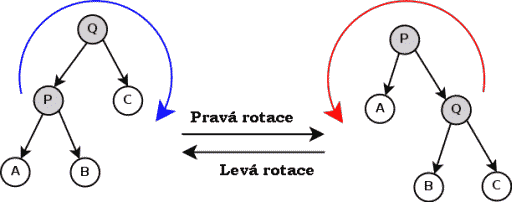
\includegraphics[width=12cm]{informatika/algoritmy_a_ds/obrazky/tree_rotation.png}

(Zdroj obrázku: Wikipedia)
\end{center}
\end{definiceN}


\begin{definiceN}{Červeno-černé stromy}
Červeno-černé stromy jsou binární vyhledávací stromy s garantovanou max. výškou $O(\log n)$, kde $n$ je počet uzlů, tj. operace na nich mohou mít asymptotickou časovou složitost $O(\log n)$. Pro jejich popis je nutné definovat \emph{interní uzly} - všechny uzly stromu a \emph{externí uzly} - na (interních) listech (a uzlech s jedním potomkem) uměle přidané NULLové ukazatele (de facto \uv{listy} červeno-černého stromu). Externí uzly slouží jenom jako abstrakce pro popis stromů, při implementaci se s nimi neoperuje. Červeno-černý strom má tyto čtyři povinné vlastnosti:
\begin{penumerate}
    \item Každý uzel (externí i interní) má definovanou barvu, a to černou nebo červenou.
    \item Každý externí uzel je černý.
    \item Každý červený vrchol musí mít oba syny černé.
    \item Každá cesta od libovolného vrcholu k listům v jeho podstromě musí obsahovat stejný počet černých uzlů.
\end{penumerate}

Pro červeno-černé stromy se definuje \emph{výška uzlu} $x$ ($\b{h}(x)$) jako počet uzlů na nedelší možné cestě k listu v jeho podstromě. \emph{Černá výška uzlu} ($\b{bh}(x)$) je počet černých uzlů na takové cestě.
\end{definiceN}

\begin{vetaN}{Vlastnosti červeno-černých stromů}
Podstrom libovolného uzlu $x$ obsahuje alespoň $2^{\b{bh}(x)}-1$ interních uzlů. Díky tomu má červeno-černý strom výšku vždy nejvýše $2\log(n+1)$ (kde $n$ je počet uzlů). (Důkaz prvního tvrzení indukcí podle $\b{h}(x)$, druhého z prvního a třetí vlastnosti červeno-černých stromů)
    \end{vetaN}

\begin{dusledek}
Operace hledání (minima, maxima, následníka, \dots), které jsou stejné jako u obecných binárních vyhledávacích stromů, mají garantovanou časovou složitost $O(\log n)$.
\end{dusledek}

\begin{algoritmusN}{Vkládání a odebírání uzlů v červeno černých stromech}
Obě operace mají podle garantované max. výšky garantovanou čas. složitost $O(\log n)$ pro $n$ počet uzlů. Protože bez porušení vlastností červeno-černých stromů lze kořen vždy přebarvit načerno, můžeme pro ně předpokládat, že \emph{kořen stromu} je \emph{vždy černý}.

\emph{Vkládání} vypadá následovně:
\begin{pitemize}
    \item Nalezení místa pro vložení a přidání nového prvku jako v obecných bin. vyhl. stromech, nový prvek se přebarví načerveno.
    \item Pokud je jeho otec černý, můžeme skončit -- vlastnosti stromů jsou splněné. Pokud je červený, musíme strom upravovat (tady předpokládám, že otec přidávaného uzlu je levým synem, opačný připad je symetrický):
    \item Je-li i strýc červený, přebarvit otce a strýce načerno a přenést chybu o patro výš (je-li děd černý, končím, jinak můžu pokračovat až do kořene, který už lze přebarvovat beztrestně).
    \item Je-li strýc černý a přidaný uzel je levým synem, udělat pravou rotaci na dědovi a přebarvit uzly tak, aby odpovídaly vlastnostem stromů.
    \item Je-li strýc černý a přidaný uzel je pravým synem, udělat levou rotaci na otci a převést tak na předchozí případ.
\end{pitemize}

\emph{Odebírání} se provádí takto:
\begin{pitemize}
    \item Odstraním uzel stejně jako v předchozím případě. Opravdu odstraněný uzel (z přepojování) má max. jednoho syna. Pokud odstraňovaný uzel byl červený, neporuším vlastnosti stromů, stejně tak pokud jeho syn byl červený -- to řeším jeho přebarvením načerno.
    \item V opačném případě (tj. syn odebíraného -- $x$ -- je černý) musím udělat násl. úpravy (přep. že $x$ je levým synem svého nového otce, v op. případě postupuji symetricky):
    \item $x$ prohlásím za \uv{dvojitě černý} a této vlastnosti se pokouším zbavit.
    \item Pokud je bratr $x$ (buď $w$) červený, pak má 2 černé syny -- provedu levou rotaci na rodiči $x$, prohodím barvy rodiče $x$ a uzlu $w$ a převedu tak situaci na jeden z násl. případů:
    \item Je-li $w$ černý a má-li 2 černé syny, prohlásím $x$ za černý a přebarvím $w$ načerveno, rodiče přebarvím buď na černo (a končím) nebo na \uv{dvojitě černou} a propaguji chybu (mohu dojít až do kořene, který lze přebarovat beztrestně).
    \item Je-li $w$ černý, jeho levý syn červený a pravý černý, vyměním barvy $w$ s jeho levým synem a na $w$ použiji pravou rotaci, čímž dostanu poslední případ:
    \item Je-li $w$ černý a jeho pravý syn červený, přebarvím pravého syna načerno, odstraním dvojitě černou z $x$, provedu levou rotaci na $w$ a pokud měl původně $w$ (a $x$) červeného otce, přebarvím $w$ načerveno a tohoto (teď už levého syna $w$) přebarvím načerno.
\end{pitemize}
\end{algoritmusN}


\begin{definiceN}{AVL stromy (Adelson-Velsky \& Landis)}
\emph{AVL stromy} jsou, podobně jako červeno-černé stromy, bin. vyhledávací stromy, které zaručují max. logaritmický nárůst výšky vzhledem k počtu prvků. Pro každý uzel $x$ se v AVL stromu definuje \emph{faktor vyvážení} jako rozdíl výšky jeho levého a pravého podstromu: $\b{bf}(x) = h(\texttt{x->levý}) - h(\texttt{x->pravý})$. Pro všechny uzly v AVL stromu platí, že $|\b{bf}(x)|\leq 1$.
\end{definiceN}

\begin{vetaN}{Zaručení výšky AVL stromů}
Výška AVL stromu s $n$ vrcholy je $O(\log n)$. (Důkaz: buď $T_n$ AVL strom výšky $n$ s minimálním počtem uzlů. Ten má podstromy $T_{n-1}$ a $T_{n-2}$ atd., tj. velikost minimálního AVL stromu roste jako Fibonacciho posloupnost, tedy $|T_n|\geq (\frac{1+\sqrt{5}}{2})^{n-1}$. Důkaz tohoto indukcí.)
\end{vetaN}

\begin{algoritmusN}{Operace na AVL stromech}
Vyhledávací operace se provádí stejně jako na obecných bin. vyhledávacích stromech, vkládání a odebírání prvků taky, ale pokud tyto operace poruší zákl. vlastnost AVL stromů ($|\b{bf}(x)=2|$), je nutné provést vyvažování -- pomocí rotací (které mohou být propagovány až ke kořeni). Při vkládání a odebírání je navíc nutné průběžně (nejhůře až ke kořeni) upravovat indikaci faktoru vyvážení jednotlivých uzlů.
\end{algoritmusN}

\subsubsection*{Halda}

\begin{definice}
\emph{Halda(heap)} je dynamická množina se stromovou strukturou (binární halda je binární strom), pro kterou platí tzv. \uv{vlastnost haldy}: $$\text{ Je-li }x\text{ potomek }y\text{, pak }x\texttt{->klíč}\geq y\texttt{->klíč}$$ Haldy s touto nerovností jsou tzv. \emph{min-heap}y, pokud je nerovnost opačná, jde o \emph{max-heap}.
\end{definice}

\begin{obecne}{(Binární) haldy}
Binární haldy jsou nejčastějším typem haldy. Zajišťují nalezení minimálního prvku v konstantním čase a odebrání a přidání minima v čase $O(\log n)$. V každé hladině od první až do předposlední je max. možný počet uzlů, v poslední jsou uzly co nejvíce \uv{vlevo} -- tedy max. výška haldy s $n$ prvky je $(\log n) + 1$. Proto je pro binární haldy jednoduše proveditelná jejich datová reprezentace polem (bez pointerů), kde při indexování od 0 má uzel na indexu $k$:
\begin{pitemize}
    \item Levého a pravého syna na indexu $2k+1$, resp. $2k+2$ (pokud to není víc než celk. počet prvků, potom syny nemá).
    \item Rodiče na indexu $\lceil\frac{k}{2}\rceil-1$. 
\end{pitemize}

\emph{Přidání uzlu} do haldy znamená přidání prvku na konec haldy a dokud má jeho rodič větší klíč, jeho prohazování s rodičem (tedy posouvání o vrstvu výš). Při \emph{odebírání uzlu} z haldy tento nahradím posledním prvkem v haldě a potom dokud neplatí vlastnost haldy (nejméně jeden z potomků má menší klíč), prohazuji ho s potomkem s menším klíčem (a posouvám o vrstvu níž).

Vytvoření haldy je možné v čase $O(n)$, kde $n$ je počet prvků v haldě -- přidání 1 prvku do haldy trvá $O(h)$, kde $h$ je aktuální výška (a $h$ roste od $0$ až k $\lceil\log n\rceil$, počet prvků ve výšce $k$ je $\frac{n}{2^{k+1}}$, bereme-li výšku listů rovnou nule) - v součtu za všechny prvky jde o $O(n\cdot\sum_{h=0}^{\lceil\log n\rceil}\frac{h}{2^h})$.

Binární halda se používá např. k \emph{třídění haldou} (heapsortu), kdy se z dat, která je potřeba utřídit, nejdříve postaví halda, a potom se opakuje operace odebrání kořene (tj. minimálního prvku).
\end{obecne}

\begin{obecne}{Fibonacciho haldy}
Fibonacciho haldy mají nízkou časovou složitost běžných operací -- amortizovaně $O(1)$ pro vložení, hledání minima apod.; odebrání prvku a odebrání minima má složitost $O(\log n)$ pro $n$ prvků v haldě. Tvoří ji skupina stromů, vyhovujících \uv{vlastnosti haldy}. Každý uzel haldy s $n$ prvky má max. $\log n$ potomků a ve svém podstromě minimálně $F_{k+2}$ uzlů, kde $F_k$ je $k$-té Fibonacciho číslo. To je zajištěno pravidlem, že při odebírání prvků lze z nekořenového uzlu oddělit max. 1 syna, jinak je nutné oddělit i tento uzel a ten se pak stane kořenem dalšího stromu. Počet stromů se snižuje při odebírání minima, kdy jsou spojovány dohromady.

Fibonacciho haldy se používají pro efektivní implementaci složitějších operací, jako např. Jarníkova nebo Dijkstrova algoritmu.
\end{obecne}

\newcommand{\nadpis}[1]{\pagebreak[2]\ramcek{\subsubsection*{#1}}}

\subsection{Hašování}

\begin{definiceN}{slovníkový problém} Dáno univerzum $U$, máme reprezentovat
$S \subseteq U$ a navrhnout algoritmy pro operace
\begin{pitemize}
\item MEMBER(x) - zjistí zda $x \in S$ a pokud ano nalezne kde,
\item INSERT(x) - pokud $x \notin S$, vloží $x$ do struktury reprezentující $S$,
\item DELETE(x) - když $x \in S$, smaže $x$ ze struktury reprezentující $S$.
\end{pitemize}
\end{definiceN}

Například pomocí pole můžeme tyto operace implementovat rychle, ale nevýhodou
je prostorová náročnost. Pro velké množiny je to někdy dokonce nemožné.
\emph{Hašování} se snaží zachovat rychlost operací a odstranit prostorovou
náročnost.

Podívejme se nyní na \emph{základní ideu} hašování. Mějme univerzum $U$ a
množinu $S \subseteq U$ takovou, že $|S| << |U|$. Dále mějme funkci
$h:U\rightarrow\{0,1,\dots,m-1\}$. Množinu $S$ potom reprezentujeme tabulkou
(polem) o velikosti $m$ tak, že prvek $x \in S$ je uložen na řádku $h(x)$.

\begin{definiceN}{Hašovací funkce, kolize} Funkci
$h:U\rightarrow\{0,1,\dots,m-1\}$ potom nazýváme \textbf{hašovací funkcí}.
Situaci $h(s)=h(t)$, pro $s \neq t; s,t \in S$  nazveme \textbf{kolize}.
\end{definiceN}

Jelikož mohutnost univerza $U$ je větší než velikost hašovací tabulky, nelze se
kolizím úplně vyhnout. Existuje spousta různých metod, jak kolize řešit.
Podívejme se tedy na některé podrobněji.

\begin{definice}
Ještě si zavedeme některé značení. Velikost $S$ (hašované množiny) označme
\textbf{n}, velikost tabulky (pole) označme \textbf{m}, a faktor naplnění
\textbf{$\alpha=\frac{n}{m}$}.
\end{definice}

\subsubsection*{Hašování se separovanými řetězci}

Použijeme pole velikosti $m$, jehož $i$-tá položka bude spojový seznam $S_i$
takový, že $s\in S_i \Leftrightarrow h(s)=i$, pro $s\in S$. Čili každý řádek
pole obsahuje spojový seznam všech (kolidujících) prvků, které jsou hašovány na
tento řádek. Seznamy nemusí být uspořádané, vznikají tak, jak jsou vkládány
jednotlivé prvky do struktury.

\begin{algoritmusN}{Hašování se separovanými řetězci}
\begin{pitemize}
\item \textbf{MEMBER} -- Spočteme hodnotu hašovací funkce $h(x)$, prohledáme
řetězec začínající na pozici $h(x)$ a zjistíme zda se prvek nachází, či
nenachází ve struktuře. Pokud se prvek v databázi nachází, tak musí nutně ležet
v tomto řetězci.
\item \textbf{INSERT} -- Zjistíme zda $x$ je v řetězci $h(x)$, pokud ne, přidáme
ho nakonec, v opačném případě neděláme nic.
\item \textbf{DELETE} -- Vyhledá $x$ v řetězci $h(x)$ a smaže ho. Pokud se tam
$x$ nenachází, neudělá nic.
\end{pitemize}
\end{algoritmusN}

\paragraph{Očekávaný počet testů} v neúspěšném případě je přibližně
$e^{-\alpha} + \alpha$ a při úspěšném vyhledávání přibližně
$1+\frac{\alpha}{2}$.

\subsubsection*{Hašování s uspořádanými řetězci}

Jak již je zřejmé z názvu je tato metoda téměř stejná jako předchozí. Jediný
rozdíl je, že jednotlivé seznamy jsou uspořádány vzestupně dle velikosti
prvků.

\begin{algoritmusN}{Hašování s uspořádanými řetězci}
Rozdíly jsou pouze pro operaci \textbf{MEMBER}, kde skončíme prohledávání, když
dojdeme na konec, nebo když nalezneme prvek, který je větší než hledaný a
operaci \textbf{INSERT}, které vkládá prvek na místo kde jsme ukončili
vyhledávání (před prvek, který ho ukončil).
\end{algoritmusN}

\paragraph{Očekávaný počet testů} v neúspěšném případě je přibližně roven
$e^{-\alpha}+1+\frac{\alpha}{2}-\frac{1}{\alpha}(1-e^{-\alpha})$ a v úspěšném
případě je přibližně $1+\frac{\alpha}{2}$.

Nevýhodou předchozích dvou metod je nerovnoměrné využití paměti. Zatímco
některé seznamy mohou být dlouhé, v některých není prvek žádný. Řešením je najít
způsob, jak kolidující prvky ukládat na jiné (prázdné) řádky tabulky. Potom je
ale nutné každý prvek tabulky rozšířit a položky pro práci s tabulkou. 

Čím použijeme sofistikovanější metodu ukládání dat do tabulky, tím více budeme
potřebovat položek pro práci s tabulkou a tedy vzroste paměťová náročnost. Naším
cílem je tedy najít rozumný kompromis mezi sofistikovaností (rychlostí)
strategie a její paměťovou náročností. Podívejme se na další algoritmy,
které se o to pokoušejí.

\subsubsection*{Hašování s přemísťováním}

Seznamy jsou tentokrát ukládány do tabulky a implementovány jako dvousměrné.
Potřebujeme tedy dvě položky pro práci s tabulkou: \emph{next} -- číslo řádku
obsahující další prvek seznamu a \emph{previous} -- číslo řádku obsahující
předchozí prvek seznamu. Když dojde ke kolizi, tj. chceme vložit prvek a jeho
místo je obsazené prvkem z jiného řetězce, pak tento prvek z jiného řetězce
přemístíme na jiný prázdný řádek v tabulce (proto hašování s přemísťováním).

\begin{algoritmusN}{Hašování s přemísťováním}
Algoritmus \textbf{MEMBER} funguje stejně jako u hašování se separovanými
řetězci, jen místo ukazatele na další prvek použije hodnotu \emph{next} z
tabulky. Při operaci \textbf{INSERT} vložíme prvek kam patří pokud je tam místo,
pokud již je místo obsazeno prvkem který tam patří, čili zde začíná seznam
kolidujících prvků (\emph{previous} = prázdné), pak postupujeme po položkách
\emph{next} až na konec seznamu, vložíme prvek na některý volný řádek
tabulky a vyplníme správně hodnoty \emph{next} a \emph{previous}. Pokud je místo
obsazeno prvkem z jiného seznamu (\emph{previous} $\neq$ prázdné), tak tento
prvek přemístíme na některý volný řádek, správně přepíšeme položky \emph{next} a
\emph{previous} v měněném seznamu a vkládaný prvek uložíme na jeho místo.
Operace \textbf{DELETE} je vcelku přímočará, jenom je třeba, pokud mažeme první
prvek seznamu na jeho místo přesunout ten druhý v pořadí (pokud existuje).
\end{algoritmusN}

\paragraph{Očekávaný počet testů} je v neúspěšném případě roven přibližně
$(1-\frac{1}{m})^n+\frac{n}{m}\approx e^{-\alpha}+\alpha$ a v úspěšném je stejný
jako pro hašování se separovanými řetězci a tedy $\frac{n-1}{2m}+1 \approx 1 +
\frac{1}{\alpha}$.

\subsubsection*{Hašování se dvěma ukazateli}

Hašování s přemísťováním má tu nevýhodu, že díky přemisťování prvků jsou operace
INSERT a DELETE časově náročné. Tato metoda tedy implementuje řetězce jako
jednosměrné seznamy, ale takové které nemusejí začínat na svém místě, tj.
řetězec $S_j$ obsahující prvky $s \in S$ takové, že $h(s)=j$, nemusí začínat na
$j$-tém řádku. Místo ukazatele na předchozí prvek tak do položek pro práci s
tabulkou přidáme ukazatel na místo, kde začíná řetězec příslušný danému řádku.
Položky pro práci s tabulkou tedy budou: \emph{next} -- číslo řádku tabulky kde
je další prvek seznamu, \emph{begin} -- číslo řádku tabulky obsahující první
prvek seznamu příslušného tomuto místu.

\begin{algoritmusN}{Hašování se dvěma ukazateli}
Položka \emph{begin} v $j$-tém řádku je vyplněna právě tehdy, když
reprezentovaná množina $S$ obsahuje prvek $s \in S$ takový, že $h(s)=j$.
Algoritmy jsou potom podobné těm u hašování s přemísťováním, ale přemísťování
prvků je nahrazeno odpovídajícími změnami v položce \emph{begin} daných řádků.
\end{algoritmusN}

Díky práci s položkami jsou operace INSERT a DELETE rychlejší než při hašování s
přemísťováním, ale začátek řetězce v jiném řádku tabulky přidá navíc jeden test,
což změní složitost operace MEMBER.

\paragraph{Očekávaný počet testů} v neúspěšném případě je přibližně
$1+\frac{\alpha^2}{2}+\alpha+e^{-\alpha}(2+\alpha)-2$ a při úspěšném vyhledávání
je roven $1+\frac{(n-1)(n-2)}{6m^2}+\frac{n-1}{2m} \approx 1 +
\frac{\alpha^2}{6}+\frac{\alpha}{2}$

\subsubsection*{Srůstající hašování}

Nyní se podíváme na několik verzí metody, která se nazývá srůstající hašování.
Budeme potřebovat jedinou položku pro práci s tabulkou a to ukazatel
jednosměrného spojového seznamu. Na rozdíl od předchozích metod zde nejsou
řetězce separované, v jednom řetězci mohou být prvky s různou hodnotou hašovací
funkce. Když máme přidat prvek $s$, tak ho zařadíme do řetězce, který se nachází
na $h(s)$-tém řádku tabulky. Řetězce tedy v této metodě \emph{srůstají}. Různé
verze této metody se liší tím, kam přidáváme nový prvek a podle práce s pamětí.
Dělí se na \emph{standardní srůstající hašování} bez pomocné paměti a na hašování
používající pomocnou paměť, kterému se říká jen \emph{srůstající hašování}.

Nejdříve se budeme věnovat metodám standardního srůstajícího hašování (bez
pomocné paměti):
\begin{pitemize}
\item \textbf{LISCH} -- late-insertion standard coalesced hashing -- vkládá se
za poslední prvek řetězce,
\item \textbf{EISCH} -- early-insertion standard coalesced hashing -- vkládá se
za první prvek řetězce.
\end{pitemize}

Přirozená efektivní operace DELETE pro standardní srůstající hašování není
známa. Na druhou stranu i primitivní algoritmy mají rozumnou očekávanou časovou
složitost.

Další otázka zní, proč používat metodu EISCH, když programy pro metodu LISCH
jsou jednodušší. Odpověď je na první pohled dost překvapující. Při úspěšném
vyhledávání je metoda EISCH rychlejší než metoda LISCH. Je to proto, že je o
něco pravděpodobnější, že se bude pracovat s novým prvkem. V neúspěšném případě
jsou samozřejmě obě metody stejné, neboť řetězce jsou u obou stejně dlouhé.

Metody srůstajícího hašování (s pomocnou pamětí) mají použitou paměť rozdělenou
na dvě části. Na tu přímo adresovatelnou hašovací funkcí a na pomocnou část.
Adresovací část má $m$ řádků, pokud hašovací funkce má hodnoty z oboru
$\{0,1,\dots,m-1\}$, v pomocné části jsou řádky ke kterým nemáme přístup přes
hašovací funkci. Když při přidávání nového prvku vznikne kolize, tak se nejprve
vybere volný řádek z pomocné části a teprve když je pomocné část zaplněna
použijí se k ukládání kolidujících prvků řádky z adresovatelné části tabulky.
Tato strategie oddaluje srůstání řetězců. Srůstající hašování se tedy, aspoň
dokud není zaplněna pomocná část tabulky, podobá hašování se separovanými
řetězci. Existují základní tři varianty:
\begin{pitemize}
\item \textbf{LICH} -- late-insertion coalesced hashing -- vkládá prvek na konec
řetězce,
\item \textbf{VICH} -- early-insertion coalesced hashing -- vkládá prvek na
řádek $h(x)$ pokud je prázdný a nebo hned za prvek na řádku $h(x)$,
\item \textbf{EICH} -- varied-insertion coalesced hashing -- vkládá se za
poslední prvek řetězce, který je ještě v pomocné části. Pokud v pomocné části
žádný není, vkládá se hned za prvek na pozici $h(x)$.
\end{pitemize}

Tyto metody nepodporují přirozené efektivní algoritmy pro operaci DELETE.

\subsubsection*{Hašování s lineárním přidáváním}

Následující metoda nepoužívá žádné položky pro práci s tabulkou to znamená, že
způsob nalezení dalšího řádku řetězce je zabudován přímo do metody. Metoda
funguje tak, že pokud chceme vložit prvek do tabulky a nastane kolize, najdeme
první následující volný řádek a tam prvek vložíme. Předpokládáme, že řádky jsou
číslovány modulo \emph{m}, čili vytvářejí cyklus délky \emph{m}.

Tato metoda sice využívá minimální velikost paměti, ale v tabulce vznikají
shluky obsazených řádků a proto je při velkém zaplnění pomalá. Navíc metoda
nepodporuje efektivní operaci DELETE.

\subsubsection*{Shrnutí}

Zde uvedeme pořadí metod hašování podle očekávaného počtu testů.

\begin{obecne}{Neúspěšné vyhledávání:}
\begin{penumerate}
\item Hašování s uspořádanými separovanými řetězci,
\item Hašování se separovanými řetězci = Hašování s přemísťováním,
\item Hašování se dvěma ukazateli,
\item VICH = LICH
\item EICH,
\item LISCH = EISCH,
\item Hašování s lineárním přidáváním.
\end{penumerate}
\end{obecne}

\begin{obecne}{Úspěšné vyhledávání}
\begin{penumerate}
\item H. s uspořádanými řetězci = H. se separovanými řetězci = H. s přemísťováním,
\item Hašování se dvěma ukazateli,
\item VICH,
\item LICH,
\item EICH,
\item EISCH,
\item LISCH,
\item Hašování s lineárním přidáváním.
\end{penumerate}
\end{obecne}

\begin{poznamka} Metody se separovanými řetězci a srůstající hašování používají
více paměti. Metoda s přemísťováním vyžaduje více času -- na přemístění prvku.
Otázka která z metod je nejlepší není proto jednoznačně rozhodnutelná a je nutné
pečlivě zvážit všechny okolnosti nasazení metody a všechny naše požadavky na ní,
než se rozhodneme, kterou použijeme.
\end{poznamka}

\subsubsection*{Univerzální hašování}

Pro dobré fungování hašování potřebujeme mimo jiné, aby vstupní data byla
rovnoměrně rozdělena a toho někdy není možné dosáhnout. Odstranit tento
nedostatek se pokouší metoda \emph{univerzální hašování}. Základní idea této
metody je taková, že máme množinu \emph{H} hašovacích funkcí z univerza do
tabulky velikosti \emph{m} takových, že pro $S \subseteq U$, $|S| \leq m$ se
většina funkcí chová dobře v tom smyslu, že má malý počet kolizí. Hašovací
funkci potom zvolíme z množiny \emph{H} (takovou s rovnoměrným rozdělením).
Jelikož funkci volíme my, můžeme požadavek rovnoměrného rozdělení zajistit.

\subsubsection*{Perfektní hašování}

Jiná možnost jak vyřešit kolize, je najít takzvanou \emph{perfektní hašovací
funkci}, tj. takovou které nepřipouští kolize. Nevýhoda této metody je, že nelze
dost dobře implementovat operaci INSERT, proto se dá prakticky použít pouze tam,
kde předpokládáme hodně operací MEMBER a jen velmi málo operací INSERT. Kolize
se potom dají řešit třeba malou pomocnou tabulkou, kam se ukládají kolidující
data. 

Pro rozumné fungování metody je nutné, aby hašovací funkce byla rychle
spočitatelná a aby její zadání nevyžadovat mnoho paměti, nejvýhodnější je
analytické zadání. 

Naopak jedna z výhod je, že nalezení perfektní hašovací funkce, může trvat
dlouho, neboť ho provádíme pouze jednou na začátku algoritmu. 

\subsubsection*{Externí hašování}

Externí hašování řeší trochu jiný problém, než výše popsané metody. Chceme
uložit data na externí médium a protože přístup k externím médiím je o několik
řádů pomalejší, než práce v interní paměti, bude naším cílem minimalizovat počet
přístupů do ní. Externí paměť bývá rozdělena na stránky a ty většinou načítáme
do interní paměti celé. Tato operace je však velice pomalá. Problémem externího
hašování je tedy nalézt datovou strukturu pro uložení dat na vnější paměti a
algoritmy pro operace INSERT, DELETE a MEMBER, tak abychom použili co nejmenší
počet komunikací mezi vnější a vnitřní pamětí.

Metod externího hašování je opět mnoho. Některé používají pomocnou datovou
strukturu v interní paměti, kterou často nazýváme adresář. Pokud metody nemají
žádnou takovou pomocnou strukturu neobejdou se obvykle bez oblasti přetečení.
Některé známější metody vnějšího hašování jsou například: \uv{Litwinovo lineární
hašování}, \uv{Faginovo rozšiřitelné hašování}, \uv{Cormackovo perfektní
hašování} nebo \uv{Perfektní hašování Larsona a Kajli}. 
% to neni preklep, hasovani je opravdu od pana KAJLI z nakyho duvodu se to uci
% blbe. viz http://portal.acm.org/citation.cfm?id=358193&coll=portal&dl=ACM
% ajs

\subsection{Sekvenční třídění, porovnávací algoritmy, přihrádkové třídění, třídící sítě}

TODO: trochu víc formalismu by tu neškodilo, taky je potřeba sjednotit óčkovou notaci (zřejmě prosté nahrazení symbolu $O$ symbolem $\Theta$ by stačilo, ale chce to ověřit).

\subsubsection*{Sekvenční třídění a porovnávací algoritmy}

Pojmy \uv{sekvenční třídění} a \uv{porovnávací algoritmy} mohou znamenat vlastně cokoliv, takže uvedu pár nejběžnějších třídících algoritmů a budu doufat, že to bude ke zkoušce stačit \texttt{:-(}. Zdrojem mi budiž Wikipedie a kniha Algoritmy a programovací techniky Doc. P. Töpfera.

\bigskip

\begin{algoritmusN}{Selection sort, třídění výběrem}
Selection sort je jeden z nejjednodušších třídích algoritmů. Jde o vnitřní třídění -- tedy celá posloupnost prvků by měla být v paměti. Má časovou složitost $\Theta(n^2)$ a obecně bývá pomalejší než insertion sort. Pracuje následovně:

Udržuje si množinu setříděných prvků na začátku posloupnosti (pole), která je na začátku prázdná a na konci představuje celé pole. Zbytek pole za setříděnou množinou je neuspořádaný. V jednom kroku vždy vybere jeden prvek a vloží ho do utříděné části (kterou tím zvětší o 1 a zároveň zmenší nesetříděnou). Jeden krok algoritmu (kterých je $n$ pro $n$ prvků v každém případě) vypadá takto: 
\begin{penumerate}
    \item Najdi nejmenší prvek z nesetříděného úseku.
    \item Vlož ho přesně za konec setříděného úseku (a prvek co tam byl původně si s ním vymění místo)
\end{penumerate}

Heapsort, který popíšu později, může být považovaný za variantu selection sortu, protože také vybírá minimum a začleňuje do setříděné části.
\end{algoritmusN}

\begin{algoritmusN}{Insertion sort, třídění vkládáním}
Insertion sort je také relativně jednoduchý a na velké datové soubory neefektivní, ale jednoduchý na implementaci a rychlejší než nejprimitivnější algoritmy bubble sort a selection sort. Navíc je efektivní pro data, která jsou už částečně předtříděná -- v nejhorším případě sice běží v čase $O(n^2)$, ale v nejlepším případě (úplné setřídění dat) je lineární -- obecně běží v čase $O(n+d)$, kde $d$ je počet inverzí ve tříděné posloupnosti. Navíc je stabilní (zachovává pořadí prvků se stejným klíčem) a \uv{in-place}, tedy nepotřebuje žádné pomocné datové struktury. Proti selection sortu ale většinou potřebuje více přepisování (a to může u velkých datových struktur vadit).

V jednom kroku vždy vezme nějaký prvek (berou se po řadě od začátku pole), zapamatuje si jeho hodnotu, a dokud před ním jsou prvky s větším klíčem, posouvá je na pozici o 1 větší (čímž vždy přepíše následující, takže původní prvek se ztratí) a pokud narazí na prvek s menším klíčem, do za něj napíše onen zapamatovaný prvek (a místo tam je, protože celou cestu k němu posouval prvky). Algoritmus vypadá takto:
\begin{verbatim}
insert sort( array a ){
  for( i = 1; i < a.length - 1; ++i ){
    value = a[i];
    j = i-1;
    while( j >= 0 && a[j] > value ){ 
      a[j + 1] = a[j];
      j = j-1;
    }
    a[j+1] = value;
  }
}
\end{verbatim}

Jednou z variant insertion sortu je \emph{Shell sort}, který porovnává prvky ne vedle sebe, ale vzdálené o nějaký počet polí, který se postupně zmenšuje. Může dosahovat složitost $O(n^{3/2})$ až $O(n^{4/3})$. S jistými úpravami se u něj dá dosáhnout až $O(n\log^2 n)$. Jiné vylepšení je \emph{library sort}, který si při vkládání nechává mezery pro další prvky (podobně jako v knihovně nejsou poličky úplně plné) -- ten může s velkou pravděpodobností běžet v čase $O(n\log n)$, ale zase potřebuje větší paměťový prostor.
\end{algoritmusN}

\begin{algoritmusN}{Bubble sort, bublinkové třídění}
Bubble sort je velmi jednoduchý třídící algoritmus (asi nejjednodušší na implementaci), s časovou složitostí $O(n^2)$. V nejlepším případě (pro úplně setříděná data) mu ale stačí jen jeden průchod, takže $O(n)$. Většinou ale bývá pomalejší i než insertion sort, takže se na velké množiny dat nehodí.

Algoritmus prochází v jednom kroku celé pole a hledá pozice, kde se prvek s menším klíčem nachází bezprostředně za prvkem s větším klíčem. Takovéto dva prvky pak vymění. Kroky opakuje, dokud neprojde celé pole bez jediného prohození prvků (nebo v \uv{tupější} variantě $n$-krát pro $n$ prvků, protože pak je zaručeno, že posloupnost bude pro libovolné pořadí prvků setříděná -- ta má ale pak složitost $O(n^2)$ v každém případě!).

Vylepšení algoritmu lze dosáhnout jednoduchou úvahou: největší prvek je už při prvním průchodu polem odsunutý až na konec. To se samozřejmě opakuje pro každý průchod (ve druhém je předposlední na druhém místě od konce atp.), takže lze průchody postupně zkracovat a konec pole už netestovat -- dosáhneme tím v průměru dvojnásobné rychlosti.

Variantou bubble sortu je \emph{shake sort} neboli \emph{cocktail sort}, který střídavě prochází posloupnost prvků nejdřív od začátku a pak od konce (a přitom provádí to samé jako bubble sort). Tím může v některých případech o trochu třídění zrychlit -- příkladem budiž posloupnost prvků $(2,3,4,5,1)$, která potřebuje jen 1 průchod cocktail-sortem tam a jeden zpět, ale pro bubble-sort by potřebovala 4.

Dalším vylepšením bubble sortu je \emph{Comb sort}, který o něco zvyšuje rychlost. Je založen na stejné myšlence jako shell sort -- tedy nejsou porovnávány prvky bezprostředně za sebou, ale prvky posunuté o nějaký ofset -- ten je na začátku roven délce posloupnosti, a postupně se dělí \uv{zkracovacím faktorem} (běžná hodnota $1.3$) až dosáhne jedné. Složitost se pohybuje mezi $O(n^2)$ v nejhorším případě a $O(n\log n)$ v nejlepším. V průměrném případě jde stále o $O(n^2)$, ale s menší konstantou než u bubble-sortu (TODO: tohle je potřeba set-sakra ověřit ... opsané z německé wiki a \uv{talk:Comb sort} na anglické, takže fakt \uv{důvěryhodné}).
\end{algoritmusN}

\begin{algoritmusN}{Heap sort, třídění haldou}
Heapsort je také třídící algoritmus založený na porovnávání a myšlenkově vychází ze selection sortu, ke kterému přidává práci s haldou. Většinou bývá pro typická vstupní data pomalejší než quicksort, ale zaručuje časovou složitost $O(n\log n)$ i v nejhorším případě. Jde o \uv{in-place} algoritmus (halda se může nacházet přímo v nesetříděné části pole), ale není \uv{stabilní}.

Algoritmus sám, máme-li vyřešené operace na haldě, je velice jednoduchý -- nejdříve pro každý prvek opakuje jeho vložení do haldy (takže postupně vytvoří $n$-prvkovou haldu, která se s každým krokem zvětšuje o 1), pro implementaci haldy na začátku pole je vhodný \uv{max-heap}, a potom opakuje odebrání maxima a jeho přesun na volné místo hned za konci zmenšivší se haldy -- takže od konce pole postupně roste směrem k začátku setříděná posloupnost.

Upravený heapsort s použitím ternární haldy dosahuje o multiplikativní konstantu lepší výsledky, existuje i (prý :-)) složitá varianta \emph{smoothsort}, která se blíží časové složitosti $O(n)$, pokud jsou data částečně předtříděná -- heapsort totiž pracuje pro libovolnou posloupnost v čase $O(n\log n)$.
\end{algoritmusN}

\begin{algoritmusN}{Merge sort, třídění sléváním}
Dalším třídícím algoritmem založeným na porovnávání prvků je mergesort. Je stabilní, takže zachovává pořadí dat se stejným klíčem. Jde o příklad algoritmu typu \uv{rozděl a panuj}, stejně jako u níže popsaného quicksortu. Byl vynalezen Johnem Von Neumannem. Je založen na rozdělení posloupnosti na dvě zhruba stejné poloviny, rekurzivním setřídění a potom \uv{slévání} dvou již setříděných posloupností. Jeho časová složitost je $O(n\log n)$ i v nejhorším případě, provádí většinou méně porovnání než quicksort, má větší nároky na paměť v případě rekurzivního volání (existuje ale i nerekurzivní verze), ale většinou nepracuje na místě a potřebuje alokovat paměť pro výstup setříděných posloupností (i toto se dá odstranit, ale je to zbytečně složité a přílišné zrychlení oproti použití jiného algoritmu nepřinese). Jeho přístup ho ale činí ideálním k použití na médiích se sekvenčním přístupem k datům (např. pásky). Jde tedy použít i ke třídění na vnější paměti -- detaily viz sekce o databázích.

Postup práce je následující:
\begin{penumerate}
    \item Rozděl nesetříděnou posloupnost na dvě (zhruba) poloviční části    
    \item Pokud mají více než jeden prvek, setřiď je rekurzivním zavoláním mergesortu (tj. pro každou z nich pokračuj od kroku 1 do konce algoritmu), jinak pokračuj následujícím krokem.
    \item Slij dvě setříděné posloupnosti do jedné -- vyber z obou posloupností první prvek, a pak opakovaně prvky porovnávej, zapisuj do setříděné posloupnosti menší z nich a doplňuj dvojici z té poloviční posloupnosti, odkud pocházel zapsaný prvek.
\end{penumerate}
\end{algoritmusN}

\begin{algoritmusN}{Quicksort}
Quicksort je jedním z nejrychlejších algoritmů pro třídění na vnitřní paměti, přestože v nejhorším případě může jeho časová složitost dosáhnout až $\Theta(n^2)$. Pro ideální i průměrná data dosahuje $\Theta(n\log n)$. Je také založen na principu \uv{rozděl a panuj}, i když poněkud jiným způsobem než předchozí zmiňovaný, od něhož se liší i tím, že není stabilní.

Algoritmus nejdřív vybere nějaký prvek, tzv. \emph{pivot}, a prvky s klíčem větší než pivot přesune do jiné části pole než ty s klíčem menším. Pak rekurzivně třídí obě části pole -- když se dostane k polím délky 1, problém je vyřešen. Postup vypadá takto:
\begin{penumerate}
    \item Vyber pivot (jeden prvek ze seznamu). Tady jde o největší magii, protože k dosažení nejlepší rychlosti by se měl pokaždé vybírat medián. Nejjednodušší je vybrat první, ale tento výběr ovlivňuje výslednou rychlost práce, takže se vyplatí např vzít tři prvky, porovnat je a vzít si z nich ten prostřední.
    \item Postupuj od začátku pole a hledej první prvek větší nebo rovný než pivot. Až ho najdeš, postupuj od konce a najdi první prvek menší než pivot. 
    \item Prvky prohoď a opakuj krok 2 a 3, dokud se hledání od začátku a od konce nepotká na nějaké pozici -- tu pojmenujeme třeba $k$.
    \item Rekurzivním voláním setřiď prvky $(0,\dots,k)$ a $(k+1,\dots,n-1)$ (má-li tříděné pole délku $n$) -- to znamená pro obě části pole pokračuj od kroku 1. Pokud je $k=0$ nebo $k=n-2$, není třeba už rekurzivního volání, protože posloupnosti délky 1 jsou setříděné.
\end{penumerate}

Pro algoritmus existuje i nerekurzivní verze (stačí rekurzi nahradit zásobníkem úseků čekajících na zpracování). Je vidět, že na volbě pivotu závisí všechno -- pokud pokaždé jako pivot volím 1. nebo $n-1$. hodnotu v poli v pořadí podle velikosti, dělím pak vždy na části o délce 1 a $n-1$, takže tento rekurzivní krok provedu až $n$-krát a dostanu se k času $\Theta(n^2)$. Samozřejmě, díky existenci algoritmu pro nalezení mediánu v čase $\Theta(n)$ je možné i tady dosáhnout zaručené složitosti $\Theta(n\log n)$, ale v praxi je to kvůli vysoké multiplikativní konstantě nepoužitelné -- k výběru pivotu se většinou s úspěchem užívá nějaká jednoduchá heuristika, jak je nastíněno v popisu algoritmu samotného.

Heapsort bývá pomalejší než quicksort, ale zaručuje nízkou časovou složitost i pro nejhorší případ a navíc potřebuje méně paměti -- nároky quicksortu navíc (kromě tříděné posloupnosti) jsou $O(\log n)$ minimálně, kvůli nutnosti použití rekurzivního volání nebo zásobníku. Oproti mergesortu ho nelze použít na data se sekvenčním přístupem, tyto nevýhody ale vyvažuje relativní jednoduchostí implementace a rychlostí v průměrném případě.

Variantou quicksortu je \emph{introsort}, který ho kombinuje s heapsortem, pokud hloubka rekurze dosáhne nějakých nepřijatelných hodnot -- tak je zaručena časová složitost $\Theta(n\log n)$ i v nejhorším případě (samozřejmě je to ale v nejhorším případě pořád pomalejší než použití jen heapsortu). Jedna z variant tohoto algoritmu se dá použít k hledání $k$-tého nejmenšího prvku (tedy i mediánu), kdy dosahuje složitosti $O(n)$ průměrně až $O(n^2)$ nejhůře.
\end{algoritmusN}


\subsubsection*{Přihrádkové třídění}

\begin{algoritmusN}{Bucket sort, Radix sort, přihrádkové třídění}
Radix sort je zvláštní třídící algoritmus -- jeho složitost je totiž lineární. Dosahuje to tím, že neporovnává všechny tříděné prvky (složitost problému třídění pomocí porovnávání je $\Theta(n\log n)$, takže by to jinak nebylo možné), je ho ale možné použít jen pro třídění dat podle klíče z nějaké ne příliš velké množiny -- max. rozsah tříděných hodnot závisí na tom, jak velké pole si můžeme dovolit vymezit v paměti pro tento účel.

Nejjednodušší varianta (tzv. \emph{pigeonhole sort}, nebo-li \emph{counting sort}) opravdu počítá s klíči ze zadaného rozmezí $[l,h]$. Pro něj si připraví cílové pole velikosti $h-l+1$, tj. \uv{přihrádky}. Do nich pak přímo podle klíče přehazuje čtené prvky (jestliže přihrádky realizujeme jako seznamy, bude třídění dokonce stabilní). Nakonec projde přihrádky od začátku do konce a co v nich najde, to vypíše (a výstup bude setříděný). Variantou counting sortu je \emph{bucket sort}, kdy se do jedné přihrádky nedávají jen prvky se stejným klíčem, ale prvky s klíčem v nějakém malém rozmezí -- ty pak lze setřídit rychle, protože jich zřejmě nebude mnoho, a navíc se ušetří paměť.


Protože ale klíče velikosti max. tisíců hodnot jsou většinou trochu málo, v praxi se běžně používají složitější varianty -- ty zahrnují několik průchodů nahoře popsaného algoritmu, při nichž se třídí jenom podle části klíče. Ty se dělí na ty, které začínají od nejméně významné části klíče (\emph{least significant digit radix sort}) a ty, které jdou od nejvýznamnější části (\emph{most significant digit}). První z nich mají tu výhodu, že lze zachovat stabilitu třídění, druhá zase může třídit i podle klíčů různé délky a zastavovat se po nalezení unikátních prefixů, takže se hodí např. pro lexikografické třídění podle řetězcových klíčů.

Třídění typu least significant digit vypadá následovně:
\begin{penumerate}
    \item Vezmi nejméně významnou část klíče (určitý počet bitů).
    \item Rozděl podle této části klíče data do přihrádek, ale v nich zachovej jejich pořadí (to je nutné kvůli následnému průchodu, zároveň to dělá z tohoto algoritmu stabilní třídění).
    \item Opakuj toto pro další (významnější) část klíče.
\end{penumerate}

Most significant digit varianta (rekurzivní verze, je založená na bucket sortu) běhá takto:
\begin{penumerate}
    \item Vezmi nejvýznamnější část klíče (první písmeno, například).
    \item Rozděl prvky podle této části do přihrádek (takže v jedné se jich octne docela hodně)
    \item Rekurzivně setřiď každou z přihrádek (začni podle další části klíče), pokud je v ní více než jeden prvek (tohle zaručí zastavení za rozlišujícím prefixem).
    \item Slep přihrádky do jedné (setříděné) posloupnosti.
\end{penumerate}

Popisované algoritmy většinou potřebují $O(n+(h-l))$ času k třídění, je-li $h-l$ (zhruba) počet přihrádek -- to znamená, že sice jde o složitost lineární, ale lineární i v počtu přihrádek, což se nemusí vždy oproti konvenčnímu třídění vyplatit. Navíc jsou problémem vysoké nároky na paměť (nelze třídění provést \uv{na místě} v jediném poli). Pro malou množinu hodnot klíčů (nebo u most significant digit varianty krátké odlišující prefixy) jsou ale časově efektivnější.
\end{algoritmusN}



\subsubsection*{Třídící sítě}

Zdrojem této sekce jsou zápisky z přednášek Prof. L. Kučery Algoritmy a datové struktury II.
\bigskip

\begin{definiceN}{Bitonická posloupnost}
Řekneme, že posloupnost prvků je \emph{bitonická}, pokud po spojení do cyklu (tedy nultý prvek za $n$-tý) obsahuje dva monotónní úseky. Nebo-li obsahuje až na fázový posuv dva monotónní úseky.
\end{definiceN}

\begin{definiceN}{Komparátor}
\emph{Komparátor} je speciální typ hradla (představme si pod tím nedělitelnou elektronickou součástku, případně jen virtuální), která má dva výstupy a dva vstupy. Pokud na vstupy přivedeme dva prvky (klíče, čísla), z levého výstupu vydá menší z nich a z pravého výstupu větší (takže vlastně porovná dva prvky a na výstup je vyplivne ve správném pořadí). Pracuje v konstantním čase.
\end{definiceN}

\begin{definiceN}{Třídící síť}
Třídící síť je správně sestavená množina komparátorů dohromady spojená vstupy a výstupy tak, že při přivedení posloupnosti délky $n$ na vstup ji vydá setříděnou na výstupu. Komparátory v ní jsou rozčleněné do hladin, jejichž počet pak udává celkovou dobu výpočtu -- předpokládá se tam, že komparátory v jednotlivých vrstvách pracují paralelně, takže třídící sítě mohou dosahovat časové složitosti pouhých $O(\log n)$. Algoritmus s takovou časovou složitostí sice existuje, ale má velmi vysokou multiplikativní konstantu, takže se v praxi nepoužívá. Příkladem třídící sítě je i bitonické třídění.
\end{definiceN}

\begin{algoritmusN}{Bitonické třídění}
Bitonická třídící síť je založena na použití bitonických posloupností a rekurze. Obvod (pro třídění dat délky $n$) se dělí na dvě části:
\begin{pitemize}
    \item První část setřídí (rekurzivně) $1/2$ vstupu vzestupně, druhou polovinu sestupně a tím vytvoří bitonickou posloupnost. Obsahuje tedy dvě třídící sítě pro třídění posloupností délky $\frac{n}{2}$.
    \item Druhá část třídí jen bitonické posloupnosti -- první její vrstva rozdělí bitonickou posloupnost na vstupu na dvě bitonické posloupnosti (z větších a menších čísel). Další vrstvy už jsou opět implementovány rekurzivně -- tedy druhá vrstva dostane dvě posloupnosti a vyrobí z nich čtyři atd., až nakonec dojde k \uv{bitonickým posloupnostem} délky 1.
\end{pitemize}

K rozdělení jedné bitonické posloupnosti délky $k$ na dvě stačí jen $\frac{k}{2}$ komparátorů, které porovnávají vždy $i$-tý a $k+i$-tý prvek. Dojde sice k nějakému fázovému posuvu, ale to ničemu nevadí. Dobře je to vidět při znázornění na kružnici, doporučuji prohlédnout si postup v programu Algovision Prof. Kučery (\texttt{http://kam.mff.cuni.cz/\~{}ludek/AlgovisionPage.html}).

Je vidět, že počet vrstev potřebných k dělení bitonických posloupností délky $N$ je $log_2 N$ ($B(N)=\log N$). Pro celkový počet vrstev, a tedy dobu zpracování -- $T(n)$ nám vychází následující vzorec
$$T(N) = T(\frac{n}{2}) + B(N) = \log N + \log(N/2) + \dots + 1$$
z čehož díky vzorci pro součet aritmetické posloupnosti $1+2+\dots+k=\frac{k(k+1)}{2}$ vyjde
$$T(N) = O(\frac{1}{2} \log^2 N)$$
\end{algoritmusN}

\def\Real{ \mathbb{R} }

\subsection{Grafové algoritmy}

TODO: nejake vyuziti tech algoritmu (staci priklad plusminus ke kazdemu druhu ulohy)

\subsubsection*{Graf}

\begin{definice}
\emph{Graf} $G$ je dvojice $(V,E)$, kde $V$ je množina bodů (\emph{vrcholů}) a $E$ množina jejich dvojic (\emph{hran}). Je-li $E$ množinou neuspořadaných dvojic, jde o \emph{neorientovaný} graf. Jsou-li dvojice uspořádané, jedná se o \emph{orientovaný} graf. Velikost množiny $V$ se značí $n$, velikost $E$ je $m$ - $|V|=n$, $|E|=m$. 

Graf je možné strojově reprezentovat např. pomocí \emph{matice sousednosti} -- matice, kde je na souřadnicích $(u,v)$ hodnota $1$, pokud z $u$ do $v$ je hrana a $0$ jinak. Pro neorientované grafy je souměrná podle hlavní osy. Matice zabírá $\Theta(n^2)$ místa v paměti. Další možností jsou \emph{seznamy sousedů} -- dvě pole, jedno příslušné vrcholům, druhé hranám. V prvním jsou uložené indexy do druhého pole, určující kde začínají seznamy hran vedoucích z vrcholu (příslušejícímu k indexu v prvním poli). Paměťová náročnost je $\Theta(m+n)$.
\end{definice}

\subsubsection*{Prohledávání do hloubky a do šířky}

Algoritmy, které postupně projdou všechny vrcholy daného souvislého neorientovaného grafu.

\begin{algoritmusN}{Prohledávání do šířky/Breadth-First Search}
Prochází všechny vrcholy grafu postupně po vrstvách vzdáleností od iniciálního vrcholu. K implementaci se používá fronta (FIFO).

\begin{verbatim}
BFS( V - vrcholy, E - hrany, s - startovací vrchol ){
  obarvi vrcholy bíle, nastav jim nekonečnou vzdálenost od s a předchůdce NULL;
  dej do fronty vrchol s;

  while( neprázdná fronta ){
    vyber z fronty vrchol v;
    foreach( všechny bíle obarvené sousedy v = u ){
       obarvi u šedě a nastav mu vzdálenost d(v) + 1 a předchůdce v;
       dej vrchol u do fronty;
    }
    v přebarvi na černo a vyhoď z fronty.
  }
}
\end{verbatim}


Běží v čase $\Theta(m+n)$, protože každý vrchol testuje 2x pro každou hranu, do fronty ho dává 1x a obarvení mu mění 2x. Tento algoritmus je základem několika dalších, např. pro testování souvislosti grafu, hledání minimální kostry nebo nejkratší cesty.
\end{algoritmusN}

\begin{algoritmusN}{Prohledávání do hloubky/Depth-First Search}
Prochází postupně všechny vrcholy - do hloubky (pro každý vrchol nejdřív navštíví první jeho nenavštívený    sousední vrchol, pak první sousední tohoto vrcholu atp. až dojde k vrcholu bez nenavštívených sousedů, pak se vrací a prochází další ještě nenavštívené sousedy). Pro implementaci se používá buď zásobník, nebo rekurze. Zásobníková verze vypadá stejně jako prohledávání do šířky (místo fronty je zásobník).

Rekurzivní verze - při zavolání na startovní vrchol projde celý graf:
\begin{verbatim}
DFS(v - vrchol){

  označ v jako navštívený;
  foreach( všechny nenavštívené sousedy v = u )
     DFS( u );
}
\end{verbatim}

Časová složitost je $\Theta(m+n)$, stejně jako u prohledávání do šířky.
\end{algoritmusN}


\subsubsection*{Souvislost}

\begin{definice}
\emph{Cesta} v grafu $G=(V,E)$ z vrcholu $a$ do vrcholu $b$ je posloupnost $v_0,v_1,\dots,v_n$ taková, že $v_0=a$, $v_n=b$ a pro všechna $v_i$, $i\in\{1,\dots,n\}$ je $(v_{i-1},v_i)\in E$. Graf $G=(V,E)$ je \emph{souvislý}, pokud pro každé dva vrcholy $u,v\in V$ existuje v $G$ cesta z $u$ do $v$. Toto platí pro orientované i neorientované grafy.
\end{definice}

\begin{algoritmusN}{Testování souvislosti grafu/počítání komponent souvislosti}
Algoritmus využívá prohledávání do šířky (nebo do hloubky) - v 1 kroku vždy najde dosud nenavštívený vrchol, začne z něj procházet graf a takto projde(oddělí) jednu komponentu souvislosti. Pokud skončí po prvním kroku, graf je souvislý. Počet kroků, potřebných k navštívení všech vrcholů grafu, je zároveň počtem komponent souvislosti.

Časová složitost je $\Theta(m+n)$, protože o algoritmu platí to samé co o prohledávání do šířky -- žádný vrchol nebude přidán do fronty více než jednou a testován více než 2x pro každou hranu.
\end{algoritmusN}


\subsubsection*{Topologické třídění}

\begin{definice}
\emph{Topologické uspořádání} vrcholů orientovaného grafu $G=(V,\overrightarrow{E})$ je funkce $t:V\to \{1,\dots,n\}$ taková, že pro každou hranu $(i,j)\in E$ je $t(i)<t(j)$. Lze provést pouze pro acyklické orientované grafy.
\end{definice}

\begin{algoritmusN}{Primitivní algoritmus}
V každém kroku najde vrchol, z něhož nevedou žádné hrany. Přiřadí mu nejvyšší volné číslo (začíná od $n$) a odstraní ho ze seznamu vrcholů. Uspořádání takto vytvořené je topologické, složitost algoritmu je $\Theta(n(m+n))$.
\end{algoritmusN}

\begin{algoritmusN}{Rychlý algoritmus}
K topologickému uspořádání se dá použít modifikace prohledávání do hloubky. Není třeba ani graf předem testovat na přítomnost cyklů, algoritmus toto objeví. Pro každý navštívený vrchol si poznamená čas jeho opuštění, uspořádání podle klesajících časů opuštění je topologické.
\begin{verbatim}
topologické_třídění( v - vrchol ) {

  global t; // čas opuštění, iniciální hodnota 0

  označ v jako navštívený;
  foreach ( u in sousední vrcholy v ) {
    if ( u je navštívený, ale ne opuštěný ) {
      chyba - cyklus;
      return;
    }
    else if ( u není navštívený )
      topologické_třídění( u );
  }
  označ v jako opuštěný v čase t;
  t = t + 1;
}
\end{verbatim}
Časová složitost zůstává stejná jako u prohledávání do šířky, tedy $\Theta(m+n)$, protože všechny kroky prováděné v rámci navštívení 1 vrcholu vyžadují jen konstatní počet operací.
\end{algoritmusN}

\begin{poznamka}
Topologické třídění se používá např. k zjištění nejvhodnějšího pořadí provedení navzájem závislých činností.
\end{poznamka}

\subsubsection*{Hledání nejkratší cesty v grafu}

\begin{definice}
\emph{Ohodnocení hran - váhová funkce} je funkce, která každé (orientované) hraně přiřazuje její \uv{délku} nebo \uv{cenu} jejího projití. Definuje se jako $w:E\to\Real$. \emph{Délka} (orientované) \emph{cesty} $p=v_0,v_1\dots,v_n$ v ohodnoceném grafu (grafu s váhovou funkcí) je potom $w(p)=\sum_{i=1}^n w(v_{i-1},v_i)$.

\emph{Vzdálenost} dvou vrcholů $u,v$ (\emph{váha nejkr. cesty} z $u$ do $v$) je $\delta(u,v) = \min\{ w(p)| p$ je cesta z $u \mbox{ do } v \}$, pokud nějaká cesta z $u$ do $v$ existuje, jinak $\delta(u,v)=\infty$. \emph{Nejkratší cesta} $p$ z $u$ do $v$ je taková, pro kterou $w(p)=\delta(u,v)$.
\end{definice}

\begin{poznamka}
Pro hledání nejkratší cesty v obecném grafu bez ohodnocení hran (tj. délka cesty je počet hran na ní) stačí prohledávání do šířky.
\end{poznamka}

\begin{algoritmusN}{Algoritmus kritické cesty (pro DAG)}
Pro hledání nejkratší cesty do všech bodů z jednoho zdroje v orientovaném acyklickém grafu (DAG) používá topologické třídění, které je pro takovýto graf proveditelné; spolu se zpřesňováním horních odhadů vzdáleností vrcholů.

Mám daný startovací vrchol $s$. Definuji $d(s,v)$ jako horní odhad vzdálenosti $s$ a $v$, tj. vždy $d(s,v)\geq\delta(s,v)$ pro lib. vrchol $v$. Hodnoty $d(s,v)$ před započetím výpočtu inicializuji na $+\infty$.

V algoritmu se provádí operace \uv{Relax}, znamenající zpřesnění odhadu $d(s,v)$ za použití cesty vedoucí z $s$ do $v$, končící hranou $(u,v)$ -- pokud má taková cesta nižší váhu než byl předchozí odhad $d(s,v)$, položím $d(s,v)=d(s,u)+w(u,v)$. Tato operace zachovává invariant $d(s,v)\geq\delta(s,v)$.

\begin{verbatim}
Relax (u, v) { //u = source, v = destination
  if (v.distance > u.distance + uv.weight) {
    v.distance := u.distance + uv.weight
    v.predecessor := u
  }
}
\end{verbatim}

\begin{verbatim}
kritická cesta( V - vrcholy, E - hrany, s - startovací vrchol ){

  topologicky setřiď V;
  inicializace - nastav d(s,v) = nekonečno pro všechny vrcholy;
  foreach( vrchol v, v pořadí podle top. třídění ){
    proveď operaci Relax za použití cest
        vedoucích do v přes všechna možná u;
  }
}
\end{verbatim} 

Výsledek dává nejkratší cesty díky topologickému setřídění grafu -- pro nejkr. cestu $p$ z $s$ do $v$ platí $t(v_i)<t(v_{i+1})$ a pokud mám $d(s,u)=\delta(s,u)$ a provedu Relax na $v$ podle $(u,v)$, pak dostanu $d(s,v)=\delta(s,v)$, z čehož se korektnost dá dokázat indukcí podle počtu hran na cestě.

Složitost algoritmu je $\Theta(n+m)$, protože taková je složitost topologického třídění a zbytek algoritmu každou hranu i každý vrchol testuje právě 1x.
\end{algoritmusN}

\begin{algoritmusN}{Dijkstrův algoritmus}
Pracuje na libovolném orientovaném grafu s nezáporným ohodnocením hran.
\begin{verbatim}
Dijkstra( V - vrcholy, E - hrany, s - startovací vrchol ){

   inicializace - nastav d(s,v) = nekonečno pro všechny vrcholy;
   S = prázdný; // množina "vyřízených" vrcholů
   Q = V;       // množina "nevyřízených" vrcholů

   while( Q není prázdná ){
      vyber u, vrchol s nejmenším d z množiny Q;
      vlož vrchol u do S;
      foreach( v, z u do v vede hrana )
        proveď operaci Relax pro v přes u;
   }
}
\end{verbatim}
Časová složitost při implementaci množin $S$ a $Q$ pomocí haldy je: $\Theta(n\cdot\log n)$ pro inicializaci ($n$ vložení do haldy), $\Theta(n\cdot\log n)$ celkem pro vybírání prvků s nejmenším $d$, jedno provedení Relax při změně $d$ trvá $\Theta(\log n)$ (úprava haldy) a provede se max. $m$-krát; tedy celkem $\Theta((m+n)\cdot\log n$).
\end{algoritmusN}

\begin{algoritmusN}{Bellman-Ford}
Bellman-Fordův algoritmus lze použít nejobecněji, ale je nejpomalejší. Funguje na libovolném grafu (pokud najde cyklus, jehož celková váha je záporná, a tedy nejkratší cesty nemají smysl, vrací chybu).

\begin{verbatim}
Bellman-Ford( V - vrcholy, E - hrany, s - startovací vrchol ){

  inicializace - nastav d(s,v) = nekonečno pro všechny vrcholy;
  d(s,s) = 0;
  
  // n-1 iterací, každá projde všechny hrany
  for( i = 1; i < |V|; ++i ) {
    foreach( hrana (u,v) z E )
      proveď operaci Relax pro v přes u;
  }

  // hledání záporného cyklu
  foreach( hrana (u,v) z E ){
    if ( d(v) > d(u) + w(u,v) ){
      chyba - záporný cyklus;
      return;
    }
  }
}
\end{verbatim}

Složitost algoritmu je $\Theta(m\cdot n)$. Vždy najde nejkratší cestu, protože v grafu bez záporných cyklů může mít cesta max. $n-1$ vrcholů. Důkaz nalezení záporného cyklu sporem, se sumou vah všech hran na něm (položím $<$ 0).
\end{algoritmusN}

\begin{poznamkaN}{Nejkratší cesty pro všechny dvojice vrcholů}
Pro hledání nejkratších cest pro všechny dvojice vrcholů lze buď použít $n$-krát běh některého z předchozích algoritmů, nebo \emph{Algoritmus \uv{násobení matic}} či \emph{Floyd-Warshallův algoritmus}. Ty oba používají matice sousednosti $W_G$ a počítají matici vzdáleností $D_G$. 

První z nich postupuje indukcí podle počtu hran na nejkr. cestě, vyrábí matice $D_G(x)$ pro $x$ hran na nejkratší cestě. $D_G(1)$ je $W_G$, pro výpočet kroku $i$ vždy $D_G(i-1)$ \uv{vynásobí} $D_G(1)$ použitím zvláštního \uv{násobení}, kde násobení hodnot je nahrazeno sčítáním a sčítání výběrem minima. Složitost je s využitím asociativity takto definovaného \uv{násobení} $\Theta(n^3\log n)$.

Floyd-Warshallův algoritmus jde indukcí podle velikosti množiny vrcholů, povolených jako vnitřní vrcholy na cestách. Používá $d_{u,v}(k)$ jako min. váhu cesty z $u$ do $v$ s vnitř. vrcholy z množiny $\{1,\dots,k\}$. V iniciálním kroku je taky $D_G(1)=W(G)$. Pro $i$-tý krok je $d_{u,v}(i)=\min\{d_{u,v}(i-1),d_{u,i}(i-1)+d_{i,v}(i-1)\}$. Složitost je $\Theta(n^3)$, navíc jeden krok je velice rychlý -- celkově je algoritmus většinou rychlejší než Bellman-Fordův a pro záporné cykly se časem na diagonále objeví záp. číslo, proto je není třeba testovat předem.
\end{poznamkaN}

\subsubsection*{Minimální kostra grafu}

Úkolem v této úloze je najít kostru $T$ (acyklický souvislý podgraf) grafu $(V,E)$ s celkovou minimální vahou hran. Vždy platí $|T|=|V|-1$. Bez újmy na obecnosti lze předpokládat, že ohodnocení hran jsou nezáporná (lze ke všem přičíst konstantu a výsledek se nezmění).

\begin{algoritmusN}{Borůvkův / Kruskalův algoritmus}
\begin{verbatim}
Borůvka( V - vrcholy, E - hrany ){

  S = setříděné hrany podle jejich váhy;
  přiřaď vrcholům čísla komponent souvislosti;
  F = {};     // tj. (V,F) je "les", kde každý vrchol je 
               // jedna komponenta souvislosti
  
  while( S není prázdná ){
    vyber z S další hranu (x,y);
    if ( číslo komponenty x != číslo komponenty y ){
      F += (x,y);
      slij komponenty příslušné k x a y;
    }
  } 
  return ( (V,F) jako minimální kostru (v,E) );
}
\end{verbatim}

Celková složitost je $\Theta(m\log m)$ při použití spojových seznamů: Setřídění hran podle váhy $\Theta(m\log m)$, nalezení čísla komponenty konstantní čas, max. počet přečíslování komponent při slévání (přečíslovávám-li vždy menší ze slévaných komponent) pro 1 vrchol je $\Theta(\log n)$, tj. celkem $\Theta(n\log n)$.

Algoritmus je korektní - vždy nalezne kostru, protože přidá právě $|V|-1$ hran a nevytvoří nikdy cyklus. Minimalita kostry se dokáže sporem -- mám-li $F$ vrácenou algoritmem a $H$ nějakou min. kostru, tak pokud je $w(F)>w(H)$, najdu hranu $e\in F\setminus H$, vezmu kostru $H_1=H\cup e\setminus f$ (a $w(e)\leq w(f)$). Pokud mám $\forall e$ nalezené $f$ takové, že $w(e)=w(f)$, jsou $F$ i $H$ minimální, jinak $H$ taky nebylo minimální, protože $H_1$ je menší.
\end{algoritmusN}

\begin{algoritmusN}{Jarníkův / Primův algoritmus }
\begin{verbatim}
Jarník( V - vrcholy, E - hrany, r - startovní vrchol ){

  Q = V;  // množina používaných vrcholů, dosud nepřipojených
          // ke kostře
  F = {}; // vznikající kostra, v každém okamžiku 
          // je strom

  inicializace - nastav klíč(v) na nekonečno
      pro všechny vrcholy;
  klíč(r) = 0;
  soused(r) = NULL;

  while( Q je neprázdná ){
    vyber u, prvek s nejmenším klíčem z Q;
    F += ( soused(u),u );
    foreach( vrchol v, z u do v vede hrana ){
      if ( v je v Q a klíč(v) > w(u,v) ){
         klíč(v) = w(u,v);
         soused(v) = u;
      }
    }
  }
  return ( (V,F) jako min. kostru (V,E) );
}
\end{verbatim}

Složitost algoritmu je $\Theta(m\log n)$, pokud je $Q$ reprezentováno jako bin. halda - nejvýše $m$-krát upravuji klíč nějakého vrcholu, což má v haldě složitost $\Theta(\log n)$, výběr minima max. $n$-krát $\Theta(\log n)$ a inicializace jen $\Theta(n)$.

Vytvořený graf je kostra, protože nikdy nevzniká cyklus (připojuji právě vrcholy z $Q$, která je na konci prázdná). Důkaz minimality podle konstrukce -- najdu první hranu $e$ v min. kostře $H$, která není ve výsledku alg. $F$, pak najdu $f\in H$, t.ž.  $F\setminus e\cup f$ je kostra, z algoritmu je $w(f)\geq w(e)$. Vezmu $H_1=H\setminus f\cup e$, vím, že $w(H_1)\leq w(H)$ a tedy $H_1$ je min. kostra, iterací tohoto postupně dostanu, že $H_k=F$ je min. kostra.
\end{algoritmusN}


\subsubsection*{Toky v sítích}

\emph{není požadaváno v IP a ISPS}

\begin{definiceN}{Síť, tok}
\emph{Síť} je čtveřice $(G,z,s,c)$, kde $G$ je (orientovaný) graf, $z$ zdrojový a $s$ cílový vrchol (stok, spotřebič) a $c:E\to\Real^{+}$ funkce kapacity hran. \emph{Tok} sítí je taková funkce $t:E\to\Real^{+}$, že pro každou hranu $(u,v)$ je $0\leq t((u,v))\leq c((u,v))$ a navíc pro každý vrchol $v$ kromě $z$ a $s$ (\emph{uzel sítě}) platí $\sum_{e=(u,v)}t(e) = \sum_{e=(v,w)}t(e)$ (tj. \emph{přebytek toku} - rozdíl toho co do vrcholu vteče a co z něj odteče $\delta(t,v)$ je pro uzly sítě nulový). \emph{Velikost toku} se definuje jako $|t|=\delta(t,s)$.
\end{definiceN}

\begin{algoritmusN}{Ford-Fulkersonův algoritmus}
Algoritmus používá myšlenku zlepšitelné cesty - tj. pokud existuje v grafu neorientovaná cesta ze $z$ do $s$ taková, že pro hrany ve směru od zdroje je $t<c$ a pro hrany ve směru ke zdroji $t>0$, pak mohu tok zlepšit (o minimum rezerv). Algoritmus opakuje takovýto krok, dokud je možné ho provést. Neřeší výběr cesty, proto je dost pomalý a pokud nejsou hodnoty $t$ racionální čísla, může se i zacyklit.

Ve chvíli zastavení algoritmu získám max. tok, neboť množina $A=\{ v|$ ze $z$ do $v$ vede zlepšitelná cesta $\}$ je v tom okamžiku \emph{řez} (množina $A\subset V$ taková, že $z\in V$, $s\notin V$) a jeho \emph{velikost} ($\sum_{e\in E}c(e),e=(u,v),u\in A,v\notin A$) je stejná jako velikost získaného toku.
\end{algoritmusN}


\begin{algoritmusN}{Dinitzův algoritmus}
Řeší výběr zlepšitelné cesty -- vybírá vždy nejkratší cestu (což obecně popisuje \emph{Edmunds-Karpův algoritmus}). Dinitzova varianta používá \emph{síť rezerv}, což je graf $(V,R)$, kde hrana $e=(v,w)\in R$, pokud má tok hranou kladnou \emph{rezervu}, tj. $r = c(v,w)-t(v,w)+t(w,v) > 0$. Zlepšující cesta odpovídá normální orientované cestě v síti rezerv. Převod na pův. graf ze sítě rezerv je jednoduchý, mohu předpokládat, že jedním ze směrů mezi dvěma vrcholy neteče nic.

Průběh algoritmu: na začátku nastaví všem hranám rezervu $r(v,w)=c(v,w)$. Potom postupuje po \emph{fázích} - v 1 fázi:
\begin{pitemize}
\item Vyhodí ze sítě rezerv všechny hrany, které nejsou na nejkratší cestě $z\to s$ (2x prohledávání do šířky).
\item Vezme jednu z nejkr. cest v síti rezerv a zlepší podle ní tok.
\item Vyhodí vzniklé slepé cesty v síti rezerv (testuji jen hrany, co vyhazuji, a jejich konc. vrcholy)
\item Toto opakuje, dokud jsou v síti rezerv cesty $z\to s$ dané nejkratší délky.
\end{pitemize}
Další fází algoritmus pokračuje, dokud existuje vůbec nějaká cesta $z\to s$ v síti rezerv. Fází je tím pádem max. $n$ (max. délka cesty ze $z$ do  $s$), v 1 fázi se prochází max. $m$ cest (klesá počet použitelných hran), nalezení 1 cesty je $O(n)$ (jdu přímo) a vyhazování slepých cest max $O(m)$ celkem za fázi (každou hranu vyhodím jen jednou). Celková složitost je tedy $O(n^2 m)$.
\end{algoritmusN}


\begin{algoritmusN}{Goldbergův algoritmus (preflow-push, algoritmus vlny)}
Nehledá v grafu zlepšující cesty, v průběhu výpočtu v grafu není tok, ale vlna (ze zdroje teče vždy více nebo rovno než max. tok). \emph{Preflow} -- \uv{vlna} -- je funkce $t:E\to\Real^{+}$ taková, že $\forall e\in E: 0\leq t(e)\leq c(e)$, tedy přebytky toku ve vrcholech ($\delta$) jsou povolené. Ve chvíli, kdy žádný vrchol nemá přebytek toku ($\delta$), dostávám (maximální) tok. Pro každý vrchol $v$ si algoritmus pamatuje \uv{výšku} $h(v)$.  Také pracuje se sítí rezerv.
\begin{pitemize}
    \item \emph{Inicializace}: $h(z)=n$, $h(v,v\neq z)=0$, $t(e)=0\ \forall e$, $\delta(v)=0\ \forall v$.
    \item \emph{Úvodní preflow}: převede ze zdroje maximum možného ($t(e)=c(e)$ po směru) do sousedních vrcholů.
    \item \emph{Hlavní cyklus}: opakuje se, dokud existuje vnitřní vrchol $v$ s kladným $\delta$. pro vrchol $v$:
    \begin{pitemize}
        \item pokud existuje hrana $(v,w)$ nebo $(w,v)$, t.ž. $r(e) > 0$ (v daném směru) a $h(v)\geq h(w)$, potom se převede $\min(\delta(v),r(e))$ z $v$ do $w$.
	\item jinak se zvýší $h(v)$ o 1.
    \end{pitemize}
\end{pitemize}

Po celou dobu běhu algoritmu platí invariant $e=(v,w),r(e)>0\ \Rightarrow\ h(v)\leq 1+h(w)$. To zaručuje, že nalezený tok po zastavení je maximální (zdroj je ve výšce $n$, stok $0$, tedy každá cesta překonává někde rozdíl $-2$). Vrcholy nejde zvedat donekonečna, takže se algoritmus zastaví: pro každý vnitřní vrchol $v$ platí, že je-li $\delta(v)>0$, pak existuje v síti rezerv cesta $v\to z$. To zaručuje, že $h(v)\leq 2n-1$ - pokud mám vrchol $v$ tak, že $h(v)=2n-1$ a $\delta(v)>0$, potom existuje cesta $v\to z$ s kladnými rezervami a podle invariantu jde každá hrana na ní max. o 1 nahoru (tedy max. o $n-1$ celkem).

Složitost Goldbergova algoritmu je $O(n^2\cdot m)$.
\end{algoritmusN}

\subsection{Tranzitivní uzávěr}

\begin{definice}
  \textbf{Tranzitivní uzávěr} orientovaného grafu je orientovaný graf s
  původními vrcholy a platí, že existuje hrana z uzlu \emph{u} do uzlu \emph{v}
  právě tehdy, když v původním orientovaném grafu existuje libovolná orientovaná
  cesta z uzlu \emph{u} do uzlu \emph{v}.
\end{definice}

\begin{figure}[!ht]
  \begin{center}
    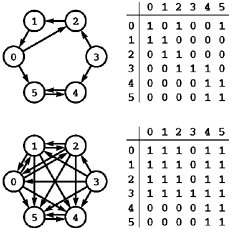
\includegraphics[scale=.7]{informatika/teoreticka_informatika/obrazky/tranzuzaver.png}
    \caption{Tranzitivní uzávěr grafu (zdroj: http://zorro.fme.vutbr.cz/graphs/foil36.html)}
  \end{center}
\end{figure}

\begin{poznamka}
  Platí, že matice dosažitelnosti v grafu $G$ = matice sousednosti tranzitivního
  uzávěru grafu $G$.
\end{poznamka}

\begin{obecne}{Algoritmus}
Z každého vrcholu vypustit DFS (Depth-first search~-- prohledávání do hloubky), do společné matice zaznamenávat dosažené vrcholy (řádek odpovídá vrcholu, sloupce vrcholům, které jsou z něho dosažitelné) -- složitost $O(n(n+m))$.
\end{obecne}

\begin{obecne}{Warshallův algoritmus}
Iterativní konstrukce matice dosažitelnosti, postupně počítá matice $W_k$, kde $w^{[k]}_{i, j} = 1$, pokud mezi vrcholy $i$ a $j$ existuje cesta, jejíž všechny vnitřní vrcholy jsou mezi vrcholy $1\dots k$.

Z matice $W_k$ lze spočítat matici $W^{[k+1]}: W^{[k+1]}_{i,j} = W^{[k]}_{i,j}  || (W^{[k]}_{i,k+1} \&\& W^{[k]}_{k+1,j})$ -- buď vede mezi vrcholy $i, j$ cesta, která nepoužije vrchol $k+1$, nebo taková, která ho použije -- v tom případě ale musí vést cesty mezi vrcholy $i,k+1$ a $k+1,j$, které používají pouze vrcholy $1\dots k$, jejich spojením je cesta mezi vrcholy $i,j$

Matice $W^1$ je matice incidence původního grafu.

Pseudokód (vstup: I -- matice incidence, $[0,1]^{n\times n}$):
\begin{verbatim}
Procedure Warshall(I)
W:= I;
for k:=1 to n
begin
  for i:=1 to n
  begin
    for j:=1 to n
\end{verbatim}
      $w_{i,j} = w_{i,j} || (w_{i,k} \&\& w_{k,j})$
\begin{verbatim}
  end
end 
return W;
\end{verbatim}

Složitost algoritmu je jasně $O(n^3)$ (potřebuje $2n^3$ bitových operací), což může být lepší pro grafy s hodně hranami (počet hran se blíží $n^2$), než složitost $n*DFS$ ( $n*(n + m) ≈ n * (n + n^2) = n^2 + n^3$ )

\end{obecne}

TODO: ještě něco?

\subsection{Algoritmy vyhledávání v textu}
Toto sú len veľmi stručné výťahy z wikipedie. Aktuálne sú tu len preto, aby si človek rýchlo vybavil, o čom tie algoritmy sú :-)

\subsubsection*{Rabin-Karp}
Umožňuje vyhľadávanie viacerých reťazcov v texte naraz - užitočné napr. na hľadanie plagiátov. Základnou myšlienkou je vyhľadávanie v texte pomocou hashov (rolling hashes - idea je \texttt{s[i+1..i+m] = s[i..i+m-1] - s[i] + s[i+m]})...

Algoritmus pre vyhľadávanie jedného reťazca:
\begin{verbatim}
 1 function RabinKarp(string s[1..n], string sub[1..m])
 2     hsub := hash(sub[1..m])
 3     hs := hash(s[1..m])
 4     for i from 1 to n-m+1
 5         if hs = hsub
 6             if s[i..i+m-1] = sub
 7                 return i
 8         hs := hash(s[i+1..i+m])
 9     return not found
\end{verbatim}

Najhoršia zložitosť je $\Omega(mn)$. Pri vyhľadávaní viacerých reťazcov len spočítame hashe všekých hľadaných stringov a pri nájdení niektorého z hashov príslušný reťazec porovnáme s textom... Ostatné algoritmy spotrebujú čas $O(n)$ na nájdenie 1 reťazca a teda $O(nk)$ na vyhľadanie $k$ reťazcov. Naproti tomu tento algoritmus má očakávanú zložitosť $O(n+k)$ - pretože vyhľadávanie v hashovacej tabuľke, či je hash podreťazca textu rovný hashu niektorého z hľadaného reťazcov, trvá $O(1)$.

\subsubsection*{Aho-Corasick}

Dokáže vyhľadávať viacero reťazcov naraz - používa na to trie-like štruktúru (konečný automat), ktorý obsahuje nasledujúce \uv{prvky}:
\begin{penumerate}
	\item konečná množina $Q$ - stavy
	\item konečná abeceda $A$
	\item transition funkcia $g$: $Q \times A \rightarrow Q + \{fail\}$
	\item failure funkcia $h$: $Q \rightarrow Q + \{fail\}$. $h(q)=q'$ práve vtedy keď spomedzi všetkých stavov Q dáva $q'$ najdlhší suffix z $path(q)$.
	\item konečná množina $F$ - koncové stavy
\end{penumerate}

Príklad \uv{hotového} automatu pre slová P=\{ab, ba, babb, bb\}:

\par\begin{center}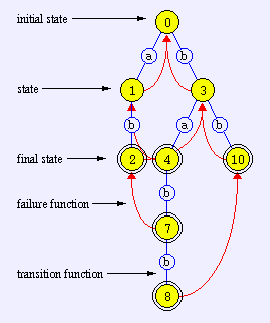
\includegraphics[width=8cm]{informatika/algoritmy_a_ds/obrazky/ahocorasick-automatron.png}\end{center}

Zložitosť vyhľadávania je lineárna vzhľadom k dĺžke textu a počtu nájdených \uv{slov} (pozn.: ten môže byť až kvadradický - slovník a, aa, aaa, aaaa; reťazec aaaa). Trie štruktúru je možné vyrobiť raz a potom používať počas vyhľadávania - uchovávame si najdlší match a používame suffix odkazy (aby sme udržali linearitu výpočtu).

Výstavba stromu se provede prostým zařazováním slov do trie-stromu podle prefixů. Na této struktuře je potom možné v lineárním čase (vzhledem k počtu znaků hledaných slov) předpočítat hodnoty failure funkce: automat vždy pustíme na sufix aktuálně zkoušeného slova, bez prvního znaku. Díky tomu, že průběžně ukládáme hodnoty nalezených slov, pro každé písmeno provede max. 2 kroky (postup vpřed a uložení hodnoty, kam bych spadnul).


\subsubsection*{Knuth-Morris-Pratt}

Obdoba Aho-Corasick, ale hľadá len jedno slovo. Samozrejme nie je potrebná dopredná funkcia (vždy iba nasledujúci znak), používa sa \uv{partial match} tabuľka (failure funkcia).

\begin{verbatim}
algorithm kmp_search:
    input:
        S (the text to be searched)
        W (the word sought)

    m = 0 (the beginning of the current match in S)
    i = 0 (the position of the current character in W)
    an array of integers, T (the table, computed elsewhere)

    while m + i is less than the length of S, do:
        if W[i] = S[m + i],
            i = i + 1
            if i equals the length of W,
                return m
        otherwise,
            m = m + i - T[i],
            if i is greater than 0,
                i = T[i]

    (if we reach here, we have searched all of S unsuccessfully)
    return the length of S
\end{verbatim}

Zložitosť algoritmu je je $O(k)$ (k je dĺžka S) - cyklus je vykonaný najviac $2k$ krát.

Algoritmus na výrobu tabuľky:
\begin{verbatim}
algorithm kmp_table:
    input:
        W (the word to be analyzed)
        T (the table to be filled)

    i = 2 (the current position we are computing in T)
    j = 0 (the zero-based index in W of the next
           character of the current candidate substring)

    (the first few values are fixed but different
          from what the algorithm might suggest)
    let T[0] = -1
    T[1] = 0

    while i is less than the length of W, do:
        (first case: the substring continues)
        if W[i - 1] = W[j],
            T[i] = j + 1
            i = i + 1
            j = j + 1

        (second case: it doesn't, but we can fall back)
        otherwise, if j > 0,
            j = T[j]

        (third case: we have run out of candidates. Note j = 0)
        otherwise,
            T[i] = 0
            i = i + 1
\end{verbatim}


Zložitosť tohoto algoritmu je $O(n)$ (n je dĺžka W) - cyklus skončí najviac po $2n$ iteráciách.

\subsection{Algebraické algoritmy}

\subsubsection*{Diskrétní Fourierova Transformace (DFT)}

Diskrétní Fourierova transformace se používá, chceme-li zachytit hodnotu (přepokládejme, že $2\pi$-periodické) funkce na intervalu $[-\pi,\pi]$ v nějakých $n$ bodech. To je dobré např. pro vzorkování elektrického nebo zvukového signálu a jiné operace. Pro nějakou funkci nám tak stačí znát vektor dimenze $n$ (a $n$ je počet vzorků na $2\pi$).

Je to založeno na Fourierových řadách -- dá se ukázat, že funkce $1$, $\cos kx$ a $\sin kx$ pro $k\geq 1$ tvoří ortogonální bázi prostoru spojitých funkcí na intervalu $[-\pi,\pi]$. Protože potřebujeme znát jenom konečný počet vzorků, stačí nám jen konečný podprostor s konečnou bází. Máme-li rozklad nějaké $2\pi$-periodické funkce do Fourierovy řady $f(x)= c + \sum_{k=1}^\infty a_k \sin k x + \sum_{k=1}^\infty b_k \cos k x$, dá se jednoduše ukázat, že pro hodnoty v bodech $-\pi,-\pi + \frac{\pi}{n}, -\pi + 2\frac{\pi}{n}, \dots, -\pi + (n-1)\frac{\pi}{n}$ stačí sumy do $\frac{n}{2}-1$ pro sinusové řady a $\frac{n}{2}$ pro kosinové -- vyšší koeficienty v takových bodech jsou nulové. Takže $n$ hodnot funkce $f$ na intervalu $[-\pi,\pi]$ lze reprezentovat vektorem $n$ čísel v bázi $1,\cos x,\dots,\cos \frac{n}{2}x,\sin x,\dots,\sin(\frac{n}{2}-1)x$. 

Jednodušeji to lze ukázat v komplexních číslech -- je známo, že 
$$e^{ix} = \cos x+ i\cdot\sin x$$
takže vektor hodnot funkce lze ekvivalentně reprezentovat v bázi $e^{i\cdot 2\pi\frac{k}{n}},\ k\in\{0,\dots,n\}$, neboť všechny vektory původní báze lze zapsat jako lineární kombinace vektorů nové báze. Definujeme hodnotu
$$\omega := e^{i\cdot 2\pi\frac{1}{n}} \textrm{ (a to je vlastně \uv{něco jako} }\sqrt[n]{1}\textrm{)}$$
vidíme, že $\omega^k$ je $n$-periodická funkce, takže nezáleží na hranicích sumace ($-\frac{n}{2}+1,\dots,\frac{n}{2}$ je ekvivalentní $0,\dots,n-1$). 
Potom se posloupnost $n$ komplexních čísel $\alpha_0, \dots, \alpha_{n-1}$ (např. hodnot naší funkce v bodech $-\pi + \frac{2\pi k}{n},\ k\in\{0,\dots,n-1\}$) transformuje na posloupnost $n$ komplexních čísel $A_0, \dots, A_{n-1}$ (do báze $\omega^i,\ i\in\{0,\dots,n-1\}$) použitím vzorečku:
$$A_j = \sum_{k=0}^{n-1} \alpha_k \omega^{kj}  \;\;\;\;\; j = 0, \dots, n-1$$
Tento převod označujeme jako \emph{diskrétní Fourierovu transformaci}.

\emph{Inverzní diskrétní Fourierova transformace} je opačný problém -- z $n$ Fourierových koeficientů $A_k$ chceme zpětně vypočítat hodnoty funkce $\alpha_k$ v bodech $-\pi + \frac{2\pi k}{n},\ k\in\{0,\dots,n-1$. Platí:

$$\alpha_j = \frac{1}{n}\sum_{k=0}^{n-1} A_k \omega^{-kj}  \;\;\;\;\; j = 0, \dots, n-1$$

\medskip
\begin{dukaz}
Definujeme matici $W: W_{p,q}=\omega^{pq}$, potom $A = W\alpha$ (vektorově), takže $a = W^{-1}A$. Definujeme $W': W'_{p,q}=\omega^{-pq}$ a dokážeme, že $W\cdot W'= n\cdot I_n$. Máme
$$(W\cdot W')_{p,q} = \sum_{s=0}^{n-1} W_{p,s}\cdot W'_{s,q} = \sum_{s=0}^{n-1} \omega^{(p-q)\cdot s}$$
a potom pro
\begin{pitemize}
    \item $p = q$ platí $\sum_{s=0}^{n-1}\omega^{(p-q)\cdot s} = \sum_{s=0}^{n-1}\omega^0 = \sum_{s=0}^{n-1} 1 = n$
    \item $p\neq q$ definujeme
    $$Q:= \omega^{p-q}$$
    a dostaneme geometrickou posloupnost $Q^0 + Q^1 +\dots +Q^{n-1}$, pro jejíž součet prvních $n$ členů platí vzorec
    $$ \sum_{s=0}^{n-1} Q^s = Q^0 \frac{Q^{n-1+1} - 1}{Q-1} = 1\frac{1-1}{Q-1}= 0 $$
\end{pitemize}
\end{dukaz}


\begin{algoritmusN}{Fast Fourier transform (FFT)}
Fast Fourier transform je algoritmus pro počítání diskrétní Fourierovy transformace vektorů rozměru $n=2^k$ v čase $\Theta(n\log n)$. Mám-li matici Fourierových koeficientů $W, W_{p,q} = \alpha_q \omega^{pq}$, mohu ji rozdělit na liché a sudé sloupce, u sudých vyjádřit $\omega^q$ a pro spodní polovinu řádek (se sumami jdoucími po dvou) mohu snížit exponent u $\omega$ o $n/2$ (díky periodicitě) a vyjdou stejná čísla:
\begin{align*}
    A_j &= \sum_{k=0}^{n-1} \alpha_k \omega^{kj}\ &j\in\{0,\dots,n-1\}\\
    \\
    A_j &= \sum_{k=0}^{\frac{n}{2}-1} \alpha_{2k}\omega^{2kj} + \omega^j \sum_{k=0}^{\frac{n}{2}-1} \alpha_{2k+1}\omega^{2kj}\ &j\in\{0,\dots,\frac{n}{2}-1\}\\    
    A_{j+\frac{n}{2}} &= \sum_{k=0}^{\frac{n}{2}-1} \alpha_{2k}\omega^{2k(j+\frac{n}{2})} + \omega^{(j+\frac{n}{2})} \sum_{k=0}^{\frac{n}{2}-1} \alpha_{2k+1}\omega^{2k(j+\frac{n}{2})}\ &j\in\{0,\dots,\frac{n}{2}-1\}\\
\end{align*}

\textit{Poznámka: pro rychlé a jednoduché pochopení těch blektů co jsem tu napsal doporučuji Kučerův program Algovision}\\ \texttt{http://kam.mff.cuni.cz/\~{}ludek/AlgovisionPage.html} \\ \textit{DFT je tam názorně a přehledně ukázaná.}
\end{algoritmusN}

TODO: Související obecné \uv{věci} o Fourierově transofrmaci, použití při spektrální analýze (Nyquist-Shannon sampling theorem), datové kompresi (Diskrétní kosinová transformace), násobení polynomů (+násobení velkých integerů).

\subsubsection*{Euklidův algoritmus}

Euklidův algoritmus je postup (algoritmus), kterým lze určit největšího společného dělitele dvou přirozených čísel, tzn. nejvyšší číslo takové, že beze zbytku dělí obě čísla.

Algoritmus (pomocí rekurze):
\begin{verbatim}
function gcd(a, b)
    if b = 0 return a
    else return gcd(b, a mod b)
\end{verbatim}

Algoritmus (pomocí iterace):
\begin{verbatim}
function gcd(a, b)
    while b ≠ 0
        t := b
        b := a mod b
        a := t
    return a
\end{verbatim}

Algoritmus (jednoduchý ale neefektivní):
\begin{verbatim}
function gcd(a, b)
    while b ≠ 0
        if a > b
            a := a - b
        else
            b := b - a
    return a
\end{verbatim}

Doba provádění programu je závislá na počtu průchodů hlavní smyčkou. Ten je maximální tehdy, jsou-li počáteční hodnoty u a v rovné dvěma po sobě jdoucím členům Fibonacciho posloupnosti. Maximální počet provedených opakování je tedy $\log_\phi (3-\phi)v \approx 4{,}785 \log v + 0{,}6273 = O(\log v)$. Průměrný počet kroků pak je o něco nižší, přibližně $\frac{12 \ln 2}{\pi^2}\log v \approx 1{,}9405 \log v = O(\log v)$.

\subsection{Základy kryptografie, RSA, DES}

\subsubsection*{Základy kryptografie}
TODO

\subsubsection*{RSA (Rivest-Shamir-Adleman)}
Asymetrická šifra (různé klíče pro šifrování a dešifrování), použitelná jako šifra s veřejným klíčem.

\textbf{Inicializace:}
\begin{penumerate}
	\item vybrat dvě dostatečně velká prvočísla $p$, $q$
	\item $n:= p\cdot q$
	\item spočítat totient: $\varphi(n) := (p-1)\cdot (q-1)$\\ 
	(Eulerův totient $\varphi(n)$ je počet čísel menších než $n$, která jsou s $n$ nesoudělná)
	\item vybrat $e$ takové, že $1 < e < \varphi(n)$ a $e$ je nesoudělné s $\varphi(n)$\\ -- $e$ bude \emph{veřejný klíč (public key)}
	\item vybrat $d$ tak, aby 
		$$d\cdot e \equiv 1 \mod \varphi(n)$$ 
		takové $d$ lze najít rozšířeným euklidovým algoritmem\\
		-- $d$ bude \emph{dešifrovací klíč (private key)}
\end{penumerate}

\textbf{Šifrování:}
\begin{penumerate}
	\item Alice posílá public key Bobovi (čísla $n$ a $e$), nechává si private key
	\item Bob chce Alici poslat zprávu $m$ (musí být převedena na celé číslo $m < n$)
	\item Bob spočítá :
		$$c = m^e \mod n$$
	\item Bob odešle $c$ Alici
\end{penumerate}

\textbf{Dešifrování:}
\begin{penumerate}
\item Alice přijala $c$
\item Spočítá:
	$$m = c^d \mod n$$
\end{penumerate}

Šifra (to, že to vůbec funguje, tedy, že $m = (m^e)^d$) se opírá o několik netriviálních vět algebry...

\subsubsection*{DES (Data Encryption Standard)}
\begin{pitemize}
\item bloková šifra (vstup plaintext - 64bitů, výstup ciphertext 64bitů)
\item symetrický klíč (stejný pro šifrování i dešifrování) -- strany si ho musí vyměnit po bezpečném kanále
\item klíč -- 64bitů, z nich se používá ale pouze 56bitů (zbytek se zahodí nebo funguje jako kontrola parity)
\item původně implementována hardwarem
\item stejný algoritmus (i hardware) použitý jak pro šifrování, tak pro dešifrování
\end{pitemize}

\begin{figure}[ht]
  \begin{center}
    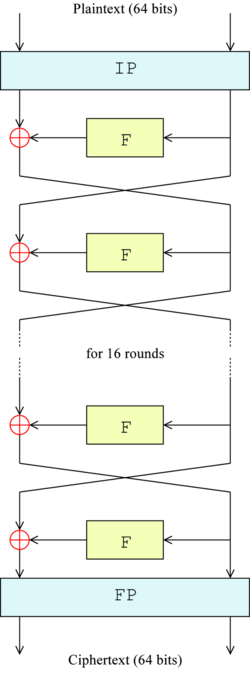
\includegraphics[width=5cm, angle=90]{informatika/siete_a_bezpecnost/obrazky/des-main-network.png}
    \caption{Schéma hlavní sítě algoritmu DES}
  \end{center}
\end{figure}

\begin{obecne}{Šifrování:}
\begin{pitemize}
	\item vstup projde iniciální permutací (IP:64b $\rightarrow$ 64b), na konci probíhá inverzní finální permutace (FP), následuje 16 identických kol šifrování:
	\item blok 64 bitů se rozdělí na dvě půlky po 32bitech, 
	\begin{pitemize}
		\item pravá půlka slouží jako vstup pro funkci F a také je v dalším kole použita jako levá část
		\item levá půlka se xoruje s výstupem funkce F a výsledek je použit v dalším kole jako pravá část
	\end{pitemize}
	\item celý cyklus se provede 16x a v závěru se ještě aplikuje finální permutace
\end{pitemize}
\end{obecne}

\begin{figure}[ht]
  \begin{center}
    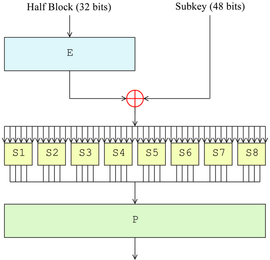
\includegraphics[width=6cm]{informatika/siete_a_bezpecnost/obrazky/des-f-function.png}
    \caption{Funkce \emph{F} v algoritmu DES}
  \end{center}
\end{figure}

\begin{obecne}{Funkce F:}
\begin{pitemize}
	\item ve funkci F probíhá míchání s klíčem. V každém kole vstupuje do funkce F 32bitů z \uv{pravé půlky} a 48bitový subklíč (odvozen z 56bitového klíče, detaily později).
	\item 32bitů z pravé půlky je nejprve expandováno na 48 bitů (fixní expanzní permutací, na obrázku označena E), potom xorováno se subklíčem. 
	\item Výsledek xorování se rozdělí na 8 bloků po 6bitech. Každý blok je pak vstupem jedné z osmi S funkcí. Každá S funkce převádí 6 bitů na 4 bity (nelineární transformací, \uv{zadrátované}).
	\item Výstupy S funkcí se opět spojí do jednoho bloku (8x4 = 32bitů) -- to je výsledek celé funkce F.
\end{pitemize}
\end{obecne}

\begin{obecne}{Dešifrování:} 
Díky prohazování poloviček v jednotlivých kolech lze dešifrování provádět stejnou funkcí (na stejném hardwaru), jako šifrování. Pouze je potřeba používat subklíče v opačném pořadí.
\end{obecne}

\begin{figure}[ht]
  \begin{center}
    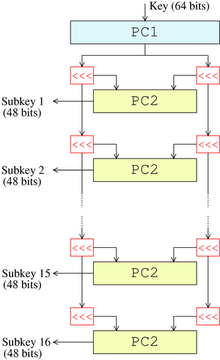
\includegraphics[width=6cm]{informatika/siete_a_bezpecnost/obrazky/des-key-schedule.png}
    \caption{Subklíče v algoritmu DES}
  \end{center}
\end{figure}

\begin{obecne}{Subklíče:}
\begin{pitemize}
	\item protože je klíč původně 64bitový, ale ve skutečnosti se používá pouze 56bitů (ostatní se zahazují, nebo slouží pro kontrolu parity), nejprve je vybráno těchto 56bitů funkcí PC1 (Permuted Choice 1) 
	\item Dále se vždy pro každé kolo 56 bitů rozdělí na dvě půlky po 28bitech. Každá z těchto půlek se bitově posune doleva (o jeden nebo dva bity, to je pevně určeno pro každé kolo). Takto posunuté půlky se vloží jako vstup funkce PC2, která vygeneruje 48bitový subklíč. Obě půlky také slouží jako vstup pro další kolo. 
	\item Algoritmus zaručuje, že každý bit z původního 56bitového klíče je použit asi ve 14-ti ze 16-ti subklíčů. 
	\item Pro dešifrování se klíče musí generovat v opačném pořadí (místo doleva se posouvá doprava).
\end{pitemize}
\end{obecne}



\section{Databáze}
\begin{pozadavky}
\begin{pitemize}
\item Podstata a architektury DB systémů
\item Konceptuální, logická a fyzická úroveň pohledů na data
\item Algoritmy návrhu schémat relací, normální formy, referenční integrita
\item Transakční zpracování, vlastnosti transakcí, uzamykací protokoly, zablokování
\item ER-diagramy, metody návrhů IS
\item SQL
\item Indexy, triggery, uložené procedury, uživatelé, uživatelská práva
\item Vícevrstevné architektury
\item Vazba databází na internetové technologie
\item Organizace dat na vnější paměti, B-stromy a jejich varianty.
\end{pitemize}
\end{pozadavky}
\subsection{Podstata a architektury DB systemů}

Zdroje: Wikipedie, slidy Dr. T. Skopala k Databázovým systémům
\bigskip

\begin{definiceN}{Databáze}
Databáze je logicky uspořádaná (integrovaná) kolekce navzájem souvisejících dat. Je sebevysvětlující, protože data jsou uchovávána společně s popisy, známými jako metadata (také schéma databáze). Data jsou ukládána tak, aby na nich bylo možné provádět strojové dotazy -- získat pro nějaké parametry vyhovující podmnožinu záznamů.

Někdy se slovem \uv{databáze} myslí obecně celý databázový systém.
\end{definiceN}

\begin{definiceN}{Systém řízení báze dat}
Systém řízení báze dat (SŘBD, anglicky database management system, DBMS) je obecný softwarový systém, který řídí sdílený přístup k databázi, a poskytuje mechanismy, pomáhající zajistit bezpečnost a integritu uložených dat. Spravuje databázi a zajišťuje provádění dotazů.
\end{definiceN}

\begin{definiceN}{Databázový systém}
Databázovým systémem rozumíme trojici, sestávající z:
\begin{pitemize}
    \item databáze
    \item systému řízení báze dat
    \item chudáka admina
\end{pitemize}
\end{definiceN}

\begin{obecne}{Smysl databází}
Hlavním smyslem databáze je schraňovat datové záznamy a informace za účelem:
\begin{pitemize}
    \item sdílení dat více uživateli,
    \item zajištění unifikovaného rozhraní a jazyků definice dat a manipulace s daty,
    \item znovuvyužitelnosti dat,
    \item bezespornosti dat a
    \item snížení objemu dat (odstranění redundance).
\end{pitemize}
\end{obecne}

\subsubsection*{Databázové modely}

\begin{definiceN}{schéma, model}
Typicky pro každou databázi existuje strukturální popis druhů dat v ní udržovaných, ten nazýváme \emph{schéma}. Schéma popisuje objekty reprezentované v databázi a vztahy mezi nimi. Je několik možných způsobů organizace schémat (modelování databázové struktury), známých jako \emph{modely}. V modelu jde nejen o způsob strukturování dat, definuje se také sada operací nad daty proveditelná. Relační model například definuje operace jako \uv{select} nebo \uv{join}. I když tyto operace se nemusejí přímo vyskytovat v dotazovacím jazyce, tvoří základ, na kterém je jazyk postaven. Nejdůležitější modely v této sekci popíšeme.
\end{definiceN}

\begin{poznamka}
Většina databázových systémů je založena na jednom konkrétním modelu, ale čím dál častější je podpora více přístupů. Pro každý logický model existuje více fyzických přístupů implementace a většina systémů dovolí uživateli nějakou úroveň jejich kontroly a úprav, protože toto má velký vliv na výkon systému. Příkladem nechť jsou indexy, provozované nad relačním modelem.
\end{poznamka}

\begin{obecne}{\uv{Plochý} model}
Toto sice nevyhovuje úplně definici modelu, přesto se jako triviální případ uvádí. Představuje jedinou dvoudimensionální tabulku, kde data v jednom sloupci jsou považována za popis stejné vlastnosti (takže mají podobné hodnoty) a data v jednom řádku se uvažují jako popis jediného objektu.
\end{obecne}

\begin{obecne}{Relační model}
Relační model je založen na predikátové logice a teorii množin. Většina fyzicky implementovaných databázových systémů ve skutečnosti používá jen aproximaci matematicky definovaného relačního modelu. Jeho základem jsou \emph{relace} (dvoudimensionální tabulky), \emph{atributy} (jejich pojmenované sloupce) a \emph{domény} (množiny hodnot, které se ve sloupcích můžou objevit). Hlavní datovou strukturou je tabulka, kde se nachází informace o nějaké konkrétní  třídě entit. Každá entita té třídy je potom reprezentována řádkem v tabulce -- $n$-ticí atributů.

Všechny relace (tj. tabulky) musí splňovat základní pravidla -- pořadí sloupců nesmí hrát roli, v tabulce se nesmí vyskytovat identické řádky a každý řádek musí obsahovat jen jednu hodnotu pro každý svůj atribut. Relační databáze obsahuje více tabulek, mezi kterými lze popisovat vztahy (všech různých kardinalit, tj. $1:1$, $1:n$ apod.). Vztahy vznikají i implicitně např. uložením stejné hodnoty jednoho atributu do dvou řádků v tabulce. K tabulkám lze přidat informaci o tom, která podmnožina atributů funguje jako \emph{klíč}, tj. unikátně identifikuje každý řádek, některý z klíčů může být označen jako primární. Některé klíče můžou mít nějaký vztah k vnějšímu světu, jiné jsou jen pro vnitřní potřeby schématu databáze (generovaná ID).
\end{obecne}

\begin{obecne}{Hierarchický model}
V hierarchickém modelu jsou data organizována do stromové struktury -- každý uzel má odkaz na nadřízený (k popisu hierarchie) a setříděné pole záznamů na stejné úrovni. Tyto struktury byly používány ve starých mainframeových databázích, nyní je můžeme vidět např ve struktuře XML dokumentů. Dovolují vztahy $1:N$ mezi dvěma druhy dat, což je velice efektivní k popisu různých reálných vztahů (obsahy, řazení odstavců textu, tříděné informace). Nevýhodou je ale nutnost znát celou cestu k záznamu ve struktuře a neschopnost systému reprezentovat redundance v datech (strom nemá cykly).
\end{obecne}

\begin{obecne}{Síťový model}
Síťový model organizuje data pomocí dvou hlavních prvků, \emph{záznamů} a \emph{množin}. Záznamy obsahují pole dat, množiny definují vztahy $1:N$ mezi záznamy (jeden \emph{vlastník}, mnoho \emph{prvků}). Záznam může být vlastníkem i prvkem v několika různých množinách. Jde vlastně o variantu hierarchického modelu, protože síťový model je také založen na konceptu více struktur nižší úrovně závislých na strukturách úrovně vyšší. Už ale umožňuje reprezentovat i redundantní data. Operace nad tímto modelem probíhají \uv{navigačním} stylem: program si uchovává svoji současnou pozici mezi záznamy a postupuje podle závislostí, ve kterých se daný záznam náchází. Záznamy mohou být i vyhledávány podle klíče. 

Fyzicky jsou většinou množiny -- vztahy -- reprezentovány přímo ukazateli na umístění dat na disku, což zajišťuje vysoký výkon při vyhledávání, ale zvyšuje náklady na reorganizace. Smysl síťové navigace mezi objekty se používá i v objektových modelech.
\end{obecne}

\begin{obecne}{Objektový model}
Objektový model je aplikací přístupů známých z objektově-orientovaného programování. Je založen na sbližování programové aplikace a databáze, hlavně ve smyslu použití datových typů (objektů) definovaných na jednom místě; ty zpřístupňuje k použití v nějakém běžném programovacím jazyce. Odstraní se tak nutnost zbytečných konverzí dat. Přináší do databází také věci jako zapouzdření nebo polymorfismus. Problémem objektových modelů je neexistence standardů (nebo spíš produktů, které by je implementovaly).

Kombinací objektového a relačního přístupu vznikají \emph{objektově-relační} databáze -- relační databáze, dovolující uživateli definovat vlastní datové typy a operace na nich. Obsahují pak hybrid mezi procedurálním a dotazovacím programovacím jazykem.

\end{obecne}


\subsubsection*{Architektury databázových systémů}

Zdroj: Wiki ČVUT (státnice na FELu ;-))
\bigskip

Architektury databázových systémů se obecně dělí na 
\begin{pitemize}
    \item \emph{centralizované} (kde se databáze předpokládá fyzicky na jednom počítači) a
    \item \emph{distribuované},
\end{pitemize}
případně na
\begin{pitemize}
    \item \emph{jednouživatelské} a
    \item \emph{víceuživatelské}.
\end{pitemize}

\begin{obecne}{Distribuované databázové systémy}
\emph{Distribuovaný systém řízení báze dat} je vlastně speciálním případem obecného distribuovaného výpočetního systému. Jeho implementace zahrnuje fyzické rozložení dat (včetně možných replikací databáze) na více počítačů -- \emph{uzlů}, přičemž jejich popis je integrován v globálním databázovém schématu. Data v uzlech mohou být zpracovávána lokálními SŘBD, komunikace je organizována v síťovém provozu pomocí speciálního softwaru, který umí zacházet s distribuovanými daty. Fyzicky se řeší rozložení do uzlů, svázaných komunikačními kanály, a jeho transparence (neviditelnost -- navenek se má tvářit jako jednolitý systém). Každý uzel v síti je sám o sobě databázový systém a z každého uzlu lze zpřístupnit data kdekoliv v síti.

Dále se dělí na dva typy:
\begin{pitemize}
    \item Federativní databáze -- neexistuje globální schéma ani centrální řídící autorita, řízení je také distribuované.
    \item Heterogenní databázové systémy -- jednotlivé autonomní SŘBD existují (vznikly nezávisle na sobě) a jsou integrovány, aby spolu mohly komunikovat.
\end{pitemize}

Výhodou oproti centralizovaným systémům je vyšší efektivita (data mohou být uložena blízko místa nejčastějšího používání), zvýšená dostupnost, výkonnost a rozšiřitelnost; nevýhodou zůstává problém složitosti implementace, distribuce řízení a nižší bezpečnost takových řešení.
\end{obecne}

\begin{obecne}{Víceuživatelské databázové systémy}
\emph{Víceuživatelské} jsou takové systémy, které umožňují vícenásobný uživatelský přístup k datům ve stejném okamžiku. V důsledku možného současného přístupu více uživatelů je nutné systém zabezpečit tak, aby i nadále zajišťoval integritu a konzistenci uložených dat. Existují obecně dva možné přístupy:
\begin{pitemize}
    \item Uzamykání -- Dříve často používaná metoda založená na uzamykání aktualizovaných záznamů, v případě masivního využití aktualizačních příkazů u ní ale může docházet k značným prodlevám. 
    \item Multiversion Concurency Control -- Modernější vynález. Jeho princip spočívá v tom, že při požadavku o aktualizaci záznamu v tabulce je vytvořena kopie záznamu, která není pro ostatní uživatele až do provedeného commitu viditelná.
\end{pitemize}
\end{obecne}

\subsection{Konceptualní, logická a fyzická úroveň pohledu na data}

TODO: sjednotit terminologii, snad to popisuje to co tu má být, ale zdroje jsou pochybné (Wikipedie tady neodvádí zrovna ideální práci a ČVUT Wiki se moc nerozepisuje).

\begin{definiceN}{Datové modelování}
\emph{Datové modelování} je proces vytvoření konkrétního datového modelu (schématu) databáze pomocí aplikace nějakého abstraktního databázového modelu. Datové modelování zahrnuje kromě definice struktury a organizace dat ještě další implictiní nebo explicitní omezení na data do struktury ukládaná. 
\end{definiceN}

\begin{obecne}{Vrstvy modelování}
Druhy datových modelů mohou být tří typů, podle tří různých pohledů na databáze (tři \uv{vrstvy}, které se navzájem doplňují):
\begin{pitemize}
    \item konceptuální schéma (datový model) -- nejabstraktnější, popisuje význam organizace databáze -- třídy entit a jejich vztahy.
    \item logické schéma -- popisuje význam konceptuálního schématu z hlediska databázové implementace -- popisy tabulek, programových tříd nebo XML tagů (podle zvoleného databázového modelu)
    \item fyzické schéma -- nejkonkrétnější, popisuje fyzické uložení dat a stroje na kterých systém poběží.
\end{pitemize}
Na tomto rozdělení je důležitá nezávislost jednotlivých vrstev -- takže se implementace jedné z nich může změnit, aniž by bylo nutné výrazně upravovat ostatní (samozřejmě musí zůstat konzistetní vzhledem k ostatním vrstvám). Během implementace nějaké databázové aplikace se začíná vytvořením konceptuálního schématu, pokračuje jeho upřesnění logickým schématem a naknec jeho fyzickou implementací podle fyzického schématu (modelu).
\end{obecne}

\begin{poznamka}
V tomto pohledu (který je podle standardu ANSI z r. 1975) jsou databázové modely, popsané v předchozí sekci, příklady abstraktních logických datových modelů. Někde je však tato úroveň označována jako \uv{fyzická} a \uv{jiná logická} se vtěsní ještě mezi ni a konceptuální.
\end{poznamka}


\begin{obecne}{Konceptuální schéma}
\emph{Konceptuální schéma} (datový model) popisuje podstatné objekty (\emph{třídy entit}, \uv{koncepty}), jejich charakteristiky (\emph{atributy}) a vztahy mezi nimi (asociace mezi dvojicemi tříd entit). Nepopisuje přímo implementaci v databázi, jen význam nějakého celku, který bude databází představován. Jde o modelování \uv{datové reality}, z pohledu uživatele (analytika, konstruktéra databáze).

\medskip
\begin{priklady}
Pár příkladů vztahů mezi třídami entit (z Wikipedie):
\begin{pitemize}
    \item Each PERSON may be the vendor in one or more ORDERS.
    \item Each ORDER must be from one and only one PERSON.
    \item PERSON is a sub-type of PARTY. (Meaning that every instance of PERSON is also an instance of PARTY.)
\end{pitemize}
\end{priklady}
De-facto standardem pro konceptuální datové modelování jsou \emph{ER-diagramy} (entity-relationship diagramy). Hodí se hlavně pro \uv{plochá} formátovaná data (takže třeba pro objektové nebo relační databáze, ale ne pro XML apod.). Používají dva typy \uv{objektů} -- \emph{entity} (třídy entit) a \emph{vztahy}. Jde o obdobu UML z objektového programování. Příklad ER-diagramu se vztahem dvou entit je na následujícím obrázku (popisuje i další vlastnosti -- atributy entit a kardinality vztahů):
\begin{center}
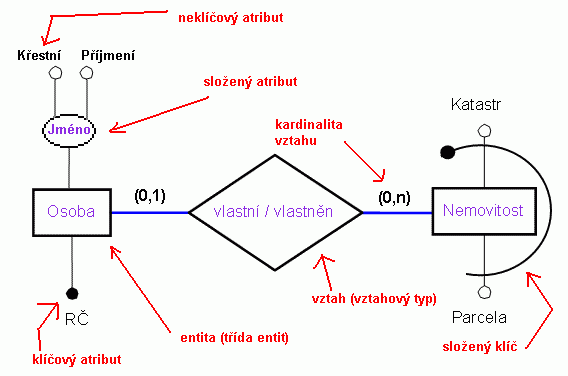
\includegraphics[width=14cm]{informatika/databazy/obrazky/er-schema.png}

(Obrázek je upravený, rozšířený a popsaný příklad ze slidů Dr. T. Skopala k Databázovým systémům)
\end{center}
\end{obecne}

\begin{obecne}{Logické schéma}
\emph{Logické schéma} je datový model organizace nějakého specifického celku pomocí jednoho z databázových modelů -- podle databázových modelů popsaných v předchozí sekci, tj. např. pomocí relačních tabulek, objektových tříd nebo XML. Svojí úrovní abstrakce se nachází mezi konceptuálním a fyzickým schématem.

TODO: to zřejmě nebyl dobrý nápad nacpat datové modely do architektur DB -- vhodnější by to bylo přesunout, je to ale nutné trochu učesat aby seděla terminologie.
\end{obecne}

\begin{obecne}{Fyzické schéma}
\emph{Fyzické datové modely} jsou modely, ktere používají databazové stroje směrem k nižším vrstvám (operačního) systému. V zásadě jde o různé způsoby fyzického uložení dat (tedy schémata organizace souborů) -- sekvenční soubory, B-stromy apod.
\end{obecne}


\subsection{Algoritmy návrhu schémat relací}


\subsubsection*{Normální formy}

\begin{obecne}{Normalizace, anomálie}
Normalizace databází je technika návrhu relačních databázových tabulek, pri které se minimalizují duplicity informací - a zamezuje se tak nekonzistentnosti dat. Stupně normalizace se \uv{popisují} pomocí \emph{normálních forem} - čím vyšší forma, tým vyšší striktnost...

Problémy řešené normalizací:
\begin{pitemize}
	\item \emph{update anomaly} -- př.: tabulka (člověk, adresa, skill); kdyby se nevykonal update správně, může tabulka zůstat v nekonzistentním stavu (např. by se mohly změnit jen některé adresy jednoho člověka)
	\item \emph{insertion anomaly} -- za jistých okolností by se některá fakta nedala zaznamenat, např. v tabulce (fakulta, datum založení, kurz) můžeme zaznamenat jen data pro fakulty, které mají kurzy...
	\item \emph{deletion anomaly} -- za jistých okolností by se mohlo stát, že vymazání některých faktů by způsobilo vymazání dat reprezentujících jiná fakta. V předchozí tabulce bude fakulta vymazána úplně, když se vzdá všech kurzů.
\end{pitemize}

Ideálně by relační databáze měla být navržena tak, aby vylučovala možnost takových anomalií. Normalizace obvykle zahrňuje dekomponování nenormalizované tabulky na dvě nebo více tabulek takových, že po jejich spojení (join) dostaneme všechny původní informace.

Abychom mohli definovat normální formy, potřebujeme znát funkční závislosti jednotlivých atributů entit relační databáze a vědět, které atributy jsou klíčové a které ne.
\end{obecne}

\begin{definiceN}{Funkční závislosti}

\medskip\noindent
Řekneme, že atribut \emph{B} je \textbf{funkčně závislý} na atributu \emph{A}
(značíme $A\rightarrow B$), jestliže pro každou hodnotu atributu \emph{A}
existuje právě jedna hodnota atributu \emph{B}. Rozšířené funkční závislosti se definují pro množinu atributů (pro každou $n$-tici atributů z nějaké množiny existuje právě jedna hodnota závislého(závislých) atributu(atributů)).

Funkční závislosti splňují tzv. \emph{Armstrongova pravidla}, což zahrnuje pro množiny atributů $X,Y,Z$:
\begin{penumerate}
    \item triviální závislost: $X\supseteq Y\ \Rightarrow\ X\to Y$
    \item transitivitu: $X\to Y \wedge Y\to Z\ \Rightarrow\ X\to Z$
    \item kompozici: $X\to Y \wedge X\to Z\ \Rightarrow X\to YZ$
    \item dekompozici: $X\to YZ \ \Rightarrow \ X\to Y \wedge X\to Z$
\end{penumerate}
\end{definiceN}

\begin{definiceN}{Klíč}
\textbf{Nadklíčem}, někdy též \textbf{superklíčem}, schématu $A$ rozumíme každou
podmnožinu množiny $A$, na níž $A$ funkčně závisí. Jinak řečeno nadklíč je množina
atributů, která jednoznačně určuje řádek tabulky.

\textbf{Klíč}, nebo také \textbf{potenciální klíč}(candidate key), schématu $A$
je takový nadklíč schématu $A$, jehož žádná vlastní podmnožina není nadklíčem
$A$. Čili minimální nadklíč.

Každý atribut, který je obsažen alespoň v jednom potenciálním klíči se nazývá
\textbf{klíčový}, ostatní atributy jsou \textbf{neklíčové}.
\end{definiceN}

\begin{definiceN}{Normální formy}
\begin{pitemize}
	\item \emph{První normální forma} \\ -- Tabulka je v první normální formě, jestliže lze do každého pole dosadit pouze jednoduchý datový typ (jsou dále nedělitelné). To zahrnuje i neexistenci více sloupců tabulky se stejným druhem obsahu:
$$
\left.\begin{aligned}
\textrm{(manager, podřízený1, podřízený2, podřízený3)} \\ 
\textrm{(manager, podřízení-vice\_hodnot\_v\_jednom\_sloupci)} \\
\end{aligned}\right\} \rightarrow \textrm{(manager, podřízený)}
$$
	\item \emph{Druhá normální forma} \\ 
-- Existuje klíč a všechna neklíčová pole jsou funkcí celého klíče (a tedy ne jen jeho částí). 
$$\textrm{(custID, name, address, city, state, zip)} \rightarrow
\begin{aligned}&\textrm{(custID, name, address, zip)}\\
&+ \textrm{(zip, city, state)}
\end{aligned}$$
	\item \emph{Třetí normální forma} \\ -- Tabulka je ve třetí normální formě, jestliže každý neklíčový atribut není transitivně závislý na žádném klíči schématu (resp. každý neklíčový atribut je přímo závislý na klíči schématu) neboli je-li ve druhé normální formě a zároveň neexistuje jediná závislost neklíčových sloupců tabulky. 
$$\textrm{(deptID, deptName, managerID, hireDate)} \rightarrow \textrm{(deptID, deptName, managerID)}$$
Atribut \uv{hireDate} je sice funkčně závislý na klíči deptID, ale jen proto, že hireDate závisí na managerID, které závisí na deptID.
	\item \emph{Boyce-Coddova normální forma}\\ -- Pro každou netriviální závislost $X \rightarrow Y$ platí, že $X$ obsahuje klíč schématu $R$ ($X$ je nadklíč).
\end{pitemize}
\end{definiceN}

\subsubsection*{Algoritmy návrhu schémat relací}

Schémata relací by měla být navrhována tak, aby odpovídala předem připravenému konceptuálnímu modelu (např. pomocí ER diagramů) a zároveň pokud možno splňovala co nejpřísnější požadavky na normální formy. Pro modelování relační databáze existují dva přístupy:
\begin{penumerate}
    \item Získání množiny relačních schémat (ručně nebo převodem z např. ER diagramu) a provádění normalizace pro každou tabulku zvlášť
    \item Návrh tzv. univerzálního schématu databáze -- jedna velká tabulka pro celou databázi (vč. platných funkčních závislostí) a normalizace prováděná globálně
\end{penumerate}
První možnost je relativně intuitivní (s ER diagramy) a jednoduchá, ale hrozí riziko přílišného rozdrobení databáze na velký počet malých tabulek (a nadbytečný i vzhledem k požadované normální formě). V druhém způsobu jsou entity jednotlivých relací \uv{vypozorovány} jako efekt funkčních závislostí, což není příliš průhledné a jednoduše proveditelné, ale minimalizuje to šanci na rozdrobení databáze. Oba přístupy lze také zkombinovat -- převést ER model databáze do schémat a některá (nebo až všechna) potom před normalizací sloučit.

\begin{obecne}{Normalizace}
Jediným způsobem, jak u nějakého obecného relačního schématu dosáhnout normální formy (obecně se požaduje většinou 3NF nebo BCNF), je rozdělení na několik podschémat. Dá se to provést ručně nebo algoritmicky a existuje více přístupů podle požadavku na normální formu, \emph{bezztrátovost} (dekompozice relace $R( A, F )$ do $R_1(A_1,F_1)$ a $R_2(A_2,F_2)$ je bezeztrátová, když $A1 \cap A2\to A1$ nebo $A1 \cap A2 \to A2$, tedy opětovným spojením do původní relace nevzniknou další řádky) nebo \emph{pokrytí závislostí} (dekompozice $R(A,F)$ do $R_1(A_1,F_1)$ zachovává pokrytí závislostí, když $F^{+}=F^{+}_1\cup F^{+}_2$ -- nesmí se ztratit závislost ani v rámci dílčího schématu, ani jdoucí napříč schématy).
\end{obecne}

\begin{algoritmusN}{Dekompozice}
Dekompozice je algoritmus, který relační schéma převede do Boyce-Coddovy normální formy. Zaručuje zachování bezeztrátovosti, ale už ne pokrytí závislostí (bez ohledu na algoritmus toto u BCNF někdy není možné). Jeho běh vypadá následovně:
\begin{penumerate}
    \item Vyber nějaké schéma, které není v BCNF.
    \item Vezmi pro něj neklíčovou závislost $X\to Y$ (tak že $X$ není klíč) a dekomponuj podle ní -- vyhoď ze schématu $Y$ a dej $XY$ do zvláštní tabulky.
    \item Opakuj od kroku 1, dokud existuje schéma, které není v BCNF.
\end{penumerate}
\end{algoritmusN}

\begin{algoritmusN}{Syntéza}
Algoritmus syntézy obecně dosahuje třetí normální formy a zachovává pokrytí závislostí (ale ne bezeztrátovost). Pro relační schéma $R$ s množinou funkčních závislostí $F$ vypadá následovně:
\begin{penumerate}
    \item Udělej minimální pokrytí $F$ (vzhledem k tranzitivitě), nazvi ho $G$.
    \item Sluč funkční závislosti z $G$ se stejnou levou stranou a z každé vytvoř jedno schéma. 
    \item Zahoď schémata, která jsou podmnožiny jiných.
\end{penumerate}
Nakonec je možné sloučit schémata s funkčně ekviv. klíči ($K1 \leftrightarrow K2$), ale může to porušit normální formu, které bylo dosaženo! Pro zachování bezeztrátovosti lze do přidat nějaké schéma, obsahující univerzální klíč celého původního (neděleného) schématu.
\end{algoritmusN}

\begin{poznamka}
Pro nalezení minimálního pokrytí atributů se používá pomocný algoritmus, který se chová takto:
\begin{penumerate} 
    \item Dekomponuj všechny funkční závislosti na elementární (na pravé straně je jen jeden sloupec)
    \item Odstraň z nich redundantní atributy (takové z levé strany, které funkčně závisí na jiných z levé strany)
    \item Odstraň redundantní funkční závislosti (tj. takové, které jsou tranzitivním důsledkem jiných -- pravá strana funkčně závisí na levé, i když z množiny funkčních závislostí onu redundantní odstraním)
\end{penumerate}
Pro druhý i třetí krok je potřeba získat \emph{atributový uzávěr} (množina všech atributů i tranzitivně závislých na levé straně) -- to se opakovaně zkouší, jestli díky funkčním závislostem nedostanu z atributů původní množiny nějaké další atributy (dokud nacházím další, přidávám je do množiny a opakuji).
\end{poznamka}

\subsubsection*{Referenční integrita}

\begin{pitemize}
	\item pomáhá udržovat vztahy v relačně propojených databázových tabulkách, zabraňuje vzniku nekonzistentních dat
	\item kontrola přípustných hodnot
	\item kontrola existence položky s daným klíčem v druhé tabulce (podle cizího klíče) 
\end{pitemize}

Chování při porušení integrity:
\begin{pitemize}
	\item ON UPDATE, ON DELETE - podmínka spuštění akce
	\item ON \dots RESTRICT - defaultní řešení (hlášení chyby)
	\item CASCADE - kaskádová aktualizace/smazání (smaže příslušné řádky v odkazované tabulke)
	\item SET NULL - nastavení odkazovaných řádků závislé tabulky na NULL
	\item SET DEFAULT - nastavení pevně určené hodnoty
	\item NO ACTION 
\end{pitemize}

\subsection{Transakční zpracování, vlastnosti transakcí, uzamykací protokoly, zablokování}

\begin{definiceN}{Transakce}
\emph{Transakce} je jistá posloupnost nebo specifikace posloupnosti akcí práce s databází, jako
jsou čtení, zápis nebo výpočet, se kterou se zachází jako s jedním celkem.
\end{definiceN}

Hlavním smyslem používání transakcí, tj. \emph{transakčního zpracování}, je
udržení databáze v konzistentním stavu. Jestliže na sobě některé operace závisí,
sdružíme je do jedné transakce a tím zabezpečíme, že budou vykonány buď
všechny, nebo žádná. Databáze tak před i po vykonání transakce bude v
konzistentním stavu. Aby se uživateli transakce jevila jako jedna atomická
operace, je nutné zavést příkazy COMMIT a ROLLBACK. První z nich signalizuje
databázi úspěšnost provedení transakce, tj. veškeré změny v databázi se stanou
trvalými a jsou zviditelněny pro ostatní transakce, druhý příkaz signalizuje
opak, tj. databáze musí být uvedena do původního stavu.

Tyto příkazy většinou není nutné volat explicitně, např. příkaz COMMIT je vyvolán po
normálním ukončení programu realizujícího transakci. Příkaz ROLLBACK pro svou
funkci vyžaduje použití tzv. \emph{žurnálu} (logu) na nějakém stabilním
paměťovém médiu. Žurnál obsahuje historii všech změn databáze v jisté časové
periodě.

Jednoduchá transakce vypadá většinou takto:
\begin{penumerate}
  \item Začátek transakce,
  \item provedení několika dotazů -- čtení a zápisů (žádné změny v databázi nejsou zatím vidět pro
  okolní svět),
  \item Potvrzení (příkaz COMMIT) transakce (pokud se transakce povedla, změny
  v databázi se stanou viditelné).
\end{penumerate}
Pokud nějaký z provedených dotazů selže, systém by měl celou transakci zrušit a
vrátit databázi do stavu v jakém byla před zahájením transakce (operace ROLLBACK).

Transakční zpracování je také ochrana databáze před hardwarovými nebo
softwarovými chybami, které mohou zanechat databázi po částečném zpracování
transakce v nekonzistentním stavu. Pokud počítač selže uprostřed provádění
některé transakce, transakční zpracování zaručí, že všechny operace z
nepotvrzených (\uv{uncommitted}) transakcí budou zrušeny. 

\subsubsection*{Vlastnosti transakcí}

Podívejme se nyní na vlastnosti požadované po transakcích. Obvykle se používá
zkratka prvních písmen anglických názvů vlastností \textbf{ACID}~-- atomicity,
consistency, isolation (independence), durability. 
\begin{description}
  \item[atomicita] -- transakce se tváří jako jeden celek, musí buď proběhnout
  celá, nebo vůbec ne.
  \item[konzistence] -- transakce transformuje databázi z jednoho konzistentního
  stavu do jiného konzistentního stavu.
  \item[nezávislost] -- transakce jsou nezávislé, tj. dílčí efekty transakce
  nejsou viditelné jiným transakcím.
  \item[trvanlivost] -- efekty úspěšně ukončené (potvrzené,\uv{commited})
  transakce jsou nevratně uloženy do databáze a nemohou být zrušeny.
\end{description}

Transakce mohou být v uživatelských programech prováděny paralelně (spíše
zdánlivě paralelně, stejně jako je paralelismus multitaskingu na jednoprocesorových
strojích jen zdánlivý, zajistí to ale možnost paralelizace \uv{nedatabázových} 
akcí a pomalé transakce nebrzdí rychlé). Je
zřejmé, že posloupnost transakcí může být zpracována paralelně různým způsobem.
Každá transakce se skládá z několika akcí. Stanovené pořadí provádění akcí
více transakcí v čase nazveme \textbf{rozvrhem}.

Rozvrh, který splňuje následující podmínky, budeme nazývat \textbf{legální}:
\begin{pitemize}
  \item Objekt je nutné mít uzamknutý, pokud k němu chce transakce přistupovat.
  \item Transakce se nebude pokoušet uzamknout objekt již uzamknutý jinou
  transakcí (nebo musí počkat, než bude objekt odemknut).
\end{pitemize}

Důležitými pojmy pro paralelní zpracování jsou sériovost či uspořádatelnost.
\textbf{Sériové rozvrhy} zachovávají operace každé transakce pohromadě (a 
provádí se jen jedna transakce najednou). Pro $n$
transakcí tedy existuje $n!$ různých sériových rozvrhů. Pro získání korektního
výsledku však můžeme použít i rozvrhu, kde jsou operace různých transakcí
navzájem prokládány.
Přirozeným požadavkem na korektnost je, aby efekt paralelního zpracování
transakcí byl týž, jako kdyby transakce byly provedeny v nějakém sériovém rozvrhu.
Předpokládáme-li totiž, že každá transakce je korektní program, měl by vést
výsledek sériového zpracování ke konzistentnímu stavu. O systému zpracování
transakcí, který zaručuje dosažení konzistentního stavu nebo stejného stavu
jako sériové rozvrhy, se říká, že zaručuje \textbf{uspořádatelnost}.

Mohou se vyskytnout problémy, které uspořádatelnosti zamezují. Ty nazýváme \emph{konflikty}. Plynou z pořadí dvojic akcí různých transakcí na stejném objektu. Existují tři typy konfliktních situací:
\begin{penumerate}
    \item WRITE-WRITE -- přepsání nepotvrzených dat
    \item READ-WRITE -- neopakovatelné čtení
    \item WRITE-READ -- čtení nepotvrzených (\uv{uncommitted}) dat
\end{penumerate}

Řekneme, že rozvrh je \emph{konfliktově uspořádatelný}, je-li konfliktově ekvivalentní nějakému sériovému rozvrhu (tedy jsou v něm stejné, tj. žádné konflikty). Test na konfliktovou uspořádatelnost se dá provést jako test acykličnosti grafu, ve kterém konfliktní situace představují hrany a transakce vrcholy. Konfliktová uspořádatelnost je slabší podmínka než uspořádatelnost -- nezohledňuje ROLLBACK (\emph{zotavitelnost} -- zachování konzistence, i když kterákoliv transakce selže) a dynamickou povahu databáze (vkládání a mazání objektů). Zotavitelnosti se dá dosáhnout tak, že každá transakce $T$ je potvrzena až poté, co jsou potvrzeny všechny ostatní transakce, které změnily data čtená v $T$. Pokud v zotavitelném rozvrhu dochází ke čtení změn pouze potvrzených transakcí, nemůže dojít ani k jejich \emph{kaskádovému rušení}.

Při zpracování (i uspořádatelného) rozvrhu může dojít k situaci \emph{uváznutí} -- \emph{deadlocku}. To nastane tehdy, pokud jedna transakce $T_1$ čeká na zámek na objekt, který má přidělený $T_2$ a naopak. Situaci lze zobecnit i na více transakcí. Uváznutí lze buď přímo zamezit charakterem rozvrhu, nebo detekovat (hledáním cyklu v grafu čekajících transakcí, tzv. \uv{waits-for} grafu) a jednu z transakcí \uv{zabít} a spustit znova.

\medskip
K zajištění uspořádatelnosti a zotavitelnosti a zabezpečení proti kaskádovým rollbackům a deadlocku se používají různá schémata (požadavky na rozvrhy). Jedním z nich jsou uzamykací protokoly.

\subsubsection*{Uzamykací protokoly}

Vytváření rozvrhů a testování jejich uspořádatelnosti není pro praxi zřejmě ten
nejvhodnější způsob. Pokud ale budeme transakce konstruovat podle určitých
pravidel, tak za určitých předpokladů bude každý jejich rozvrh uspořádatelný.
Soustavě takových pravidel se říká \textbf{protokol}.

Nejznámější protokoly jsou založeny na dynamickém zamykání a odemykání objektů v
databázi. Zamykání (operace LOCK) je akce, kterou vyvolá transakce na objektu,
aby ho chránila před přístupem ostatních transakcí.

\begin{definiceN}{Dobře formovaná transakce}
Transakci nazveme \textbf{dobře formovanou} pokud podporuje přirozené požadavky
na transakce:
\begin{penumerate}
  \item transakce zamyká objekt, chce-li k němu přistupovat,
  \item transakce nezamyká objekt, který již je touto transakcí uzamčený,
  \item transakce neodmyká objekt, který není touto transakcí zamčený,
  \item po ukončení transakce jsou všechny objekty uzamčené touto transakcí
  odemčeny.
\end{penumerate}
\end{definiceN}

\paragraph{Dvoufázový protokol (2PL)} -- Dvoufázová transakce v první fázi
zamyká vše co je potřeba a od prvního odemknutí (druhá fáze) již jen odemyká co
měla zamčeno (již žádná operace LOCK). Tedy transakce musí mít všechny objekty
uzamčeny předtím, než nějaký objekt odemkne. Dá se dokázat, že pokud jsou
všechny transakce v dané množině transakcí dobře formované a dvoufázové, pak
každý jejich legální rozvrh je uspořádatelný.

Dvoufázový protokol zajišťuje uspořádatelnost, ale ne zotavitelnost ani
bezpečnost proti kaskádovému rušení transakcí nebo uváznutí.

\paragraph{Striktní dvoufázový protokol (S2PL)} -- Problémy 2PL jsou nezotavitelnost
a kaskádové rušení transakcí. Tyto nedostatky lze odstranit pomocí striktních
dvoufázových protokolů, které uvolňují zámky až po skončení transakce (COMMIT).
Zřejmá nevýhoda je omezení paralelismu. 2PL navíc stále nevylučuje možnost deadlocku.

\paragraph{Konzervativní dvoufázový protokol (C2PL)} -- Rozdíl oproti 2PL je
ten, že transakce žádá o všechny své zámky, ještě než se začne
vykonávat. To sice vede občas k zbytečnému zamykání (nevíme co přesně budeme
potřebovat, tak radši zamkneme víc), ale stačí to již k prevenci uváznutí
(deadlocku).

\subsubsection*{\uv{Vylepšení} zamykacích protokolů}

\paragraph{Sdílené a výlučné zámky} -- Nevýhodou 2PL je, že objekt může mít
uzamčený pouze jedna transakce. Abychom uzamykání provedli precizněji, je dobré
vzít na vědomí rozdíl mezi operacemi READ a WRITE. \emph{Výlučný zámek}
(W\_LOCK) může být aplikován na objekty jak pro operaci READ tak pro WRITE,
\emph{sdílený zámek} (R\_LOCK) uzamyká objekt, který chceme pouze číst. Jeden
objekt potom může být uzamčen sdíleným zámkem více transakcí a zvyšuje se tak
možnost paralelního zpracování. Budeme-li s těmito zámky zacházet stejně jako u
2PL, opět máme zaručenou uspořádatelnost rozvrhu, ovšem nikoliv absenci uváznutí.


\paragraph{Strukturované uzamykání (multiple granularity)} -- Objekty jsou v
tomto případě chápány hierarchicky dle relace \emph{obsahuje}. Například
databáze obsahuje soubory, které obsahují stránky a ty zase obsahují jednotlivé
záznamy. Na tuto hierarchii se můžeme dívat jako na strom, ve kterém každý
vrchol obsahuje své potomky. Když transakce zamyká objekt (vrchol) zamyká také
všechny jeho potomky. Protokol se tak snaží minimalizovat počet zámků, tím
snížit režii a zvýšit možnosti paralelního zpracování.


\subsubsection*{Alternativní protokoly}

\paragraph{Časová razítka} -- Další z protokolů zaručující uspořádatelnost je
využití časových razítek. Na začátku dostane transakce $T$ \emph{časové
razítko}~-- $TS(T)$ (časová razítka jsou unikátní a v čase rostou), abychom věděli
pořadí, ve kterém by měli být transakce vykonány. Každý objekt v databázi má
\emph{čtecí razítko}~-- $RTS(O)$ (read timestamp), které je aktualizováno, když je
objekt čten, a \emph{zapisovací razítko}~-- $WTS(O)$ (write timestamp), které je
aktualizováno, když nějaká transakce objekt mění.

Pokud chce transakce $T$ číst objekt $O$ mohou nastat dva případy:
\begin{pitemize}

  \item $TS(T) < WTS(O)$, tzn. někdo změnil objekt $O$ potom co byla spuštěna
  transakce $T$. V tomto případě musí být transakce zrušena a spouštěna znovu (a
  tedy s jiným časovým razítkem).

  \item $TS(T) > WTS(O)$, tzn. je bezpečné objekt číst. V tomto případě $T$
  přečte $O$ a $RTS(O)$ je nastaveno na $\max\{TS(T),\ RTS(O)\}$.

\end{pitemize}

Pokud chce transakce $T$ zapisovat do objektu $O$ rozlišujeme případy tři:
\begin{pitemize}

  \item $TS(T) < RTS(O)$, tzn. někdo četl $O$ poté co byla spuštěna $T$ a
  předpokládáme, že si pořídil lokální kopii. Nemůžeme tedy $O$ změnit, protože
  by lokální kopie přestala být platná a tedy je nutné $T$ zrušit a spustit
  znova.

  \item $TS(T) < WTS(O)$, tzn. někdo změnil $O$ po startu $T$. V tomto případě
  přeskočíme write operaci a pokračujeme dále normálně. $T$ nemusí být
  restartována.

  \item V ostatních případech $T$ změní $O$ a $WTS(O)$ je nastaveno na $TS(T)$.
\end{pitemize}

\paragraph{Optimistické protokoly} -- V situaci kdy se většina transakcí
neovlivňuje, je režie výše uvedených protokolů zbytečně velká a můžeme použít
takzvaný optimistický protokol. V protokolu můžeme rozlišit tři fáze.
\begin{penumerate}

  \item \textbf{Fáze čtení:} Čtou se objekty z databáze do lokální paměti a jsou
  na nich prováděny potřebné změny.

  \item \textbf{Fáze kontroly:} Po dokončení všech změn v lokální paměti je
  vyvolán pokus o zapsání výsledků do databáze. Algoritmus zkontroluje, zda
  nehrozí potenciální kolize s již potvrzenými transakcemi, nebo s některými
  právě probíhajícími. Pokud konflikt existuje, je třeba spustit algoritmus pro
  řešení kolizí, který se je snaží vyřešit. Pokud se mu to nepodaří, je využita
  poslední možnost a tou je zrušení a restartování transakce.

  \item \textbf{Fáze zápisu:} Pokud nehrozí žádné konflikty, jsou data z lokální
  paměti zapsány do databáze a transakce potvrzena.

\end{penumerate}



\subsection{ER-diagramy, metody návrhu IS}

ER-diagramy jsou de-facto standard pro konceptuální datové modelování. Jsou vhodné hlavně pro \uv{plochá} neformátovaná data, tj. hlavně pro relační, objektově-relační nebo objektové databáze. Nejsou vhodné pro multimediální nebo hierarchická data (jako např. XML). E-R v názvu znamená \emph{entity-relationship} modelování, tedy modelování s pomocí (tříd) entit a jejich vztahů. ER model databáze definuje její konceptuální schéma. Jde vlastně o obdobu UML schémat v objektovém programování.

\begin{obecne}{Entitní typ}
\emph{Entitní typ} (v diagramu se značí hranatým rámečkem) reprezentuje nějakou třídu entit (např. \uv{Zaměstnanec}). Každý entitní typ má nějaké \emph{atributy} (např. \uv{jméno}), z nichž některé mohou být \emph{identifikátory}, tj. takové, které jednoznačně určují instanci entity. Pokud nemá žádné identifikátory explicitně označené, jsou jimi všechny atributy dohromaty (tzv. složený identifikátor). Identifikátory mohou být i víceatributové. 

Atributy entitních typů mohou být \emph{jednoduché} nebo \emph{složené}, \emph{povinné} či \emph{nepovinné}, případně \emph{jednohodnotové} a \emph{vícehodnotové}. Jejich zobrazení ukazuje následující obrázek:

\begin{center}
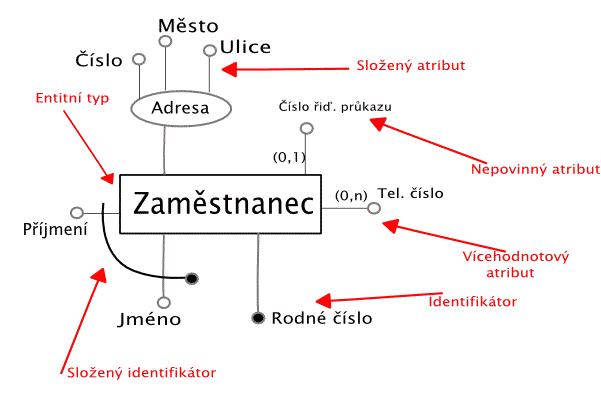
\includegraphics[width=14cm]{informatika/databazy/obrazky/er1.png}

(Entitní typ se všemožnými druhy atributů)
\end{center}
\end{obecne}

\begin{obecne}{Vztahový typ}
\emph{Vztahový typ} (v diagramu značený kosočtvercem) popisuje vztahy mezi jednotlivými entitami -- s těmi entitami, se kterými je v nějakém vztahu, je spojen čarou. Vztah může mít danou i \emph{kardinalitu} (kolik entit z každé strany do vztahu vstupuje), která může být typu $1:1$, $1:n$, $m:n$ a je značená vedle čáry spojující vztahový typ s entitou. Entity ve vztahu mohou mít navíc \emph{povinné či nepovinné členství} (vstupovat do něj vždy nebo jen někdy).

Vztahy mohou být buď binární nebo obecně $n$-ární, ale více než ternární vztahy se většinou neobjevují. Vztahy mohou být i rekurzivní, tj. do vztahů vstupují entity stejného typu. Instance vztahového typu je jednoznačně určena identifikátory instancí entit ve vztahu. Některé entitní typy mohou být spoluidentifikovány (nebo přímo identifikovány) vztahem -- pak se nazývají \emph{slabé entitní typy}.

\begin{center}
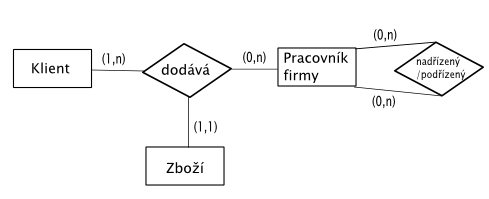
\includegraphics[width=12cm]{informatika/databazy/obrazky/er2.png}

(Vztahové typy)
\end{center}
Obrázek ukazuje ternární vztah s různými kardinalitami -- klientovi někdo dodává zboží jednou až $n$-krát, pracovník dodává nula až $n$-krát zboží (tj. jde o nepovinné členství ve vztahu, můžou existovat pracovníci, kteří nic nedodávají) a zboží je vždy někomu dodáváno právě jednou. Na zaměstnancích je zároveň ukázán rekurzivní binární vztah.


\begin{center}
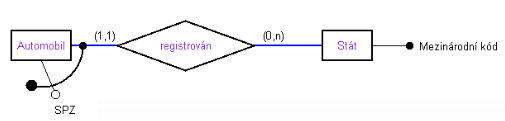
\includegraphics[width=10cm]{informatika/databazy/obrazky/er3.png}

(Slabý entitní typ. Zdroj: slidy Dr. T. Skopala k Databázovým systémům)
\end{center}
Tento obrázek ukazuje, jak vypadá slabý entitní typ -- automobil je identifikován svojí SPZ a zároveň státem, ve kterém je registrován.
\end{obecne}


\begin{obecne}{ISA hierarchie}
ISA hierarchie je rozšíření ER diagramů o \uv{dědičnost} entit -- tj. rozdělení entitních typů na subtypy (a přidání dalších vztahů nebo atributů pro subtypy). V ISA hierarchii se povoluje pouze jednonásobná dědičnost, navíc potomci nějakého entitního typu musí být jednoznačně identifikováni předkem (tj. všechny entity v hierarchii sdílí identifikátor).

\begin{center}
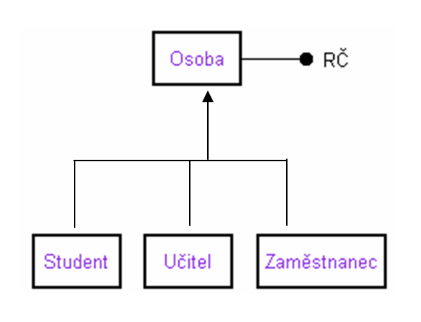
\includegraphics[width=6cm]{informatika/databazy/obrazky/er4.png}

(ISA hierarchie. Zdroj: slidy Dr. T. Skopala k Databázovým systémům)
\end{center}
\end{obecne}

\begin{obecne}{Úpravy ER diagramů}
V ER diagramu je možné provádět víceméně \uv{ekvivalentní} úpravy (výsledný diagram reprezentuje stejný koncept databáze), např. pro odstranění vztahů s kardinalitou $m:n$ (převod na dva vztahy kardinalitami $1:n$ a \emph{průnikový entitní typ}, který je vztahy určený, takže je slabý). Dalším důvodem úprav může být zbavení se ISA hierarchie. To se dá provést více způsoby, přičemž žádný z nich nefunguje úplně obecně:
\begin{pitemize}
    \item agregace atributů a vztahů potomka do předka a úprava kardinalit (převod na nepovinné atributy a nepovinné členství ve vztahu)
    \item odstranění předka a duplikace všech jeho atributů a vztahů v potomcích
    \item nahrazení ISA vztahu klasickým vztahem (z potomků vzniknou slabé entitní typy)
\end{pitemize}
Jiná úprava je odstranění vícehodnotového atributu -- převede se na vztah s kardinalitou $1:n$ a slabý entitní typ.
\end{obecne}

\begin{obecne}{Korektní ER schéma}
V \emph{korektním} ER schématu všechny entity a vztahy splňují:
\begin{pitemize}
    \item Žádný entitní typ nemá více než jednoho ISA předka.
    \item ISA vztahy netvoří orientovaný cyklus.
    \item Identifikační vztahy netvoří orientovaný cyklus.
    \item Potomek v ISA hierarchii není identifikačně závislý na žádném entitním typu (je již identifikován předkem).
    \item Jména entitních a vztahových typů jsou jednoznačná.
\end{pitemize}
\end{obecne}


TODO: Co je ksakru \uv{ metody návrhů IS}?

\subsection{SQL}

Zdroje: slidy z přednášek Databázové systémy a Databázové aplikace Dr. T. Skopala a Dr. M. Kopeckého.

\subsubsection*{Standardy SQL}

SQL (\emph{Structured query language}) je standardní jazyk pro přístup k relačním databázím (a dotazování nad nimi). Je zároveň jazykem pro definici dat (definition data language), vytváření a modifikace schémat (tabulek), manipulaci s daty (data manipulation language), vkládání, aktualizace, mazání dat, řízení transakcí, definici integritních omezení aj. Jeho syntaxe odráží snahu o co nejpřirozenější formulace požadavků -- je podobná anglickým \uv{větám}.

SQL je standard podle norem ANSI/ISO a existuje v několika (zpětně kompatibilních) verzích (označovaných podle roku uvedení):
\begin{description}
    \item[SQL 86] -- první \uv{nástřel}, průnik implementací SQL firmy IBM
    \item[SQL 89] -– malá revize motivovaná komerční sférou, mnoho detailů ponecháno implementaci
    \item[SQL 92] –- mnohem silnější a obsáhlejší jazyk. Zahrnuje už
    \begin{pitemize}
	\item modifikace schémat, tabulky s metadaty, 
	\item vnější spojení, množinové operace
	\item kaskádové mazání/aktualizace podle cizích klíčů, transakce
	\item kurzory, výjimky
    \end{pitemize}
    Standard existuje ve čtyřech verzích: Entry, Transitional, Intermediate a Full.
    \item[SQL 1999] -– přináší mnoho nových vlastností, např. 
    \begin{pitemize}	
	\item objektově-relační rozšíření
	\item nové datové typy -- reference, pole, full-text
	\item podpora pro externí datové soubory, multimédia
	\item triggery, role, programovací jazyk, regulární výrazy, rekurzivní dotazy ...
    \end{pitemize}
    \item[SQL 2003] -– další rozšíření, např. XML management
\end{description}

Komerční systémy implementují SQL podle různých norem, někdy jenom SQL-92 Entry, dnes nejčastěji SQL-99, ale nikdy úplně striktně. Některé věci chybí a naopak mají všechny spoustu nepřenositelných rozšíření -- např. specifická rozšíření pro procedurální, transakční a další funkcionalitu (T-SQL (Microsoft SQL Server), PL-SQL (Oracle) ). S novými verzemi se kompatibilita zlepšuje, často je možné používat obojí syntax. Přenos aplikace za běhu na jinou platformu je ale stále velice náročný -- a to tím náročnější, čím víc věcí mimo SQL-92 Entry obsahuje. Pro otestování, zda je špatně syntax SQL, nebo zda jen daná databázová platforma nepodporuje některý prvek, slouží SQL validátory (které testují SQL podle norem).


\subsubsection*{Dotazy v SQL}

Hlavním nástrojem dotazů v SQL je příkaz \texttt{SELECT}. Sdílí prvky relačního kalkulu i relační algebry -- obsahuje práci se sloupci, kvantifikátory a agregační funkce z relačního kalkulu a další operace -- projekce, selekce, spojení, množinové operace -- z relační algebry. Na rozdíl od striktní formulace relačního modelu databáze povoluje duplikátní řádky a NULLové hodnoty atributů.

Netříděný dotaz v SQL sestává z:
\begin{pitemize}
    \item příkazu(ů) \texttt{SELECT} (hlavní logika dotazování), to obsahuje vždy
    \item může obsahovat i množinové operace nad výsledky příkazů \texttt{SELECT} -- \texttt{UNION}, \texttt{INTERSECTION} ...
\end{pitemize}
Výsledky nemají definované uspořádání (resp. jejich pořadí je určeno implementací vyhodnocení dotazu).

Příkaz \texttt{SELECT} vypadá následovně (tato verze už zahrnuje i třídění výsledků):
\begin{verbatim}
SELECT [DISTINCT]
 výraz1 [[AS] c_alias1] [, ...]
FROM
 zdroj1 [[AS] t_alias1] [, ...]
[WHERE podmínka_ř]
[GROUP BY výraz_g1 [, …]
[HAVING podmínka_s]]
[ORDER BY výraz_o1 [, …] ASC/DESC]
\end{verbatim}
Kde
\begin{pitemize}
    \item výrazy mohou být sloupce, sloupce s agregačními funkcemi, výsledky dalších funkcí ...

\noindent \texttt{ výraz = <název sloupce>, <konstanta>, \\
 (DISTINCT) COUNT(~<název sloupce>~),\\
{}[DISTINCT] [~SUM~|~AVG~](~<výraz>~),\\
{}[~MIN~|~MAX~](~<výraz>~)}\\
a navíc lze použít operátory $+,-,*,/$.

    \item zdroje jsou tabulky nebo vnořené selecty
    \item výrazy i zdroje být přejmenovány pomocí \texttt{AS}, např. pro odkazování uvnitř dotazu nebo jména na výstupu (od SQL-92)
    \item podmínka je logická podmínka (spojovaná logickými spojkami \texttt{AND, OR}) na hodnoty dat ve zdrojích:

\texttt{podmínka = <výraz> BETWEEN <x> AND <y>, <výraz> LIKE "\%\_ ... ",\\
<výraz> IS [NOT] NULL,\\
<výraz> > = <> <= < > [<výraz>/ ALL / ANY <dotaz>],\\
<výraz> NOT IN [<seznam hodnot> / <dotaz>], EXIST ( <dotaz> )}

    \item \texttt{GROUP BY} znamená agregaci podle unikátních hodnot jmenovaných sloupců (v ostatních sloupcích vznikají množiny hodnot, které se spolu s oněmi unikátnímí vyskytují na stejných řádkách
    \item \texttt{HAVING} označuje podmínku na agregaci
    \item \texttt{ORDER BY} definuje, podle hodnot ve kterých sloupcích nebo podle kterých jiných výrazů nad nimi provedených se má výsledek setřídit (\texttt{ASC} požaduje vzestupné setřídění, \texttt{DESC} sestupné).
\end{pitemize}

SQL nemá příkaz na omezení rozsahu na některé řádky (jako např. \uv{potřebuji jen 50.-100. řádek výpisu}), a to lze řešit buď složitě standardně (počítání kolik hodnot je menších než vybraná, navíc náročné na hardware) nebo pomocí některého nepřenositelného rozšíření.

\medskip\noindent
Pořadí vyhodnocování jednoho příkazu \texttt{SELECT} (nebereme v úvahu optimalizace):
\begin{penumerate}
    \item Nejprve se zkombinují data ze všech zdrojů (tabulek, pohledů, poddotazů). Pokud jsou odděleny čárkami, provede se kartézský součin (to samé co \texttt{CROSS JOIN}), v SQL-92 a vyšším i složitější spojení -- \texttt{JOIN ON} (vnitřní spojení podle podmínky), \texttt{NATURAL JOIN} (\uv{přirozené} spojení podle stejných hodnot stejně pojmenovaných sloupců), \texttt{OUTER JOIN} (\uv{vnější} spojení, do kterého jsou zahrnuty i záznamy, pro které v jednom ze zdrojů není nalezeno nic, co by odpovídalo podmínce, doplněnné NULLovými hodnotami) atd.
    \item Vyřadí se vzniklé řádky, které nevyhovují podmínce (\texttt{WHERE})
    \item Zbylé řádky se seskupí do skupin se stejnými hodnotami uvedených výrazů (\texttt{GROUP BY}), každá skupina obsahuje atomické sloupce s hodnotami uvedených výrazů a množinové sloupce se skupinami ostatních hodnot sloupců.
    \item Vyřadí se skupiny, nevyhovující podmínce (\texttt{HAVING})
    \item Výsledky se setřídí podle požadavků
    \item Vygeneruje se výstup s požadovanými hodnotami
    \item V případě \texttt{DISTINCT} se vyřadí duplicitní řádky
\end{penumerate}


\begin{poznamka}
\begin{pitemize}
    \item Klauzule \texttt{GROUP BY} setřídí před vytvořením skupin všechny řádky dle výrazů v klauzuli. Proto by se měl seskupovat co nejmenší možný počet řádek. Pokud je možné řádky odfiltrovat pomocí WHERE, je výsledek efektivnější, než následné odstraňování celých skupin.
    \item  Klauzule \texttt{DISTINCT} třídí výsledné záznamy (před operací ORDER BY), aby našla duplicitní záznamy. Pokud to jde, je vhodné se bez ní obejít.
    \item Klauzule \texttt{ORDER BY} by měla být použita jen v nutných případech. Není příliš vhodné ji používat v definicích pohledů, nad kterými se dále dělají další dotazy.
\end{pitemize}
\end{poznamka}


\subsubsection*{Definice a manipulace s daty, ostatní příkazy}

Standard SQL podporuje několik druhů datových typů:
\begin{pitemize}
    \item textové v národní a globální (UTF) znakové sadě (několika druhů -- proměnné a pevné délky): \texttt{CHARACTER(n)}, \texttt{NCHAR(n)},
    \texttt{CHAR VARYING(n)}
    \item číselné typy -- \texttt{ NUMERIC(p[,s]), INTEGER, INT, SMALLINT,\\  FLOAT(presnost), REAL, DOUBLE PRECISION}
    \item datumové typy -- \texttt{DATE, TIME, TIMESTAMP, TIMESTAMP(presnost\_sekund) WITH TIMEZONE}
\end{pitemize}
Databázové servery ne vždy podporují všechny uvedené typy. Nemusí je podporovat nativně, někdy si pouze \uv{přeloží} název typu na podobný nativně podporovaný typ.

\medskip
\begin{obecne}{Příkaz \texttt{CREATE TABLE}}
Tento příkaz slouží k vytvoření nové tabulky. Je nutné definovat její název, atributy a jejich domény (datové typy); dále je možné definovat integritní omezení (klíče, cizí klíče, odkazy, podmínky). Příkaz vypadá následovně:
\begin{center}
\texttt{CREATE TABLE <název> <def. sloupce/i.o. tabulky, ...> }
\end{center}
A uvnitř potom
\begin{verbatim}
def. sloupce = <název> <dat.typ> 
    [DEFAULT NULL|<hodnota>] [<i.o.sloupce>] 
dat.typ = [VARCHAR(n) | BIT(n) | INTEGER | FLOAT | DECIMAL ...] 
i.o.sloupce = [CONSTRAINT <jméno>] [NOT NULL / UNIQUE / PRIMARY KEY], 
    REFERERENCES <tabulka>(<sloupec>) <akce>, CHECK <podmínka> 
akce = [ON UPDATE / ON DELETE] 
    [CASCADE / SET NULL / SET DEFAULT / NO ACTION(hlášení chyby) ] 
i.o.tabulky = UNIQUE, PRIMARY KEY <sloupec, ... >, 
    FOREIGN KEY <sloupec, ... >, 
    REFERENCES <tabulka>(<sloupec, ... >), 
    CHECK( <podmínka> )
\end{verbatim}
\end{obecne}

\medskip
\begin{obecne}{Příkazy pro manipulaci se schématem}
\begin{pitemize}
    \item Úprava tabulky:
\begin{verbatim}
ALTER TABLE <název> ADD {COLUMN} <def.sloupce>, ADD <i.o.tabulky>, 
    ALTER COLUMN <sloupec> [ SET / DROP ], DROP COLUMN <sloupec>, 
    DROP CONSTRAINT <jméno i.o.> 
\end{verbatim}
    \item Smazání tabulky (není to samé jako vymazání všech dat z tabulky!):
\begin{verbatim}
DROP TABLE <tabulka> 
\end{verbatim}
    \item Vytvoření \uv{pohledu} -- navenek se chová jako tabulka, ale vnitřně se při každém dotazu provede vnořený dotaz (který definicí pohledu zapisuji):
\begin{verbatim}
CREATE VIEW <název "tabulky"> ( <sloupec, ... > ) 
    AS <dotaz> {WITH [ LOCAL / CASCADED ] CHECK OPTION }
\end{verbatim}
    Některé databázové platformy umožňují do takto vytvořených pohledů i zapisovat.
\end{pitemize}
\end{obecne}

\medskip
\begin{obecne}{Příkazy pro manipulaci s daty}
\begin{pitemize}
    \item Vložení nových dat do tabulky
\begin{verbatim}
INSERT INTO <tabulka> ( <sloupec, ... > ) 
    [VALUES ( <výraz, ... > ) / (<dotaz>) ] 
\end{verbatim}
    \item Úprava dat (na řádcích které vyhovují podmínce se nastaví zadané hodnoty vybraným sloupcům):
\begin{verbatim}
UPDATE <tabulka> SET 
    ( <sloupec> = [ NULL / <výraz> / <dotaz> ] , ... ) 
    WHERE (<podmínka>) 
\end{verbatim}
    \item Smazání řádků vyhovujících podmínce z tabulky:
\begin{verbatim}
DELETE FROM <tabulka> ( WHERE <podmínka> ) 
\end{verbatim}
\end{pitemize}
\end{obecne}

TODO: doplnit ?

\subsection{Indexy, triggery, uložené procedury, uživatelé}

TODO: pořádná definice indexu

\begin{obecne}{Index}
Index je obvykle definován výběrem tabulky a jejího konkrétního sloupce (nebo sloupců), nad kterými si designér databáze přeje dotazování urychlit; dále pak technickým určením typu. Chování a způsoby uložení indexů se mohou významně lišit podle použité databázové technologie.
Výjimku mohou tvořit například full-textové indexy, které jsou v některých případech (nerelační databáze typu Lotus Notes) definovány nad celou databází, nikoliv nad konkrétní tabulkou. 
\end{obecne}

\begin{obecne}{Použití indexu}
Na první pohled by se mohlo zdát, že čím víc indexů, tím lepší chování databáze a že po vytvoření indexů pro všechny sloupce všech tabulkách dosáhneme maximálního zrychlení. Tento přístup naráží bohužel na dva zásadní problémy: 
\begin{penumerate}
    \item Každý index zabírá v paměti vyhrazené pro databázi nezanedbatelné množství místa (vzhledem k paměti vyhrazené pro tabulku). Při existenci mnoha indexů se může stát, že paměť zabraná pro jejich chod je skoro stejně velká, jako paměť zabraná jejími daty - zvláště u rozsáhlých tabulek (typu faktových tabulek v datovém skladu) může něco takového být nepřijatelné. 
    \item Každý index zpomaluje operace, které mění obsah indexovaných sloupců (například SQL příkazy UPDATE, INSERT). To je dáno tím, že databáze se v případě takové operace nad indexovaným sloupcem musí postarat nejen o změny v datech tabulky, ale i o změny v datech indexu. 
\end{penumerate}
\end{obecne}

\begin{obecne}{Typy indexů}
Indexy mohou mít svůj typ, který blíže určuje, jakým způsobem má být přistupování k datům tabulky optimalizováno. Označení se různí, ale nejčastěji je to:
\begin{pitemize}
    \item PRIMARY - Tento typ se v každé tabulce může vyskytovat nejvýše jednou. Definuje sloupec tabulky, který svou hodnotou jednoznačně identifikuje záznam. Ve většině případů se dodržuje konvence takový sloupec nazvat ID a jeho datový typ stanovit jako celé číslo (není-li potřeba jinak). Databázový server by měl být schopen nedopustit, aby byla do sloupce, k němuž se tento typ indexu vztahuje, byla vložena hodnota, která již v tabulce existuje (většinou takový pokus končí chybovou hláškou). 
    \item UNIQUE - Tento typ je podobný PRIMARY co do jednoznačnosti záznamu v tabulce (jak naznačuje i jeho název) a dopadu, který to na práci s databází má; ale může se vyskytovat u více sloupců tabulky. Podle účelu, ke kterému má tabulka sloužit, se občas definují indexy složené z více sloupců - potom opět nelze vložit záznam, který by již v této kombinaci někde v tabulce existoval. 
    \item INDEX - Definicí indexu tohoto typu je v tabulce zajištěna optimalizace vyhledávání podle sloupce, ke kterému se daný index váže. Většinou si databázový server vytvoří a nadále udržuje vnitřní seznam odkazů na řádky tabulky, seřazený podle hodnot sloupce, k němuž se váže. Udržování takto seřazené posloupnosti urychluje vyhledávání (je možno použít některé interpolační numerické metody), řazení i jiné zásahy do tabulky, které jsou omezeny podmínkou na dotyčné záznamy. 
    \item FULL-TEXT - Vytvořením tohoto indexu se databázový server bude snažit optimalizovat full-textové vyhledávání v daném sloupci u dané tabulky.
\end{pitemize}
\end{obecne}

\begin{obecne}{Triggery}
  Databázový trigger je programový kód, který je automaticky vykonán jako
  reakce na nějakou událost v určité databázové tabulce. Triggery mohou omezit
  přístup k určitým datům, provádět logování, nebo kontrolovat změny dat.

  Rozlišujeme dvě hlavní třídy triggerů a to \emph{řádkový trigger} a
  \emph{dotazový (statement) trigger}. Řádkový trigger můžeme definovat pro
  každý řádek tabulky, zatímco dotazový trigger se vykoná pouze jednou pro
  konkrétní databázový dotaz. Každá třída triggerů může být několika typů. Jsou
  \emph{before triggers} a \emph{after triggers}, což značí kdy má být trigger
  vykonán. Také se můžeme setkat s \emph{instead of triggers}, který je potom
  vykonán \emph{místo} dotazu kterým byl spuštěn. 

  Jaké události mohou trigger spustit se pochopitelně liší databázový systém od
  systému, ale existují tři typické události, které to mohou být:
  \begin{penumerate}
    \item INSERT~-- nový záznam je vložen do databáze,
    \item UPDATE~-- záznam je měněn,
    \item DELETE~-- záznam je mazán.
  \end{penumerate}
  Kromě těchto typických událostí může databázový systém umožňovat nastavovat
  triggery také na mazání, či vytváření celých tabulek, či dokonce přihlášení
  nebo odhlášení uživatele.

  Hlavní vlastnosti a efekty databázových triggerů jsou:
  \begin{pitemize}
    \item nepřijímají žádné parametry nebo argumenty,
    \item nemohou volat operace pro řízení transakcí COMMIT a ROLLBACK,
    \item mají přístup k datům, které budou měněny, je tedy možné vykonávat akce
    na základě nich,
    \item nemohou vracet záznamy,
    \item obtížně se ladí,
    \item mnoho triggerů nebo složité triggery mohou práci s databází velice
    zpomalit a navíc znepřehlednit.
  \end{pitemize}
\end{obecne}

\begin{obecne}{K čemu triggery používat?}
  Triggery se v databázích používají z několika důvodů, které mohou souviset s
  konzistencí dat, jejich údržbou, nebo mohou být způsob, kterým databáze
  komunikuje s okolím. Podívejme se na některá typická schémata:
  \begin{pitemize}
    \item \textbf{Konzistence dat}~-- Trigger může provést výpočet a na základě
    toho povolit nebo nepovolit změnu dat v databázi. Například trigger může zakázat
    smazání zákazníka z databáze v případě, kdy má u nás nějaký dluh a podobně.  
    \item \textbf{Logování}~-- Trigger může evidovat kdo, kdy a jak měnil data.
    Lze tak dohledat pracovníka, který zadal špatné údaje nebo zjistit, v kolik
    hodin došlo k včerejší uzávěrce.
    \item \textbf{Verzování dat}~-- Díky triggerům lze snadno naprogramovat
    aplikaci tak, aby jedna tabulka udržovala historii změn tabulky jiné. To lze
    s úspěchem použít třeba jako bezpečnostní mechanismus. 
    \item \textbf{Zasílání zpráv}~-- Trigger může spustit nějaký externí
    program nebo proces. Například může trigger autorovi poslat e-mail,
    pokud byl k jeho článku přidán příspěvek.
  \end{pitemize}
\end{obecne}

\begin{obecne}{Uložené procedury}
  Uložená procedura (anglicky stored procedure) je databázový objekt, který
  neobsahuje data, ale část programu, který se nad daty v databázi má vykonávat.

  Uložená procedura je především procedura. Jedná se o část programu, který je
  (nebo by aspoň měl být) jasně funkčně oddělený od svého okolí, má interface
  (seznam parametrů) pro komunikaci s jinými moduly programu. Může mít vlastní
  lokální proměnné neviditelné pro ostatní části programu. 

  Uložená procedura je uložená (rozuměj: uložená v databázi). To znamená, že se k
  ní lze chovat stejně jako ke každému jinému objektu databáze (indexu, pohledu,
  triggeru apod.). Lze jí založit, upravovat a smazat pomocí příkazů dotazovacího
  jazyka databáze (v případě relační databáze obvykle pomocí příkazů DDL SQL). 

  Pro psaní uložených procedur je obvykle používán specifický jazyk konkrétní
  databáze, který je rozšířením jejího dotazovacího jazyka (hezkým příkladem je
  databáze Oracle s procedurálním jazykem PL/SQL, který je rozšířením klasického
  dotazovacího jazyka SQL).
\end{obecne}

\begin{obecne}{Proč ukládat procedury?}
  \begin{pitemize}
      \item \textbf{Jednotné rozhraní}~-- Použití uložených procedur vychází z
      faktu, že většina operací nad daty v databázi probíhá stejně bez ohledu na
      to, kdo operaci provádí. Příklad: Pokud je třeba uložit do tabulky
      zákazníků nového zákazníka, tak se to z pohledu databáze děje stejně pro
      zákazníka internetového obchodu, pro zákazníka, kterého zadává pracovnice
      telefonického centra přes formulář programu napsaného například v C++ ,
      nebo pro zákazníky, kteří jsou vkládáni automaticky na základě textového
      reportu, který přijde každý den z \uv{kamenných} prodejních míst a je
      zpracováván pomocí programu napsaného v PowerBuilderu. Je tedy celkem
      dobrý důvod, aby existovala uložená procedura \uv{Zapiš nového zákazníka},
      kterou by mohly volat všechny tři výše uvedené aplikace - alternativou bez
      uložené procedury by bylo, že bych podobnou proceduru musel napsat ve
      třech verzích - jednou v C++, jednou v Power Builderu a jednou v rámci
      programu pro internetový obchod (třeba ASP nebo PHP). 
      \item \textbf{Skrytí datových operací}~-- Druhou výhodou použití uložených
      procedur je, že se nemusím (v programu na \uv{klientské} straně) zabývat
      tím, jak jsou data uložena v konkrétních tabulkách. V našem případě je mi
      jedno, jak si databáze uvnitř pamatuje zákazníky - prostě zadám jako
      parametr procedury jméno, příjmení, číslo kreditky a co si zákazník koupil
      - a databáze (resp. její uložená procedura) si to nějak přebere. Uložené
      procedury se v případě databázových aplikací staly základním kamenem pro
      realizaci architektury klient/server, kdy je na jedné straně (klientská
      část) realizována v běžném procedurálním programovacím jazyku komunikace s
      uživatelem (formuláře nebo třeba webové stránky) a na druhé straně
      (serverová část) je pomocí uložených procedur realizována správa dat v
      relační databázi. Obě části (klientská a serverová) mezi sebou komunikují
      přes co nejjednodušší rozhraní - voláním uložených procedur. 
  \end{pitemize}
\end{obecne}

TODO: uživatelé

\subsection{Vícevrstevné architektury}

TODO: předělat, tohle je jen copy \& paste z Wiki a slajdů VUT Brno


\begin{obecne}{Multitier architecture}
Multi-tier architecture (often referred to as n-tier architecture) is a client-server architecture, originally designed by Jonathon Bolster of Hematites Corp, in which an application is executed by more than one distinct software agent. For example, an application that uses middleware to service data requests between a user and a database employs multi-tier architecture. The most widespread use of "multi-tier architecture" refers to three-tier architecture
\end{obecne}


\begin{obecne}{Základ kooperativního zpracování}
Faktory ovlivňující architekturu:
\begin{pitemize}
\item požadavky na interoperabilitu zdrojů 
\item růst velikosti zdrojů 
\item růst počtu klientů 
\end{pitemize}
Typy služeb v databázové technologii:
\begin{pitemize}
\item prezentační služby: příjem vstupu, zobrazování výsledků 
\item prezentační logika: řízení interakce (hierarchie menu, obrazovek)
\item logika aplikace: operace realizující algoritmus aplikace
\item logika dat: podpora operací s daty (integritní omezení, ...)
\item datové služby: akce s databází (definice a manipulace, transakční zpracování, ...) 
\item služby ovládání souborů: vlastní V/V operace
\end{pitemize}
\end{obecne}

\begin{obecne}{Varianty architektury klient-server}
\begin{pitemize}
    \item \textbf{Klient-server se vzdálenými daty} \\
Na serveru jsou jen datové služby a ovládání souborů, zbytek zajišťují klienti. Problémem jsou velké nároky na přenosovu kapacitu od klienta k serveru a HW zatížení klientských stanic
    \item \textbf{Klient-server se vzdálenou prezentací} \\
Na klientské stanici jsou jen prezentační služby a prezentační logika, zbytek je na serveru. Nevýhodou je právě zátěž na HW serveru.
    \item \textbf{Klient-server s rozdělenou logikou} \\
Část logiky aplikací i logiky dat je na serveru a část zpracovává klient. Jde o vyvážené řešení, které má ale horší rozšířitelnost.
    \item \textbf{Třívrstvá architektura} \\
Zahrnuje dva servery -- aplikační a databázový, spojené rychlou linkou. Z hlediska zátěže a rozšířitelnosti nejvýhodnější.
\end{pitemize}
\end{obecne}

\begin{obecne}{Přínos architektury klient/server a třívrstvé architektury}
\begin{pitemize}
 \item pružnější rozdělení práce \item lze použít horizontální(více serverů) i vertikální(výkonnější server) škálování \item aplikace mohou běžet na levnějších zařízeních \item na klientských stanicích lze používat oblíbený prezentační software \item standardizovaný přístup umožňuje zpřístupnit další zdroje \item centralizace dat podporuje účinnější ochranu \item u třívrstvé architektury centralizace údržby aplikace, možnost využití sdílených objektů (business objects) několika aplikacemi
\end{pitemize}
\end{obecne}

\begin{obecne}{Podpora pro rozdělení zátěže v architektuře klient/server}
\begin{pitemize}
 \item deklarativní integritní omezení \item databázové triggery \item uložené podprogramy
\end{pitemize}
\end{obecne}


\begin{obecne}{Three-tier architecture}
'Three-tier' is a client-server architecture in which the user interface, functional process logic ("business rules"), data storage and data access are developed and maintained as independent modules, most often on separate platforms. The term "three-tier" or "three-layer", as well as the concept of multitier architectures, seems to have originated within Rational Software.

The three-tier model is considered to be a software architecture and a software design pattern.

Apart from the usual advantages of modular software with well defined interfaces, the three-tier architecture is intended to allow any of the three tiers to be upgraded or replaced independently as requirements or technology change. For example, a change of operating system from Microsoft Windows to Unix would only affect the user interface code.

Typically, the user interface runs on a desktop PC or workstation and uses a standard graphical user interface, functional process logic may consist of one or more separate modules running on a workstation or application server, and an RDBMS on a database server or mainframe contains the data storage logic. The middle tier may be multi-tiered itself (in which case the overall architecture is called an "n-tier architecture").

The 3-Tier architecture has the following 3-tiers:
\begin{pitemize}
    \item Presentation Tier
    \item Application Tier/Logic Tier/Business Logic Tier
    \item Data Tier
\end{pitemize}
\end{obecne}


\begin{obecne}{Web Development usage}

In the Web development field, three-tier is often used to refer to Websites, commonly Electronic commerce websites, which are built using three tiers:
\begin{pitemize}
    \item A front end Web server serving static content
    \item A middle dynamic content processing and generation level Application server, for example Java EE platform.
    \item A back end Database, comprising both data sets and the Database management system or RDBMS software that manages and provides access to the data.
\end{pitemize}
\end{obecne}

\begin{obecne}{Other Considerations}

To further confuse issues, the particular data transfer method between the 3 tiers must also be considered. The data exchange may be file-based, client-server, event-based, etc. Protocols involved may include one or more of SNMP, CORBA, Java RMI, Sockets, UDP, or other proprietary combinations/permutations of the above types and others. Typically a single "middle-ware" implementation of a single protocol is chosen as the "standard" within a given system, such as J2EE (which is Java specific) or CORBA (which is language/OS neutral.) The importance of the decision of which protocol is chosen affects such issues as the ability to include legacy applications/libraries, performance, maintainability, etc. When choosing a "middle-ware protocol" (not to be confused with the "middle-of-the-three-tiers") engineers should not be swayed by "public opinion" about a protocol's modern-ness, but should consider the technical benefits and suitability to solve a problem. (for example CGI is very old and "out of date" but is still quite useful and powerful, so is shell scripting, and UDP for that matter)

Ideally the high-level system abstract design is based on business rules and not on the front-end/back-end technologies. The tiers should be populated with functionality in such a way as to minimize dependencies, and isolate functionalities in a coherent manner - knowing that everything is likely to change, and changes should be made in the fewest number of places, and be testable.
\end{obecne}

\subsection{Vazba databází na internetové technologie}

TODO: všechno


\subsection{Organizace dat na vnější paměti, B-stromy a jejich varianty}


\subsubsection*{Vnější paměť}

\begin{definiceN}{Vnější paměť}
\emph{Vnější paměť} je úložiště dat (paměťové médium), u kterého je rychlost načítání dat zpravidla nízká a přístup k nim ne úplně přímý (záleží na uspořádání dat na médiu), ne-li pouze sekvenční (oproti vnitřní paměti s rychlým náhodným přístupem a menší kapacitou). Příkladem vnější paměti je pevný disk nebo magnetická páska.

\emph{Magnetické pásky} poskytují vysokou kapacitu, ale nízkou rychlost a pouze sekvenční přístup. Pro jejich kapacitu je důležitá hustota záznamu, potřebují meziblokové mezery pro vyrovnání nepřesnosti přetáčení pásky.

\emph{Pevné disky} umožňují přímý přístup, ale jeho rychlost není vždy stejná. Ovlivňuje ji fyzická vzdálenost dat -- pevný disk má několik \emph{válců}, na nichž jsou uloženy jednotlivé datové \emph{stopy}. K válcům přísluší \emph{čtecí hlavy} (je jich stejně jako válců, ale pohybují se všechny současně, takže může v 1 okamžiku číst jen jedna). Disky jsou většinou rozděleny na \emph{sektory} -- nejmenší jednotku dat, kterou je možné načíst nebo uložit (zpravidla jednotky KB). Pro rychlost přístupu k datům jsou důležité tyto veličiny (výrobcem disků jsou zpravidla udávány průměrné hodnoty):
\begin{pitemize}
    \item \emph{seek} ($s$) -- přesun na jinou stopu, dnes zpravidla kolem 4-8~ms
    \item \emph{(average) rotational delay} ($r$) -- otočení válců -- 1 půlotáčka, pro nejčastější 7200rpm disk je to cca 4~ms
    \item \emph{block transfer time} ($btt$) -- doba přenesení 1 bloku po sběrnici, na ATA/100 disku se 4~KB bloky teoreticky 0.04~ms
\end{pitemize}
Pokud jsou data umístěna na disku za sebou sekvenčně, rychlost jejich načtení je mnohem vyšší než při náhodném rozmístění, protože není třeba provádět přesuny mezi stopami a otáčení válců navíc.
\end{definiceN}

\begin{priklad}
\emph{Jak vypadá načtení 1~MB dat z pevného disku?} Předpokládejme, že na 1 stopu se vejde 512~KB a 1 blok má 4~KB. Jsou-li data umístěna na disku sekvenčně, potřebuji pro načtení 1~MB dat najít první blok a potom číst dvě celé stopy (2 otáčky), tj. celkem $s+r+(2\cdot2r)$ (a přenos po sběrnici lze zanedbat, protože probíhá zároveň se čtením). Pokud jsou data na disku náhodně rozprostřena, potřebuji celkem 256-krát najít blok a načíst ho: $256\cdot(s+r+btt)$, takže operace trvá až 100-krát déle.
\end{priklad}


\subsubsection*{Soubor}

\begin{definiceN}{Záznam, klíč}
\emph{(Logický) záznam} je jednotka dat (např. v databázi), má \emph{atributy} (z nichž každý má jméno a doménu -- povolenou množinu hodnot). Logickému záznamu v reprezentaci na disku odpovídá \emph{fyzický záznam} (nějaké délky $R$ -- pevné nebo proměnné), který navíc může obsahovat ještě další data -- oddělovače, ukazatele, hlavičky. 

\emph{Klíč} je množina atributů, která jednoznačně identifikuje záznam; proti tomu \emph{vyhledávací klíč} je množina atributů, pro kterou lze nalézt množinu odpovídajících záznamů. Vyhledávací klíče jsou tří druhů: hodnotový (\uv{obyčejné} hodnoty některých atributů), hašovaný a relativní (přímo pozice v souboru).
\end{definiceN}

\begin{definiceN}{Soubor}
(Homogenní) \emph{soubor} je multimnožina záznamů. Fyzicky na vnější paměti je organizován do \emph{bloků (stránek)} (velikosti $B$, typicky několika KB) -- hl. jednotkou přenosu dat mezi vnitřní a vnější pamětí. Poměr velikosti záznamu k velikosti bloku ($B/R$) se nazývá \emph{blokovací faktor} ($\lfloor b\rfloor$). Záznamy mohou být rozprostřeny i přes několik stránek, nebo může být pouze jeden záznam na 1 stránku; ideální (ale ne vždy dosažitelné) je, pokud beze zbytku zaplňují stránky. Na souboru jsou definovány operace se záznamy: \emph{insert, delete, update} a \emph{fetch}.
\end{definiceN}

\begin{definiceN}{Dotaz}
\emph{Dotaz} je každá funkce, která každému svému argumentu přiřadí odpovídající množinu záznamů ze souboru (\uv{totální vyčíslitelná funkce definovaná na souboru}). Dotazy mohou být těchto typů:
\begin{pitemize}
    \item Načtení všech záznamů ({\tt SELECT * FROM tabulka})
    \item Na úplnou shodu ({\tt SELECT * FROM tabulka WHERE sloupec1 = 'hodnota' AND sloupec2 = 'hodnota'} pro tabulku se 2 sloupci -- dány jsou všechny atributy)
    \item Na částečnou shodu\\({\tt SELECT * FROM tabulka WHERE sloupec1 = 'hodnota'} pro tabulku se 2 sloupci -- zadaná je jen část atributů)
    \item Na intervalovou shodu (částečnou nebo úplnou) ({\tt SELECT * FROM tabulka WHERE sloupec1 > 'hodnota'})
\end{pitemize}
U souborů se sleduje rychlost provedení těchto operací.
\end{definiceN}


\subsubsection*{Statické metody organizace souboru}

\begin{definiceN}{Schéma organizace souboru}
\emph{Schéma organizace souboru} je popis logické paměťové struktury, do níž lze zobrazit logický soubor, spolu s algoritmy operací nad touto strukturou. Ta je obvykle tvořena z logických stránek (bloků pevné délky) a může popisovat více provázaných log. souborů, z nichž \emph{primární soubor} je ten, který obsahuje uživatelská data. Operace definované nad schématem org. souboru jsou kromě operací nad soubory ještě \emph{build, reorganization, open} a \emph{close}.

Proti němu stojí \emph{fyzické schéma souboru} -- struktura nad fyzickými soubory, nejblíže hardwaru je \emph{implementační schéma souboru}.

Zajištění \emph{Vyváženosti struktury} znamená zajištění omezení cesty při vyhledávání nějakým výrazem (zaručení asymptotické složitosti), navíc zaručení rovnoměrnosti zaplnění struktury -- \emph{faktor naplnění stránek}. Schémata, která splňují obě podmínky, se nazývají \emph{dynamická}, ostatní jsou označována jako \emph{statická}.
\end{definiceN}

\begin{poznamkaN}{Časové odhady}
Pro schémata organizace souborů se počítají časové odhady provedení jednotlivých operací -- jednodušších, jako je přístup k záznamu ($T_F$), \emph{rewrite} -- přepis během 1 otáčky disku ($T_{RW}$), příp. sekvenční čtení; dále i složitějších jako vyhledání záznamu, přidání, smazání a úprava záznamu, reorganizace struktury nebo načtení celého souboru.
\end{poznamkaN}

\begin{obecne}{Hromada (neuspořádaný sekvenční soubor)}
\emph{Hromada(heap)} je naprosto nejjednodušší schéma organizace souboru, kdy jsou záznamy v souboru jen náhodně seřazeny za sebou. Časová složitost vyhledávání je $O(n)$, pokud $n$ je počet záznamů. Jde o \emph{nehomogenní soubor}, kde záznamy obvykle nemají pevnou délku. 
\end{obecne}

\begin{obecne}{Uspořádaný sekvenční soubor}
V \emph{uspořádaném sekvenčním souboru} jsou záznamy řazeny podle klíče. Aktualizované záznamy se umístí do zvláštního souboru a až při další operaci \uv{reorganization} jsou přidány do primárního. Složitost nalezení záznamu je také $O(n)$, ale pokud se hledá podle klíče, podle kterého jsou záznamy seřazeny, a navíc je soubor na médiu s přímým přístupem, sníží se na $O(\log n)$.
\end{obecne}

\begin{obecne}{Index-sekvenční soubor}
Toto schéma uvažuje primární soubor jako sekvenční, uspořádaný podle primárního klíče. Nad ním je pak vytvořen (třeba i víceúrovňový) \emph{index}. Ten sestává ze seznamu čísel stránek a minimálních hodnot klíče jim odpovídajících záznamů. Pokud má index víc úrovní, provádí se pro vyšší úrovně to samé na blocích indexů úrovně o 1 nižší. Nejvyšší úroveň indexu se obvykle vejde do 1 bloku, tzv. \emph{master}. 

Počet potřebných úrovní pro $n$ záznamů se dá spočítat jako $\lceil\log_p\frac{n}{\lfloor b\rfloor}\rceil$, kde $p=\lfloor\frac{B}{V+P}\rfloor$ při velikosti klíče $V$ a pointeru na stránku $P$. Problémem je přidávání nových záznamů, kdy se tyto řetězí za sebe v tzv. \emph{oblasti přetečení} (každý z nich má pointer na další záznam v oblasti přetečení). Pro oddálení nutnosti vkládání do oblasti přetečení lze iniciálně bloky plnit na méně než 100\%.
\end{obecne}


\begin{obecne}{Indexovaný soubor}
\emph{Indexovaný soubor} znamená primární soubor plus indexy pro různé vyhledávací klíče. Neindexují se už stránky, ale přímo záznamy, a proto primární soubor nemusí být nutně setříděný. Index může být podobný jako u index-sekvenčního souboru, pro záznamy se stejným klíčem je ale vhodné, aby byly na všech úrovních indexu kromě poslední sloučené. Při aktualizaci se nepoužívá oblast přetečení, mění se pouze index.

Existuje i několik dalších variant indexů. Pro zmenšení náročnosti dotazů na kombinovanou částečnou shodu se používá \emph{kombinovaný index} pro více atributů, u něhož je ale nutné předem zjistit na které kombinace atributů budou často pokládány dotazy, a pro takové kombinace tento index teprve vytvořit. \emph{Clusterovaný index} zaručuje, že záznamy s podobnou hodnotou indexovaného atributu jsou blízko sebe v primárním souboru -- např. pokud je primární soubor podle tohoto atributu setříděny. Tento index lze použít jen pro 1 atribut. 

\emph{Bitové mapy} se dají použít jako index pro atributy s malou doménou (množinou možných hodnot) -- pro každou hodnotu této domény se vyrobí vektor bitů stejné délky, jako je počet záznamu v primárním souboru, kde jednička na $i$-té pozici indikuje, že $i$-tý záznam má právě tuto hodnotu atributu. To umožňuje jednoduché provádění booleovských dotazů na tento atribut. Vektory bitů navíc lze komprimovat, takže nezabírají tolik místa.
\end{obecne}

\begin{obecne}{Soubor s přímým přístupem}
V tomto schématu jsou záznamy v primárním souboru (\uv{adresovém prostoru} velikosti $M$) rozptýleny pomocí \emph{hashovací funkce}. Často se používá funkce $h=k\mod M'$, kde $M'$ je nejbližší prvočíslo menší než velikost adresového prostoru. Hashovací funkcí se určuje buď jenom číslo stránky, nebo i relativní pozice v ní. Při hashování vznikají kolize, které se dají řešit \emph{otevřeným adresováním} (řetězením kolizních záznamů za sebe), \emph{rehashováním} (další funkcí) nebo použitím \emph{oblasti přetečení}. Snaha je většinou umístit kolizní záznamy do stejné stránky. 

Pokud je hashovací funkce prostá, jedná se o \emph{perfektní hashování}. Toho ale v praxi vlastně nelze dosáhnout, takže se tento výraz používá i pro označení stavu, kdy je pro nalezení záznamu potřeba nejvýš $O(1)$ přístupů k médiu. Očekávaná délka řetězce kolizí při počtu $N$ záznamů v prostoru velikosti $M$ je $1/(1-\frac{N}{M})$.
\end{obecne}

\subsubsection*{Třídění na vnější paměti}

\begin{algoritmusN}{Třídění sléváním (Mergesort)}
Tento algoritmus se používá pro třídění dat, která se nevejdou do vnitřní paměti. Dá se použít i při sekvenčním přístupu k datovým souborům. Nejjednodušší verze bez bufferů vypadá takto:
\begin{pitemize}
    \item inicializace: na začátku každého kroku data rozdělí do 2 souborů
    \item načte 2 záznamy, každý z jednoho souboru a porovná je
    \item ve správném pořadí je zapíše do výstupního souboru, ze vstupního souboru si načte další dva
    \item v prvním kroku získám uspořádané posloupnosti délky 2; v dalších krocích vždy porovnám načtené prvky, zapíšu menší z nich a ze souboru odkud tento pocházel si načtu další, takže získám vždy uspořádané posloupnosti dvojnásobné délky než v předchozím kroku
    \item po $\lceil\log n\rceil$ krocích je soubor s $n$ záznamy setříděný.
\end{pitemize}
Vylepšení se dosáhne např. přímo střídavým zapisováním výstupu do 2 souborů, kdy se zbavím nutnosti na začátku každého kroku data dělit, nebo použitím více souborů najednou. Je taky možné využít rostoucích posloupností prvků, které se v souboru nacházejí již před započetím třídění.
\end{algoritmusN}

\begin{algoritmusN}{Třídění haldou}
Pro třídění ve vnitřní paměti se používá algoritmus \emph{třídění haldou (heapsort)}, který se dá zakomponovat do vylepšení třídění sléváním (viz níže). Jeho základem je datová struktura \emph{halda} (konkrétně maximální halda, max-heap), reprezentovaná jako pole záznamů, na kterém je binární stromová struktura: záznam $k$ má vždy vyšší klíč než jeho dva synové, nacházející se na pozicích $2k+1$ a $2k+2$ při číslování od $0$ (pokud tato pozice není větší než velikost haldy, v opačném případě záznam nemá syny). Na pozici $0$ se tak nachází záznam s nejvyšším klíčem. Postup třídění je následovný:
\begin{pitemize}
    \item největší prvek (z pozice $0$) se prohodí s tím prvkem, jehož číslo pozice odpovídá aktuální velikosti haldy
    \item velikost haldy se zmenší o 1
    \item dokud neplatí podmínka, že klíč prvku získaného z konce haldy je větší než oba klíče jeho synů, prohazuje se tento se synem s větším klíčem (a tak posouvá v haldě dál)
    \item toto se opakuje, dokud je velikost haldy větší než 1, odzadu tak v poli vzniká setříděná posloupnost
\end{pitemize}
Časová složitost algoritmu je $O(n\cdot\log n)$ pro pole záznamů velikosti $n$.
\end{algoritmusN}

\begin{algoritmusN}{$n$-cestné třídění}
Pokud mám k dispozici ve vnitřní paměti $n+1$ stránek, mohu postupovat následovně:
\begin{pitemize}
    \item v 1. kroku načíst do paměti $n$ stránek
    \item ty setřídit pomocí heapsortu (nebo i quicksortu apod.) a získat tak delší setříděné úseky (\emph{běhy})
    \item slévat vždy $n$ nejkratších běhů (pomocí mergesortu) a vytvářet tak jeden běh
    \item toto opakovat, dokud existuje více než 1 běh.
\end{pitemize}
Čas. složitost pro $M$ stránek v souboru je $O(2M\lceil\log_n M/n\rceil)$.
\end{algoritmusN}

\begin{algoritmusN}{Dvojitá halda}
Delší běhy při slévání se dají vytvářet pomocí dvojité haldy -- v paměti mám dvě haldy z celkem $n$ prvků, opakovaně z první haldy odebírám a zapisuji minimální prvek do výstupního běhu a načítám další prvek, pokud ten je větší než minimum haldy, vložím ho do prvé haldy, pokud je menší, vložím ho do druhé haldy, která vzniká od konce mého pole. Až se první halda vyčerpá, použiji druhou a začnu nový běh. Toto v nejhorším případě dává stejnou velikost běhů jako obyčejná halda, průměrně je 2x lepší.
\end{algoritmusN}


\subsubsection*{B-stromy}

\begin{definiceN}{B-strom}
B-strom řádu $m$ je výškově vyvážený strom, který má násl. vlastnosti:
\begin{penumerate}
    \item Kořen má minimálně 2 syny, pokud není sám listem.
    \item Každý jiný uzel kromě listů má nejméně $\lceil\frac{m}{2}\rceil$ a nejvíce $m$ synů a vždy o 1 méně dat. záznamů (listy mají jen datové záznamy).
    \item Klíče všech záznamů v $i$-tém podstromu uzlu $A$ jsou větší než klíč $i$-tého záznamu uzlu $A$ a menší nebo rovny klíči $i+1$-tého záznamu.
    \item všechny \emph{větve} (cesty od kořene k listu) jsou stejně dlouhé.
\end{penumerate}
Variantou jsou \emph{redundantní B-stromy}, kdy všechna data jsou umístěna v listech, vnitřní uzly obsahují pouze vyhledávací klíče. Jiná možnost je použití pouze klíče a odkazu na celý záznam, místo vkládání kompletních záznamů do stromu.
\end{definiceN}

\begin{algoritmusN}{Operace na B-stromě}
\emph{Vyhledávání} v B-stromech podle klíče se provádí jednoduchým průchodem do hloubky.

\emph{Vkládání} se děje nalezením místa pro vložení. Pokud ještě daný rodič neobsahuje $m$ synů, jednoduše nového syna vložím. Pokud ano, je nutné rozštěpit rodičovský uzel na dva (do každého dám polovinu synů). Toto se může opakovat směrem k vyšším vrstvám, případně až do kořene.

\emph{Odebírání} prvků je opačný postup, v případě podtečení uzlu (zůstane v něm méně než $\lceil\frac{m}{2}\rceil$ synů) musím přebírat data od sousedních uzlů nebo slévat. V redundantních B-stromech není nutné při mazání odstraňovat vyhledávací klíč z vnitřních uzlů -- prvek s touto hodnotou se ve stromě už nebude nacházet, ale vyhledávat podle jeho klíče je dál možné.
\par
Lepší naplněnosti uzlů za cenu snížení rychlosti se dá dosáhnout pomocí \emph{vyvažování stránek} -- při přetečení stránky nejdřív kontroluji, jestli nejsou volné sousední; pokud ano, přerozdělím data a upravím klíče. Podobně je možné postupovat při mazání (i pokud není třeba slévat).
\par
Dalším vylepšením je odložení štěpení -- ke každému listu nebo skupině listů přísluší stránka přetečení, kam se vkládají záznamy, které se už do daného místa nevejdou. Nové vkládání a štěpení je provedeno až tehdy, jestliže se stránka přetečení i všechny příslušné uzly naplní. Takto upravený strom s více než 1 úrovní má vždy všechny listy zaplněné (za předpokladu nepoužití mazání). Přísluší-li stránky přetečení skupinám listů, musím je při mazání a přidávání listů taktéž štěpit a slévat.
\end{algoritmusN}

\begin{definiceN}{B+ stromy}
\emph{B+ stromy} jsou mírným vylepšením B-stromů pro zrychlení intervalových dotazů: všechny uzly ve stejné úrovni (a nebo jenom listy) jsou spojeny do spojového seznamu (možná je jednosměrná i obousměrná varianta).
\end{definiceN}

\begin{definiceN}{B* stromy}
\emph{B* stromy} (řádu $m$) jsou úpravou B-stromů na základě vyvažování stránek. Druhá podmínka B-stromů se upraví tak, že každý uzel kromě kořene a listů má minimálně $\lceil(2m-1)/3\rceil$ a max. $m$ synů a odpovídající počet dat. záznamů. Listy mají opět jen stejné rozmezí pro počet dat. záznamů. Při vkládání prvků se stěpení odkládá opět do té doby, dokud nejsou plní i sourozenci daného listu; potom se štěpí buď 2 listy do 3, nebo 3 do 4 (buď s pomocí jednoho nebo dvou sousedních sourozenců). Odebírání podobně zahrnuje slévání 3 uzlů do 2 (nebo 4 do 3). Při obém lze ve složitější variantě zapojit ještě více uzlů.
\end{definiceN}

\begin{definiceN}{Prefixové stromy (Trie)}
Tento druh stromů slouží k uložení dat, klíčovaných řetězci. Jde o redundantní stromy, data jsou uložena až v listech; vyhledávací klíče jsou vždy co nejkratší možné prefixy řetězců, nutné k odlišení uzlů. Celé hodnoty klíčů (a další data) se nacházejí až v listech. Při vkládání a štěpení stránek se nějakou heuristikou hledá nejkratší prefix, který by vzniklé stránky oddělil. Vylepšená varianta neukládá u synů předponu klíče, kterou má rodič -- je to paměťově efektivnější, ale zvyšuje výpočetní nároky.
\end{definiceN}

\begin{definiceN}{Stromy s proměnnou délkou záznamu}
Jde o modifikaci B-stromu, která umožňuje do něj uložit záznamy proměnné délky. Listy se neštěpí podle počtu záznamů, ale zhruba na poloviny podle velikosti dat. Druhá podmínka B-stromů se upraví následovně: celková délka záznamů v jednom uzlu je minimálně $\lceil B/2\rceil$ a maximálně $B$ (kde $B$ je nějaká zvolená hodnota, větš. velikost stránky na disku). Existuje i varianta s podmínkou \uv{$2/3$}, jako mají B*-stromy.

Problémem této struktury je tendence delších záznamů ke stoupání ke kořeni, čímž se snižuje arita záznamů. To se řeší hledáním dělícího záznamu s min. délkou tak, aby vzniklé uzly splňovaly podmínky stromu (a je to docela náročné). Navíc štěpení je složitější -- 1 stránka se může štěpit na 3 (vložím-li hodně dlouhý záznam), může dojít ke zmenšení stromu při vložení apod., běžně se používá obecný algoritmus nahrazování, jehož speciální případy jsou insert a delete.
\end{definiceN}


\begin{definiceN}{Vícerozměrné B-stromy}
Používají se, je-li potřeba efektivně hledat záznamy podle více atributů. Jde o propojenou množinu stromů. K jednotlivým atributům příslušejí prvky pole odkazů na seznamy stromů, ve kterých se podle daných atributů dá hledat. Pro první atribut je potřeba jen 1 strom, v něm je pro každý klíč odkaz na celý strom 2. atributu (pro další je to podobné). Stromy stejného atributu jsou ve spojovém seznamu. Mohu hledat všechny záznamy, pro které znám hodnoty všech atributů, nebo jenom jejich podmnožinu -- vyžaduje to projít více stromů, ale není třeba množinových operací.
\end{definiceN}


\section{Programovací jazyky a překladače}
\begin{pozadavky}
\begin{pitemize}
\item Principy a základy implementace objektově orientovaných jazyků a jazyků s blokovou strukturou, běhová podpora vyšších programovacích jazyků
\item Oddělený překlad, sestavení, řízení překladu
\item Neprocedurální programování
\item Struktura překladače, lexikální, syntaktická analýza
\item Interpretované jazyky, virtuální stroje
\item Pojmy a principy objektového návrhu
\item Generické programování a knihovny
\item Návrhové vzory
\end{pitemize}
\end{pozadavky}
\subsection{Principy a základy implementace objektově orientovaných jazyků a jazyků s blokovou strukturou, běhová podpora vyšších programovacích jazyků}

\textsl{Základní vědomosti:} \textit{ Třída, Dědičnost, Polymorfismus, Obalení, Virtuální funkce. Běhová podpora vyšších programovacích jazyků: Statická podpora a dynamická podpora, Rozdělení paměti, Stav paměti před spuštěním, Konstruktory, destruktory globálních proměnných, Volací konvence.}

TODO: jde hlavně o copy \& paste z Wikipedie, takže by to chtělo omezit zbytečné kecy a přeložit to, co je anglicky. Otázkou je taky, jestli sem úvodní článek vůbec patří. Ja myslím že jo, ale jistý si nejsem.

\subsubsection*{Strukturované programování}

Počítačový program je nějakým způsobem zaznamenaný postup počítačových operací, který speciálním způsobem popisuje praktickou realizaci zadané úlohy (tedy algoritmus výpočtu). Program z \emph{procedurálního} úhlu pohledu je vlastně přesná specifikace všech kroků, které musí počítač vykonat, aby došel k cíli, a jejich pořadí. Pro určování pořadí kroků se používají základní operace \emph{řízení toku} -- skoky, podmínky, cykly apod. 

Jedním z důležitých konceptů procedurálního programování je \emph{strukturované programování} -- jeho idea je založena na rodělení programu na \emph{procedury} (rutiny, podrutiny, metody, funkce), které samy obsahují výčet výpočetních kroků k vykonání, mohou být ale spouštěny opakovaně a z libovolného místa v programu. Jejich výhodou je mnohem názornější pohled na strukturu programu a snazší udržování kódu, než v případě použití jen nejjednoduššího řízení toku (tedy hlavně skoků, které by se ve strukturovaném programování správně používat neměly).

\medskip
Historically, several different structuring techniques or methodologies have been developed for writing structured programs. The most common are:
\begin{pitemize}
    \item \emph{Dijkstra's structured programming}, where the logic of a program is a structure composed of similar sub-structures in a limited number of ways. This reduces understanding a program to understanding each structure on its own, and in relation to that containing it, a useful separation of concerns.
    \item \emph{A view derived from Dijkstra's} which also advocates splitting programs into sub-sections with a single point of entry, but is strongly opposed to the concept of a single point of exit.
    \item \emph{Data Structured Programming}, which is based on aligning data structures with program structures. This approach applied the fundamental structures proposed by Dijkstra, but as constructs that used the high-level structure of a program to be modeled on the underlying data structures being processed. 
\end{pitemize}
The two latter meanings for the term "structured programming" are more common. Years after Dijkstra (1969), object-oriented programming (OOP) was developed to handle very large or complex programs.

\medskip
\begin{definiceN}{Programovací jazyk s blokovou strukturou}
A language is described as "block-structured" when it has a syntax for enclosing structures between bracketed keywords, such as an if-statement bracketed by \texttt{if..fi}, or a code section bracketed by \texttt{BEGIN..END}. 

However, a language is described as "comb-structured" when it has a syntax for enclosing structures within an ordered series of keywords. A "comb-structured" language has multiple structure keywords to define separate sections within a block, analogous to the multiple teeth or prongs in a comb separating sections of the comb. For example, in Ada, a block is a 4-pronged comb with keywords DECLARE, BEGIN, EXCEPTION, END, and the if-statement in Ada is a 4-pronged comb with keywords IF, THEN, ELSE, END IF. Jako jazyk s \uv{hřebenovou} strukturou by se dalo tedy brát třeba i PL/SQL.
\end{definiceN}

\begin{poznamka}
It is possible to do structured programming in any programming language, though it is preferable to use something like a procedural programming language. Since about 1970 when structured programming began to gain popularity as a technique, most new procedural programming languages have included features to encourage structured programming (and sometimes have left out features that would make unstructured programming easy). Some of the better known structured programming languages are Pascal, C, PL/I, and Ada.
\end{poznamka}

\begin{obecne}{Věta o strukturovaném programu???}
\emph{The structured program theorem} is a result in programming language theory. It states that every computable function can be implemented in a programming language that combines subprograms in only three specific ways. These three control structures are
\begin{pitemize}
    \item Executing one subprogram, and then another subprogram (\emph{sequence})
    \item Executing one of two subprograms according to the value of a boolean variable (\emph{selection})
    \item Executing a subprogram until a boolean variable is true (\emph{iteration})
\end{pitemize}

This observation did not originate with the structured programming movement; these structures are sufficient to describe the instruction cycle of a central processing unit, as well as the operation of a Turing machine. Therefore a processor is always executing a "structured program" in this sense, even if the instructions it reads from memory are not part of a structured program.
\end{obecne}


\subsubsection*{Datové a~řídící struktury vyšších programovacích jazyků a~jejich implementace}

\begin{obecne}{Řízení toku}
In computer science control flow (or alternatively, flow of control) refers to the order in which the individual statements, instructions or function calls of an imperative or functional program are executed or evaluated. Within an imperative programming language, a control flow statement is an instruction that when executed can cause a change in the subsequent control flow to differ from the natural sequential order in which the instructions are listed. For non-strict functional languages, functions and language constructs exist to achieve the same ends, but they are not necessarily called control flow statements.

The kinds of control flow statements available differ by language, but can be roughly categorized by their effect:
\begin{pitemize}
    \item continuation at a different statement (jump),
    \item executing a set of statements only if some condition is met (choice -- if-then-else)
    \item executing a set of statements zero or more times, until some condition is met (loop), s~podmínkou na začátku, na konci, uprostřed, nekonečné, s~daným počtem opakování
    \item executing a set of distant statements, after which the flow of control may possibly return (subroutines, coroutines, and continuations),
    \item stopping the program, preventing any further execution (halt).
\end{pitemize}
Interrupts and signals are low-level mechanisms that can alter the flow of control in a way similar to a subroutine, but are usually in response to some external stimulus or event rather than a control flow statement in the language. 
\end{obecne}

\begin{obecne}{Výjimky}
Výjimky jsou speciálním příkazem řízení toku, vyskytujícím se v některých vyšších programovacích jazycích. Základní myšlenkou je, že program může na nějakém místě vyhodit výjimku (příkaz \texttt{throw}), což způsobí, že provádění programu se zastaví a buď pokračuje tam, kde je výjimka \uv{ošetřena} (tzv. \texttt{catch} blok), nebo pokud takové místo není nalezeno, program skončí s chybou. Během hledání místa ošetření je datová hodnota výjimky uložena stranou a pak může být použita.

Při hledání místa ošetření výjimky (\texttt{try}-bloku, následovaného catch-blokem se správným datovým typem výjimky) se postupuje zpět po zásobníku volání funkcí, tato technika se nazývá \uv{stack unwinding} (odvíjení zásobníku). V některých jazycích (Java) lze definovat i akci, která se provede v každém případě, i pokud nastane výjimka, ještě před odvíjením zásobníku -- \texttt{finally} blok.
\end{obecne}

\begin{obecne}{Volací konvence}
Při volání procedur a funkcí je nejdůležitější zásobník. Ukládá se na něj
\begin{pitemize}
    \item kam se vrátit po volání
    \item argumenty funkce (v překladem definovaném pořadí -- nutné mít ve všech modulech stejné; většinou se liší v závislosti na programovacím jazyku)
    \item návratová hodnota funkce
    \item ukazatel na sémanticky nadřazenou funkci (Pascal) 
\end{pitemize}
Dohromady všem těmto datům se někdy říká \uv{aktivační záznam} procedury. Po skončení funkce je nutné zásobník opět uklidit (vymazat zbytečná uložená data, většinou jen zůstává návratová hodnota) a která část programu to dělá (volaná nebo volající procedura), závisí opět na překladači a konvenci jazyka.

\medskip\noindent
Volací konvence dvou nejtypičtějších jazyků:
\begin{pitemize}
	\item \emph{Pascal} \\ uklízí volaná funkce, argumenty se ukládají na zásobník zleva doprava (nejlevejší nejdřív, tj. nejhlouběji)
	\item \emph{C} \\ uklízí funkce volající, argumenty se ukládají zprava doleva (tj. nejlevější je na vrcholu zásobníku. Je to kvůli funkcím s proměnným počtem parametrů. Volaná funkce musí podle prvního argumentu poznat, jaký je skutečný počet argumentů. Kdyby byl první argument někde hluboko v~zásobníku, tak ví prd.)
\end{pitemize}
\end{obecne}


\subsubsection*{Organizace paměti}

Paměť procesu (spuštěného programu) lze rozdělit do několika částí:
\begin{pitemize}
	\item \emph{kód programu (kódový segment)} \\
vytvořen při překladu, součást spustitelného souboru, neměnný a má pevnou délku; obvykle bývá chráněn proti zápisu
	\item \emph{statická data (datový segment)} \\
data programu, jejichž velikost je známa již při překladu a jejichž pozice se během programu nemění (je připraven kompilátorem a jeho formát je taktéž zadrátovaný ve spustitelném souboru, u inicializovaných statických dat je tam celý uložený); v jazyce C jde o globální proměnné a lokální data deklarovaná jako \texttt{static}, konstanty
	\item \emph{halda (heap segment)} \\
vytvářen startovacím modulem (C Runtime library), ukládají se sem dynamicky vznikající objekty (\texttt{malloc, new}) -- neinicializovaná data, i seznam volného místa
	\item \emph{volná paměť} \\
postupně jí zaplňuje z jedné strany zásobník a z druhé halda
	\item \emph{zásobník (stack segment)} \\ 
informace o volání procedur (\uv{aktivační záznamy}) --- návratové adresy, parametry a návratové hodnoty (nejsou-li předávány v registrech), některé jazyky (Pascal, C) používají i pro úschovu lokálních dat. Typicky roste zásobník proti haldě (od \uv{konce} paměti k nižším adresám). 
\end{pitemize}


\begin{poznamkaN}{Vnořené funkce}
V Pascalu mohou být funkce definované uvnitř jiné funkce. Ta vnitřní potřebuje přistupovat k~proměnným té vnější. Proměnné jsou sice na zásobníku, ale pouhý odkaz na volající funkci nestačí, protože se vnořená funkce může volat rekurzivně. Proto je na zásobníku ukazatel na funkci sémanticky nadřazenou.
\end{poznamkaN}

\begin{obecne}{Alokace místa pro různé typy proměnných}
\begin{pitemize}
    \item Dynamicky alokované proměnné (přes pointer) se alokují na haldě. Opakovanou alokací a~dealokací paměťových bloků různé velikosti vznikají v~haldě \uv{díry} (střídavé úseky volného a naalokovaného místa). Existuje několik strategií pro vyhledání volného bloku požadované velikosti (first-fit, next-fit, buddy systém) a udržení informací o volném místě, které jsou většinou implementovány v knihovních funkcích jazyka (C, Pascal).
    \item Lokální proměnné se ukládají na zásobník, po skončení funkce, které přísluší, jsou zase odstraněny.
    \item Globální a~statické se ukládají do segmentu pro statická data. Tady se díry tvořit nebudou, protože tyhle proměnné vznikají na začátku a~zanikají na konci programu (takže se formát segmentu nemění).
\end{pitemize}
\end{obecne}



\subsubsection*{Objektově-orientované programování}

\begin{obecne}{Účel objektového porgramování}
In the 1960s, language design was often based on textbook examples of programs, which were generally small (due to the size of a textbook); however, when programs become very large, the focus changes. In small programs, the most common statement is generally the assignment statement; however, in large programs (over 10,000 lines), the most common statement is typically the procedure-call to a subprogram. Ensuring parameters are correctly passed to the correct subprogram becomes a major issue.

Many small programs can be handled by coding a hierarchy of structures; however, in large programs, the organization is more a network of structures, and insistence on hierarchical structuring for data and procedures can produce cumbersome code with large amounts of "tramp data" to handle various options across the entire program. 

Although structuring a program into a hierarchy might help to clarify some times of software, even for some special types of large programs, a small change, such as requesting a user-chosen new option (text font-color) could cause a massive ripple-effect with changing multiple subprograms to propagate the new data into the program's hierarchy. The object-oriented approach is allegedly more flexible, by separating a program into a network of subsystems, with each controlling their own data, algorithms, or devices across the entire program, but only accessible by first specifying named access to the subsystem object-class, not just by accidentally coding a similar global variable name. Rather than relying on a structured-programming hierarchy chart, object-oriented programming needs a call-reference index to trace which subsystems or classes are accessed from other locations.
\end{obecne}


\begin{definiceN}{Objektově orientované programování}
Na objektově-orientované programování se dá nahlédnout jako na kolekci spolupracujících objektů -- v protikladu k tradičnímu pohledu, kdy se za program považuje sled instrukcí pro počítač. V OOP je každý objekt schopný přijímat zprávy, zpracovávat data a posílat zprávy jiným objektům. Na každý objekt se tak dá nahlížet jako na nezávislý \uv{malý stroj} s vlastní rolí a zodpovědností. Zjednodušeně řečeno jde o~dotažení konceptu \emph{data + algoritmy = program}. Data tvoří s kódem, který je spravuje, jeden celek.
\end{definiceN}

\begin{obecne}{Hlavní koncepty (a formálnější definice)}
Objektově orientované programování (zkracováno na OOP, z anglického Object-oriented programming) je metodika vývoje softwaru, založená na následujících myšlenkách, koncepci:
\begin{pitemize}
	\item \emph{Objekty}: jednotlivé prvky modelované reality (jak data, tak související funkčnost) jsou v programu seskupeny do entit, nazývaných objekty. Objekty si pamatují svůj stav a navenek poskytují operace (přístupné jako metody pro volání).
	\item \emph{Abstrakce}: programátor, potažmo program, který vytváří, může abstrahovat od některých detailů práce jednotlivých objektů. Každý objekt pracuje jako černá skříňka, která dokáže provádět určené činnosti a komunikovat s okolím, aniž by vyžadovala znalost způsobu, kterým vnitřně pracuje.
	\item \emph{Zapouzdření}: zaručuje, že objekt nemůže přímo přistupovat k \uv{vnitřnostem} jiných objektů, což by mohlo vést k nekonzistenci. Každý objekt navenek zpřístupňuje rozhraní, pomocí kterého (a nijak jinak) se s objektem pracuje.
	\item \emph{Skládání}: Objekt může využívat služeb jiných objektů tak, že je požádá o provedení operace.
	\item \emph{Dědičnost}: objekty jsou organizovány stromovým způsobem, kdy objekty nějakého druhu mohou dědit z jiného druhu objektů, čímž přebírají jejich schopnosti, ke kterým pouze přidávají svoje vlastní rozšíření. Tato myšlenka se obvykle implementuje pomocí rozdělení objektů do tříd, přičemž každý objekt je instancí nějaké třídy. Každá třída pak může dědit od jiné třídy (v některých programovacích jazycích i z několika jiných tříd). Umožňuje zacházet s~množinou tříd, jako by byly všechny reprezentovány tím samým objektem. Například známá hierarchie: grafický objekt, bod, kružnice. Navíc je to prostředek pro úsporu práce při kódování.
	\item \emph{Polymorfismus}: odkazovaný objekt se chová podle toho, jaký je jeho skutečný typ. Pokud několik objektů poskytuje stejné rozhraní, pracuje se s nimi stejným způsobem, ale jejich konkrétní chování se liší. V praxi se tato vlastnost projevuje např. tak, že na místo, kde je očekávána instance nějaké třídy, můžeme dosadit i instanci libovolné její podtřídy (třídy, která přímo či nepřímo z této třídy dědí), která se může chovat jinak, než by se chovala instance rodičovské třídy, ovšem v rámci \uv{mantinelů}, daných popisem rozhraní. 
\end{pitemize}
\end{obecne}

\begin{obecne}{Třída}
\emph{Třída} definuje abstraktní vlastnosti nějakého objektu, vřátaně obsáhnutých dat (atributy, pole (fields) a vlastnosti (properties)) a věcí, které může dělat (správaní, metody a schopnosti (features)). Například třída \emph{Dog} by obsahovala věci spoločné pro všechny psy - např. atribúty rasa, barba srsti a schopnosti břechat. % tady prosim ten jazyk neopravujte, to je tak hezky :)!
 

Třídy poskytují v objektovo-orientovaném programu modularitu a strukturu. Třída by typicky měla být rozpoznatelná i ne-programátorovi, který se ale v dané doméně problémů orientuje -- tzn. že charakteristiky třídy by měli \uv{dávat v kontextu smysl}. Podobně i kód třídy by měl být relativně \uv{self-contained}. Vlastnosti a metódy tříd se spolu nazývají i \emph{members}.
\end{obecne}

\begin{obecne}{Implementace objektů}
Z hlediska jazyka není velký rozdíl mezi složenými datovými typy a třídami. Deklarace třídy obsahuje, stejně jako u složeného dat. typu, datové položky. Navíc ale obsahuje i deklarace funkcí (metod), které s nimi pracují. Některé funkce mohou mít speciální vlastnosti -- statické, virtuální, konstruktory, destruktory. Navíc většina jazyků přidává možnost označení kterýchkoliv položek jako veřejné nebo privátní. Třídy mohou někdy (C++, Java) obsahovat i vnořené datové typy (výčty, ... ) a dokonce vnořené třídy.

Za běhu je jedna instance třídy -- objekt reprezentována v paměti pomocí:
\begin{pitemize}
    \item datových položek (stejně jako složený datový typ),
    \item skrytých pomocné položky umožňujících funkci virtuálních metod, výjimek, RTTI a dědičnosti (identifikace typu / jeho velikosti apod.)
\end{pitemize}

\emph{Implementace dědičnosti v C++:} Je-li třída B (přímým či nepřímým) potomkem třídy A, pak paměťová reprezentace objektu typu B obsahuje část, která má stejný tvar jako paměťová reprezentace samostatného objektu typu A. Z každého ukazatele na typ B je možno odvodit ukazatel na část typu A -- tato konverze je implicitní, tj. není třeba ji explicitně uvádět ve zdrojovém kódu. Tato konverze může (obvykle pouze při násobné dědičnosti) vyžadovat jednoduchý výpočet (přičtení posunutí).

Z ukazatele na typ A je možno odvodit ukazatel na typ B, jen pokud konkrétní objekt, do kterého ukazuje ukazatel na typ A, je typu B (nebo jeho potomka). Zodpovědnost za ověření skutečného typu objektu má programátor a tuto konverzi je třeba explicitně vynutit přetypováním. Může to znamenat odečtení posunutí v paměti.
\end{obecne}

\begin{obecne}{Virtuální funkce}
In object-oriented programming (OOP), a virtual function or virtual method is a function whose behavior, by virtue of being declared "virtual," is determined by the definition of a function with the same signature furthest in the inheritance lineage of the instantiated object on which it is called. This concept is a very important part of the polymorphism portion of object-oriented programming (OOP).

The concept of the virtual function solves the following problem:

In OOP when a derived class inherits from a base class, an object of the derived class may be referred to (or cast) as either being the base class type or the derived class type. If there are base class functions overridden by the derived class, a problem then arises when a derived object has been cast as the base class type. When a derived object is referred to as being of the base's type, the desired function call behavior is ambiguous.

The distinction between virtual and not virtual is provided to solve this issue. If the function in question is designated "virtual" then the derived class's function would be called (if it exists). If it is not virtual, the base class's function would be called.

\emph{Pozdní vazba (late binding; virtual call):} Je-li metoda nějaké třídy virtuální či čistě virtuální, pak všechny metody se stejným jménem, počtem a typy parametrů deklarované v potomcích třídy jsou považovány za různé implementace téže funkce. Která implementace se vybere, tedy které tělo bude zavoláno, se rozhoduje až za běhu programu podle skutečného typu celého objektu. Použije se tělo z posledního potomka, který definuje tuto funkci a je součástí celého objektu. Pozdní vazba má smysl pouze u vyvolání na objektu určeném odkazem.

Pozdní vazba je implementačně umožněná skrytým pointerem na \emph{tabulku virtuálních funkcí} uvnitř každého objektu. Existuje pro každou třídu jedna. Při dědičnosti zůstává v celém objektu odkaz jeden, ale (i pro \uv{nejvnitřnější} bázovou třídu) odkazuje na tabulku odvozené třídy. V tabulce musí být proto pointery na funkce, deklarované už u bázové třídy, umístěny na začátku (aby bylo možné volat funkce bázové třídy mezi sebou bez změny kódu).
\end{obecne}


\subsection{Oddělený překlad, sestavení, řízení překladu}

\subsubsection*{Struktura programu}

Program se skládá z \emph{modulů}:
\begin{pitemize}
	\item Překládány samostatně kompilátorem 
	\item Spojovány linkerem
\end{pitemize}
Modul z pohledu programátora
\begin{pitemize}
	\item Soubor s příponou .cpp (.c)
\end{pitemize}
Hlavičkové soubory
\begin{pitemize}
	\item Soubory s příponou .h
	\item Deklarují (a někdy i definují) identifikátory používané ve více modulech
	\item Vkládány do modulů direktivou include
	\begin{pitemize}
		\item Direktivu zpracovává preprocesor čistě textově
		\item Preprocesor je integrován v kompilátoru jako první fáze překladu
	\end{pitemize}
\end{pitemize}
Modul z pohledu kompilátoru
\begin{pitemize}
	\item Samostatná jednotka překladu
	\item Výsledek práce preprocesoru
\end{pitemize}

\subsubsection*{Oddělený překlad}

\par\begin{center}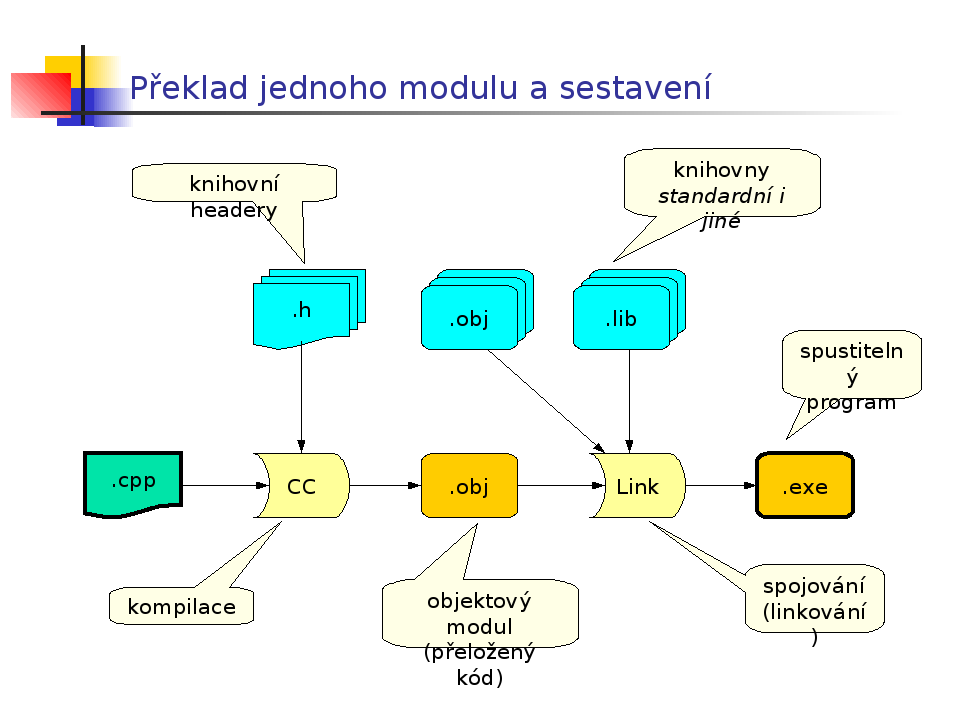
\includegraphics[width=10cm]{informatika/programovanie/obrazky/oddelenypreklad01.png}
\end{center}
\par\begin{center}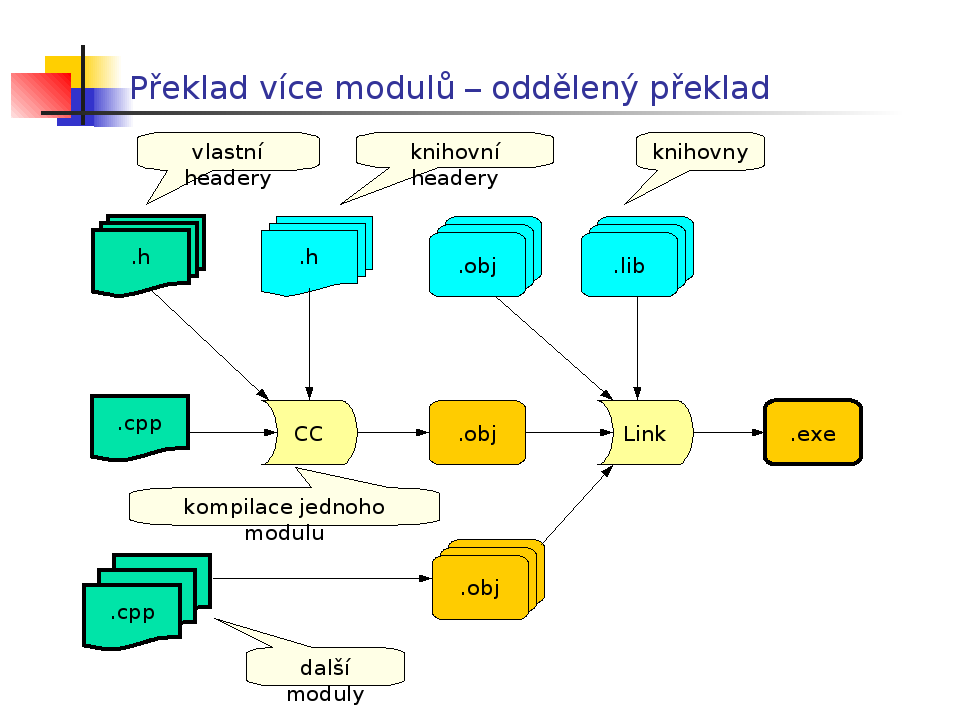
\includegraphics[width=10cm]{informatika/programovanie/obrazky/oddelenypreklad02.png}\end{center}
Smysl odděleného překladu modulů je urychlení celkového překladu -- nepřekládat to, co se od minula nezměnilo. Oddělený překlad dnes díky automatizaci makefily (viz níže) a integrovanými prostředími není téměř pro programátora vidět.

...pri tomto slide je vhodné ujasniť si, ako funguje statické a dynamické linkovanie (ako, kde a kedy sa opravujú adresy objektov atď.):
\begin{pitemize}
    \item \emph{Statické linkování} \\ Po odděleném překladu jednotlivé object moduly ještě neobsahují přímo adresy všech funkcí a externích identifikátorů, jen odkazy na ně. Linker se postará o jejich spojení dohromady. Je nutné, aby jména byla unikátní, takže u přetížených a virtuálních funkcí, jako je v C++, musí bý jména zpotvořena tak, aby ukazovala i třídu, namespace, parametry a jejich typy. To má na starosti compiler a říká se tomu \emph{name mangling}.
    \item \emph{Dynamické linkování} \\ Nastává po volání operačního systému -- zavedení dynamické knihovny do paměti. Jsou dvě možnosti jeho provedení, první je právě při zavádění knihovny, kdy se odkazy na všechny funkce (a mezi nimi navzájem) naplní správnými hodnotami (podle bázové adresy, na kterou se knihovna do paměti nahraje). Druhá možnost je použití dvou pointerů při volání funkcí z knihovny -- to se vytvoří tabulka skutečných adres, na kterou se z knihovny ukazuje. První možnost trvá déle při zavádění knihovny, druhá je zase pomalejší při provádění, ale umožňuje kód knihovny beze změn sdílet více procesy.
\end{pitemize}


\par\begin{center}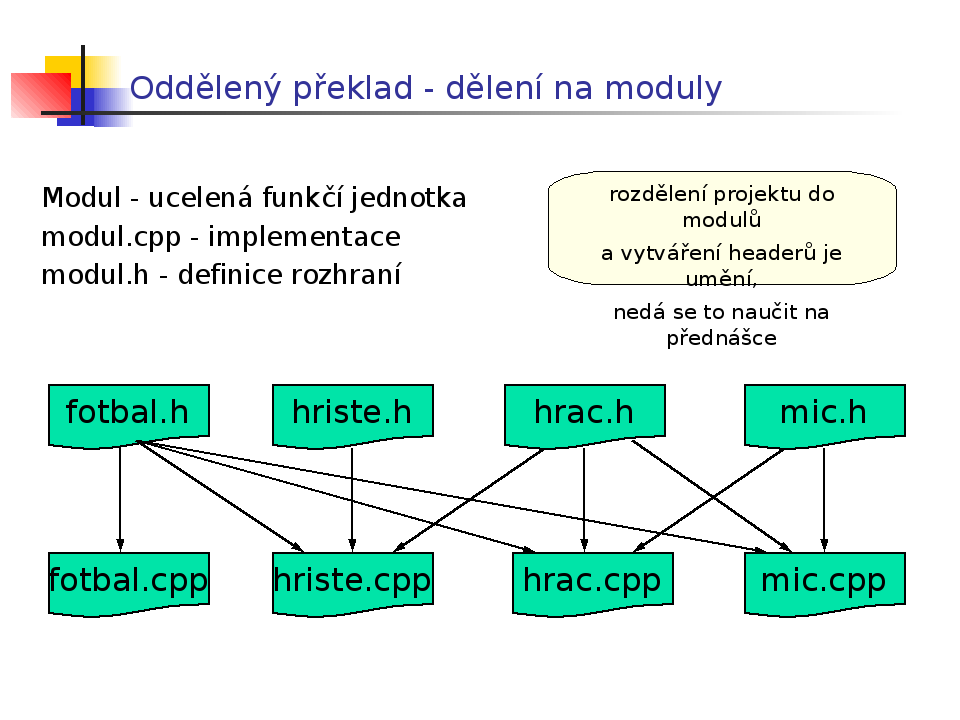
\includegraphics[width=10cm]{informatika/programovanie/obrazky/oddelenypreklad03.png}\end{center}

\emph{Linker} je program, který prijímá jeden alebo více objektů generovaných kompilátorem a složí je v jeden spustitelný program.

Objektový kód, nebo objektový soubor je reprezentace kódu, který kompilátor nebo assembler vytvoří zpracováním zdrojového kódu. Objektové soubory obsahují kompaktní kód, často nazývaný \uv{binárky} :-) Linker se typicky používá na vytvoření spustitelnýho souboru nebo knihovny spojením (slinkováním) objektových souborů. Základní častí objektového souboru je strojový kód (kód přimo vykonávaný CPU počítače).

\subsubsection*{Makefile}

Smyslem programu \emph{make} je řízení překladu a linkování. Popis závislostí jednotlivých modulů a hlavičkových na sobě je definován v 1 textovém souboru -- \emph{Makefile} (tj. které soubory je nutné mít aktuální/vytvořené pro překlad kterého souboru). Make vždy po změně souboru přeloží jen to, co na něm závisí.
Formát souboru make:
\begin{verbatim}
targets: files; 
        commands; #comment; line-begin\
        line contd.;
\end{verbatim}
Targets -- cíle činností / cílové soubory, možno definovat vic, při spuštění make bez parametrů se bere první; univ. nástroj (nejen pro překlad C/C++). Lze definovat i vlastní makra (příkazem \texttt{<název makra> = <string>}) a pak je používat (\texttt{\$\{makro\}}).

\subsection{Neprocedurální programování, logické programování}

\subsubsection*{Neprocedurální programování}
\emph{Deklarativní programování} je postaveno na paradigmatu, podle něhož je program založen na tom, co se počítá a ne jak se to počítá. Je zde deklarován vstup a výstup a celý program je chápán jako funkce vyhodnocující vstupy podávající jediný výstup. Například i webovské stránky jsou deklarativní protože popisují, jak by stránka měla vypadat -- titulek, font, text a obrázky -- ale nepopisují, jak konkrétně zobrazit stránky na obrazovce.

\emph{Logické programování} a \emph{funkcionální programování} jsou poddruhy deklarativního programování. Logické programování využívá programování založené na vyhodnocování vzorů - tvrzení a cílů. Klasickým zástupcem jazyka pro podporu tohoto stylu je Prolog.

Tento přístup patří pod deklarativní programování stejně jako funkcionální programování, neboť deklaruje, co je vstupem a co výstupem, a nezabývá se jak výpočet probíhá. Naopak program jako posloupnost příkazů je paradigma imperativní.

\emph{Funkcionální programování} patří mezi deklarativní programovací principy.

Alonzo Church vytvořil formální výpočtový model nazvaný $\lambda$-kalkul. Tento model slouží jako základ pro funkcionální jazyky. Funkcionální jazyky dělíme na:
\begin{pitemize}
	\item typované - Haskell
	\item netypované - Lisp, Scheme
\end{pitemize}

Výpočtem funkcionálního programu je posloupnost vzájemně ekvivalentních výrazů, které se postupně zjednodušují. Výsledkem výpočtu je výraz v normální formě, tedy dále nezjednodušitelný. Program je chápán jako jedna funkce obsahující vstupní parametry mající jediný výstup. Tato funkce pak může být dále rozložitelná na podfunkce.

\subsubsection*{Prolog}

Prolog je logický programovací jazyk. Název Prolog pochází z francouzského programmation en logique (\uv{logické programování}). Byl vytvořen Alainem Colmerauerem v roce 1972 jako pokus vytvořit programovací jazyk, který by umožňoval vyjadřování v logice místo psaní počítačových instrukcí. Prolog patří mezi tzv. deklarativní programovací jazyky, ve kterých programátor popisuje pouze cíl výpočtu, přičemž přesný postup, jakým se k výsledku program dostane, je ponechán na libovůli systému.

Prolog je využíván především v oboru umělé inteligence a v počítačové lingvistice (obzvláště zpracování přirozeného jazyka, pro nějž byl původně navržen). Syntaxe jazyka je velice jednoduchá a snadno použitelná pravě proto, že byl původně určen pro počítačově nepříliš gramotné lingvisty.

Prolog je založen na \emph{predikátové logice prvního řádu} (konkrétně se omezuje na Hornovy klauzule). Běh programu je pak představován aplikací dokazovacích technik na zadané klauzule. Základními využívanými přístupy jsou \emph{unifikace}, \emph{rekurze} a \emph{backtracking}.

Interpret Prologu se snaží nalézt nejobecnější substituci, která splní daný cíl - tzn. nesubstituuje zbytečně, pokud nemusí (použití interních proměnných -- \_123 atd.). Za dvě proměnné může být substituována jedna interní proměnná (např. při hledání svislé úsečky -- konstantní X souřadnice) -- tomu se říká \emph{unifikace} proměnných. Pro proměnnou, jejíž hodnota může být libovolná, se v prologu užívá znak \uv{\_}. 

Datové typy v prologu se nazývají \emph{termy}. Základním datovým typem jsou \emph{atomy} (začínají malým písmenem, nebo se skládají ze speciálních znaků (\texttt{+ - * / \dots}, nebo jsou to znakové řetězce (\texttt{'text'})). Dále \uv{jsou} v prologu čísla (v komerčních implementacích i reálná), proměnné (velké písmeno) a struktury (definované rekursivně - pomocí funktoru dané arity a příslušným počtem termů, které jsou jeho argumenty -- \texttt{okamzik(datum(1,1,1999),cas(10,10))}). Posledním typem proměnných jsou seznamy, které jsou probírány později.

\medskip\textbf{Základní principy}:

Programování v Prologu se výrazně liší od programování v běžných procedurálních jazycích jako např. C. Program v prologu je databáze faktů a pravidel (dohromady se faktům a pravidlům paradoxně říká procedury), nad kterými je možno klást dotazy formou tvrzení, u kterých Prolog zhodnocuje jejich pravdivost (dokazatelnost z údajů obsažených v databázi).

Například lze do databáze uložit fakt, že Monika je dívka:
\begin{verbatim}
dívka(monika).
\end{verbatim}

Poté lze dokazatelnost tohoto faktu prověřit otázkou, na kterou Prolog odpoví yes (ano):
\begin{verbatim}
?- dívka(monika).
     yes.
\end{verbatim}

Také se lze zeptat na všechny objekty, o kterých je známo, že jsou dívky (středníkem požadujeme další výsledky):
\begin{verbatim}
?- dívka(X).
     X = monika;
     no.
\end{verbatim}

Pravidla (závislosti) se zapisují pomocí implikací, např.
\begin{verbatim}
syn(A,B) :- rodič(B,A), muž(A).
\end{verbatim}

Tedy: pokud B je rodičem A a zároveň je A muž, pak A je synem B. První části pravidla (tj. důsledku) se říká hlava a všemu co následuje za symbolem \texttt{:-} (tedy podmínkám, nutným pro splnění hlavy) se říká tělo. Podmínky ke splnění mohou být odděleny buď čárkou (pak jde o konjunkci, musejí být splněny všechny), nebo středníkem (disjunkce), přičemž čárky mají větší prioritu.

\medskip\textbf{Příklad}:

Typickou ukázkou základů programování v Prologu jsou rodinné vztahy.
\begin{verbatim}
sourozenec(X,Y) :- rodič(Z,X), rodič(Z,Y).
rodič(X,Y) :- otec(X,Y).
rodič(X,Y) :- matka(X,Y).
muž(X) :- otec(X,_).
žena(X) :- matka(X,_).
matka(marie,monika).
otec(jiří,monika).
otec(jiří,marek).
otec(michal,tomáš).
\end{verbatim}

Prázdný seznam je označen atomem $[]$, neprázdný se tvoří pomocí funktoru \texttt{'.'} (tečka) - \texttt{.(Hlava,Tělo)}. V praxi se to (naštěstí ;-)) takhle složitě rekurzivně zapisovat nemusí, stačí napsat \texttt{[a,b,c...]}, resp \texttt{[Začátek | Tělo]}, kde začátek je výčet prvků (ne seznam) stojících na začátku definovaného seznamu, a tělo je (rekurzivně) seznam (např. \texttt{[a,b,c|[]]}).

Aritmetické výrazy se samy o sobě nevyhodnocují, dokud jim to někdo nepřikáže. Takže např. predikát \texttt{5*1 = 5} by selhal. Vyhodnocení se vynucuje pomocí operátoru \emph{is} (pomocí = by došlo jen k unifikaci) - není to ale ekvivalent \uv{\texttt{=}} z jiných jazyků. Tento operátor se musí použít na nějakou volnou proměnnou a aritmetický výraz, s jehož hodnotou bude tato proměnná dále svázaná (jako např. \texttt{X is 5*1,X=5} uspěje).

Důležitý je i \emph{operátor řezu} (značíme vykřičníkem). Tento predikát okamžitě uspěje, ale při tom zakáže backtrackování přes sebe zpět. (\texttt{prvek1(X,[X|L]):-!. prvek1(X,[\_|L]):-prvek1(X,L).} - je-li prvek nalezen, je zakázán návrat = najde jen první výskyt prvku). Dále je důležitá negace (\texttt{not(P):- P, !, fail. not(P).} -- uspěje, pokud se nepodaří cíl P splnit). Řez tedy umožňuje ovlivňovat efektivitu prologovských programů, definovat vzájemně se vylučující použití jednotlivých klauzulí procedury, definovat negaci atd.

\subsubsection*{Haskell}
Haskell je standardizovaný funkcionální programovací jazyk používající zkrácené vyhodnocování, pojmenovaný na počest logika Haskella Curryho. Byl vytvořen v 80. letech 20. století. Posledním polooficiálním standardem je Haskell 98, který definuje minimální a přenositelnou verzi jazyka využitelnou k výuce nebo jako základ dalších rozšíření. Jazyk se rychle vyvíjí, především díky svým implementacím Hugs a GHC (viz níže).

Haskell je jazyk dodržující \emph{referenční transparentnost}. To, zjednodušeně řečeno, znamená, že tentýž (pod)výraz má na jakémkoliv místě v programu stejnou hodnotu. Mezi další výhody tohoto jazyka patří přísné \emph{typování proměnných}, které programátorovi může usnadnit odhalování chyb v programu. Haskell plně podporuje práci se soubory i standardními vstupy a výstupy, která je ale poměrně složitá kvůli zachování referenční transparentnosti. Jako takový se Haskell hodí hlavně pro algoritmicky náročné úlohy minimalizující interakci s uživatelem.

\medskip\textbf{Příklady}:

Definice funkce faktoriálu:
\begin{verbatim}
fac 0 = 1
fac n = n * fac (n - 1)
\end{verbatim}

Jiná definice faktoriálu (používá funkci product ze standardní knihovny Haskellu):
\begin{verbatim}
fac n = product [1..n]
\end{verbatim}

Naivní implementace funkce vracející n-tý prvek Fibonacciho posloupnosti:
\begin{verbatim}
fib 0 = 0 
fib 1 = 1 
fib n = fib (n - 2) + fib (n - 1)
\end{verbatim}

Elegantní zápis řadícího algoritmu quicksort:
\begin{verbatim}
qsort [] = []
qsort (pivot:tail) = 
  qsort left ++ [pivot] ++ qsort right
  where
    left = [y | y <- tail, y < pivot]
    right = [y | y <- tail, y >= pivot]
\end{verbatim}

TODO: popsat stráže (případy, otherwise), seznamy, řetězení, pattern matching u parametrů funkcí, lok. definice (where, let) -- patří to sem?

\subsubsection*{Lisp}

Lisp je funkcionální programovací jazyk s dlouhou historií. Jeho název je zkratka pro List processing (zpracování seznamů). Dnes se stále používá v oboru umělé inteligence. Nic ale nebrání ho použít i pro jiné účely. Používá ho například textový editor Emacs, GIMP či konstrukční program AutoCAD.

Další jazyky od něj odvozené jsou například Tcl, Smalltalk nebo Scheme.


\medskip\textbf{Syntaxe}:
Nejzákladnějším zápisem v Lispu je seznam. Zapisujeme ho jako:
\begin{verbatim}
(1 2 "ahoj" 13.2)
\end{verbatim}

Tento seznam obsahuje čtyři prvky:
\begin{pitemize}
	\item celé číslo 1
	\item celé číslo 2
	\item text \uv{ahoj}
	\item reálné číslo 13,2
\end{pitemize}

Jde tedy o uspořádanou čtveřici. Všimněte si, že závorky nefungují tak jako v matematice, ale pouze označují začátek a konec seznamu. Seznamy jsou v Lispu implementovány jako binární strom degenerovaný na jednosměrně vázaný seznam. Co se seznamem Lisp udělá, záleží na okolnostech.

\textbf{Příkazy}: Příkazy píšeme také jako seznam, první prvek seznamu je však název příkazu. Například sčítání provádíme příkazem +, což interpreteru zadáme takto:
\begin{verbatim}
(+ 1 2 3)
\end{verbatim}
Interpretr odpoví 6.

\textbf{Ukázka kódu}:
Program hello world lze zapsat několika způsoby. Nejjednoduší vypadá takto:
\begin{verbatim}
(format t "Hello, World!")
\end{verbatim}

Funkce se v Lispu definují pomocí klíčového slova defun:
\begin{verbatim}
(defun hello ()
        (format t "Hello, World!")
)
(hello)
\end{verbatim}

Na prvních dvou řádcích je definice funkce hello, na třetím řádku je tato funkce svým jménem zavolána.
Funkcím lze předávat i argumenty. V následujícím příkladu je ukázka funkce fact, která vypočítá faktoriál zadaného čísla:
\begin{verbatim}
(defun fact (n)
        (if (= n 0)
                1
                (* n (fact (- n 1)))
        )
)
\end{verbatim}
Pro výpočet faktoriálu čísla 6 předáme tuto hodnotu jako argument funkci fact:
\begin{verbatim}
(fact 6)
\end{verbatim}
Návratovou hodnotou funkce bude hodnota 720.

\subsubsection*{Logické programování}
TODO (není součástí otázek pro obor Programování)

\subsection{Struktura překladače, lexikální, syntaktická analýza}

Zdroj: poznámky a slidy z přednášek Principy překladačů Dr. J. Yaghoba

\subsubsection*{Překladače}

\begin{definiceN}{Překladač}
Formální definice: \emph{překladač} je zobrazení $L_{in}\to L_{out}$ pro nějaké dva jazyky $L_{in},L_{out}$, vstupní generovaný gramatikou $G_{in}$, výstupní generovaný gramatikou $G_{out}$ nebo přijímaný automatem $A_{out}$. Je to takové zobrazení, kde $\forall w\in L_{in}\ \exists w'\in L_{out}$. Pro $w\notin L_{in}$ zobrazení neexistuje.

Neformálně jde o stroj, který nějaký zdrojový kód (v nějakém zdrojovém jazyce) převádí na cílový kód (v cílovém jazyce) a případně vypisuje chybová hlášení.

Definice neříká nic o třídách jazyků a gramatik, ve kterých překladač operuje. Běžné programovací jazyky jsou \uv{plus minus} bezkontextové -- nebo se na bezkontextové převádějí, aby byly rozpoznatelné něčím prakticky implementovatelným (tedy zásobníkovým automatem, Turingovy stroje jsou poněkud složité).
\end{definiceN}


\begin{priklady}
Příklady použití překladačů:
\begin{pitemize}
    \item (překvapivě) překlad programů, psaných v nějakém vyšším programovacím jazyce, do strojového kódu cílové platformy
    \item syntax-highlighting (většinou lexikálně řízený)
    \item pretty printer
    \item statické kontroly programu (hledání chyb bez spouštění programů)
    \item interpretery (např. skriptovacích jazyků, run-time moduly pro interpretované jazyky jako je Java)
    \item databázové stroje, dotazovací jazyky
\end{pitemize}
\end{priklady}


\begin{obecne}{Překlad programu}
Program (pro jednoduchost jediný modul) se 
\begin{penumerate}
    \item ze zdrojového kódu v nějakém programovacím jazyce \emph{preprocesorem} (což je taky překladač, upravující zdrojový kód na textové úrovni) převede na textový soubor (připravený pro další překlad),
    \item \emph{překladačem} se převede dál do assemblerového kódu (jde o kód v jiném jazyce, mnohem bližším cílové architektuře -- jde o textový popis instrukcí procesoru),
    \item \emph{assemblerem} se převádí na \uv{object-file} -- modul, ve kterém už jazyk odpovídá strojovému kódu cílové CPU,
    \item nakonec \emph{linker}, resp. \emph{loader} připojí další informace a vytvoří finální spustitelný kód.
\end{penumerate}
\end{obecne}

\begin{obecne}{Fáze překladu překladačem}
Tradičně se překladače dělí na dvě fáze -- \emph{front-end} a \emph{back-end}. První z nich je zaměřená hlavně na analýzu zdrojového kódu po lexikální a syntaktické stránce a její převod do nějakého mezikódu, tj. přípravu pro back-end. Úkolem back-endu je pak z předpřipravené formy vygenerovat finální kód v cílovém jazyce.

První fáze se dále dělí na tyto části:
\begin{penumerate}
    \item \emph{lexikální analýza} -- převádí vstupní text do binární formy, na sled identifikátorů a konstant; hodnoty objektů ukládá do spec. tabulek 
    \item \emph{syntaktická analýza} -- abstraktní část, nezajímá se o hodnoty a význam elementů jazyka, úkolem je rozpoznat, zda vstupní slovo (vstup) patří do jazyka; v dnešních překladačích staví tzv. \uv{syntaktický strom} kódu
    \item \emph{sémantická analýza} -- zkoumá sémantiku (význam, smysl) elementů jazyka (např. u sčítání proměnných kontrola typů, používání definovaných proměnných atd.)
    \item \emph{generování mezikódu} -- úzce svázané se sémantickou analýzou, načítá hodnoty lexikálních elementů z tabulek a vytváří binární formu kódu, v ideálním případě nezávislou na vstupním ani výstupním jazyce
    \item \emph{optimalizace nad mezikódem} -- díky překladu do nějakého abstraktního mezikódu lze nad ním potom provádět různé obecné (teoreticky dokázané) optimalizace, aby byl výsledný kód ekvivalentní s původním, ale rychlejší při provádění cílovým strojem
\end{penumerate}

Backend má na starosti hlavně
\begin{penumerate}
    \item \emph{generování kódu} -- vytváří už kód pro konkrétní cílový stroj / architekturu / CPU. 
    \item \emph{optimalizace nízkoúrovňového kódu} -- optimalizace, zaměřené na vlastnosti konkrétních CPU a cílový jazyk (tj. takové, které nad obecným mezikódem s vysokou abstrakcí provést nejde)
\end{penumerate}

Všechny fáze překladače (většinou, když se pominou třeba staší verze GCC a podobně) sdílejí jednotné \emph{tabulky symbolů} -- hodnot lexikálních elementů a jiných věcí a obsluhu chyb. Překladač musí rozpoznat všechny chyby, ale bez velké časové režie, navíc nesmí mít falešné poplachy. Taky by neměl vyrábět chyby sám ;-).

V dřívějších překladačích se vstupní kód procházel několikrát, protože nebylo technicky možné ho udržet celý v paměti. Dnes je potřeba většinou jen jeden přechod, ale někdy je nutných víc (např. dopředné skoky v assembleru -- nevím ještě jak daleko skáču).
\end{obecne}

\begin{poznamkaN}{Syntax-driven compilation}
Nejdůležitější částí dnešních překladačů bývá syntaktická analýza; provádí se často najednou se sémantickou analýzou a generováním mezikódu -- vše mívá na starosti jediný zásobníkový automat. Navíc si často sám vyvolává lexikální analýzu, ta je jím tedy řízená, takže se taková technika označuje \emph{syntaxí řízený překlad}.
\end{poznamkaN}

\begin{obecne}{Automatické generování (částí) překladače}
Protože dnešní programovací jazyky jsou relativně složité (gramatiky které je generují mají řádově stovky přepisovacích pravidel), konstrukce automatů přijímajících takové jazyky \uv{ručně} je příliš náročná. Proto existují nástroje, které generují některé části překladače -- generátor lexikálních analyzátorů -- \uv{scannerů} -- (popíšu lexikální elementy a struktury a co s nimi dělá a vypadne mi analyzátor jako kód v jazyce C) je např. \emph{Flex}, pro výrobu parserů (syntaktických analyzátorů) z popisu gramatiky slouží např. \emph{Bison}, \emph{Coco/R} nebo \emph{ANTLR}. Některé známé překladače mají ale i tak ručně generované parsery (GCC).

Existují i generátory generátorů kódu (ale jejich méně, protože to je dost složité) -- pro popis výstupního CPU dostanu z instrukčního mezikódu kód přímo pro něj. Instrukční mezikód může být pro více architektur úplně stejný. Příkladem tohoto je \emph{Mono JIT Compiler}.
\end{obecne}


\begin{obecne}{Mezikód}
(Vysokoúrovňový) \emph{mezikód} je vlastně jakési rozhraní pro přechod (rozdělení i spolupráci) mezi front-endem a back-endem. Jde o binární reprezentaci zdrojového kódu, má být nezávislý na vstupním i výstupním jazyce. Pokud tomu tak je, je možné např. kombinovat různé back-endy a front-endy, jako tomu je u GCC (více back-endů pro 1 front-end) nebo .NET (více front-endů). Většinou ale je mezikód o něco posunutý buď více k závislosti na back-endu nebo na front-endu.

Mezikód je možné reprezentovat několika způsoby -- např. syntaktickým stromem (vhodné v paměti), postfixovým zápisem (linearizace stromu) nebo tříadresovým kódem (lineární, sekvence příkazů $x:= y\ \mathrm{op}\ z$).
\end{obecne}

\begin{obecne}{Graf toku řízení}
Graf toku řízení je graf, vytvářený překladači (větš. pro 1 funkci) za účelem optimalizací a také generování výsledného kódu. Uzly -- \emph{základní bloky} -- jsou nepřerušované výpočty (bez instrukcí skoků a bez cílů skoků uvnitř bloků), z nichž první instrukce bývá cílem skoku nebo vstupním bodem funkce. Hrany pak reprezentují skoky -- pro podmíněné skoky a case příkazy pak z uzlů vede více hran.
\end{obecne}

\subsubsection*{Lexikální analýza}

\begin{definiceN}{Lexikální analýza}
Lexikální analýza je část překladače, zodpovědná za rozpoznávání jednotlivých nedělitelných elementů zdrojového jazyka (např. klíčová slova, identifikátory, závorky atd.) a jejich převod na nějakou binární reprezentaci, vhodnou pro syntaktickou analýzu (např. uložení názvů identifikátorů do tabulek symbolů). V zásadě jde o rozpoznávání regulárních výrazů. Historicky šlo o provedení analýzy na celém zdrojáku a přeposlání do další fáze, dnes je většinou ovládaná ze syntaktické analýzy (opakované volání \uv{vrať další element}). Slouží také ke zvětšení \uv{výhledu} dalších fází (jedním elementem přestává být jeden znak, je jím jeden element vstupního jazyka).
\end{definiceN}

\begin{definiceN}{Token, pattern}
\emph{Token} je výstup lexikální analýzy -- jeden nedělitelný element zdrojového jazyka. Je zároveň vstupem syntaktické analýzy (tam se nazývá \emph{terminál}). Lexikální analýza uvažuje množinu řetězců, které produkují pro syntaktickou analýzu stejný token (např. díky ignore-caseovosti nebo jako důsledek sloučení všech řetězcových nebo číselných konstant pod stejný token, protože s nimi je dále nakládáno bez ohledu na hodnotu). Množina řetězců, produkujících daný token, se popisuje urč. pravidly -- \emph{patternem}, kde se obvykle užívá regulárních výrazů.
\end{definiceN}

\begin{definiceN}{Lexém}
\emph{Lexém} neboli \emph{lexikální element} je sekvence znaků ve zdrojovém kódu, která (většinou) odpovídá nějakému patternu nějakého tokenu. Např. komentáře ale jako svůj výstup žádný token nemají.
\end{definiceN}

\begin{definiceN}{Literál}
\emph{Literál} je konstanta ve vstupním jazyce -- má svoji hodnotu (atribut), ukládanou do tabulek symbolů.
\end{definiceN}

\begin{poznamkaN}{Atributy tokenů}
Je-li jeden token rozpoznáván více patterny, nebo je-li to literál, má nějaké další atributy (většinou jenom jeden), které jeho význam upřesňují -- např. token \uv{relační operátor} má zpřesnění \uv{menší nebo rovno}, token \uv{číselný literál} má zpřesnění \uv{12345}.
\end{poznamkaN}

\begin{obecne}{Problémy lex. analýzy}
Mezi některé problémy, které syntaktická analýza musí řešit, patří
\begin{pitemize}
    \item Počítání zarovnání -- některé jazyky (Python) mají zarovnání na řádce jako svoji syntaktickou konstrukci
    \item Identifikátory s mezerami (rozlišit identifikátor od jiné konstrukce, i víceslovné)
    \item Klíčová slova jako identifikátory (někdy se mohou překrývat)
    \item Kontextově závislé tokeny -- token závisí na jiných informacích (např. \texttt{a*b;} v C -- jde o násobení, nebo deklaraci pointerové proměnné), tady je nutné tokeny slučovat pro oba významy ???
\end{pitemize}
\end{obecne}

\begin{obecne}{Pozadí lex. analýzy}
Na pozadí lexikálního analyzátoru většinou pracuje nějaký konečný automat (protože rozpoznávání regulárních výrazů -- hodnotou reg. výrazu je reg. jazyk -- je práce pro konečné automaty). Po každém rozpoznaném tokenu je potřeba automat uvést zpět do výchozího stavu.
\end{obecne}

\begin{obecne}{Lexikální chyby}
Chyba v lexikální analýze nastane tehdy, když konečný automat nemůže pokračovat dál a není v koncovém stavu (např. pokud nalezne neplatný znak, nebo neukončený řetězec na konci řádky apod.). Většina lexikálních analyzátorů (pomineme Turbo Pascal ;-)) by měla být schopna nějakého \uv{rozumného} zotavení z chyby -- vypsat chybu a domyslet chybějící znak nebo neplatný znak ignorovat apod., tj. nezastavit se na první chybě. I logické zotavení může ale scanner úplně rozhodit a ten pak vyhazuje nesmyslné chyby. Je také spousta chyb, které lexikální analýza nepozná a projeví se až u syntaktické analýzy, např. \texttt{beign} místo \texttt{begin}, chápané jako identifikátor. 
\end{obecne}

\begin{poznamkaN}{Bufferování vstupu}
Syntaktická analýza časově zabere cca 60-80\% překladu, takže se pro její urychlení používá bufferování -- nečte se po znacích, ale o něco napřed. Problémem pak jsou např. \texttt{\#include} direktivy (jsou-li ve vstupním jazyce) -- v okamžiku vložení jiného souboru je scanner v nějakém stavu apod.; scannery musí mít pak možnost přepínat mezi více vstupními soubory (manipulovat s několika buffery).
\end{poznamkaN}

\subsubsection*{Syntaktická analýza}

\begin{definiceN}{Syntaktická analýza}
Syntaktická analýza je část překladače, zodpovědná za:
\begin{penumerate}
    \item rozhodnutí, zda dané slovo (vstup) patří do zpracovávaného jazyka
    \item syntaxí řízený překlad
    \item stavbu derivačního stromu (nalezení přepisovacích pravidel ze startovacího neterminálu gramatiky na vstupní posloupnost tokenů -- terminálů)
\end{penumerate}

Většina programovacích jazyků je bezkontextová, proto je syntaktická analýza představována zásobníkovým automatem. Syntaktická analýza operuje s gramatikou daného jazyka (snaží se o přepis abstraktních neterminálů na terminály -- tokeny jazyka).
\end{definiceN}

\begin{definiceN}{Derivační strom}
Derivační strom je \uv{grafická} reprezentace slova vstupního jazyka, nebo spíše derivací, které bylo potřeba provést, aby se v gramatice startovací symbol přepsal na dané slovo (posloupnost terminálů). Uzly takového grafu jsou neterminály i terminály gramatiky jazyka (v listech ale jsou jen terminály, ve vnitřních uzlech neterminály). Hrany grafu představují přepsání podle pravidla gramatiky -- vedou od neterminálu který se přepisuje, ke všem neterminálům nebo terminálům na které se přepisuje (mluvíme o bezkontextových gramatikách, takže na levé straně stojí jen jeden neterminál).

Přepsání v gramatice bohužel nemusí být jednoznačné (tj. pro stejnou posloupnost neterminálů existuje více platných derivačních stromů). Přikladem je problém \uv{dangling else} z jazyků typu Pascal nebo C -- mám-li za sebou 2x \texttt{if-then} a pak jedno \texttt{else}, nemusí být (z gramatiky) jasné, ke kterému \texttt{if-then} ono \texttt{else} patří. Takové problémy lze (a je nutné) odstranit převodem na jednoznačnou gramatiku (např. přes další neterminál).
\end{definiceN}

\begin{obecne}{Levá rekurze, levá faktorizace, nebezkontextovost}
Levá rekurze v gramatice se objevuje, pokud je v ní neterminál $A$, pro který platí $A\Rightarrow^{*} A\alpha$ pro nějaké $\alpha\neq\lambda$. Tj. přes $A$ je možné projít kolikrát chci a vytvořit posloupnost $\alpha\alpha\dots$. Pokud parser začíná u startovacího neterminálu a hledá derivace na na terminály \uv{shora dolů} (to jeden z druhů scannerů dělá), neví jakou hloubku rekurze má použít. Proto je nutné i levou rekurzi, stejně jako nejednoznačnosti, z gramatiky napřed odstranit její úpravou (zde opět pomůže přechod přes nový neterminál).

Problémem je i levá faktorizace -- případ, kdy se v gramatice vyskytují pravidla jako $A\to \alpha\beta$ a zároveň $A\to \alpha\gamma$. I ten je možné řešit úpravou gramatiky (přenos rozhodnutí na pozdější dobu, kdy bude známo, který ze symbolů $\beta,\gamma$ si vybrat).

Může se také i pro běžné konstrukce z programovacích jazyků stát, že nevyhovují bezkontextovým gramatikám -- např. kontrola deklarace identifikátoru před použitím, kontrola počtu parametrů funkce apod. Zde syntaktická analýza bezkontextovým způsobem nestačí a tyto případy je třeba řešit jinak.
\end{obecne}

\begin{definiceN}{Názvosloví gramatik, FIRST a FOLLOW}
Gramatiky se v teorii překladačů označují dvěma až třemi znaky a číslem v závorce, obecně ve tvaru $PXY(k)$, kde:
\begin{pitemize}
    \item $X$ je směr čtení vstupu (V našem případě vždy $L$, tj. zleva doprava),
    \item $Y$ jsou druhy derivace ($L$ – levé, $R$ – pravé derivace),
    \item $P$ označuje prefix (ještě jemnější dělení na třídy u některých gramatik) a
    \item $k$ představuje \emph{výhled} (lookahead), každý parser totiž vidí jen na jeden nebo několik tokenů dopředu a další neuvažuje. Obvykle je to celé číslo, většinou 1, ale také 0 nebo obecně $k$.
\end{pitemize}
Příklady: $LL(1), LR(0), LR(1), LL(k), SLR(1), LALR(1)$

Množiny \emph{FIRST} a \emph{FOLLOW} představují množinu použitelných neterminálů na urč. místech (začátky řetězců derivovaných z nějakého pravidla, resp. řetězce které mohou následovat po nějakém neterminálu) a používají se pro konstrukci parserových automatů pro nějakou gramatiku.
\end{definiceN}

TODO: formalizovat FIRST a FOLLOW, neni to moc slozite?

\begin{definiceN}{Analýza shora dolů}
Analýza shora dolů je technika parserů, kdy se parser snaží najít nejlevější derivaci pro vstupní řetězec. Pokouší se tedy zkonstruovat derivační strom pro daný vstup počínaje kořenem a přidáváním uzlů do stromu -- rozhoduje se, podle kterého pravidla gramatiky přepíše. Pravidlo pro odstranění nejednoznačnosti je provádění \emph{jen levých derivací}, proto pak automatům vadí levá rekurze a musí se odstraňovat. Techniky pro nalezení přepisovacího pravidla jsou:
\begin{pitemize}
    \item \emph{Rekurzivní sestup} pomocí procedur -- pro každý neterminál existuje jedna procedura, která se rozhodne, které pravidlo použije na základě výhledu. Pro rozhodování se sestavují množiny FIRST a FOLLOW každého neterminálu. Potom musí zkontrolovat, jestli pravá strana tohoto pravidla odpovídá vstupu (přičemž výskyt neterminálu na pravé straně znamená zavolání jemu příslušné procedury).     
    \item \emph{Nerekurzivní analýza s predikcí} -- je implementováno automatem s explicitním zásobníkem: ten má \emph{parsovací tabulku}, která se liší podle gramatiky (sama práce automatu je vždy stejná) -- jsou v ní řádky odpovídající neterminálům a sloupce terminálům, v políčkách jsou přepisovací pravidla  nebo chyby. Na zásobník automatu se ukládají symboly gramatiky a ze vstupu se čtou (lineárně terminály). V každém kroku se automat rozhodne podle vstupu a vrcholu zásobníku -- je-li tam terminál, vyhodí se a ukazatel vstupu se posune (nebo se skončí); je-li na zásobníku neterminál, rozhoduje se podle tabulky (položka určená vstupem a neterminálem, buďto se použije přepisovací pravidlo nebo skončí chybou). Konstrukce tabulky je opět závislá na množinách FIRST a FOLLOW.
\end{pitemize}
Analýza shora dolů je používána v parserech jednoduchých jazyků ($LL(1)$ gramatiky s řešením konfliktů zvětšením výhledu na $k$ terminálů) -- v generátorech parserů ANTLR a Coco/R, například.
\end{definiceN}

\begin{definiceN}{Analýza zdola nahoru, LR automat}
Parsery s analýzou zdola nahoru se pokoušejí najít pozpátku nejpravější derivaci pro vstupní řetězec -- zkonstruovat derivační strom pro daný vstup počínaje listy a stavěním zespodu až po kořen stromu. V jednom redukčním kroku je tak podřetězec odpovídající pravé straně pravidla gramatiky nahrazen neterminálem z levé strany pravidla. Analýza zdola nahoru se používá ve např. v generátoru parserů Bison -– je schopná vytvořit parsery pro $LALR(1), GLR(1)$ gramatiky, které jsou oproti $LL(1)$ parserům \uv{silnější} (Třída rozpoznávaných jazyků LR(1) je vlastní nadmnožina LL(1)), všechny běžné programovací jazyky zapsatelné bezkontextovou gramatikou sem patří. Navíc se dá implementovat zhruba stejně efektivně jako metoda shora dolů.

V analýze zdola nahoru se používá nějaký zásobníkový automat (\emph{LR automat}) čtoucí ze vstupu, parametrizovaný tabulkami \emph{ACTION} a \emph{GOTO}. Na zásobníku se pak uchovávají stavy a symboly gramatiky (nebo jen stavy). Vrchol zásobníku představuje aktuální stav. V počáteční konfiguraci je pointer vstupu nastavený na začátek a na zásobníku je počáteční stav. V každém kroku podle stavu a tokenu na vstupu adresuji tabulku ACTION a získám akci k provedení:
\begin{pitemize}
    \item \emph{SHIFT} $s$ -- posune vstup o 1 terminál, který přidá na zásobník spolu s novým stavem $s$.
    \item \emph{REDUCE} $A\to\alpha$ -- zruší ze zásobníku tolik dvojic stavů a symbolů, jak dlouhé je $\alpha$, na zásobník dá $A$ a stav, který najde v tabulce GOTO na pozici odpovídající neterminálu $A$ a aktuálnímu stavu
    \item \emph{ACCEPT} -- generuje nějaký výstup, slovo je úspěšně rozpoznáno
    \item \emph{ERROR} -- zahlásí chybu
\end{pitemize}
V LR automatech v klidu projdou i gramatiky s levou rekurzí. Obecně se v nich používají nějaké $LR(k)$ gramatiky, většinou \uv{rozšířené} -- doplněné o \uv{tečky}, ukazatele pozice v pravidlech, které pomáhají s rozpoznáním konce vstupu. Ke konstrukci tabulek ACTION a GOTO jsou opět potřeba množiny FIRST a FOLLOW, nyní rozšířené na $k$ symbolů.
\end{definiceN}


TODO: přidat popis LR(1) a LALR(1) gramatik?

\subsection{Interpretované jazyky, virtuální stroje}

\subsubsection*{Interpretovaný jazyk}

Zdrojový jazyk se nepřekládá do kódu skutečného procesoru, ale do kódu nějakého abstraktního stroje... Interpret přeložený do kódu skutečného stroje simuluje zvolený abstraktní stroj.

Důvodem může být např. málo prostoru pro překladač (8-bity a BASIC), nebo přenositelnost -- stejný abstraktní stroj může běžet na různých OS i různých architekturách CPU (AS/400, Java).

Tato metoda má i problémy:

\begin{pitemize}
	\item Problém s rychlostí - dá se řešit pomocí JIT (Just-In-Time compilation): Pokud interpret narazí na kód abstraktního stroje, který ještě není přeložen, okamžitě ho přeloží na kód cílového stroje a uloží si ho vedle do své cache
	\item Problémy s přenositelností - nevhodné změny v chování abstraktního stroje mohou přivodit problémy s přenositelností (Java)
	\item Jak zvolit abstraktní stroj - aby pokryl chování všech zdrojových jazyků (např .NET)
\end{pitemize}

\begin{obecne}{Použití dynamické paměti v interpretovaných jazycích}
Pokud je dynamická paměť podporována, pak výhradně s garbage collectorem, protože:
\begin{pitemize}
	\item Ukazatele jsou pod kontrolou
	\item Snadnější programování
	\item Rychlejší práce s dynamickou pamětí (program obvykle nepotřebuje tolik paměti, aby GC vůbec musel zasahovat, takže se pouze souvisle alokuje; simulátor abstraktního ale obvykle zabere více paměti, než by musel)
\end{pitemize}
\end{obecne}

\subsubsection*{Zo \uv{starých} textov :-)}

In computer programming an emph{interpreted language} is a programming language whose implementation often takes the form of an interpreter. Theoretically, any language may be compiled or interpreted, so this designation is applied purely because of common implementation practice and not some underlying property of a language.

Many languages have been implemented using both compilers and interpreters, including Lisp, C, BASIC, and Python. While Java and C\# are translated to a form that is intended to be interpreted, just-in-time compilation is often used to generate machine code.

An \emph{interpreter} is a computer program that essentially compiles and executes (interprets) another computer program "on-the-fly" at runtime.

In computer science the term "interpreter" is sometimes used instead of the term emulator. There are software interpreters and hardware interpreters. We will denote interpreter as a software interpreter. It can also refer to a program that performs compilation as well as emulation. Most interpreters available today generally compile source code when the code is first encountered during program execution, rather than in a separate phase prior to execution.

An interpreter has a number of advantages over a compiler, including:
\begin{pitemize}
	\item because it can be tailored to a specific programming language making it simpler to implement and more compact (BASIC was supported on many early home computers for this reason).
	\item it allows program implementation to be independent of the characteristics of the host cpu (the Java interpreter is a good example of this).
\end{pitemize}

The main disadvantage of interpreters is that when a program is interpreted, it runs slower than if it had been compiled. The difference in speeds could be tiny or great; often an order of magnitude and sometimes more.

\medskip\textbf{Bytecode interpreter}

There is a spectrum of possibilities between interpreting and compiling, depending on the amount of analysis performed before the program is executed. For example, Emacs Lisp is compiled to bytecode, which is a highly compressed and optimized representation of the Lisp source, but is not machine code (and therefore not tied to any particular hardware). This "compiled" code is then interpreted by a bytecode interpreter (itself written in C). The compiled code in this case is machine code for a virtual machine, which is implemented not in hardware, but in the bytecode interpreter. The same approach is used with the Forth code used in Open Firmware systems: the source language is compiled into "F code" (a bytecode), which is then interpreted by an architecture-independent virtual machine.

\medskip\textbf{Just-in-time compilation}

Just-in-time compilation, or JIT, refers to a technique where bytecode is compiled to native machine code at runtime; giving the high execution speed of running native code at the cost of increased startup-time as the bytecode is compiled. It has gained attention in recent years, which further blurs the distinction between interpreters, byte-code interpreters and compilation. JIT is available for both the .NET and Java platforms. The JIT technique is a few decades old, appearing in languages such as Smalltalk in the 1980s.

In computer science, a \emph{virtual machine} is software that creates a virtualized environment between the computer platform and its operating system, so that the end user can operate software on an abstract machine.

The original meaning of virtual machine, sometimes called a hardware virtual machine, is that of a number of discrete identical execution environments on a single computer, each of which runs an operating system (OS).

Another meaning of virtual machine is a piece of computer software that isolates the application being used by the user from the computer.

A Java Virtual Machine (JVM) is a set of computer software programs and data structures which implements a specific virtual machine model. This model accepts a form of computer intermediate language, commonly referred to as Java bytecode, which conceptually represents the instruction set of a stack-oriented, capability architecture. This code is most often generated by Java language compilers, although the JVM can also be targeted by compilers of other languages. JVMs using the "Java" trademark may be developed by other companies as long as they adhere to the JVM standard published by Sun (and related contractual obligations).

\subsection{Pojmy a principy objektového návrhu}

TODO: tohle je tupý copy \& paste z Wikipedie, předělat/přeložit

\begin{definiceN}{Objektový návrh}
Object oriented design is part of OO methodology and it forces programmers to think in terms of objects, rather than procedures, when they plan their code. An object contains encapsulated data and procedures grouped together to represent an entity. The 'object interface', how the object can be interacted, is also defined. An object oriented program is described by the interaction of these objects. Object Oriented Design is the discipline of defining the objects and their interactions to solve a business problem that was identified and documented during object oriented analysis.
\end{definiceN}

\begin{obecne}{Uvažované aspekty pro objektový návrh (prerekvizity)}
\begin{pitemize}
    \item \emph{Conceptual model (must have):} Conceptual model is the result of object-oriented analysis, it captures concepts in the problem domain. The conceptual model is explicitly chosen to be independent of implementation details, such as concurrency or data storage.
    \item \emph{Use case (must have):} Use case is description of sequences of events that, taken together, lead to a system doing something useful. Each use case provides one or more scenarios that convey how the system should interact with the users called actors to achieve a specific business goal or function. Use case actors may be end users or other systems.
    \item \emph{System Sequence Diagram (should have):} System Sequence diagram (SSD) is a picture that shows, for a particular scenario of a use case, the events that external actors generate, their order, and possible inter-system events.
    \item \emph{User interface documentations (if applicable):} Document that shows and describes the look and feel of the end product's user interface. This is not mandatory to have, but helps to visualize the end-product and such helps the designer.
    \item \emph{Relational data model (if applicable):} A data model is an abstract model that describes how data is represented and used. If not object database is used, usually the relational data model should be created before the design can start. How the relational to object mapping is done is included to the OO design.
\end{pitemize}
\end{obecne}

\begin{poznamka}
Objektový návrh počítá s vlastnostmi objektového programování, podporovanými objektově-orientovanými jazyky. Jsou to zejména:
\begin{pitemize}
    \item zapouzdření, objekty
    \item abstrakce, skrytí informací
    \item dědičnost
    \item vnější interface
    \item polymorfismus
\end{pitemize}
\end{poznamka}

\begin{obecne}{Postup při objektovém návrhu / Designing concepts}
\begin{pitemize}
    \item Defining objects, creating class diagram from conceptual diagram: Usually map entity to class.
    \item Identifying attributes.
    \item Use design patterns (if applicable): A design pattern is not a finished design, it is a description of a solution to a common problem. The main advantage of using a design pattern is that it can be reused in multiple applications. It can also be thought of as a template for how to solve a problem that can be used in many different situations and/or applications. Object-oriented design patterns typically show relationships and interactions between classes or objects, without specifying the final application classes or objects that are involved.
    \item Define application framework (if applicable): Application framework is a term usually used to refer to a set of libraries or classes that are used to implement the standard structure of an application for a specific operating system. By bundling a large amount of reusable code into a framework, much time is saved for the developer, since he/she is saved the task of rewriting large amounts of standard code for each new application that is developed.
    \item Identify persisted objects/data (if applicable): Identify objects that have to be persisted. If relational database is used design the object relation mapping.
    \item Identify, define remote objects (if applicable)
\end{pitemize}
\end{obecne}

\begin{obecne}{Výstup, výsledek objektového návrhu / Output (deliverables) of object oriented design}
\begin{pitemize}
    \item Class diagram: Class diagram is a type of static structure diagram that describes the structure of a system by showing the system's classes, their attributes, and the relationships between the classes.
    \item Sequence diagram: Expend the System Sequence Diagram to add specific objects that handle the system events. Usually we create sequence diagram for important and complex system events, not for simple or trivial ones. A sequence diagram shows, as parallel vertical lines, different processes or objects that live simultaneously, and, as horizontal arrows, the messages exchanged between them, in the order in which they occur.
\end{pitemize}
\end{obecne}



\subsection{Generické programování a knihovny}

Základní myšlenkou, která se skrývá za pojmem generické programování, je rozdělení kódu programu na algoritmus a datové typy takovým způsobem, aby bylo možné zápis kódu algoritmu chápat jako obecný, bez ohledu na to, nad jakými datovými typy pracuje. Konkrétní kód algoritmu se z něj stává dosazením datového typu.

U kompilovaných jazyků dochází k rozvinutí kódu v době překladu. Typickým příkladem jazyka, který podporuje tuto formu generického programování, je jazyk C++. Mechanismem, který zde generické programování umožňuje, 
jsou takzvané šablony (templates).

\medskip
\begin{definiceN}{Generické programování}
Generic programming is a style of computer programming where algorithms are written in an extended grammar and are made adaptable by specifying variable parts that are then somehow instantiated later by the compiler with respect to the base grammar. Specifically, the extended grammar raises a non-variable element or implicit construct in the base grammar to a variable or constant and allows generic code to be used, usually implementing common software patterns that are already expressible in the base language.
\end{definiceN}

\begin{poznamkaN}{Metaprogramování}
It differs from normal programming in that it somehow invokes within the language a metaprogramming facility. Because it happens as an extension of the language, new semantics are introduced and the language is enriched in this process. It is closely related to metaprogramming, but does not involve the generation of source code (none, at least, that is visible to the user of the language). It is different from programming with macros as well, as the latter refers to textual search-and-replace and is not part of the grammar of the language but implemented by a pre-processor. One exception to this is the macro facility in Common Lisp, in which macros operate on parse trees rather than text.
\end{poznamkaN}

\begin{priklad}
\emph{Třída parametrizovaná typem (kontejner)} ---
As an example of the benefits of generic programming, when creating containers of objects it is common to write specific implementations for each datatype contained, even if the code is virtually identical except for different datatypes. Instead, a possible declaration using generic programming could be to define a template class (using the C++ idiom):
\begin{verbatim}
template<typename T> 
class List 
{ 
   /* class contents */ 
};

List<Animal> list_of_animals;
List<Car> list_of_cars;
\end{verbatim}
Above T represents the type to be instantiated. The list generated is then treated as a list of whichever type is specified. These "containers-of-type-T", commonly called generics, are a generic programming technique that allows the defining of a class that takes and contains different datatypes (not to be confused with polymorphism, which is the algorithmic usage of exchangeable sub-classes) as long as certain contracts such as subtypes and signature are kept. Although the example above is the most common use of generic programming, and some languages implement only this aspect of it, generic programming as a concept is not limited to generics. 
\end{priklad}

\begin{priklad}
\emph{Typově nezávislá funkce} ---
Another applicaton is type-independent functions as in the Swap example below:
\begin{verbatim}
template<typename T>
void Swap(T & a, T & b) //"&" passes parameters by reference
{
   T temp = b;
   b = a;
   a = temp;
}

string hello = "world!", world = "Hello, ";
Swap( world, hello );
cout << hello << world << endl; //Output is "Hello, world!"
\end{verbatim}
\end{priklad}

\begin{obecne}{Použití v porgramovacích jazycích}
The template construct of C++ used in the examples above is widely cited as the generic programming construct that popularized the notion among programmers and language designers and provides full support for all generic programming idioms. D also offers fully generic-capable templates based on the C++ precedent but with a simplified syntax. Java has provided generic programming facilities syntactically based on C++'s since the introduction of J2SE 5.0 and implements the generics, or "containers-of-type-T", subset of generic programming.
\end{obecne}


\subsubsection*{Knihovna}
Knihovna (angl. library) je v programování funkční logický celek, který poskytuje služby pro programy. Většinou se jedná o sbírku procedur, funkcí a datových typů, či při objektově orientovaném přístupu o sadu tříd, uložených v jednom diskovém souboru.

Knihovna poskytuje aplikační programátorské rozhraní (zvané API), které poskytuje funkce této knihovny. Existuje mnoho knihoven pro různé účely, např. pro využívání služeb operačního systému, grafické funkce, řízení periférií, vědeckotechnické výpočty atp.

\textbf{Typy knihoven}: Z technického hlediska je možné rozdělit knihovny dle způsobu propojení s programem, který je bude využívat:
\begin{pitemize}
	\item statická knihovna (static linking library) - spojuje se s programem ve při překladu, většinou přípona souboru .lib
	\item dynamická knihovna (dynamic linking library) - spojuje se s programem až při spuštění programu, většinou spojení knihovny s programem zajišťuje operační systém
\end{pitemize}

Každý typ knihovny má své výhody a nevýhody. Program spojený se statickou knihovnou je přenositelnější, není třeba zajišťovat dostupnost požadovaných dynamických knihoven. Programy spojené s dynamickou knihovnou jsou menší (ve spustitelném souboru se nachází jen výkonný kód programu), výhodou je možnost jednoduše zaměnit požadovanou dynamickou knihovnu za její novější verzi. Kód v dynamicky linkované knihovně je také za běhu sdílen mezi všemi aplikacemi které jej používají, což šetří operační pamět.

Typickou příponou souboru obsahujících dynamickou knihovnu je .dll v operačním systému Microsoft Windows a .so v různých Unixech a v Linuxu.

Příklady různých knihoven: standardní knihovna jazyka C, standardní knihovna šablon (Standard Template Library=STL) v jazyce C++, grafické knihovny jako DirectX, OpenGL, SDL apod., matematická knihovna LINPACK pro řešení soustav lineárních rovnic...

\subsection{Návrhové vzory}

Návrhový vzor je pojmenované a popsané řešení typického problému. Princip existují už dlouho: v architektuře -- např. barokní styl, literatura -- tragický hrdina, romantická novela\dots

V software se mnohé postupy \uv{vynalézají} stále znovu -- návrhové vzory mají potom pro typickou situaci popisovat:
\begin{pitemize}
	\item jak a kdy mají být objekty vytvářeny
	\item jaké vztahy a struktury mají obsahovat třídy
	\item jaké chování mají mít třídy, jak mají spolupracovat objekty
\end{pitemize}

Návrhový vzor (design pattern) je tedy obecně znovupoužitelné řešení problémů často se vyskytujících při návrhu softwaru. Nejedná se o hotový design, který by se dal transformovat přímo na kód -- je to víceméně jen popis nebo šablona, jak řešit nějaký problém vyskytující se ve více různých situacích. Objektově-orientované návrhové vzory typicky ukazují vztahy a interakce mezi třídami nebo objekty -- bez specifikace konkrétních konečných tříd nebo objektů. Algoritmy nejsou považovány za návrhové vzory, protože řeší spíše výpočetní problémy než designové.

Ne všechny softwarové vzory (software patterns) jsou návrhové. Návrhové vzory řeší problémy na úrovni návrhu softwaru (software desing). Jiné druhy vzorů (jako např. architekturální vzory (architectural patterns)) popisují problémy a řešení, které se zaměřují na jiné úrovně.

Základní prvky návrhových vzorů:
\begin{pitemize}
	\item \emph{Název} -- co nejvíce vystihující podstatu, usnadnění komunikace -- společný slovník
	\item \emph{Problém} -- obecná situace kterou má NV řešit
	\item \emph{Podmínky} -- popis okolností ovlivňujících použití NV a kontextu vhodném pro použití; některé okolnosti mohou být využity při řešení, jiné naopak jsou v konfliktu
	\item \emph{Řešení} -- soubor pravidel a vztahů popisujících jak dosáhnout řešení problému; nejen statická struktura, ale i dynamika chování
	\item \emph{Souvislosti a důsledky} -- detailní vysvětlení použití, implementace a principu fungování; způsob práce s NV v praxi
	\item \emph{Příklady} -- definice konkrétního problému, vstupní podmínky, popis implementace a výsledek
	\item \emph{Související vzory} -- použití jednoho NV nepředstavuje typicky ucelené řešení -- řetězec NV
\end{pitemize}

\ramcek{14.5cm}{
\emph{Nasledujúce sa vyučuje na predmete Návrhové vzory, ktorý je odporúčaný až pre nmgr štúdium}:\par
	Kategorie základních NV:
	\par\begin{center}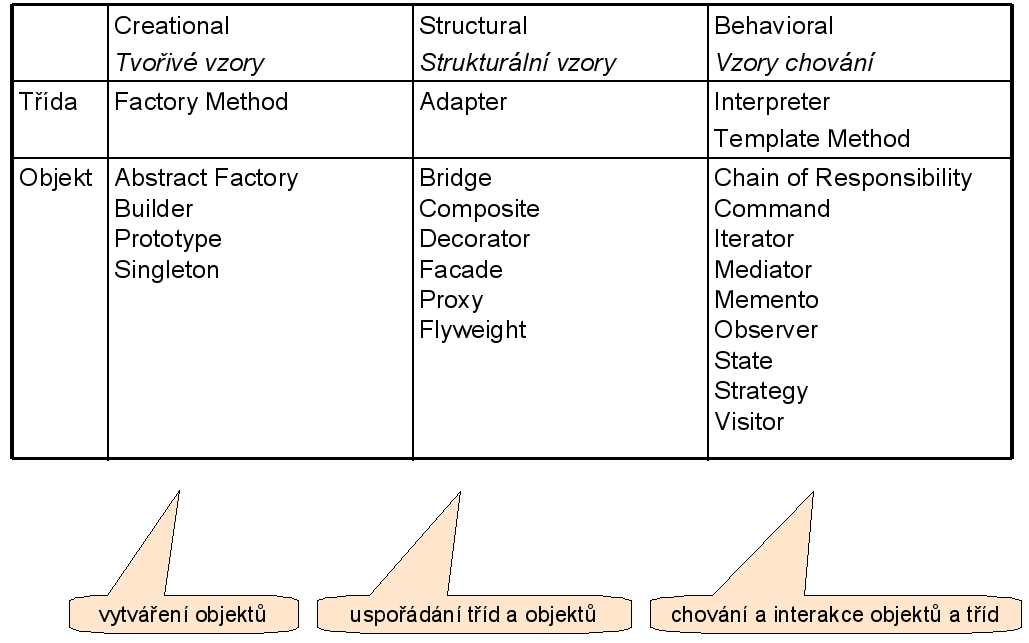
\includegraphics[width=12cm]{informatika/programovanie/obrazky/designpatterns.png}\end{center}
	
	Návrhové vzory je možno klasifikovat dle problémů které řeší. Príklady klasifikace vzorů podle řešených problémů:
	\begin{pitemize}
		\item \emph{Fundamental patterns}: ??? nevyhodíme to, je to jen na wiki a nepopsane
		\item \emph{Creation patterns}: vytváření objektů
		\item \emph{Structural patterns}: jak jsou třídy a objekty složený do větších struktur
		\item \emph{Behavioral patterns}: rozdělení funkčnosti a zodpovědnosti mezi objekty; komunikace mezi objekty; umožňuje zaměřit se při návrhu na propojení tříd, ne na běhové detaily
		\item \emph{Concurrency patterns} ??? tohle taky
	\end{pitemize}
}

\begin{priklady}
Creational patterns:
\begin{pitemize}
    \item Factory method (zajišťuje rozhodnutí o typu vytvářeného objektu při polymorfismu)
    \item Prototype (jak klonovat objekty)
    \item Singleton (jak omezit objekt jen na 1 instanci)
\end{pitemize}

Structural patterns:
\begin{pitemize}
    \item Adapter (konverze rozhraní objektů)
    \item Bridge (oddělení rozhraní a implementace třídy)
    \item Composite (jak složit více objektů do jednoho s jednotným přístupem)
    \item Proxy (jak zajistit přístup k jinému objektu přes můj objekt)
    \item Decorator (jak změnit vlastnosti třídy nebo zajistit rozšířenou funkčnost bez odděďování)
\end{pitemize}

Behavioral patterns:
\begin{pitemize}
    \item Chain of responsibility (jak určit kdo vykoná akci, když z venku přijde požadavek)
    \item Command (odstínění klienta od zpracování požadavku -- klient neurčuje kdy a jak se to provede)
    \item Iterator (projití prvků pole bez znalosti jejich implementace)
    \item Visitor (navštívení všech objektů nějaké struktury a práce s nimi, aby všechny nemusely implementovat stejné metody (a měnit se při jejich změně))
    \item Template (jak mohou odvozené třídy ovlivňovat algoritmy bázové třídy)
\end{pitemize}
\end{priklady}


TODO: rozšíriť, doplniť, opraviť :-)


\section{Architektura počítačů a operačních systémů}
\begin{pozadavky}
\begin{pitemize}
\item Architektury počítače
\item Procesory, multiprocesory
\item Sběrnice, protokoly
\item Vstupní a výstupní zařízení
\item Architektury OS
\item Vztah OS a HW, obsluha přerušení
\item Procesy, vlákna, plánování
\item Synchronizační primitiva, vzájemné vyloučení
\item Zablokování a zotavení z něj
\item Organizace paměti, alokační algoritmy
\item Principy virtuální paměti, stránkování, algoritmy pro výměnu stránek, výpadek stránky, stránkovací tabulky, segmentace
\item Systémy souborů, adresářové struktury
\item Bezpečnost, autentifikace, autorizace, přístupová práva
\item Druhy útoků a obrana proti nim
\item Kryptografické algoritmy a protokoly
\end{pitemize}
\end{pozadavky}
\subsection{Architektury počítače}

\begin{definiceN}{Architektura počítača}
Architektura počítača popisuje \uv{všetko, čo by mal vedieť ten, ktorý programuje v assembleri / tvorí operačný systém}. Teda:
\begin{pitemize}
	\item z akých častí -- štruktúra počítača, usporadanie
	\item význam častí -- funkcia časti, ich vnútorná štruktúra
	\item ako spolu časti komunikujú -- riadenie komukácie
	\item ako sa jednotlivé časti ovládajú, aká je ich funkčnosť navonok
\end{pitemize}
\end{definiceN}

\begin{definiceN}{Víceúrovňová organizace počítače}
\begin{pitemize}
	\item Mikroprogramová úroveň (priamo technické vybavenie počítača)
	\item Strojový jazyk počítače (virtuálny stroj nad obvodovým riešením; vybavenie~-- popis architektúry a organizácie)
	\item Úroveň operačního systému (doplnenie predchádzajúcej úrovne o súbor makroinštrukcií a novú organizáciu pamäti)
	\item Úroveň assembleru (najnižšia úroveň ľudsky orientovaného jazyka)
	\item Úroveň vyšších programovacích jazyků (obecné alebo problémovo orientované; prvá nestrojovo orientovaná úroveň)
	\item Úroveň aplikačních programů
\end{pitemize}
\end{definiceN}


\begin{obecne}{Je teda potrebné definovať}
\begin{pitemize}
	\item Inštrukčný súbor (definícia prechodovej funkcie medzi stavmi počítača, formát inštrukcie, spôsob zápisu, možnosti adresovania operandov)
	\item Registrový model (rozlišovanie registrov procesoru: podľa voľby, pomocou určenia registru~-- explicitný/implicitný register; podľa funkcie registru~-- riadiaci~register/register~operandu)
	\item Definice specializovaných jednotek (jednotka na výpočet vo floatoch;\\fetch/decode/execute jednotky)
	\item Paralelismy (rozklad na úlohy, ktoré sa dajú spracovať súčasne~-- granularita (programy, podprogramy, inštrukcie...))
	\item Stupeň predikce (schopnosť pripraviť sa na očakávanú udalosť (načítanie inštrukcie, nastavenie prenosu dát)~-- explicitná predikcia, štatistika, heuristiky, adaptívna predikcia)

\bigskip
	\item Datové struktury a reprezentáciu dát (spôsob uloženia dát v počítači, mapovacie funkcie medzi reálnym svetom a vnútorným uložením, minimálna a maximálna veľkosť adresovateľné jednotky)
	\item Adresové konvencie (ako sa pristupuje k dátovým štruktúram~-- \emph{segment+offset} alebo \emph{lineárna adresácia}; veľkosť pamäti a jej šírika, \uv{povolené} miesta)

\bigskip
	\item Řízení (spolupráca procesoru a ostatných jednotiek, interakcia s okolím, prerušenia~-- vnútorne/vonkajšie)
	\item Vstupy a výstupy (metódy prenosu dát medzi procesorom a ostatnými jednotkami/počítačom a okolím; zahrňuje definície dátových štruktúr, identifikácia zdroja/cieľa, dátových ciest, protokoly, reakcie na chyby).
	\item Šíře datových cest
	\item Stupeň sdílení (na úrovni obvodov~-- zdieľanie obvodov procesoru a IO; na úrovni jednotiek~-- zdieľanie ALU viacerými procesormi)
\end{pitemize}
\end{obecne}

\subsubsection*{Základní dvě architektury počítačů}

\begin{obecne}{Von Neumannova}
  \begin{pitemize}
      \item Počítač se skládá z řídící jednotky, ALU, paměti a I/O jednotek
      \item Štruktúra počítača sa nemení typom úlohy (tj. počítač je programovaný obsahem paměti). %to tuetschek sorry neumim cist... ajs
      \item Program se nejprve zavede do paměti, z ní se postupně popořadě vybírají instrukce (a následující krok závisí na předchozím), pořadí lze změnit instrukcemi skoku. 
      \item Do jedné paměti, dělené na buňky stejné velikosti, se ukládají i zpracovávaná data. Data jsou reprezentovaná binárně. 
      \item V každém okamžiku je vykonávána jen jedna činnost. Je to architektura SISD (viz Flynnova taxonomie).
  \end{pitemize}

  Je pevně daná instrukční sada. Strojová instrukce obsahuje operační znak, který určuje druh operace, počet parametrů atd., a operandovú část~-- umístnění jednotlivých operandů. Vykonat jednu instrukci znamená:
  \begin{pitemize}
	  \item (fetch) načítať inštrukciu z pamäti do procesoru
	  \item (decode) zistiť o akú inštrukciu ide
	  \item (load) pripraviť zdrojové operandy
	  \item (execute) vykonať operáciu
	  \item (store) uloziť cieľové operandy
  \end{pitemize}

  Při vykonávání programu jsou potřebné různé registry~-- nejdůležitější jsou: PC (Program Counter, obsahuje adresu následující instrukce), IR (Instruction Register, adresa právě vykonávané instrukce), SP (Stack Pointer, ukazatel na vrchol zásobníku), MAR (memory access register~-- adresa do operační paměti), MBR (memory buffer register, dáta čítána/zapisována do paměti).

  Struktura jednoprocesorového počítače podle Von Neumanna:
  \begin{center}
    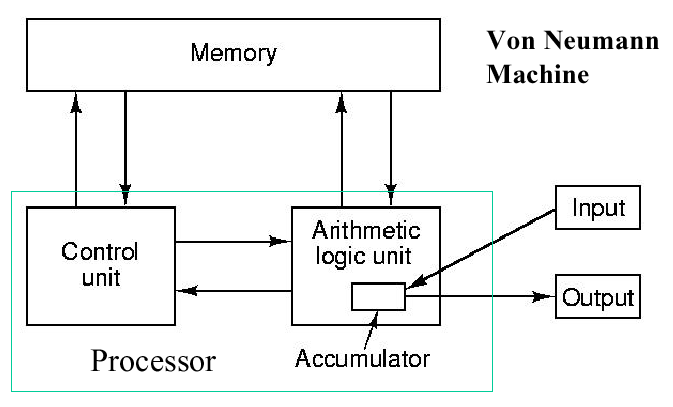
\includegraphics[width=8cm]{informatika/operacne_systemy_a_hw/obrazky/VonNeumann.png}
  \end{center}
\end{obecne}

\begin{obecne}{Harvardská}
Vytvořena až po Von Neumannově, liší se hlavně tím, že program se ukládá do jiné paměti než data (tzn. jsou 2 \uv{druhy paměti}~-- instrukcí a dat). Příklady jsou DSP procesory a mikrokontrolery (např. AVR od Atmelu, a PIC~-- mají paměť na program a data a RISC instrukční sadu; výhoda oddělených pamětí je, že můžou mít různou bitovou hloubku~-- 8 bitové data, ale 12-, 14- či 16- bitové instrukce (např. ARM musí občas použít více než jednou instrukci na zpracování obsahu plné velikosti)).

Oproti Von Neumannově nehrozí nebezpečí přepsání programu sebou samým, ale kvůli většímu počtu paměťových sběrnic je náročnější na výrobu. Paměť navíc nelze dělit podle potřeby (rozdělení je už dané).
\end{obecne}

\subsection{Procesory, multiprocesory}

\begin{definiceN}{Procesor} 
Procesor (CPU – central processing unit) je ústřední výkonnou jednotkou počítače, která čte z paměti instrukce a na jejich základě vykonává program.

Základnými súčasťami procesora sú:
\begin{pitemize}
	\item řadič nebo řídicí jednotka, která řídí tok programu, tj. načítání instrukcí, jejich dekódování, načítání operandů instrukcí z operační paměti a ukládání výsledků zpracování instrukcí
	\item sada registrů k uchování operandů a mezivýsledků.
	\item jedna nebo více aritmeticko-logických jednotek (ALU), které provádí s daty aritmetické a logické operace.
	\item některé procesory obsahují jednu nebo několik jednotek plovoucí čárky (FPU), které provádí operace v plovoucí řádové čárce.
\end{pitemize}
\end{definiceN}

\begin{poznamka}
Súčasné procesory navyše často obsahujú ďalšie rozsiahle funkčné bloky (cache, rôzne periférie)~-- ktoré z \uv{ortodoxného hladiska} nie sú priamo súčasťou \emph{jadra procesoru}. Niektoré procesory môžu obsahovať viac jadier (+logiku slúžiacu k ich vzájomnému prepojeniu). Ďalším trendom je SoC (System on Chip), kde sa na čipe procesora nachádzajú aj ďalšie subsystémy napr. na spracovanie zvuku, grafiky alebo pripojenie externých periférií (takéto riešenia sa využívajú väčšinou v PDA, domácej elektronike, mobiloch atď.).
\end{poznamka}

\begin{obecne}{Dělení podle instruční sady}
Podľa inštrukčnej sady je možné procesory rozdeliť na:
\begin{pitemize}
	\item \textbf{CISC} (Complex Instruction Set Computer): poskytuje rozsiahlu inštrukčnú sadu spolu s rôznymi variantami inštrukcií. Jedna inštrukcia napr. môže vykonať veľa low-level operácií (načítanie z pamäti, vykonať aritmetickú operáciu a výsledok uložiť). Takéto inštrukcie zjednodušovali zápis programov (inštrukcie boli bližšie vyšším programovacím jazykom) a zmenšovali veľkosť programu a počet prístupov do pamäti~-- čo bolo v 60tych rokoch dôležité. Avšak nie vždy je vykonanie jednej zložitej operácie rýchlejšie ako vykonanie viac menej zložitých miesto toho (napr. kvôli zložitému dekódovaniu a použitiu mikrokódu na volanie jednoduchých \uv{podinštrukcií}). Príkladmi CISC architektúr procesorov sú System/360, Motorola 68000 a Intel x86. V súčasnosti napr. x86 rozkladá zložité inštrukcie na \uv{micro-operations} ktoré môžu byť pipeline-ou spracované paralelne a vyšší výkon je tak dosahovaný na väčšom rozsahu inštrukcií. Vďaka tomu sú súčasné x86 procesory minimálne rovnako výkonné ako ozajstné RISC architektúry.
	\item \textbf{RISC} (Reduced Instruction Set Computer): design CPU ktorý uprednosňuje jednoduchšiu inštrukčnú sadu a menšiu zložitosť adresovacích modelov~-- vďaka čomu je možné dosiahnuť lacnejšiu implementáciu, väčšiu úroveň paralelizmu a účinnejšie kompilátory. Dôvodom vzniku bolo aj nevyužívanie celej CISC inštrukčnej sady a upredňostňovania len obmedzenej podmnožiny (designéri procesorov potom optimalizovali len tieto podmnožiny a tak sa zvyšné inštrukcie používali ešte menej...). Kvôli väčšiemu počtu inštrukcií však musia RISC procesory častejšie pristupovať k pamäti... Príkladmi RISC procesorov sú napr. SPARC a ARM. V architekturách typu \textbf{Post-RISC} jde o spojení RISCových vlastností s technikami zvýšení výkonu, jako je out-of-order vykonávání a paralelismus.
    \item \textbf{VLIW}: Very Long Instruction Word or VLIW refers to a CPU architecture designed to take advantage of instruction level parallelism (ILP). A processor that executes every instruction one after the other (i.e. a non-pipelined scalar architecture) may use processor resources inefficiently, potentially leading to poor performance. The performance can be improved by executing different sub-steps of sequential instructions simultaneously (this is pipelining), or even executing multiple instructions entirely simultaneously as in superscalar architectures. The VLIW approach, on the other hand, executes operation in parallel based on a fixed schedule determined when programs are compiled. Since determining the order of execution of operations (including which operations can execute simultaneously) is handled by the compiler, the processor does not need the scheduling hardware that the three techniques described above require. As a result, VLIW CPUs offer significant computational power with less hardware complexity (but greater compiler complexity) than is associated with most superscalar CPUs.
    \item \textbf{EPIC}: (Někdy označován za poddruh VLIW) Explicitly Parallel Instruction Computing (EPIC) is a computing paradigm that began to be researched in the 1990s. This paradigm is also called Independence architectures. It was used by Intel and HP in the development of Intel’s IA-64 architecture, and has been implemented in Intel’s Itanium and Itanium 2 line of server processors. The goal of EPIC was to increase the ability of microprocessors to execute software instructions in parallel, by using the compiler, rather than complex on-die circuitry, to identify and leverage opportunities for parallel execution. This would allow performance to be scaled more rapidly in future processor designs, without resorting to ever-higher clock frequencies, which have since become problematic due to associated power and cooling issues.
\end{pitemize}
\medskip
TODO: asi opravit, možná zpřesnit VLIW a EPIC a určitě přeložit

\medskip
Řekneme, že procesor má \emph{ortogonální instrukční sadu}, pokud žádná instrukce nepředpokládá implicitně použití některých registrů. To umožňuje jednodušší práci algoritmům přidělování registrů v překladačích. Příkladem neortogonální instrukční sady je i x86.
\end{obecne}

\begin{obecne}{Další dělení}
Ďalej je možné procesory rozdeliť podľa dĺžky operandov v bitoch (8, 16, 32, 64...), ktorý je procesor schopný spracovať v jednom kroku. V embedded zariadeniach sa najčastejšie používajú 4- a 8-bitové procesory. V PDA, mobiloch a videohrách 8 resp. 16 bitové. 32 a viac bitov využíajú napr. osobné počítače a laserové tlačiarne.

Dôležitou vlastnosťou je aj taktovacia frekvencia jadra, MIPS (millions of instructions per second) a jeho rýchlosť. V súčasnosti je ťažké dávať do súvislosti výkon procesorov s ich frekvenciou (resp. MIPS)~-- kým Pentium zvládne na výpočet vo floatoch, jednoduchý 8-bitový PIC na to potrebuje oveľa viac taktov. Ďalším \uv{problémom} je superskalarita procesorov, ktorá im umožňuje vykonať viacero nezávislých inštrukcií počas jedného taktu.
\end{obecne}

\begin{obecne}{Techniky pro zvýšení výkonu}
Zvyšovať výkon (procesorov) je možné viacerými spôsobmi. Najjednoduchším (a najpomalším) typom je Subskalárny CPU (načíta a spracúva len jednu inštrukciu naraz~-- preto musí celý procesor čakať kým vykonávanie inštrukcie skončí; je tak zdržovaný dlhšie trvajúcimi inštrukciami). 

\begin{center}
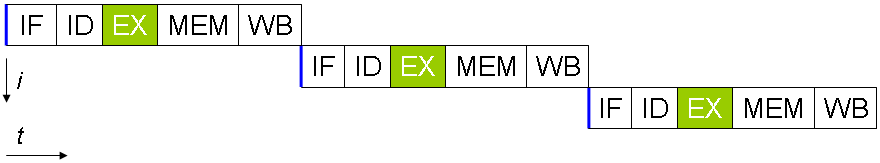
\includegraphics[width=8cm]{informatika/operacne_systemy_a_hw/obrazky/Nopipeline.png}
\end{center}

Pokusy o dosiahnutie skalárneho a lepšieho výkonu vyústili do designov ktoré sa správajú menej lineárne a viac paralelne. Čo sa týka paralelizmu v procesoroch, používajú sa dva druhy pojmov na ich klasifikáciu~-- \emph{Instruction level parallelism} (zvyšovanie rýchlosti vykonávania inštrukcií v procesore a teda zväčšovanie využitia prostriedkov na čipe) a \emph{Thread level parallelism} (zväčšovanie počtu vlákien, ktoré dokáže CPU vykonávať naraz).
\begin{pitemize}
  \item \textbf{pipeline}: 
  Zlepšenie je možné dosiahnúť pomocou \uv{instruction pipelining}-u, ktoré je použíté vo väčšine moderných procesorov. Umožňuje vykonanie viac ako jednej inštrukcie v jednom kroku vďaka rozloženiu spracovávania inštrukcie na viac menších krokov: 
  \begin{center}
  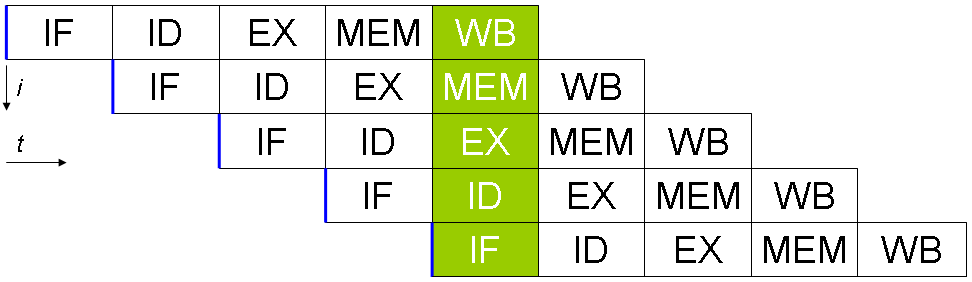
\includegraphics[width=8cm]{informatika/operacne_systemy_a_hw/obrazky/Fivestagespipeline.png}
  \end{center}

  \item \textbf{superskalarita}: Dialša možnosť je použitie superscalar designu, ktorý obsahuje dlhú inštrukčnú pipeline a viacero identických execution jednotiek.  
  \begin{center}
  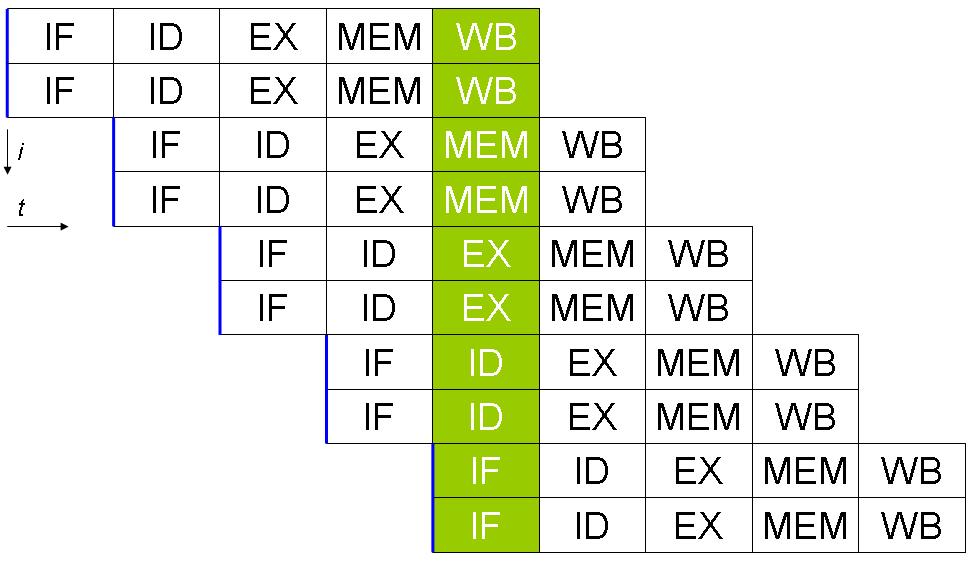
\includegraphics[width=8cm]{informatika/operacne_systemy_a_hw/obrazky/Superscalarpipeline.png}
  \end{center}	

  \item \textbf{Out of order execution}
  \begin{penumerate}
	  \item Načtení instrukce, případně její rozdrobení na mikroinstrukce
	  \item Zařazení do vyčkávací stanice (instruction pool)
	  \item Instrukce čeká na všechny svoje operandy
	  \item Instrukce se vykoná ve své výkonné jednotce (je vybírána z instruction poolu nezávisle na ostatních)
	  \item Výsledky se uchovají ve frontě (reorder buffer)
	  \item Až se všechny starší instrukce zapíší do registrů, zapíše se výsledek této instrukce (opětovné řazení)
  \end{penumerate}

  \item \textbf{Predikce skoků}~-- hluboké pipeliny mají problém, pokud podmíněný skok není proveden; dynamická predicke skoků (historie CPU~-- vzory nějaké hloubky) vs. statická (bez nápovědy~-- skok vpřed se neprovede, skok vzad se provede; s nápovědou~-- překladač odhaduje pravděpodobnost skoku)

  \item \textbf{Spekulativní vykonávaní}~-- vykonávání kódu, který nemusí být zapotřebí; významná disproporce mezi rychlostí CPU a paměti; typické využití je značné předsunutí čtecích operací; CPU provádí i odsouvání zápisových operací


  \item \textbf{Data parallelism}: SIMD inštrukcie (napr. multimediálne inštrukcie), vektorové procesory...
\end{pitemize}
\end{obecne}

\subsubsection*{Multiprocesory}

TODO: jde o copy \& paste z Wiki ... předělat česky/slovensky
\medskip

\begin{definiceN}{Multiprocesor}
  O \emph{multiprocesoru} mluvíme, pokud je použito dvou nebo více procesorů
  (CPU) v rámci jednoho počítačového systému. Termín je také používán mluvíme-li
  o schopnosti systému využívat více procesorů a/nebo schopnosti rozdělovat
  úlohy mezi jednotlivými procesory.
\end{definiceN}

\begin{obecne}{Vztah k datům a instrukcím}
In multiprocessing, the processors can be used to execute a single sequence of instructions in multiple contexts (single-instruction, multiple-data or SIMD, often used in vector processing), multiple sequences of instructions in a single context (multiple-instruction, single-data or MISD, used for redundancy in fail-safe systems and sometimes applied to describe pipelined processors or hyperthreading), or multiple sequences of instructions in multiple contexts (multiple-instruction, multiple-data or MIMD).
\end{obecne}

\begin{obecne}{Symetrie}
In a multiprocessing system, all CPUs may be equal, or some may be reserved for special purposes. A combination of hardware and operating-system software design considerations determine the symmetry (or lack thereof) in a given system. For example, hardware or software considerations may require that only one CPU respond to all hardware interrupts, whereas all other work in the system may be distributed equally among CPUs; or execution of kernel-mode code may be restricted to only one processor (either a specific processor, or only one processor at a time), whereas user-mode code may be executed in any combination of processors. Multiprocessing systems are often easier to design if such restrictions are imposed, but they tend to be less efficient than systems in which all CPUs are utilized equally.

Systems that treat all CPUs equally are called symmetric multiprocessing (SMP) systems. In systems where all CPUs are not equal, system resources may be divided in a number of ways, including asymmetric multiprocessing (ASMP), non-uniform memory access (NUMA) multiprocessing, and clustered multiprocessing (qq.v.).
\end{obecne}

\begin{obecne}{Těsnost spojení multiprocesorů}
\begin{pitemize}
    \item \textbf{Tightly-coupled} multiprocessor systems contain multiple CPUs that are connected at the bus level. These CPUs may have access to a central shared memory (SMP or UMA), or may participate in a memory hierarchy with both local and shared memory (NUMA). The IBM p690 Regatta is an example of a high end SMP system. Intel Xeon processors dominated the multiprocessor market for business PCs and were the only x86 option till the release of AMD's Opteron range of processors in 2004. Both ranges of processors had their own onboard cache but provided access to shared memory; the Xeon processors via a common pipe and the Opteron processors via independent pathways to the system RAM.

    \item \textbf{Chip multiprocessors}, also known as multi-core computing, involves more than one processor placed on a single chip and can be thought of the most extreme form of tightly-coupled multiprocessing. Mainframe systems with multiple processors are often tightly-coupled.

    \item \textbf{Loosely-coupled multiprocessor} systems (often referred to as clusters) are based on multiple standalone single or dual processor commodity computers interconnected via a high speed communication system (Gigabit Ethernet is common). A Linux Beowulf cluster is an example of a loosely-coupled system.
\end{pitemize}
Tightly-coupled systems perform better and are physically smaller than loosely-coupled systems, but have historically required greater initial investments and may depreciate rapidly; nodes in a loosely-coupled system are usually inexpensive commodity computers and can be recycled as independent machines upon retirement from the cluster.

\textbf{SMP} (Symmetric Multiprocessing): viac procesorov so zdieľanou operačnou pamäťou (nutné mechanizmy na zabránenie nesprávnych náhľadov na pamäť a migráciu procesov medzi procesormi). SMP systems allow any processor to work on any task no matter where the data for that task are located in memory; with proper operating system support, SMP systems can easily move tasks between processors to balance the workload efficiently.
\end{obecne}

\subsection{Sběrnice, protokoly}

\begin{pitemize}
	\item \textbf{Struktura sběrnice}: datové linky, adresové linky, řídící linky
	\item \textbf{Synchronní přenos} (vznik události je dán hodinovým signálem) vs. \textbf{asynchronní přenos} (vznik události je určen předcházející událostí~-- napr. signalizáciou začiatku dát) 
	\item \textbf{Parametry sběrnice}: 
	\begin{pitemize}
	  \item \emph{datová šířka}~-- počet přenášených bitů v jednom okamžiku,
	  \item \emph{kapacita}~-- počet bitů přenesených za čas,
	  \item \emph{rychlost}~-- kapacita sběrnice normovaná k jednotce informace. 
	\end{pitemize}  
	\item \textbf{Řízení požadavků}: 
	\begin{pitemize}
	  \item \emph{centrální}~-- náhodné, dle pořadí vzniku požadavků, prioritní,
	  \item \emph{distribuované}~-- kolizní (CSMA/CD), token bus, prioritní linka (daisy chain).
	\end{pitemize} 
	\item \textbf{Přenos dat po sběrnici} může probíhat buď za účasti procesoru (zdroj $\rightarrow$ CPU $\rightarrow$ cíl), nebo bez. Bez procesoru to může být např.:
	\begin{pitemize}
		\item dávkový režim~-- domluva mezi CPU a řadičem na době obsazení sběrnice (napr. pomocou zdvihnutia \uv{lock flagu} na zbernici)
		\item kradení cyklů~-- řadič na dobu přenosu \uv{uspí} procesor (nelze uspat na dlouho, je to technicky náročnější)
		\item transparentní režim~-- řadič rozezná, kdy procesor nepoužívá sběrnici, obvykle nelze větší přenosy najednou
		\item DMA (Direct Memory Access)~-- speciální jednotka pro provádění přenosů dat (mezi zařízeními a pamětí)
	\end{pitemize}
	Jednou z technik, používaných k přenosu dat po sběrnici řadiči DMA, je \emph{scatter-gather}. Znamená to, že v rámci jednoho přenosu se zpracovává víc ne nutně souvislých bloků dat. 
	\begin{pitemize}
	    \item \emph{scatter}~-- DMA řadič v rámci 1 přenosu uloží z 1 místa data na několik různých míst (např hlavičky TCP/IP - jinak zbytečné kopírování)  
	    \item \emph{gather}~-- např. při stránkování paměti - načítání stránek, které fyzicky na disku nemusí být u sebe, složení na 1 místo do paměti.
	\end{pitemize}
\end{pitemize}

Příklady sběrnic:
\begin{pitemize}
	\item ISA, EISA
	\item ATA, ATAPI~-- UltraDMA, Serial-ATA (SATA)
	\item SCSI (Small Computer System Interface)
	\item PCI, PCI-X, PCI Express
	\item AGP (Advanced Graphics Port)
	\item USB (Universal Serial Bus)
	\item FireWire (IEEE 1394)
	\item RS485
	\item $I^{2}C$
\end{pitemize}

Příbuzné sběrnic:
\begin{pitemize}
	\item IrDA
	\item Bluetooth
	\item Wi-Fi, WiMAX 
\end{pitemize}

\subsection{Vstupní a výstupní zařízení}

K I/O zařízením je možné přistupovat dvěma způsoby: pomocí \textbf{port}ů (speciální adresový port CPU) nebo \textbf{pamětovým mapováním} (namapování do fyzické paměti).

Zařízení mají různé charakteristiky:
\begin{pitemize}
	\item \textbf{druh}~-- blokové (disk, síťová karta), znakové (klávesnice, myš)
	\item \textbf{přístup}~-- sekvenční (datová páska), náhodný (hdd, cd)
	\item \textbf{komunikace}~-- synchronní (pracuje s daty na žádost~-- disk), asynchronní (\uv{nevyžádaná} data~-- síťová karta)
	\item \textbf{sdílení}~-- sdílené (preemptivní, lze odebrat~-- síťová karta (po multiplexu OS)), vyhrazené (nepreemptivní~-- tiskárna, sdílení se realizuje přes \emph{spooling}). Reálně se rozdíly stírají.
	\item \textbf{rychlost} (od několika Bps po GBps)
	\item \textbf{směr dat}~-- R/W, R/O (CD-ROM), W/O (tiskárna) 
\end{pitemize}

Přenos dat mezi zařízením a CPU/pamětí:
\begin{pitemize}
	\item \textbf{polling}~-- aktivní čekání na změnu zařízení, přenos provádí CPU
	\item \textbf{přerušení}~-- asynchronní přerušení od zařízení, přenos provádí CPU
	\item \textbf{DMA (Direct Memory Access)}~-- zařízení si samo řídí přístup na sběrnici a přenáší data z/do paměti; po skončení přenosu přerušení (oznámení o dokončení)
\end{pitemize}

Cíle I/O software:
\begin{pitemize}
	\item \textbf{Nezávislost zařízení}~-- programy nemusí dopředu vědět, s jakým přesně zařízením budou pracovat~-- je jedno jestli pracuji se souborem na pevném disku, disketě nebo na CD-ROM
	\item \textbf{Jednotné pojmenování} (na UNIXu /dev)
	\item \textbf{Připojení (mount)}~-- časté u vyměnitelných zařízení (disketa); možné i u pevných zařízení (disk); nutné pro správnou funkci cache OS
	\item \textbf{Obsluha chyb}~-- v mnoha případech oprava bez vědomí uživatele (velmi často způsobeno právě uživatelem)
\end{pitemize}

\subsection{Architektury OS}

\begin{obecne}{Klasická struktura~-- monolitická}
Nejstarší, už IBM 360, Unix, Win., všechny služby uvnitř, prováděny ve chráněném módu, jádro poměrně velké, \uv{údajně} nejrychlejší. Program zavolá službu OS, přes tabulku se zjistí adresa přísl. fce, ta se zavolá a vrátí výsledek.  Nevýhoda: horší údržba -- je-li v programu chyba, může poškodit zbývající části systému, rozšiřování za běhu je komplikované. 
\end{obecne}

\begin{obecne}{Virtuální stroje}
Původní nápad : Virtual Machine pro IBM360 -- oddělit multitasking od OS jako ext. stroj. Nad HW byla další vrstva -- \uv{Virtual Machine} -- měla plánovat, vyrábí pro procesy iluzi holého HW; dneska např. VMWare dělá to samé. Pro IBM360 se dalo použít v kombinaci s CMS (jednoúlohový) i původního OS360 (rychlejší než OS360 na holém HW). 

Dnes: definuji abstraktní stroj, pro něj překládám programy (.NET, Java) $\rightarrow$ přenositelnost, kompatibilita (IBM AS400~-- desítky let), problém~-- pomalé. 
\end{obecne}

\begin{obecne}{Mikrojádro}
snaha aby část běžící v kernel módu byla co nejmenší (třeba jen cca 10 KB), nejnovější, experimentální, často pro Distribuované OS (dnes už nepoužívané), hodně procesů \& komunikace (klient/server), mikrojádro řeší jenom komunikaci. 

Filesystém apod. jsou procesy -- aplikace jim posílají přes jádro požadavky. Jediný komerční OS -- Chorus (ústředny). výhoda: když něco spadne, nepoškodí to zbytek, moduly jdou měnit za běhu, komunikace jde snadno rozšířit na komunikaci po síti. 
\end{obecne}

\begin{obecne}{Architektura WinNT}
  Jádro je poměrně malé (cca 1MB), schopné (pro vyšší vrstvy jsou některé schopnosti skryté), na jeho vzniku se podíleli schopní Unixáři. Byla zde snaha o malou velikost, přenositelnost. Jádro je neutrální vzhledem k vyšším vrstvám, nad ním lze vybudovat různé systémy (Windows subsystém, POSIX, OS/2).

  Rozhraní OS a uživ. programů zajišťuje WinAPI, nad ním se nacházejí různé DLL, mezi kernelem a HW je \uv{hardware abstraction layer}, tj. kernel lze jednoduše upravit pro jiné architektury (Alpha, IA-64).
  Grafické drivery jediné mají přímý přístup k HW (kvůli výkonu), části API (USER, GDI) jsou implementované v jádře, přechod mezi user a kernel režimem zajišťuje ntdll.dll (a je tedy využíván všemi programy). Veškeré služby a aplikace běží v user módu nad jádrem.

  \begin{center}
    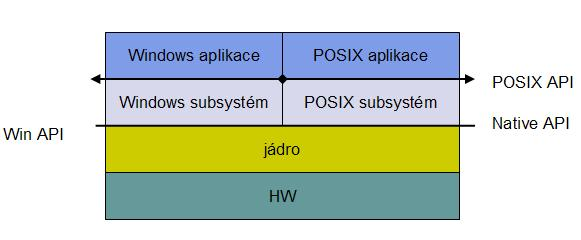
\includegraphics[width=8cm]{informatika/operacne_systemy_a_hw/obrazky/arch-windows.jpg}
  \end{center}
\end{obecne}

\begin{obecne}{Architektura Linuxu}
  \begin{pitemize}
      \item Na úrovni SW -- přenositelnost; abstrakce HW. 
      \item nad HW~-- kernel, nad ním systémová volání, hodně podobné Windows.
  \end{pitemize}

  \begin{center}
    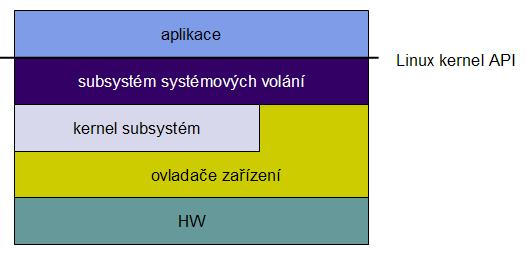
\includegraphics[width=8cm]{informatika/operacne_systemy_a_hw/obrazky/arch-linux.jpg}
  \end{center}
\end{obecne}

\subsection{Vztah OS a HW, obsluha přerušení}

\begin{obecne}{Zjištění změny stavu I/O zařízení:}
\begin{pitemize}
	\item \emph{asynchronní přerušení}~-- zašle zařízení
	\item \emph{polling}~-- peridická kontrola stavu zařízení
\end{pitemize}
\end{obecne}

\begin{obecne}{Druhy přerušení:}
\begin{pitemize}
	\item \emph{synchronní}~-- záměrně (instrukce TRAP~-- vstup do OS), výjimky (nesprávné chování procesu)~-- zpracuje se okamžitě
	\item \emph{asynchronní}~-- vnější událost (např. příchod dat)~-- zpracuje se po dokončení aktuální instrukce 
\end{pitemize}
\end{obecne}

\begin{obecne}{Obsluha přerušení:}
\begin{pitemize}
	\item OS se ujme řízení
	\item uloží se stav CPU (obsah registrů, čítač, ...)
	\item analyzuje se přerušení, vyvolá se příslušná obsluha (pokud není přerušení blokováno)
	\item obslouží se přerušení (např. se zavolá obslužná procedura)
	\item obnoví se stav CPU a aplikace pokračuje, popř. může dojít k přeplánování 
\end{pitemize}
\end{obecne}

\begin{obecne}{I/O software (vrstvy):}
\begin{pitemize}
	\item uživatelský I/O software
	\item I/O nezávislý subsystém
	\item ovladače zařízení
	\item obsluha přerušení 
\end{pitemize}
\end{obecne}

\begin{obecne}{Cíle I/O software:}
\begin{pitemize}
	\item nezávislost zařízení~-- programy nemusí vědět, s jakým přesně pracují
	\item jednotné pojmenování (/dev)
	\item připojení (mount)~-- vyměnitelná zařízení
	\item obsluha chyb
\end{pitemize}
\end{obecne}

\subsection{Procesy, vlákna, plánování}

\subsubsection*{Procesy a vlákna}
Systémové volání je interface mezi OS (kernelspace) a užívatelskými programy (userspace).

\begin{definiceN}{Proces}
  \emph{Proces} je inštancia vykonávaného programu. Kým program je len súbor
  inštrukcií, proces je vlastný \uv{výkon} týchto inštrukcií. Proces má vlastný
  adresný priestor (pamäť), prostriedky, práva a napr. aj ID (Process ID).
\end{definiceN}

Počas života sa môže proces nachádzať v rôznych stavoch:
\begin{pitemize}
  \item \emph{bežiaci}~-- jeden proces na procesor,
  \item \emph{blokovaný}~-- pri použití blokujúceho volania~-- I/O disku atď.,
  \item \emph{pripravený}~-- skončilo blokovanie; spotreboval všetok pridelený čas resp. vrátil riadenie systému, čaká na nové pridelenie procesora,
  \item \emph{zombie}~-- po ukončení procesu, keď už nepracuje~-- ale ešte nebol vymazaný.
\end{pitemize}

\begin{definiceN}{Vlákno}
  \emph{Vlákno} je možnosť pre program ako sa \uv{rozdeliť} na dva alebo viac
  zároveň (resp. pseudo-zároveň) vykonávaných úloh. Oproti procesu mu nie je
  pridelená vlastná pamäť~-- je to len miesto vykonávania inštrukcií v programe.
  Oproti procesu sú jeho \uv{atribútmi} len hodnota programového čítača, stav
  registrov CPU a zásobník.
\end{definiceN}

Oproti Windows/Solaris neobsahuje Linux priamu podporu pre vlákna. Miesto toho podporuje procesy (zhodou okolností :-)) zdieľajúce pamäť. V samotnom jadre linuxu ale vlákna existujú (kthreads).

\subsubsection*{Plánovanie}

Prideľovanie procesorového času jednotlivým procesom má na starosti \emph{plánovač}. Plánovanie pritom môže byť preemptívne alebo nepreemptívne (kooperatívne~-- alla Win16).

\begin{obecne}{Ciele plánovania (niektoré z nich sú očividne protichodné):}
\begin{pitemize}
	\item Spravodlivosť (každy procesor dostane adekvátnu časť času CPU)
	\item Efektívnosť (plne vyťažený procesor)
	\item Minimálna doba odpovede
	\item Průchodnost (maximálny počet spracovaných procesov)
	\item Minimálna réžia systému
\end{pitemize}
\end{obecne}

\begin{obecne}{Kritériá plánovania:}
\begin{pitemize}
	\item Viazanosť procesu na dané CPU a I/O (presun procesu na iný procesor zaberie veľa prostriedkov)
	\item Proces je dávkovy/interaktívny?
	\item Priorita procesu (statická (nemenná~-- okrem \uv{renice}) + dynamická, ktorá sa mení v čase kvôli spravodlivosti)
	\item Ako často proces generuje výpadky stránok (nejaký popis???)
	\item Kolik skutočného času CPU proces obdržel
\end{pitemize}
\end{obecne}

\begin{obecne}{Algoritmy:}
\begin{pitemize}
	\item \textbf{FIFO}: nepreemptívny, proces opustí procesor až po skončení

	\item \textbf{Round Robin}: preemptívne rozšírenie FIFO, po skončení časového kvanta je proces presunutý na koniec fronty

	\item \textbf{Plánovanie s viacerými frontami}: niekoľko front, procesu z $i$-tej fronty je pridelený procesor až keď vo frontách $1, \dots, i-1$ nie je pripravený ziadny proces. Ak proces skončil I/O operáciou, je blokovaný a presunutý do fronty $i-1$, ak skončil preempciou, je pripravený a presunutý do fronty $i+1$.

	\item \textbf{SMP}: fronta CPU čakajúcich na pripravené procesy (aktívne (spotrebováva energiu) vs. pasívne čakanie (špeciálne inštrukcie)), \uv{vzťah}/afinita procesov k CPU

	\item TODO: Plánovanie windows vs. linux???
\end{pitemize}
\end{obecne}

\subsection{Synchronizační primitiva, vzájemné vyloučení}

\subsubsection*{Pojmy}

\emph{Race conditions}: výsledek operace závisí na plánování

\emph{Vzájemné vyloučení (mutual exclusion)}: kritickou operaci provádí nejvýše jeden proces. Podmínky vzájemného vyloučení:
\begin{penumerate}
	\item Žádné dva procesy nemohou být najednou ve stejné kritické sekci
	\item Nemohou být učiněny žádné předpoklady o rychlosti nebo počtu CPU
	\item Žádný proces mimo kritickou sekci nesmí blokovat jiný proces
	\item Žádný proces nesmí čekat nekonečně dlouho v kritické sekci
\end{penumerate}

\emph{Kritická sekce}: část programu, kde se provádí kritická operace

Metody dosáhnutí vzájemného vyloučení: aktivní čekání (busy waiting) a pasivní čekání/blokování.

\subsubsection*{Aktivní čekání}
\emph{Vlastnosti}: spotřebovává čas procesoru, vhodnější pro předpokládané krátké doby čekání, nespotřebovává prostředky OS, rychlejší.

Je možné použít např. \emph{zakázání přerušení} (vhodné pro jádro OS). Používání \emph{zámků} nefunguje:
\begin{verbatim}
int lock;
void proc(void) {
  for (;;) {
    nekritická_sekce();
    while (lock != 0);
    lock = 1;
    kritická_sekce();
    lock = 0;
  }
}
\end{verbatim}
ale \emph{důsledné střídání} ano (to ale porušuje podmínku 3.)

\begin{verbatim}
int turn = 0;

void p1(void)                void p2(void)
{                            {
  for (;;) {                   for (;;) {
    while (turn != 0);           while (turn != 1);
    kritická_sekce();            kritická_sekce();
    turn = 1;                    turn = 0;
    nekritická_sekce();          nekritická_sekce();
  }                            }
}                            }
\end{verbatim}

\emph{Petersonovo řešení}:
\begin{verbatim}
#define N 2                   /* počet procesů */
 
int turn;
int interested[N];            /* kdo má zájem */
 
void enter_region(int proc) { /* proc: kdo vstupuje */
int other;
 
  other = 1-proc;             /* číslo opačného procesu */
  interested[proc] = TRUE;    /* mám zájem o vstup */
  turn = proc;                /* nastav příznak */
  while (turn == proc && interested[other] == TRUE);
}
 
void leave_region(int proc) { /* proc: kdo vystupuje */
  interested[proc] = FALSE;   /* už odcházím */
}
\end{verbatim}
 
\emph{Instrukce TSL} (spin-lock) - je nutné aby ji podporoval HW (všechny současné procesory nějakou mají):
\begin{verbatim}
enter_region:
    tsl   R,lock           ; načti zámek do registru R a
                           ; nastav zámek na 1
    cmp   R,#0             ; byl zámek nulový?
    jnz   enter_region     ; byl-li nenulový, znova
    ret                    ; návrat k volajícímu - vstup do
                           ; kritické sekce
 leave_region:
    mov   lock,#0          ; ulož do zámku 0
    ret                    ; návrat k volajícímu
\end{verbatim}

\subsubsection*{Pasivní čekání}
\emph{Vlastnosti}: proces je ve stavu blokován, vhodné pro delší doby čekání, spotřebovává prostředky OS, pomalejší.

Postup používající Sleep/Wakeup (implementovány OS, atomické operace - sleep uspí volající proces, wakeup probudí udaný proces) nefunguje (viď Problém producent/konzument).

\textbf{Semafory}... Sémantika:
\begin{verbatim}
Down(Semaphore s) {
  wait until s > 0, then s := s-1;
  /* must be atomic once s > 0 is detected */
}
\end{verbatim}
(pokud je čítač $>$ 0, sníží čítač o 1 a pokračuje dál; pokud je čítač $=$ 0, operace DOWN se zablokuje a proces je přidán do fronty čekající na tomto semaforu)

\begin{verbatim}
Up(Semaphore s) {
  s := s+1;   /* must be atomic */
}
\end{verbatim}
(pokud je fronta neprázdná, vybere libovolný proces a ten probudí za DOWN; jinak zvětší čítač o 1)

\begin{verbatim}
Init(Semaphore s, Integer v) {
  s := v;
}
\end{verbatim}

Je možné \uv{používať} aj sémantiku, kde sa hodnota vždy zníži/zvýši o 1 (a je možné sa teda dostať do záporných hodnôt semafóru)... Špeciálny (binárny) typ semaforu, kde sú povolené len hodnoty 0 a 1 (v Up sa miesto $s:=s+1$ volá $s:=1$) sa nazýva \emph{mutex} a používa sa na riadenie prístupu k jednej premennej.

\textbf{Monitory}
\par Implementovány překladačem, lze si představit jako třídu C++ (všechny proměnné privátní, funkce mohou být i veřejné), vzájemné vyloučení v jedné instanci (zajištěno synchronizací na vstupu a výstupu do/z veřejných funkcí, synchronizace implementována blokovacím primitivem OS). ???TODO

\textbf{Zprávy}
\par Operace SEND a RECEIVE, zablokování odesílatele/příjemce, adresace proces/mailbox, rendez-vous...

\textbf{RWL - read-write lock}, \textbf{bariéry}...

Ekvivalence primitiv - pomocí jednoho blokovacího primitiva lze implementovat jiné blokovací primitivum.

Rozdíly mezi platformami: Windows - jednotné funkce pro pasivní čekání, čekání na více primitiv, timeouty. Unix - OS implementuje semafor, knihovna pthread.

\subsubsection*{Klasické synchronizační problémy}
\textbf{Problém producent/konzument}
\par Producent vyrába predmety, konzument ich spotrebúva. Medzi nimi je sklad pevnej veľkosti (N). Konzument nemá čo spotrebúvať ak je sklad prázdny; producent prestane vyrábať, ak je sklad plný. 

\begin{verbatim}
int N = 100;
int count = 0;
void producer(void) {
    int item;
    while(TRUE) {
        produce_item(&item);
        if(count==N) sleep ();
        enter_item(item);
        count++;
        if(count == 1) wake(consumer);
    }
}
void consumer(void) {
    int item;
    while(TRUE) {
        if(count==0) sleep ();
        remove_item(&item);
        count--;
        if(count==N-1)
            wake(producer);
        consume_item(&item);
    }
}
\end{verbatim}

\begin{penumerate}
	\item Buffer je prázdny, a konzument práve prečítal count, aby zistil, či je rovný nule
	\item Preplánovanie na producenta
	\item Producent vytvorí item a zvýši count
	\item Producent zistí, či je count rovný jednej. Zistí že áno, čo znamená že konzument bol predtým zablokovaný (pretože muselo byť 0), a zavolá wakeup
	\item Teraz môže dôjsť k zablokovaniu: konzument sa uspí, pretože si myslí, že nemá čo zobrať; producent bude chvíľu produkovať a dôjde "preplneniu" $\Rightarrow$ uspí sa; spí producent aj konzument :o) 
\end{penumerate}

\textbf{Problém obědvajících filosofů}
\par Pět filosofů sedí okolo kulatého stolu. Každý filosof má před sebou talíř špaget a jednu vidličku. Špagety jsou bohužel slizké a je třeba je jíst dvěma vidličkami. Život filosofa sestává z období jídla a období přemýšlení. Když dostane hlad, pokusí se vzít dvě vidličky, když se mu to podaří, nají se a vidličky odloží.

\textbf{Problém ospalého holiče}
\par Holič má ve své oficíně křeslo na holení zákazníka a pevný počet sedaček pro čekající zákazníky. Pokud v oficíně nikdo není, holič se posadí a spí. Pokud přijde první zákazník a holič spí, probudí se a posadí si zákazníka do křesla. Pokud přijde zákazník a holič už střihá a je volné místo v čekárně, posadí se, jinak odejde.

\subsection{Zablokování a zotavení z něj}

Prostředek je cokoliv, k čemu je potřeba hlídat přístup (HW zařízení~-- tiskárny, cpu; informace~-- záznamy v DB). Je možné je rozdělit na \emph{odnímatelné} (lze odejmout procesu bez následků~-- CPU, paměť) a \emph{neodnímatelné} (nelze odejmnout bez nebezpečí selhání výpočtu~-- CD-ROM, tiskárna... tento druh způsobuje problémy).

Práce s prostředky probíhá v několika krocích: \emph{žádost o prostředek} (blokující, právě tady dochází k zablokování), \emph{používání} (např. tisk), \emph{odevzdání} (dobrovolné/při skončení procesu).

Množina procesů je \emph{zablokována}, jestliže každý proces z této množiny čeká na událost, kterou může způsobit pouze jiný proces z této množiny.

\subsubsection*{Coffmanovy podmínky}
Splnenie týchto podmienok je nutné pre zablokovanie:
\begin{penumerate}
	\item \textbf{Vzájemné vyloučení} – každý prostředek je buď vlastněn právě jedním procesem nebo je volný.
	\item \textbf{Drž a čekej} – procesy aktuálně vlastnící nějaké prostředky mohou žádat o další.
	\item \textbf{Neodnímatelnost} – přidělené prostředky nemohou být procesům odebrány.
	\item \textbf{Čekání do kruhu} – existuje kruhový řetěz procesů, kde každý z nich čeká na prostředek vlastněný dalším článkem řetězu.
\end{penumerate}

\subsubsection*{Řešení zablokování}
\begin{pitemize}
	\item \textbf{Pštrosí algoritmus}~-- Zablokování se ani nedetekuje, ani se mu nezabraňuje, ani se neodstraňuje, Uživatel sám rozhodne o řešení (kill). Nespotřebovává prostředky OS~-- nemá režii ani neomezuje podmínky provozu. (Nejčastější řešení~-- Unix, Windows) 
	\item \textbf{Detekce a zotavení}~-- Hledá kružnici v orientovaném grafu (hrany vedou od procesu, který čeká, k procesu, který prostředek vlastní), pokud tam je kružnice, nastalo zablokování a je třeba ho řešit:
		\begin{pitemize}
			\item \emph{Odebrání prostředku}~-- dohled operátora, pouze na přechodnou dobu
			\item \emph{Zabíjení procesů z cyklu} (resp. mimo cyklus vlastnící identický prostředek)
			\item \emph{Rollback} (OS ukládá stav procesů, při zablokování se některé procesy vrátí do předchozího stavu $\Rightarrow$ ztracena práce... obdoba u DB)
		\end{pitemize}
	\item \textbf{Vyhýbání se}~-- Bezpečný stav (procesy/prostředky nejsou zablokovány, existuje cesta, jak uspokojit všechny požadavky na prostředky spouštěním procesů v jistém pořadí); Viď. bankéřův algoritmus. Nutné je předem znát všechny prostředky, které budou programy potřebovat; OS pak dává prostředky tomu, který je nejblíž svému maximu potřeby a navíc pro který je prostředků dost na dokončení. Dnes se moc nepoužívá.
	\item \textbf{Předcházení (prevence)}~-- napadení jedné z Coffmanovy podmínek
		\begin{penumerate}
			\item \emph{Vzájemné vyloučení}~-- \emph{spooling} (prostriedky spravuje jeden systemový proces, ktory dohliada na to, aby jeho stav bol konzistentny (tiskarna)~-- pozor na místo na disku)
			\item \emph{Drž a čekej}~-- žádat o všechny prostředky před startem procesu. Nejprve všechno uvolnit a pak znovu žádat o všechny najednou
			\item \emph{Neodnímatelnost}~-- vede k chaosu
			\item \emph{Čekání do kruhu}~-- nejvýše jeden prostředek~-- všechny prostředky jednoznačně očíslovány, procesy mohou žádat o prostředky jen ve vzestupném pořadí

		\end{penumerate}
			\item \emph{Dvojfázové zamykání}~-- nejprve postupně všechno zamykám (první fáze). Potom se může pracovat se zamčenými prostředky~-- a na závěr se už jen odemyká (druhá fáze)~-- viď transakční spracování u databází ((striktní/konzervativní) dvoufázové zpracování)
\end{pitemize}

\textbf{Bankéřův algoritmus}: Bankéř má klienty a těm slíbil jistou výšku úvěru. Bankéř ví, že ne všichni klienti potřebují plnou výši úvěru najednou. Klienti občas navštíví banku a žádají postupně o prostředky do maximální výšky úvěru. Až klient skončí s obchodem, vrátí bance vypůjčené peníze. Bankéř peníze půjčí pouze tehdy, zůstane-li banka v bezpečném stavu.

\subsection{Organizace paměti, alokační algoritmy}

\textbf{Hierarchie paměti} (směrem odshora dolů roste velikost, cena na bajt a rychlost klesá~-- a naopak\dots):
\begin{pitemize}
    \item \emph{registry CPU} --- 10ky-100vky bajtů (IA-32: obecné registy pár 10tek), IA-64~-- až kB (extrém), stejně rychlé jako CPU. 
    \item \emph{cache} --- z pohledu aplikací není přímo adresovatelná; dnes řádově MB, rozdělení podle účelu, několik vrstev. L1 cache (cca 10ky kB)~-- dělené instrukce/data; L2 (cca MB) sdílené instr\&data, běží na rychlosti CPU (dřív bývala pomalejší), servery~-- L3 (cca 10MB). Vyrovnává rozdíl rychlosti CPU a RAM. Využívá lokality programů -- cyklení na místě; sekvenčního přístupu k datům. Pokud nenajdu co chci v cache -- \uv{cache-miss}, načítá se potřebné z RAM (po blocích), jinak (v 95-7\% případů) nastane \uv{cache-hit}, tj. požadovaná data v cache opravdu jsou a do RAM nemusím.
    \item \emph{hlavní paměť} (RAM) --- přímo adresovatelná procesorem, 100MB~-- GB; pomalejší než CPU; CAS~-- doba přístupu na urč. místo~-- nejvíc zdržuje (v 1 sloupci už čte rychle, dat. tok dostatečný), další~-- latence~-- doba než data dotečou do CPU~-- hraje roli vzdálenost (AMD- integrovaný řadič v CPU) 
    \item \emph{pomocná paměť} --- není přímo adresovatelná, typicky HDD; náh. přístup, ale pomalejší. ~100GB, různé druhy~-- IDE, SATA, SCSI; nejvíc zdržuje přístupová doba (čas seeku) cca 2-10ms; obvykle sektor~-- 512 B; roli hraje i rychlost otáčení (4200~-- 15000 RPM)~-- taky řádově ms. 
    \item \emph{zálohovací paměť} --- nejpomalejší, z teorie největší, dnes ale neplatí; typicky~-- pásky; pro větší kapacitu~-- autoloadery ; sekvenční přístup; dnes~-- kvůli rychlosti často zálohování RAIDem.
\end{pitemize}

\textbf{Správce paměti}: část OS, která spravuje paměťovou hierarchii se nazývá\\správce paměti (memory manager):
\begin{pitemize}
	\item udržuje informace o volné/plné části paměti
	\item stará se o přidělování paměti
	\item a \uv{výměnu paměti s diskem}
\end{pitemize}

\textbf{Přiřazení adresy}
\begin{pitemize}
	\item při překladu (je již známo umístění procesu, generuje se absolutní kód, PS: statické linkování)
	\item při zavádění (OS rozhodne o umístění~-- generuje se kód s relokacemi, PS: dynamické linkování)
	\item za běhu (proces se může stěhovat i za běhu, relokační registr)
\end{pitemize}

\textbf{Overlay}~-- Proces potřebuje více paměti než je skutečně k dispozici.
Programátor tedy rozdělí program na nezávislé části (které s v paměti podle
potřeby vyměňnují) a část nezbytnou pro všechny části\dots

\textbf{Výměna (swapping)}~-- dělá se, protože proces musí být v hlavní paměti,
aby jeho instrukce mohly být vykonávány procesorem... Jde o výměnu obsahu paměti
mezi hlavní a záložní.

\textbf{Překlad adresy}~-- nutný, protože proces pracuje v logickém (virtuálním) adresovém prostoru, ale HW pracuje s fyzickým adresovým prostorem...

\textbf{Spojité přidělování}~-- přidělení jednoho bloku / více pamětových oddílů (\emph{pevně}~-- paměť pevně rozdělena na části pro různé velikosti bloků/\emph{volně}~-- v libovolné části volné paměti může být alokován libovolně veliký blok)

\textbf{Informace o obsazení paměti}~-- bitová mapa / spojový seznam volných bloků (spojování uvolněného bloku se sousedy)

\textbf{Alokační algoritmy}:
\begin{pitemize}
	\item \emph{First-fit}~-- první volný dostatečné velikosti~-- rychlý, občas ale rozdělí velkou díru
	\item \emph{Next-fit}~-- další volný dostatečné velikosti~-- jako First-fit, ale rychlejší
	\item \emph{Best-fit}~-- nejmenší volný dostatečné velikosti~-- pomalý (prohledává celý seznam), zanechává malinké díry (ale nechává velké díry vcelku)
	\item \emph{Worst-fit}~-- největší volný~-- pomalý (prohledává celý seznam), rozdělí velké díry
	\item \emph{Buddy systém}~-- paměť rozdělena na bloky o velikosti $2^n$, bloky stejné velikosti v seznamu, při přidělení zaokrouhlit na nejbližší $2^n$, pokud není volný, rozštípnou se větší bloky na příslušné menší velikosti, při uvolnění paměti se slučují sousední bloky (buddy)
\end{pitemize}

\textbf{Fragmentace paměti}:
\begin{pitemize}
	\item \emph{externí}~-- volný prostor rozdělen na malé kousky, pravidlo 50\% -- po nějaké době běhu programu bude cca 50\% paměti fragmentováno a u toho to zůstává
	\item \emph{interní}~-- nevyužití celého přiděleného prostoru
	\item \emph{sesypání}~-- pouze při přiřazení adresy za běhu, nebo segmentaci~-- nelze při statickém přidělení adresy
\end{pitemize}

\subsection{Principy virtuální paměti, stránkování, algoritmy pro výměnu stránek, výpadek stránky, stránkovací tabulky, segmentace}

\subsubsection*{Virtuální paměť}
\begin{pitemize}
	\item procesy pracují s virtuální adresou
	\item mapování adresy na fyzickou - mapovací tabulky
	\item obraz virtuální paměti (VAP) částečně v RAM a částečně na disku
	\item dříve iluze větší paměti, dnes hlavně ochrana přístupu
	\item stránkování / segmentace 
\end{pitemize}

\subsubsection*{Stránkování}
podporované všemi velkými CPU a OS, jednorozměrný VAP
\begin{pitemize}
	\item VAP rozdělen na stránky (velikost je mocnina 2), FAP na rámce (úseky stejné délky)
	\item převod stránkovací tabulkou, příznak existence mapování (výpadek stránky $\rightarrow$ synchronní přerušení)
		\par \begin{center}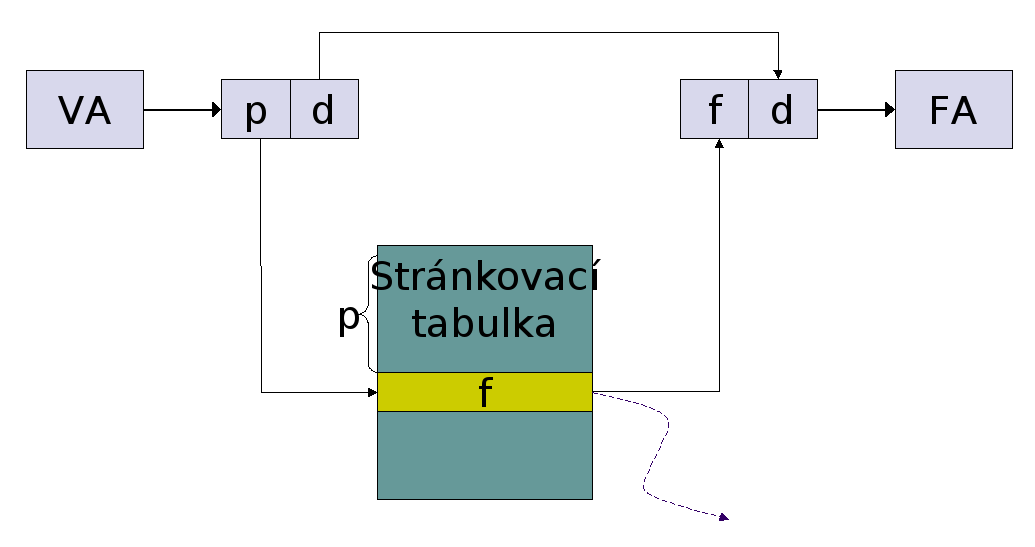
\includegraphics[width=10cm]{informatika/operacne_systemy_a_hw/obrazky/strankovani1.png}\end{center}
	\item umožnuje \emph{oddělené VAP} i \emph{sdílenou paměť} - mapování virtuální stránky 2 procesů na jednu fyzickou
	\item víceúrovňové stránkování (např. kvůli velikosti)
		\par \begin{center} 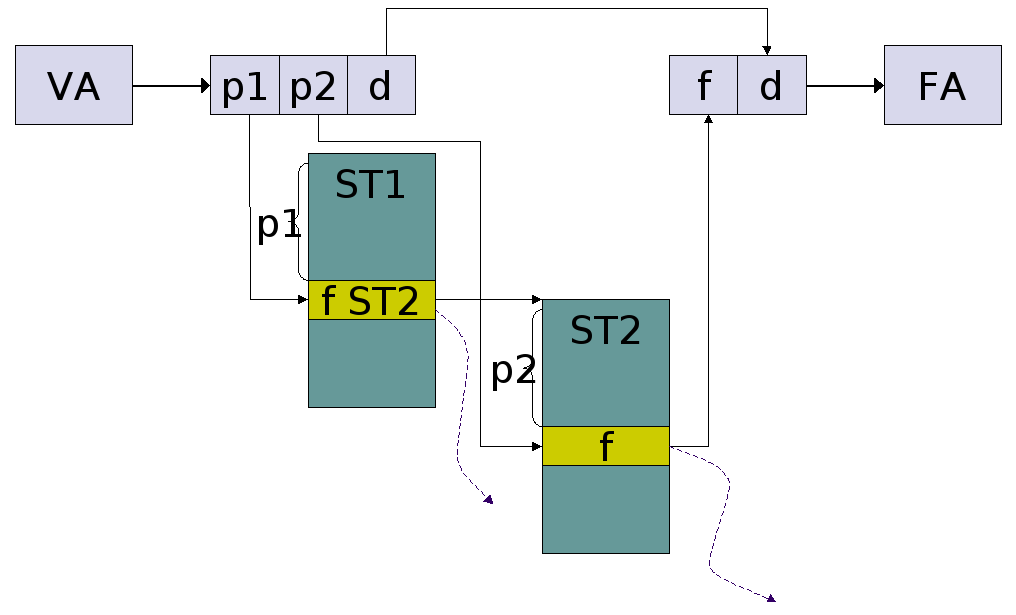
\includegraphics[width=10cm]{informatika/operacne_systemy_a_hw/obrazky/strankovani2.png} \end{center}
	\item TLB (Translation Lookaside Buffer) - asociativní paměť sloužící na rychlé vyhledání mapování virtuální stránky na fyzickou, využívá lokalitu chování programů
		\par \begin{center} 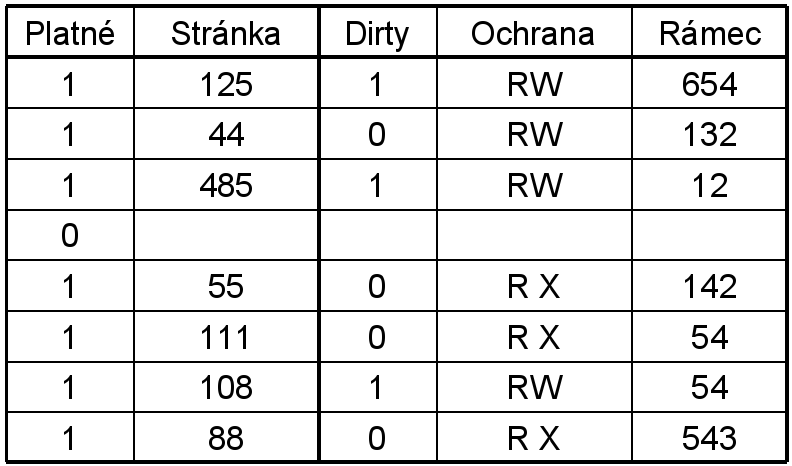
\includegraphics[width=6cm]{informatika/operacne_systemy_a_hw/obrazky/strankovani-tlb.png} \end{center} 
		\par ...nulaúrovňové stránkování - používá pouze TLB, řízeno také OS (oblíbené u 64-bitových CPU - UltraSPARC III)
	\item inverzní stránkování (např. když FAP je menší než VAP, 64-bitové CPU - IA-64)
		\par \begin{center} 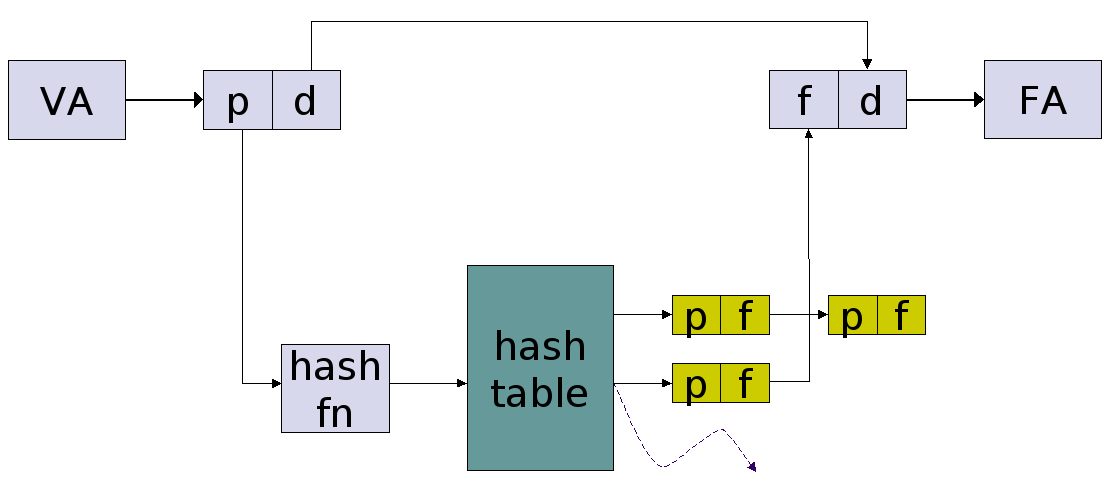
\includegraphics[width=10cm]{informatika/operacne_systemy_a_hw/obrazky/strankovani-inv.png} \end{center} 
\end{pitemize}

Akce vykonávané při výpadku stránky:
\begin{pitemize}
	\item výjimka procesoru
	\item uložit stav CPU (kontext)
	\item zjistit VA
	\item kontrola platnosti adresy a práv
	\item nalezení volného rámce
	\item zrušit mapování na nalezený rámec
	\item pokud je vyhazovaný rámec vyhazován, spustit ukládání na disk
	\item načíst z disku požadovanou stránku do rámce
	\item zavést mapování
	\item obnovit kontext
\end{pitemize}


Při implementaci stránkování je nutno brat v úvahu: 
\begin{pitemize}
    \item \emph{znovuspuštění instrukce} --- je potřeba aby procesor po výpadku zkusil přístup do paměti znova. dnes umí všechny CPU, např. 68xxx - problémy (přerušení v půlce instrukce) 
    \item \emph{sdílení stránek} --- jednomu rámci odp. víc stránek $\rightarrow$ pokud s ním něco dělám, týká se to všech stránek!  musím vše ost. odmapovat. musím si pamatovat mapování pro každý rámec - obrácené tabulky. 
    \item \emph{odstranění položky z TLB při rušení mapování} --- nestačí změnit tabulky, musí se vyhodit i z TLB (kde to může, ale nemusí být). problém - u multiprocesorů má každá CPU vlastní TLB, tabulky jsou sdílené $\rightarrow$ CPU při rušení mapování musí poslat interrupt s rozkazem ke smazání všem (i sobě), počkat na potvrzení akce od všech.
\end{pitemize}

\subsubsection*{Algoritmy pro výměnu stránek}
\begin{pitemize}
	\item \textbf{Optimální stránka} (v okamžiku výpadku stránky vybírám stránku, na níž se přistoupí za největší počet instrukcí) - nelze implementovat
	\item \textbf{NRU} (Not Recently Used) - každá stránka má příznaky Accessed a Dirty (typicky implementovatelné v HW, možno simulovat SW); jednou za čas se smažou všechna A; při výpadku rozdělím stránky podle A,D a vyberu stránku z nejnižší neprázdné třídy:
		\par \begin{center}
		\begin{tabular}{|c|c|c|}
			\hline 
			  & A & D \\
			\hline
			0 & 0 & 0 \\
			\hline
			1 & 0 & 1 \\
			\hline
			2 & 1 & 0 \\
			\hline
			3 & 1 & 1 \\
			\hline
		\end{tabular}
		\end{center}
	\item \textbf{FIFO} (vykazuje anomálie - Belady (zvětšení počtu výpadků stránky, když zvýšíme počet stránek v paměti)), druhá šance (úprava FIFO; pokud A=1, zařadím na konec FIFO... nevykazuje anomálie)
	\item \textbf{Hodiny} - modifikace druhé šance: kruhový zoznam stránek + iterátor na ukazující na nejstarší stránku v zoznamu. Při výpadku (a neexistenci volého rámce) se zjistí, jestli má *iterator nastavený příznak Accessed. Jestli ne, tato stránka bude nahrazena - v opačném případě se Accessed příznak zruší a iterator++. Toto se opakuje, dokud nedojde k výměně\dots
	\item \textbf{LRU} (Least Recently Used) - často používané stránky v posledním krátkém časovém úšeku budou znovu použity, čítač použití stránek, možné implementovat v HW
	\item \textbf{NFU} (Not Frequently Used) - SW simulace LRU, SW čítač ke každé stránce; jednou za čas projdu všechna A a přičtu je k odpovídajícím čítačům; vybírám stránku s nejnižším čítačem; nezapomíná - je možná modifikace se stárnutím čítače
\end{pitemize}

\subsubsection*{Segmentace}
dnes pouze Intel IA-32, dvojrozměrný VAP
\begin{pitemize}
	\item rozdělení programu na segmenty (napr. podle částí s různými vlastnostmi - kód, data, zásobníky\dots), různé délky segmentů, ktoré můžou měnit svoji délku za běhu
	\item VAP dvourozměrný (segment, offset), FAP jednorozměrný (vyzerá jako při spojitém pridělování paměti)
	\item segmentová převodní tabulka (VA se skládá ze dvou častí S:D, v tabulce se najde adresa segmentu S\dots k této adrese se poté přičte D, co je umístnění adresy v FA), příznak existence mapování
	\item při výpadku je nutné měnit celý segment (ty mohou být velké), je možné segmenty sesypat - ale nelze mít segment větší než FAP
\end{pitemize}

Segmentaci je možné kombinovat se stránkováním (odstraňuje nevýhody segmentace, neprovádí se výpadky segmentů):
\par \begin{center}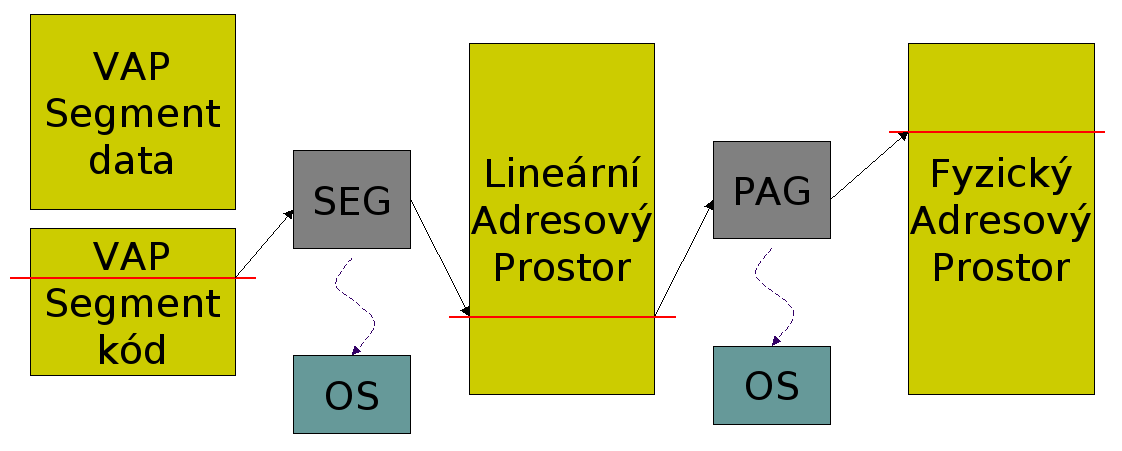
\includegraphics[width=12cm]{informatika/operacne_systemy_a_hw/obrazky/segmentace-a-strankovani.png}\end{center}

\subsection{Systémy souborů, adresářové struktury}

\begin{definiceN}{soubor}
  \emph{Soubor} je pojmenovaná množina souvisejících informací, která leží v
  pomocné paměti (na disku).\\
  \emph{Soubor} je abstrakce, která umožňuje uložit informaci na disk a později ji
  přečíst. Abstrakce odstiňuje uživatele od podrobností práce s disky.
\end{definiceN}

\begin{obecne}{Soubory}
  \begin{pitemize}
    \item pojmenování souboru (umožňuje uživateli přístup k jeho datům;
    přesná pravidla pojmenování určuje OS - malá vs. velká písmenka,
    speciální znaky, délka jména, přípony a jejich význam)
    \item atributy souborů (opět určuje OS) - jméno, typ, umístění, velikost, ochrana, časy, vlastník, \dots
    \item struktura souborů - sekvence bajtů / sekvence záznamů / strom
    \item typy souborů - běžné soubory, adresáře (systémové soubory vytvářející strukturu souborového systému), speciální soubory (znakové/blokové, soft linky)
    \item přístup 
    \begin{pitemize}
      \item \textbf{sekvenční}~-- pohyb pouze vpřed, OS může přednačítat
      \item \textbf{náhodný}~-- možno měnit aktuální pozici
      \item \textbf{paměťově mapované soubory}~-- pojmenovaná virtuální paměť,
      práce se souborem instrukcemi pro práci s pamětí, ušetří se kopírování
      pamětí; mají i problémy (přesná velikost souboru, zvětšování souboru,
      velikost souborů)
    \end{pitemize}
    \item volné místo na disku - bitmapa / spojový seznam volných bloků 
  \end{pitemize}
\end{obecne}

\begin{obecne}{Uložení souborů}
  Soubory se ukládají na disk po blocích
  \begin{pitemize}
    \item souvislá alokace - souvislý sled bloků
    \item spojovaná alokace - blok odkazuje na další
    \item indexová alokace - inode (UNIX) 
  \end{pitemize}
\end{obecne}

\begin{obecne}{Adresáře}
  \begin{pitemize}
    \item zvláštní typ souboru
    \item operace nad adresáři - hledání souboru / vypsání adresáře /
    přejmenování, vytvoření, smazání souboru 
    \item kořen, aktuální adresář, absolutní/relativní cesta
    \item hierarchická struktura 
    \begin{pitemize}
      \item \emph{strom}~-- jednoznačné pojmenování (cesta)
      \item \emph{DAG}~-- víceznačné pojmenování, ale nejsou cykly
      \item \emph{obecný graf}~-- cykly vytváří problém při prohledávání
    \end{pitemize}
    \item implementace adresářů - záznamy pevné velikosti, spojový seznam, B-stromy 
  \end{pitemize}
\end{obecne}

\begin{obecne}{Co musí filesystém umět?}
musí splňovat 3 věci: \emph{správu souborů} (kde jsou, jak velké), \emph{správu adresářů} (převod jméno $\leftrightarrow$ id) (někdy to dělá jiný prostředek, dnes větš. umí FS sám), \emph{správu volného místa}. někdy mohou být i další (odolnost proti výpadkům) 

Velikost bloků -- blok = nejmenší jednotka pro práci s diskem; disk pracuje s min. 1 sektorem (typicky 512 B) - někdy by pak bylo moc bloků $\rightarrow$ OS sdruží několik sektorů lineáně vedle sebe = 1 blok. velikost: velké = rychlejší práce, ale vnitřní fragmentace (průměrný soubor má cca pár KB), malé = malá vnitřní fragmentace, větší režie na info o volném místě/ umístění souboru (zabírá víc bloků!), navíc fragmentace souborů $\rightarrow$ zpomalení. dnes má blok cca 2-4KB.
\end{obecne}

\begin{obecne}{Linky}
  \begin{pitemize}
    \item \textbf{Hard link}~-- Na jedna data souboru se odkazuje z různých položek v adresářích
    \item \textbf{Soft link}~-- Speciální soubor, který obsahuje jméno souboru
  \end{pitemize}
\end{obecne}

\begin{priklady}
  \begin{pitemize}
    \item FAT -- \url{http://en.wikipedia.org/wiki/File\_Allocation\_Table}
    \item NTFS~-- charakteristika, MFT (Master File Table), run list\\\url{http://www.digit-life.com/articles/ntfs/}\\\url{http://www.pcguide.com/ref/hdd/file/ntfs/archSector-c.html}
    \item ext2/ext3~-- struktura, inode, žurnál\\\url{http://www.science.unitn.it/~fiorella/guidelinux/tlk/node95.html}\\\url{http://www.linux-security.cn/ebooks/ulk3-html/0596005652/understandlk-CHP-18.html}
  \end{pitemize}
\end{priklady}

\begin{obecne}{Plánování pohybu hlav disků}
  \begin{pitemize}
    \item FCFS (First-Come, First-Served) - žádné plánování, fronta požadavků, jeden za druhým
    \item SSTF (Shortest Seek Time First) - krajní žádosti mohou "hladovět"
    \item LOOK (výtah), C-LOOK (circular LOOK) - pohyb jen jedním směrem, na konci otočka 
  \end{pitemize}
\end{obecne}

\begin{obecne}{RAID (Redundant Array of Inexpensive Disks)}
  \begin{pitemize}
    \item JBOD (Just a Bunch of Disks)
    \item RAID 0~-- striping, žádná redundance
    \item RAID 1~-- mirroring, redundance
    \item RAID 0+1~-- mirroring a striping
    \item RAID 2~-- 7-bitový paritní Hammingův kód
    \item RAID 3~-- 1 paritní disk, po bitech na disky
    \item RAID 4~-- 1 paritní disk a striping
    \item RAID 5~-- distribuovaná parita a striping
    \item RAID 6~-- distribuovaná parita -- dvojitá P+Q, striping 
  \end{pitemize}
\end{obecne}

\subsection{Bezpečnost, autentifikace, autorizace, přístupová práva}

\begin{definice}
  \begin{pitemize}
    \item \textbf{Ochrana}~-- s prostředky OS mohou pracovat pouze autorizované procesy
    \item \textbf{Autorizace}~-- zjištění oprávněnosti požadavku
    \item \textbf{Bezpečnost}~-- zabraňuje neautorizovaný přístup do systému
    \item \textbf{Právo}~-- povolení/zakázání vykonávat nějakou operaci
    \item \textbf{Doména ochrany}~-- množina párů (objekt:práva)
    \begin{pitemize}
      \item \textbf{ACL (Access Control List)}~-- ke každému objektu seznam práv pro uživatele/skupiny
      \item \textbf{C-list (Capability List)}~-- ke každému uživateli/skupině seznam práv pro objekty
    \end{pitemize}
  \end{pitemize}
\end{definice}

\begin{obecne}{Autentifikace}
  Identifikace něčím, co uživatel ví, má nebo je. 
  \begin{pitemize}
    \item \textbf{Hesla}
    \begin{pitemize}
      \item slovníkový útok (80--90\% hesel je jednoduchých), hrubá síla
      \item vynucování délky a složitosti hesla
    \end{pitemize}
    \item \textbf{Model otázka/odpověď}
    \item \textbf{Fyzický objekt}~-- smartcards, USB klíče
    \item \textbf{Biometrika}~-- otisky prstů, rohovka, hlas
  \end{pitemize}
\end{obecne}

TODO: autorizace, přístupová práva

\subsection{Druhy útoků a obrana proti nim}

\subsubsection*{Vnitřní útoky}
\begin{pitemize}
  \item \textbf{Trojský kůň}~-- zdánlivě neškodný program obsahuje \uv{zlý} kód
  \item \textbf{Login spoofing}~-- falešná \uv{logovací} obrazovka
  \item \textbf{Logická bomba}~-- zaměstnanec vpraví kus kódu do systému, který
  musí být pravidelně informován o tom, že zaměstnanec je stále zaměstnancem
  \item \textbf{Zadní dvířka (trap door, back door)}~-- kód při nějaké podmínce
  přeskočí normální kontroly
  \item \textbf{Přetečení vyrovnávací paměti (buffer overflow)}
  \begin{pitemize}
    \item ve velkém množství kódu nejsou dělány kontroly na přetečení polí pevné velikosti
    \item při přetečení se typicky přepíše část zásobníku a lze tam umístit adresu kódu i samotný kód, který se vykoná při návratu z funkce
  \end{pitemize}
\end{pitemize}

\subsubsection*{Vnější útoky}
\begin{pitemize}
  \item \textbf{Virus}~-- vytvoří se nakažený \uv{žádaný} soubor
  \item \textbf{Internetový červ (worm)}~-- samoreplikující se program (červ),
  využívá nějaké chyby systému 
  \item \textbf{Mobilní kód}~-- applety, agenti\dots
\end{pitemize}

\subsubsection*{Útočníci}
Útočníkem může být buď náhodný uživatel, vnitřní pracovník, zločinec (zvenčí) nebo špion (vojenský, komerční). Cíle útoků jsou na důvěrnost -- zjištění obsahu, nebo celistvost -- změna obsahu, případně dostupnost služby -- Denial of service. Ke ztrátě dat může dojít i v důsledku chyby hardware, software, lidské chyby nebo Božího zásahu.

\subsubsection*{Obrana}
jsou to spíš banality, ale nic víc po nás nechtějí???
\begin{pitemize}
    \item proti trojanům, backdoorům, logical bomb -- omezení přístupových práv, metoda \uv{least privilege}
    \item proti login-spoofu -- \uv{secure attention key}, tj. takové to \uv{Začněte stisknutím Ctrl-Alt-Del}
    \item proti buffer overflow -- jedině patche
    \item proti virům -- antivirus ;-), anti-spyware 
    \item proti červům -- firewall, patche (útoky jsou většinou proti známým a opraveným chybám aplikací, proti druhému typu, tzv. \uv{zero-day attack} je jedinou obranou firewall)
    \item proti problémům s aplety a skripty -- sandboxing (běh v omezeném prostředí bez možnosti přístupu k počítači)
    \item proti všemu -- backupy ;-)
\end{pitemize}

\subsection{Kryptografické algoritmy a protokoly}

\begin{obecne}{Cíle kryptografie}
  \begin{pitemize}
    \item důvěrnost dat
    \item celistvost dat
    \item autentifikace~-- od koho jsou data
    \item nepopiratelnost~-- když jednou něco potvrdím, nemohu to popřít.
  \end{pitemize}
\end{obecne}

\begin{definiceN}{Kryptografický systém}
 \textbf{ Kryptografický systém} obsahuje:
  \begin{pitemize}
    \item prostor zpráv~-- \emph{plaintext},
    \item prostor šifrovaných zpráv~-- \emph{ciphertext},
    \item prostory šifrovacích a dešifrovacích \emph{klíčů},
    \item efektivní algoritmus pro \emph{generování klíčů},
    \item efektivní algoritmus pro \emph{šifrování},
    \item efektivní algoritmus pro \emph{dešifrování}.
  \end{pitemize}
\end{definiceN}

\begin{definiceN}{označení}
  $C$~-- šifra, $P$~-- otevřený text, $K$~-- klíč,\\
  $\mathbf{E}$~-- šifrovací algoritmus, $\mathbf{D}$~-- dešifrovací algoritmus.\\[3mm]
  \emph{Šifrování:} $C = \mathbf{E}(P)$, resp. $C = \mathbf{E}(K, P)$\\
  \emph{Dešifrování:} $P = \mathbf{D}(C)$, resp. $P = \mathbf{D}(K, C)$\\
\end{definiceN}


\begin{obecne}{Kerchoffovy principy dobrého krypt. systému}
\begin{pitemize}
    \item E a D neobs. tajnou část
    \item E distribuuje rozumné zprávy rovnoměrně po C
    \item se správným klíčem jsou E \& D efektivní
    \item bez správného klíče je dešifrování minimáně NP-úplné. 
\end{pitemize}
\end{obecne}

\begin{obecne}{dělení kryptografických systémů}
\begin{pitemize}
    \item symetrické krypt. systémy : $k = k'$
    \item asymetrické : $k \neq k'$ ( veřejný a tajný klíč ). 
\end{pitemize}
\end{obecne}

\begin{obecne}{Model útočníka podle Doleva a Yao}
\begin{pitemize}
    \item může získat jakokoliv zprávu jdoucí po síti, může zahájit komunikaci s jiným uživatelem, může se stát příjemcem zpráv od kohokoliv, může zasílat zprávy komukoliv \& vydávat se za jiného uživatele, 
    \item nemůže uhádnout náh. číslo z dost velké množiny, bez klíče nemůže dešifrovat zprávu \& nemůže vytvořit platnou šifrovanou zprávu (vzhledem k šifr. alg.).
\end{pitemize}
\end{obecne}

\subsubsection*{Kryptografické protokoly}

\begin{pitemize}
   \item \textbf{Arbitrované protokoly}~-- rozhodčí dělá skoro všechno.
   \item \textbf{Rozhodované protokoly}~-- rozhodčí je dobrý jenom při sporu aby rozhodl.
   \item \textbf{Samozabezpečovací protokoly}~-- není žádná třetí strana.
\end{pitemize}

\begin{obecne}{Anonymní platby}
  Problém kreditních karet spočívá v sledovatelnosti toku peněz. Hledáme protokol
  pro tvorbu autentizovaných ale nesledovatelných zpráv.
\end{obecne}

\begin{obecne}{Časové známky}
  Nejjednodušší metodou je zasílat kopie zpráv důvěryhodnému arbitrovi, problémy s
  množstvím uchovávaných dat lze vyřešit použitím hašovacích funkcí.

  Používají se spojené (linked) aby odesílatel spolu s arbitrem nemohli podvádět.
  \begin{penumerate}
    \item Odesílatel $S$ zašle arbitrovi $A$ hashkod zprávy $H_n$.
    \item $A$ vrátí odesílateli 
    $T_n=S_K(n,S,H_n,Tm_n;Id_{n-1},H_{n-1},T_{n-1},H(Id_{n-1},H_{n-1},T_{n-1}))$
    kde $n$ je pořadí zprávy, $Tm_n$ čas podpisu zprávy, $Id_{n-1}\ldots$ jsou informace
    o předešlé zprávě, kterou arbitr vyřizoval.
    \item Po vyřízení následující zprávy arbitr zašle odesílateli identifikaci
    následujícího odesilatele
  \end{penumerate}
  Chce-li někdo ověřit časovou známku zprávy, kontaktuje odesilatele $Id_{n-1}$ a
  $Id_{n+1}$ a pomoci nich ověří platnost $T_n$
\end{obecne}

\begin{obecne}{Digitální podpisy}
  Musí být nefalšovatelné, autentické, neměnitelné, \uv{nerecyklovatelné}.
  \paragraph{Symetrické systémy:}
   Nechť odesílatel $S$ zasílá příjemci $R$ zprávu $M$
   \begin{penumerate}
      \item $S$ zašle arbitrovi $A$ zprávu $\mathbf{E}(M,K_S)$.
      \item Arbitr verifikuje odesílatele a příjemci $R$ zašle 
      $\mathbf{E}((M,S, \mathbf{E}(M,K_S)),K_R)$
      \item Příjemce uchová $M$ a $\mathbf{E}(M,K_S)$ pro účely případného dokazování přijetí.
   \end{penumerate}

   \paragraph{Asymetrické systémy:}
   Stačí provést $\mathbf{E}(\mathbf{D}(M,K_S),K_R)$

\end{obecne}

\begin{obecne}{Důkazy s nulovou znalostí}
  \begin{pitemize}
    \item dokazovatel nesmí podvádět - pokud důkaz nezná, jeho šance přesvedčit arbitra
    je mizivá
    \item ověřovatel nesmí podvádět - o důkazu smí zjistit jenom to, ze ho dokazovatel zná.
    V žádném případě nesmí být schopen důkaz zrekonstruovat a sám provést.
    \item ověřovatel se nesmí dozvědět nic, co by nebyl schopen zjistit bez pomoci 
    dokazovatele.
  \end{pitemize}
  Není-li splněna poslední podmínka mluvíme o \emph{důkazech s minimálním vyzrazením}.
  Jeden z možných důkazů je založen na problematice Hamiltonovských kružnic v grafu.
  \begin{penumerate}
    \item Nechť $A$ zná Hamiltonovskou kružnici v grafu $G$.
    \item $A$ provede náhodnou permutaci očíslování vrcholů $G$. Původní graf a vzniklý $H$ jsou izomorfní.
    \item Kopie grafu $H$ je zaslána entitě $B$.
    \item Ověřovatel $B$ položí dokazovateli $A$ jednu z následujících otázek
    \begin{penumerate}
	\item Dokázat, že $G$ a $H$ jsou izomorfní
	\item Ukázat Hamiltonovskou kružnici v grafu $H$
    \end{penumerate}
    \item Opakováním kroku 1. až 4. lze docílit potřebné jistoty. 
  \end{penumerate}
\end{obecne}

\begin{obecne}{Neurčitý obnos (Oblivious transfer)}
  Protokol umožňuje, aby si adresát vybral z několika nabízených možností aniž
  by odesílatel předem znal jeho volbu, možné doplnění o následnou vzájemnou
  kontrolu.
\end{obecne}

\begin{obecne}{Podepisování kontraktů (Contract signing)}
  V každém okamžiku musí být obě smluvní strany vázány stejně moc.
  Nejjednodušším řešením je arbitrovaný protokol, kde obě strany předají
  centrální autoritě své podepsané kopie a tato třetí strana zajistí výměnu po
  obdržení obou kopií.
\end{obecne}

\begin{obecne}{Elektronická potvrzovaná pošta (digital certified mail)}
  Chceme, aby adresát mohl přečíst naši zprávu až poté, co získáme potvrzení o
  tom, že ji obdržel (elektronický doporučený dopis).
\end{obecne}

\begin{obecne}{Bezpečné volby}
  \begin{pitemize}
    \item volit smí pouze oprávnění voliči,
    \item každý smí hlasovat nejvýše jednou,
    \item nikdo nesmí vědět, kdo jak volil,
    \item nikdo nesmí měnit volbu jiných,
    \item každý hlas musí být započítán.
  \end{pitemize}

  Nejjednodušší možnost je použít protokol se dvěmi centrálními autoritami.
  Používá registrační autoritu $RA$ provádějící registraci voličů a sčítací
  autoritu $SA$, která sčítá hlasovací lístky a zveřejňuje výsledky voleb.
  \begin{penumerate}
    \item Všichni voliči zašlou $RA$ žádost o validační číslo.
    \item $RA$ zašle každému voliči náhodně zvolené validační číslo $L$ a zároveň
    si poznamená kdo jaké číslo dostal.
    \item $RA$ zašle seznam validačních čísel $SA$.
    \item Kazdy z voličů si náhodně vybere svoje identifikační číslo $Id$ a $SA$
    zašle zprávu $(L, Id, v)$ kde v je jeho volba.
    \item $SA$ porovná $L$ se seznamem validačních čísel z kroku 3. Odpovídající
    číslo škrtne a voličovo $Id$ přidá do seznamu asociovaného s voleným kandidátem.
    \item Po skončení voleb $SA$ zveřejní výsledky a seznamy identifikačních čísel
    spojené se jmény kandidátů.
  \end{penumerate}
\end{obecne}

\begin{obecne}{Útoky na protokoly}
  \begin{pitemize}
    \item \emph{přehrání zpráv}~-- M odposlouchá všechny zprávy a pak totéž udělá sám
    \item \emph{muž uprostřed} (man-in-the-middle)
    \item \emph{paralelní spojení}~-- několik běhů protokolů prováděných současně pod
    řízením M
    \item \emph{odražení}~-- A zahájí komunikaci, M zachytí zprávu, upraví ji, aby
    nebyl poznat původní A a pošle ji zpět A
    \item \emph{prokládání}~-- Několik běhů protokolu prováděných současně pod
    řízením M, zprávy z jednoho se použijí u dalšího, atd.
    \item \emph{chyba typu}~-- Nedodržení přesného sémantického významu zprávy
    \item \emph{vypuštění jména}~-- Pokud v protokolu není poznat, kdo za to může
    \item \emph{chybné použití šifrovací služby}~-- Špatný algoritmus použitý na nevhodném místě
  \end{pitemize}
\end{obecne}

\subsubsection*{Kryptografické algoritmy}

\begin{definiceN}{Substitution-box~-- S-box}
  \begin{pitemize}
    \item krabička která z \emph{m} bitů vstupu dělá \emph{n} bitů výstupu.
    \item někdy je použita pevná tabulka. Např. u DES
    \item někdy je výstup s-boxu závislý na klíči. Např. u Blowfish, Twofish
    \item v blokových šifrách je to často s-box kdo zamlžuje vztah mezi plaintextem a šifrou.
    \item dost často na něm závisí jak je šifra napadnutelná $\Rightarrow$ musí
    se volit dost obezřetně
  \end{pitemize}
\end{definiceN}

\begin{obecne}{Symetrické}
  \begin{pitemize}
    \item vysoká datová propustnost
    \item klíče na obou koncích musí zůstat utajeny $\Rightarrow$ je třeba často
    měnit klíče
    \item potřeba ověřené TTP (Trusted Third Party)
  \end{pitemize}
\end{obecne}

\begin{obecne}{DES}
  Vyvinula firma IBM na zakázku NBS počátkem 70. let. Původní název DEA, v USA
  DEA1. Jako standard přijat 23. 11. 1976 Dodnes používán v komerční sféře, pro
  vojenské účely není certifikován ani pro ochranu neklasifikovaných informací.
  Patrně nejrozsáhleji používaný šifrovací algoritmus všech dob.

  Šifruje 64-bitové bloky otevřeného textu na 64-bitové výstupní bloky, délka
  klíče 64 bitů.

  \begin{figure}[!ht]
    \begin{center}
      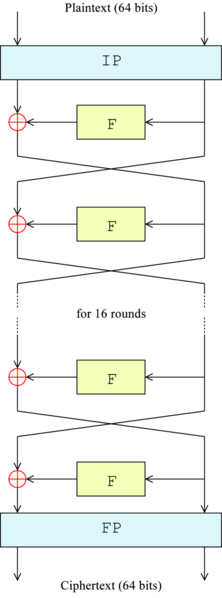
\includegraphics[scale=.7, angle=90]{informatika/algoritmy_a_ds/obrazky/DES-main-network.png}
      \caption{Struktura hlavní sítě algoritmu DES (zdroj: Wikipedie)}
    \end{center}
  \end{figure}

  \paragraph{Analýza:}
  \begin{pitemize}
    \item velká slabina je 64-bitový klíč (navíc efektivně pouze 56-bitový).
    Prolomen za méně než 24 hodin.
    \item úvodní permutace nemá prakticky žádný vliv
    \item existence slabých $(\mathbf{E}(K)=\mathbf{D}(K))$ a poloslabých
    $(\mathbf{E}(K_1)\mathbf{E}(K_2)=Id.)$ klíčů
    \item komplementárnost $C=\mathbf{E}(K,P)\Leftrightarrow\lnot C= \lnot
    \mathbf{E} (\lnot K,\lnot P)$
  \end{pitemize}
\end{obecne}

\begin{obecne}{Blowfish}
  \begin{pitemize}
    \item nástupce systému DES, 
    \item opět Feistelova šifra, délka bloku je 64 bitů, proměnná délka klíče až 448 bitů
    \item algoritmus provádí 16 cyklů nad vstupem délky 64-bitů
  \end{pitemize}
\end{obecne}

\begin{obecne}{IDEA}
  \begin{pitemize}
    \item z roku 1991, vyšel pod názvem IPES. 
    \item IDEA (International Data Encryption Algorithm)
    \item bloková šifra s délkou bloku 64-bitů a délkou klíče 128-bitu
    \item algoritmus je patentován 
    \item zajímavé je že pokud bychom algoritmus upravili tak, že bychom všechny řetězce
    se kterými pracuje zvětšili na dvojnásobek, tak dojde ke ztrátě bezpečnosti.
    \item algoritmus je považován za bezpečný.
  \end{pitemize}
\end{obecne}

\begin{obecne}{RC5}
  \begin{pitemize}
    \item z roku 1994 od R. Rivesta
    \item používá rotace závislé na datech.
    \item algoritmus umožňuje nastavit spoustu parametrů:
    \begin{pitemize}
      \item délka šifrovacího klíče (0\dots255 bytů)
      \item počet kol šifrovacího procesu (0\dots255)
      \item z hodnot 16, 32, 64, ale i vyšších lze zvolit délku slova, algoritmus
      zpracovává bloky o délce dvojnásobku slova
    \end{pitemize}
  \end{pitemize}

\end{obecne}

\begin{obecne}{Kryptosystém Rijndael}
  \begin{pitemize}
    \item produkční bloková šifra
    \item proměnná délka bloku~-- 16, 24 nebo 32 bajtů
    \item proměnná délka klíče~-- 128, 192 nebo 256 bitů
  \end{pitemize}

  \paragraph{Analýza:} Po rozsáhlé analýze nenalezena žádná slabina a tak
  zvolen jako nový standard AES.
\end{obecne}

\begin{obecne}{RC4}
  \begin{pitemize}
    \item proudová šifra od R. Rivesta
    \item jednoduchý a rychlý algoritmus 

    \paragraph{Analýza:} Zatím není známý žádný způsob útoku $\Rightarrow$
    algoritmus považován za bezpečný.
  \end{pitemize}
\end{obecne}

\begin{obecne}{FISH}
  \begin{pitemize}
    \item proudová šifra založena na Fibonacciho generátoru pseudonáhodných čísel.
    \item z fibonacciho generátoru se získá posloupnost a šifrovaní se provádí
    například XORováním této posloupnosti s \emph{P}
  \end{pitemize}
\end{obecne}

\begin{obecne}{Asymetrické}
  \begin{pitemize}
    \item šifry s asymetrickým klíčem~-- RSA, DSA (ElGammal)
    \item mnohem pomalejší
    \item není potřeba TTP
    \item pouze jeden klíč tajný, nemusí se měnit tak často
    \item o žádném schématu veřejného klíče nebylo dokázáno, že je bezpečné
  \end{pitemize}
\end{obecne}

\begin{obecne}{RSA}
  Kryptoschéma je založeno na Eulerově formuli: 
  $$a^{\varphi(n)} \equiv 1(mod\ n)$$ 
  kde $\varphi(n)$ je počet čísel z intervalu $1..n$ která jsou s $n$ nesoudělná.

  \paragraph{Šifrování:} Je třeba znát číslo $n$ a malé prvočíslo $e$. Otevřený
  text převedeme do posloupnosti modulo $n$. Každý blok $P_j$ zašifrujeme dle
  vzorce: $$C_j\equiv P_j^e\ (mod\ n)$$ Spojením výsledných bloků vznikne
  zašifrovaný text.

  \paragraph{Dešifrování:} Je třeba znát číslo $n$ a číslo $d$. Každý z bloků
  potom dešifrujeme takto: $$P_j\equiv C_j^d\ (mod\ n)$$ Pro dešifrovací klíč
  $d$ musí platit: $$ed\equiv 1\,(mod\ \varphi(n))$$ Prvočíslo $e$ nesmí dělit
  $\varphi(n)$. $d$ určíme z předchozího vztahu rozšířeným eukleidovým
  algoritmem.

  Veřejný klíč tvoří pár $(n, e)$, soukromý klíč pár $(n, d)$. Číslo $n$ musí být velmi
  velké a nesmí mít malé faktory. Pro reálné použití 100 až 200 bitů. Hranice bezpečnosti
  1024 bitů modulu $n$, rozumné 1500 bitů, lépe 2048 bitů.

  Není známa žádná metoda vedoucí k rozbití algoritmu RSA. 
\end{obecne}

\begin{obecne}{Merkle-Hellman kryptosystém}
  \begin{pitemize}
    \item založen na problému batohu
    \item plaintext je chápán jako posloupnost vah (řešení)
    \item ciphertext je výsledná hmotnost batohu
    \item pro superrostoucí posloupnost je problém řešitelný v lineárním čase
    \item superrostoucí posloupnost je součást soukromého klíče a tak
    dešifrování pomocí ní je zvládnutelné lineárně, kdežto bez ní je to NP-úplný
    problém
    \item systém byl prolomen! Není tedy považován za bezpečný. Útočník je
    schopen získat superrostoucí posloupnost a pomocí ní může dešifrovat
  \end{pitemize}
\end{obecne}

\begin{obecne}{Elgamal kryptosystém}
  Založen na obtížnosti výpočtu diskrétního logaritmu nad kruhem.

  Potřebujeme společný modul $q$ a číslo $g$ co nejvyššího řádu. Každý účastník si zvolí tajný
  klíč $y_i$ a vypočítá veřejný klíč $g^{y_i}$ mod $q$.
  \paragraph{Šifrování:} Nechť uživatel \emph{A} posílá zprávu \emph{P}
  uživateli \emph{B}. Náhodně
  vybere číslo $k$ a vypočítá: $$ g^k \mod q;\ P \otimes{(g^{y_b})}^k \mod q
  $$ obě čísla zašle \emph{B}.

  \paragraph{Dešifrování:} Uživatel \emph{B} vypočítá: $$ {(g^k)}^{y_b} \mod q$$
  a najde inverzní prvek. Z druhého čísla potom snadno získá \emph{P}.

  Systém je považován za bezpečný. Nevýhodou je nutnost generovat náhodné číslo
  $k$ a zdvojnásobení dat během šifrování.
\end{obecne}


\section{Sítě a internetové technologie}
\begin{pozadavky}
\begin{pitemize}
\item Architektura ISO/OSI
\item Rodina protokolu TCP/IP (ARP, IPv4, IPv6, ICMP, UDP, TCP) - adresace, routing, fragmentace, spolehlivost, flow control, congestion control, NAT
\item Rozhraní BSD sockets
\item Spolehlivost - spojované a nespojované protokoly, typy, detekce a oprava chyb
\item Bezpečnost - IPSec, principy fungování AH, ESP, transport mode, tunnel mode, firewalls
\item Internetové a intranetové protokoly a technologie - DNS, SMTP, FTP, HTTP, NFS, HTML, XML, XSLT a jejich použití.
\end{pitemize}
\end{pozadavky}
\subsection{Architektura ISO/OSI}

\subsubsection*{Úvod}
\begin{definice}
\textbf{Síťový model} je ucelená představa o tom, jak mají být sítě řešeny (obsahuje: počet vrstev, co má která vrstva na starosti; neobsahuje: konkrétní představu jak která vrstva plní své úkoly - tedy konkrétní protokoly). Příkladem je \emph{referenční model ISO/OSI} (konkrétní protokoly vznikaly samostatně a dodatečně).
\textbf{Síťová architektura} navíc obsahuje konkrétní protokoly - napr. \emph{rodina protokolů TCP/IP}.
\end{definice}

Referenčný model ISO/OSI (International Standards Organization / Open Systems Interconnection) bol pokusom vytvoriť univerzálnu sieťovú architektúru - ale skončil ako sieťový model (bez protokolov). Pochádza zo \uv{sveta spojov} - organizácie ISO, a bol \uv{oficiálnym riešením}, presadzovaným \uv{orgánmi štátu}; dnes už prakticky odpísaný - prehral v súboji s TCP/IP. ISO/OSI bol reakciou na vznik proprietárnych a uzavretých sietí. Pôvodne mal model popisovať chovanie otvorených systémov vo vnútri aj medzi sebou, ale bolo od toho upustené a nakoniec z modelu ostal len sieťový model (popis funkcionality vrstiev) a konkrétne protokoly pre RM ISO/OSI boli vyvíjané samostatne (a dodatočne zaraďované do rámca ISO/OSI).

Model vznikal maximalistickým spôsobom - obsahoval všetko čo by mohlo byť v budúcnosti potrebné. Vďaka rozsiahlosti štandardu sa implementovali len jeho niektoré podmnožiny - ktoré neboli (vždy) kompatibilné. Vznikol GOSIP (Government OSI Profile) určujúci podmnožinu modelu, ktorú malo mať implementované všetko štátne sieťové vybavenie. Naproti tomu všetkému TCP/IP vzniklo naopak - najprv navrhnutím jednoduchého riešenia, potom postupným obohacovaním o nové vlastnosti (tie boli zahrnuté až po preukázaní \uv{životaschopnosti}).

\subsubsection*{7 vrstev}
Kritériá pri návrhu vrstiev boli napr.: rovnomerná vyťaženosť vrstiev, čo najmenšie dátové toky medzi vrstvami, možnosť prevziať už existujúce štandardy (X.25), odlišné funkcie mali patriť do odlišných vrstiev, funkcie na rovnakom stupni abstrakcie mali patriť do rovnakej vrstvy. Niektoré vrstvy z finálneho návrhu sa používajú málo (relačná a prezentačná), niektoré zase príliš (linková - rozpadla sa na 2 podvrstvy LLC+MAC).

\begin{center}
\begin{tabular}{|c|l|}
	\hline
	aplikační vrstva & vrstvy orientované na podporu aplikací\\
	prezentační vrstva &\\
	relační vrstva &\\
	\hline
	transportní vrstva & přispůsobovací vrstva \\
	\hline
	síťová vrstva & vrstvy orientované na přenos dat\\
	linková vrstva & \\
	fyzická vrstva & \\
	\hline
\end{tabular}
\end{center}

\textbf{Fyzická vrstva} sa zaoberá prenosom bitov (kódovanie, modulácia, synchronizácia...) a ponúka teda služby typu pošli a príjmi bit (pričom neinterpretuje význam týchto dát). Pracuje sa tu s veličinami ako je \emph{šírka pásma}, \emph{modulačná a prenosová rýchlosť}.

\textbf{Linková vrstva} prenáša vždy celé bloky dát (rámce/frames), používa pritom fyzickú vrstvu a prenos vždy funguje len k priamym susedom. Môže pracovať spoľahlivo či nespoľahlivo, prípadne poskytovať QoS/best effort. Ďalej zabezpečuje riadenie toku - zaistenie toho, aby vysielajúci nezahltil príjemcu. Delí sa na dve podvrstvy - MAC (prístup k zdieľanému médiu - rieši konflikty pri viacnásobnom prístupe k médiu) a LLC (ostatné úlohy).  

\textbf{Sieťová vrstva} prenáša pakety (packets) - fakticky ich vkladá do linkových rámcov. Zaručuje doručenie paketov až ku konečnému adresátovi (tj. zabezpečuje smerovanie). Môže používať rôzne algoritmy smerovania - ne/adaptívne, izolované, distribuované, centralizované... (v architektúre TCP/IP je to IP vrstva)

\textbf{Transportná vrstva} zabezpečuje komunikáciu medzi koncovými účastníkmi (end-to-end) a môže meniť nespoľahlivý charakter komunikácie na spoľahlivý, menej spoľahlivý na viac spoľahlivý, nespojovaný prenos na spojovaný... Príkladom sú napr. TCP a UDP. Ďalšou úlohou je rozlišovanie jednotlivých entit (na rozdiel od napr. sieťovej vrstvy) v rámci uzlov - procesy, démony, úlohy (rozlišuje sa zväčša nepriamo - napr. v TCP/IP pomocou portov).

\textbf{Relačná vrstva} zaisťuje vedenie relácií - šifrovanie, synchronizáciu, podporu transakcií. Je to najkritizovanejšia vrstva v ISO/OSI modele, v TCP/IP úplne chýba.

\textbf{Prezentačná vrstva} slúži na konverziu dát, aby obe strany interpretovali dáta rovnako (napr. reálne čísla, rôzne kódovanie textov). Ďalej má na starosti konverziu dát do formátu, ktorý je možné preniesť: napr. linearizácia viacrozmerných polí, dátových štruktúr; konverzia viacbajtových položiek na jednotlivé byty (little vs. big endian). \emph{Poznámka}: Zápis čísla 1234H v Big endian je [12:34:--:--] (sun, motorola), v Little endian [--:--:34:12] (intel, amd, ethernet).

\textbf{Aplikačná vrstva} mala pôvodne obsahovať aplikácie - ale tých je veľa a nebolo možné ich štandardizovať. Teraz teda obsahuje len \uv{jadro} aplikácií - tie, ktoré malo zmysel štandardizovať (email a pod.). Ostatné časti aplikácií (GUI) boli vysunuté nad aplikačnú vrstvu.

\subsubsection*{Kritika}
Model ISO/OSI:
\begin{pitemize}
	\item je príliš zložitý, ťažkopádny a obtiažne implementovateľný
	\item je príliš maximalistický
	\item nerešpektuje požiadavky a realitu bežnej praxe
	\item počítal skôr s rozľahlými sieťami ako s lokálnymi
	\item niektoré činnosti (funkcie) zbytočne opakuje na každej vrstve
	\item jednoznačne uprednostňuje spoľahlivé a spojované prenosové služby (ale tie sú spojené s veľkou réžiou $\Rightarrow$ spoľahlivosť si efektívnejšie zabezpečia koncové uzly)
\end{pitemize}

Možnosť nespoľahlivého/nespojovaného spojenia bolo pridané do štandardu až dodatočne, napriek tomu bol porazený architektúrou TCP/IP. Používajú sa však niektoré prevzaté prokoly - X.400 (elektronická pošta), X.500 (adresárové služby - odľahčením vznikol úspešný protokol LDAP).

\subsection{Rodina protokolů TCP/IP (ARP, IPv4, IPv6, ICMP, UDP, TCP) -- adresace, routing, fragmentace, spolehlivost, flow control, congestion control, NAT}
\begin{center}
\begin{tabular}{|c|c|}
	\hline
	ISO/OSI & TCP/IP \\
	\hline
	\hline
	aplikační vrstva & aplikační vrstva\\
	prezentační vrstva &\\
	relační vrstva &\\
	\hline
	transportní vrstva & transportní vrstva \\
	\hline
	síťová vrstva & síťová vrstva (též IP vrstva) \\
	\hline
	linková vrstva & vrstva síťového rozhraní\\
	fyzická vrstva & \\
	\hline
\end{tabular}
\end{center}

Obvyklé označenie je \emph{TCP/IP protocol suite} (súčasťou je viac ako 100 protokolov). Architektúra vznikla postupne (v akademickom prostredí, neskôr sa rozšírila aj do komerčnej sféry) -- najprv vznikli protokoly, potom vrstvy -- a od vzniku sa toho zmenilo len málo (zmeny sú aditívne). Je to najpoužívanejšia sieťová technológia (IP over everything, everything over IP). Prístup autorov bol, na rozdiel od ISO/OSI, od jednoduchšieho k zložitejšiemu -- najprv sa vytvárajú jednoduché riešenia, ktoré sa postupne obohacujú. Až sa riešenie prakticky overí (2 nezávislé implementácie), vznikne štandard. TCP/IP predpokladá že siete sú typu nespojované, nespoľahlivé a best effort. Všetká inteligencia je sústredená do koncových uzlov, sieť je \uv{hlúpa} ale rýchla.

TCP/IP bol pôvodne určený pre ARPAnet -- nemohol mať teda žiadnu centrálnu časť a musel byť robustný voči chybám (nespoľahlivé/nespojované prenosy). Dôraz sa kládol aj na "internetworking". Nebolo však požadované zabezpečenie, mobilita ani kvalita služieb.

TCP/IP nedefinuje rôzne siete (čo sa hardvérových vlastností týka) a technológie vo vrstve sieťového rozhrania -- iba sa snaží nad nimi prevádzkovať protokol IP (okrem SLIP a PPP pre dvojbodové spoje). V sieťovej vrstve je IP protokol, v transportnej jednotné transportné protokoly (TCP a UDP), v aplikačnej potom jednotné základy aplikácií (email, prenos súborov, remote login...).

\subsubsection*{Adresace, IPv4, IPv6}
Data se v IP síti posílají po blocích nazývaných datagramy. Jednotlivé datagramy putují sítí zcela nezávisle, na začátku komunikace není potřeba navazovat spojení či jinak \uv{připravovat cestu} datům, přestože spolu třeba příslušné stroje nikdy předtím nekomunikovaly.

IP protokol v doručování datagramů poskytuje nespolehlivou službu, označuje se také jako best effort – \uv{nejlepší úsilí}; tj. všechny stroje na trase se datagram snaží podle svých možností poslat blíže k cíli, ale nezaručují prakticky nic. Datagram vůbec nemusí dorazit, může být naopak doručen několikrát a neručí se ani za pořadí doručených paketů. Pokud aplikace potřebuje spolehlivost, je potřeba ji implementovat v jiné vrstvě síťové architektury, typicky protokoly bezprostředně nad IP (viz TCP).

Pokud by síť často ztrácela pakety, měnila jejich pořadí nebo je poškozovala, výkon sítě pozorovaný uživatelem by byl malý. Na druhou stranu příležitostná chyba nemívá pozorovatelný efekt, navíc se obvykle používá vyšší vrstva, která ji automaticky opraví.

V \textbf{IPv4} je \emph{adresou} 32bitové číslo, zapisované po jednotlivých bajtech, oddělených tečkami. Takových čísel existuje celkem $2^{32}$. Určitá část adres je ovšem rezervována pro vnitřní potřeby protokolu a nemohou být přiděleny. Dále pak praktické důvody vedou k tomu, že adresy je nutno přidělovat hierarchicky, takže celý adresní prostor není možné využít beze zbytku. To vede k tomu, že v současnosti je již znatelný nedostatek IP adres, který řeší různými způsoby: dynamickým přidělováním (tzn. např. každý uživatel dial-up připojení dostane dočasnou IP adresu ve chvíli, kdy se připojí, ale jakmile se odpojí, je jeho IP adresa přidělena někomu jinému; při příštím připojení pak může tentýž uživatel dostat úplně jinou adresu), překladem adres (NAT) a podobně. Ke správě tohoto přidělování slouží specializované síťové protokoly, jako např. DHCP.

Pôvodný koncept adries počítal so štruktúrou adresy IPv4 v tvare \emph{sieť:počítač}, kde bolo delenie častí pevne dané. Neskôr sa to ale ukázalo ako príliš hrubé delenie a lokálna časť adresy (v rámci jednej podsiete) može mäť dnes promenlivú dĺžku. Obecne platí, že medzi adresami v rovnakej podsieti (majú rovnakú sieťovú časť) je možné dopravovať dáta priamo -- dotyční účastníci sú prepojení jedným ethernetom alebo inou lokálnou sieťou. V opačnom prípade sa dáta dopravujú \emph{smerovačmi/routermi}. Hranicu v adrese medzi adresou siete a počítača určuje dnes maska podsiete. Jedná sa o 32 bitovú hodnotu, ktorá obsahuje jednotky tam, kde je v adrese určená sieť.

\textbf{Adresovanie sietí} bolo v prvopočiatkoch internetu vyriešené staticky -- prvých 8 bitov adresy určovalo sieť, zvyšok jednotlivé počítače (existovať tak mohlo max. 256 sietí). S nástupom lokálnych sietí bolo tento systém potrebné zmeniť -- zaviedli sa \emph{triedy IP adries}. Existovalo 5 tried (A(začiatok 0, hodnoty prvého bajtu 0-127, maska 255.0.0.0), B(10, 128-191, 255.255.0.0), C(110, 192-223, 255.255.255.0), D(1110, 224-239, určené na multicast) a E(1111, 240-255, určené ako rezerva)). Postupom času sa ale aj toto rozdelenie ukázalo ako nepružné a bol zavedený CIDR (Classless Inter-Domain Routing) systém v ktorom je možné hranicu medzi adresou siete a lokálnou časťou adresy umiestniť ľubovoľne (označuje sa potom ako kombinácia prefixu a dĺžky vo forme 192.168.0.0/24, kde 24 znamená že adresu tvorí prvých 24 bitov -- jiný zápis je pomocí už zmiňované masky podsítě, tj. 192.168.0.0 s maskou 255.255.255.0).

Medzi adresami existujú niektoré tzv. \textbf{vyhradené adresy}, ktoré majú špeciálny význam.
\begin{pitemize}
	\item Adresa s (binárnymi) nulami v časti určujúcej počítač (192.168.0.\textbf{0} (/24)) znamená \uv{táto sieť}, resp. \uv{táto stanica}.
	\item Adresa s jednotkami v časti určujúcej počítač (192.168.0.\textbf{255} (/24)) znamená broadcast -- všesmerové vysielanie.
	\item Adresy 10.0.0.0 -- 10.255.255.255, 172.16.0.0 -- 172.31.255.255 a 192.168.0.0 -- 192.168.255.255 sa používajú na adresovanie interných sietí -- smerovače tieto adresy nesmie smerovať ďalej do internetu.
\end{pitemize}

\textbf{IPv6} je trvalejším riešením nedostatku adries -- zatiaľ sa ale rozširuje veľmi pozvolna. Adresa v IPv6 má dĺžku 128 bitov (oproti 32), čo znamená cca. $6 \times 10^{23}$ IP adries na $1 m^2$ zemského povrchu -- umožňuje teda, aby každé zariadenie na zemi malo vlastnú jednoznačnú adresu. Adresa IPv6 sa zapisuje ako osem skupín po štyroch hexadecimálnych číslach (napr. 2001:0718:1c01:0016:0214:22ff:fec9:0ca5) -- pričom úvodné nuly v číslach je možné vynechať. Ak po sebe nasleduje niekoľko nulových skupín, je možné použiť len znaky :: -- napr. ::1 miesto 0000:0000:.......:0001. Toto je možné použiť len raz v zápise adresy. RFC 4291 zavádza 3 typy adries:
\begin{pitemize}
	\item \textbf{inidividuálne / unicast} -- identifikujú práve jedno rozhranie
	\item \textbf{skupinové / multicast} -- určuje skupinu zariadení, ktorým sa má správa dopraviť
	\item \textbf{výberové / anycast} -- určuje tiež skupinu zariadení, dáta sa však doručia len jednému z členov (najbližšiemu)
\end{pitemize}
IPv6 neobsahuje všesměrové (broadcast) adresy. Byly nahrazeny obecnějším modelem skupinových adres a pro potřeby doručení dat všem zařízením připojeným k určité síti slouží speciální skupinové adresy (např. ff02::1 označuje všechny uzly na dané lince).

IPv6 zavádí také koncepci dosahu (scope) adres. Adresa je jednoznačná vždy jen v rámci svého dosahu. Nejčastější dosah je pochopitelně globální, kdy adresa je jednoznačná v celém Internetu. Kromě toho se často používá dosah linkový, definující jednoznačnou adresu v rámci jedné linky (lokální sítě, např. Ethernetu). Propracovanou strukturu dosahů mají skupinové adresy (viz níže).

Adresní prostor je rozdělen následovně:
\begin{center}
\begin{tabular}{|l|l|}
	\hline
	prefix & význam \\
	\hline
	\hline
	::/128 & neurčená \\
	::1/128 & smyčka (loopback) \\
	ff00::/8 & skupinové \\
	fe80::/10 & individuální lokální linkové \\
	ostatní & individuální globální \\
	\hline
\end{tabular}
\end{center}

Výběrové adresy nemají rezervovánu svou vlastní část adresního prostoru. Jsou promíchány s individuálními a je otázkou lokální konfigurace, aby uzel poznal, zda se jedná o individuální či výběrovou adresu.

Strukturu globálních individuálních IPv6 adres definuje RFC 3587. Je velmi jednoduchá a de facto odpovídá (až na rozměry jednotlivých částí) výše uvedené struktuře IPv4 adresy.

\begin{center}
\begin{tabular}{|l|l|l|}
	\hline
	n bitů & 64-n bitů & 64 bitů \\
	globální směrovací prefix & adresa podsítě & adresa rozhraní \\
	\hline
\end{tabular}
\end{center}

Globální směrovací prefix je de facto totéž co adresa sítě, následuje adresa podsítě a počítače (přesněji síťového rozhraní). V praxi je adresa podsítě až na výjimky 16bitová a globální prefix 48bitový. Ten je pak přidělován obvyklou hierarchií, jejíž stávající pravidla jsou:
\begin{pitemize}
    \item první dva bajty obsahují hodnotu 2001 (psáno v šestnáctkové soustavě)
    \item další dva bajty přiděluje regionální registrátor (RIR)
    \item další dva bajty přiděluje lokální registrátor (LIR)
\end{pitemize}

Reálná struktura globální individuální adresy tedy vypadá následovně:

\begin{center}
\begin{tabular}{|l|l|l|l|l|}
	\hline
	16 bitů & 16 bitů & 16 bitů & 16 bitů & 64 bitů \\
	2001 & přiděluje RIR &přiděluje LIR &adresa podsítě & adresa rozhraní \\
	\hline
\end{tabular}
\end{center}
Adresa rozhraní by pak měla obsahovat modifikovaný EUI-64 identifikátor. Ten získáte z MAC adresy jednoduchým postupem: invertuje se druhý bit MAC adresy a doprostřed se vloží dva bajty obsahující hodnotu fffe. Z ethernetové adresy 00:14:22:c9:0c:a5 tak vznikne identifikátor 0214:22ff:fec9:0ca5.

Adresy začínajúce hodnotou ff sú tzv. "skupinové adresy" -- štyri nasledujúce bity v nej obsahujú príznaky, ďalšie štyri potom dosah (napr. interface-local, link-local, admin-local, site-local, organization-local, global...)

IPv6 ďalej podporuje QoS a bezpečnosť (IPsec).

\subsubsection*{Routing} 
Pojmem \textbf{směrování} (routing, routování) je označováno hledání cest v počítačových sítích. Jeho úkolem je dopravit datový paket určenému adresátovi, pokud možno co nejefektivnější cestou. Síťová infrastruktura mezi odesílatelem a adresátem paketu může být velmi složitá. Směrování se proto zpravidla nezabývá celou cestou paketu, ale řeší vždy jen jeden krok – komu data předat jako dalšímu (tzv. \uv{distribuované směrování}). Ten pak rozhoduje, co s paketem udělat dál.

V prípade, že je cieľová stanica packetu v rovnakej sieti ako je odosielateľ, o doručenie sa postará linková vrstva. V opačnom prípade musí odosielateľ určiť najvhodnejší odchodzí smer a poslať datagram smerovaču vo zvolenom smere.

Základní datovou strukturou pro směrování je směrovací tabulka (routing table). Představuje vlastně onu sadu ukazatelů, podle kterých se rozhoduje, co udělat s kterým paketem. Směrovací tabulka je složena ze záznamů obsahujících:
\begin{pitemize}
	\item cílovou adresu, které se dotyčný záznam týká. Může se jednat o adresu individuálního počítače, častěji však je cíl definován prefixem, tedy začátkem adresy. Prefix mívá podobu 147.230.0.0/16. Hodnota před lomítkem je adresa cíle, hodnota za lomítkem pak určuje počet významných bitů adresy. Uvedenému prefixu tedy vyhovuje každá adresa, která má v počátečních 16 bitech (čili prvních dvou bajtech) hodnotu 147.230.
    \item akci určující, co provést s datagramy, jejichž adresa vyhovuje prefixu. Akce mohou být dvou typů: doručit přímo adresátovi (pokud je dotyčný stroj s adresátem přímo spojen) nebo předat některému ze sousedů (jestliže je adresát vzdálen).
\end{pitemize}

Směrovací rozhodnutí pak probíhá samostatně pro každý procházející datagram. Vezme se jeho cílová adresa a porovná se směrovací tabulkou následovně:
\begin{pitemize}
	\item Z tabulky se vyberou všechny vyhovující záznamy (jejichž prefix vyhovuje cílové adrese datagramu).
	\item Z vybraných záznamů se použije ten s nejdelším prefixem. Toto pravidlo vyjadřuje přirozený princip, že konkrétnější záznamy (jejichž prefix je delší, tedy přesnější; specielním případem je \emph{host-specific route}) mají přednost před obecnějšími (co může být např. i \emph{default route}; ps: \emph{agregace}).
\end{pitemize}

Zajímavou otázkou je, jak vznikne a jak je udržována směrovací tabulka. Tento proces mají obecně na starosti směrovací algoritmy. Když jsou pak pro určitý algoritmus definována přesná pravidla komunikace a formáty zpráv nesoucích směrovací informace, vznikne směrovací protokol (routing protocol). Směrovací algoritmy můžeme rozdělit do dvou základních skupin: na statické a dynamické. Často se také mluví o statickém a dynamickém směrování, které je důsledkem činnosti příslušných protokolů.

Při \textbf{statickém (též neadaptivním) směrování} se směrovací tabulka nijak nemění. Je dána konfigurací počítače a případné změny je třeba v ní provést ručně. Tato varianta vypadá jako nepříliš atraktivní, ve skutečnosti ale drtivá většina zařízení v Internetu směruje staticky.

\textbf{Dynamické (adaptivní) směrování} průběžně reaguje na změny v síťové topologii a přizpůsobuje jim směrovací tabulky. Na vytváranie tabuliek existuje niekoľko algoritmov -- routovacích protokolov (vector-distance/link-state) -- RIP, BGP, OSPF.

\medskip
\begin{obecne}{Distribuované směrování}
V distribuovaném směrování může výpočet cesty (směru předání paketu) provádět buď každý uzel nezávisle, nebo mohou uzly kooperovat (distribuovaný výpočet). Rozlišuje se také četnost aktualizace informací. Dva základní algoritmy distribuovaného směrování jsou:
\begin{pitemize}
    \item \emph{vector distance} -- každý uzel si udržuje tabulku vzdáleností, přímí sousedé si vyměňují informace o cestách ke všem uzlům, tj. jde o distribuovaný výpočet, přenáší se dost informací. Trpí problémem \uv{count-to-infinity} -- tj. když 1 uzel přestane existovat, postupně si jeho sousedé mezi sebou přehazují vzdálenost, postupně o 1 zvětšovanou (do nekonečna). Řeší se pomocí technik \uv{split horizon} (neinzeruj vzdálenost zpět) a \uv{poisoned reverse} (inzeruj zpět nekonečno), někde ale přesto selhává.
    \item \emph{link state} -- každý uzel hledá změny svých sousedů a pokud k nějaké dojde, pošle floodem informaci do celé sítě. Výpočet vzdáleností dělá každý uzel sám.
\end{pitemize}
Tyto algoritmy se používají u některých známých směrovacích protokolů:
\begin{pitemize}
    \item \emph{RIP} (Routing Information Protocol) -- protokol z BSD Unixu, typu vector distance. Počítá s max. 16 přeskoky, změny se updatují 2x za minutu. Informace ve směrovací tabulce může zahrnovat max. 25 sítí, používá split horizon \& poisoned reverse. Hodí se ale jen pro malé sítě.
    \item \emph{OSPF} (Open Shortest Path First) -- jde o protokol typu link state, uzly si počítají vzdálenosti do všech sítí Dijkstrovým algoritmem. Pro zjišťování změn se posílají pakety "HELLO" a "ECHO". Má lepší škálovatelnost, hodí se pro větší sítě.
\end{pitemize}
\end{obecne}

\begin{obecne}{Hierarchické směrování, autonomní systémy}
Hierarchické směrování znamená rozdělení sítě do oblastí (\emph{areas}) a směrování mezi nimi jen přes vstupní body. Je vhodné pro velké, složitě propojené nebo různým způsobem spravované sítě. Nad oblastmi se vytvoří propojení -- \emph{backbone area} (páteřní systém), přes které se směrování mezi oblastmi provádí. Celému tomuto (areas + backbone area) se říká \emph{autonomní systém}. Detailní směrovací informace neopouštějí jednotlivé oblasti. 

Pro směrování v rámci jedné oblasti i mezi oblastmi v rámci jednoho autonomního systému slouží jeden z tzv. \emph{interior gateway protocol}s, může být použit např. OSPF nebo RIP, případně další jako IGRP (interior gateway routing protocol, typu vector distance) nebo EIGRP (enhaced IGRP, hybrid mezi vector distance a link state). Mezi jednotlivými autonomními systémy (přes AS boundary routers) se směruje pomocí \emph{exterior gateway protocolu}, jedním z nich je např. \emph{Border Gateway Protocol} (BGP).

Díky existenci autonomních systémů jde např. při peeringu stanovit, který provoz půjde přes peering a který výše po upstreamu do páteřních sítí.
\end{obecne}


\subsubsection*{Fragmentace}

\textbf{Maximum transmission unit} (MTU) je maximální velikost paketu, který je možné přenést z jednoho síťového zařízení na druhé. Obvyklá hodnota MTU v případě Ethernetu je cca 1500 bajtů, nicméně mezi některými místy počítačové sítě (spojených například modemem nebo sériovou linkou) může být maximální délka přeneseného paketu nižší. Hodnotu MTU lze zjistit prostřednictvím protokolu ICMP. Při posílání paketů přes několik síťových zařízení je samozřejmě důležité nalézt nejmenší MTU na dané cestě. Hodnota MTU je omezena zdola na 576 bajtů.

U přenosového protokolu TCP je při směrování paketu do přenosového kanálu s nižším MTU než je délka paketu, provedena \textbf{fragmentace paketu}. U protokolu UDP není fragmentace paketu podporována a paket je v takovém případě zahozen.

 Pokud dorazí na směrovač paket o velikosti větší, než kterou je přenosová trasa schopna přenést (např. při přechodu z Token Ringu používajícího 4 kByte pakety na Ethernet používajícího maximálně 1,5 kByte pakety), musí směrovač zajistit tzv. fragmentaci, neboli rozebrání paketu na menší části a cílový uzel musí zajistit opětovné složení, neboli defragmentaci.

Fragmenty procházejí přes síť jako samostatné datagramy. Aby byl koncový uzel schopen fragmenty složit do originálního datagramu, musí být fragmenty příslušně označeny. Toto označování se provádí v příslušných polích IP hlavičky.

Pokud nesmí být datagram fragmentován, je označen v příslušném místě IP hlavičky příznakem \uv{Don`t Fragment}. Jestliže takto označený paket dorazí na směrovač, který by jej měl poslat prostředím s nižším MTU a tudíž je nutnost provést fragmentaci, provede směrovač jeho zrušení a informuje odesílatele chybovou zprávou ICMP. 

Aby byl cílový uzel schopen složit originální datagram, musí mít dostatečný buffer do něhož jsou jednotlivé fragmenty ukládány na příslušnou pozici danou offsetem. Složení je dokončeno v okamžiku, kdy je vyplněn celý datagram začínající fragmentem s nulovým offsetem (identification a fragmentation offset v hlavičke) a končící segmentem s příznakem \uv{More Data Flag} (resp. More Fragments) nastaveným na False.

V IPv4 je možné fragmentované pakety ďalej deliť; naproti tomu v IPv6 musí fragmentáciu zabezpečiť odosielateľ -- nevyhovujúce pakety sa zahadzujú.


\subsubsection*{Spolehlivost, Flow control, Congestion control}
Keďže TCP/IP funguje nad obecne nespojovanými a nespoľahlivými médiami, \textbf{spoľahlivosť} ktorú TCP poskytuje nie je \uv{skutočná}, ale len \uv{softvérovo emulovaná} -- medziľahlé uzly o spojení nič nevedia, fungujú nespojovane (pre komunikáciu sa používa sieťová vrstva, transportná \uv{existuje} iba medzi koncovými uzlami). Je teda nutné ošetriť napr. nespoľahlivosť infraštruktúry (strácanie dát, duplicity -- pričom stratiť sa môže aj žiadosť o vytvorenie pripojenia, potvrdenie...) a reboot uzlov (uzol stratí históriu, je potrebné ošetriť existujúce spojenia...).

Používa sa celá rada techník, kde základom je kontinuálne potvrdzovanie: príjemca posiela kladné potvrdenia; odosielateľ po každom odoslaní spúšťa časovač a ak mu do vypršania nepríde potvrdenie, posiela dáta znovu.  Potvrdzovanie nie je samostatné ale vkladá sa do paketov cestujúcich opačným smerom -- \emph{piggybacking}.

TCP priebežne kontroluje \uv{dobu obrátky} a vyhodnocuje vážený priemer a rozptyl dôb obrátky. Čakaciu dobu (na potvrdenie) potom vypočítava ako funkciu tohto váženého priemeru a rozptylu. Výsledný efekt je potom ten, že čakacia doba je tesne nad strednou dobou obrátky. V prípade konštantnej doby obrátky sa čakacia doba približuje strednej dobe obrátky; ak kolíše, čakacia doba sa zväčšuje.

Dáta v TCP sa príjímajú/posielajú po jednotlivých byteoch -- interne sa však bufferujú a posielajú až po naplnení buffera (pričom aplikácia si môže vyžiadať okamžité odoslanie -- operácia PUSH). TCP si potrebuje označovať jednotlivé byty v rámci prúdu (keďže nepracuje s blokmi) -- napr. kvôli potvrdzovaniu; používa sa na to 32-bitová pozícia v bytovom prúde (začína sa od náhodne zvoleného čísla).

TCP sa snaží \textbf{riadiť tok dát} -- aby odosielateľ nezahlcoval príjemcu a kvôli tomu nedochádzalo k stráte dát. Podstata riešenia je tzv. \emph{metóda okienka}. Okienko udáva veľkosť voľných bufferov na strane prijímajúceho a odosielateľ môže posielať dáta až do \uv{zaplnenia} okienka. Príjemca spolu s každým potvrdením posiela aj svoju ponuku -- údaj o veľkosti okienka (window advertisment)., ktorý hovorí koľko ešte dát je schopný prijať (naviac k práve potvrdeným). Znovu -- používa sa metóda kontinuálneho potvrďovania.

Väčšina strát prenášaných dát ide skôr na vrub zahlteniu ako chybám HW a transportné protokoly môžu nevhodným chovaním zhoršovať dôsledky. TCP každú stratu dát chápe ako dôsledok zahltenia -- nasadzuje \textbf{opatrenia proti zahlteniu} (congestion control). Po stráte paketu ho pošle znovu ale neposiela ďalšie a čaká na potvrdenie (tj. prechod z kontinuálneho potvrdzovania na jednotlivé $\Rightarrow$ vysiela menej dát ako mu umožňuje okienko). Ak príde potvrdenie včas, zdvojnásobí množstvo odosielaných dát -- a tak pokračuje kým nenarazí na aktuálnu veľkosti okienka (postupne sa tak vracia na kontinuálne potvrdzovanie).

Dôležitou vlastnosťou je aj korektné chovanie pri naväzovaní a rušení spojenia (v prostredí, kde môže dôjsť k spomaleniu, strate, duplicite...) -- používa sa tzv. 3-fázový handshake. Vytvorenie spojenia prebieha nasledovne:
\begin{enumerate}
	\item Klient pošle serveru SYN paket (v pakete je nastavený príznak SYN) spolu s náhodným \emph{sequence number} (X).
	\item Server tento paket prijme, zaznamená si sequence number (X) a pošle späť paket SYN-ACK. Tento paket obsahuje pole Acknowledgement, ktoré označuje ďalšie číslo (sequence number), ktoré tento host očakáva (X+1). Tento host rovno vytvorí spätnú session s vlastným sekvenčným číslom (Y).
	\item Klient odpovie so sekvenčným číslom (X+1) a jednoduchým Acknowledgement číslom (Y+1) -- čo je sekvenčné číslo servera+1.
\end{enumerate}
Pak už spojení považováno za navázané. Rušenie spojenia funguje podobne, posílají se pakety FIN (finish), FIN+ACK a ACK. Pokud více než nějaký určitý počet pokusů o odeslání (po spočítaných time-outech) jednoho z 3-way handshake paketů selže (druhá strana neodešle to, co mělo následovat), spojení se považuje za přerušené (i u navazování, i u rušení).

\subsubsection*{NAT}

TODO: přeložit ty copy \& paste z Wiki

Network address translation (zkráceně NAT, česky překlad síťových adres) je funkce síťového routeru pro změnu IP adres packetů procházejících zařízením, kdy se zdrojová nebo cílová IP adresa převádí mezi různými rozsahy. Nejběžnější formou je tzv. maškaráda (maskování), kdy router IP adresy z nějakého rozsahu mění na svoji IP adresu a naopak -- tím umožňuje, aby počítače ve vnitřní síti (LAN) vystupovaly v Internetu pod jedinou IP adresou. Router si drží po celou dobu spojení v paměti tabulku překladu adres.

Překlad síťových adres je funkce, která umožňuje překládání adres. Což znamená, že adresy z lokální sítě přeloží na jedinečnou adresu, která slouží pro vstup do jiné sítě (např. Internetu), adresu překládanou si uloží do tabulky pod náhodným portem, při odpovědi si v tabulce vyhledá port a pošle pakety na IP adresu přiřazenou k danému portu. NAT je vlastně jednoduchým proxy serverem (na sieťovej vrstve).

\medskip
\begin{obecne}{Komunikace}
Klient odešle požadavek na komunikace, směrovač se podívá do tabulky a zjistí, zdali se jedná o adresu lokální, nebo adresu venkovní. V případě venkovní adresy si do tabulky uloží číslo náhodného portu, pod kterým bude vysílat a k němu si přiřadí IP adresu. Během přeposílání \uv{ven} a změny adresy v paketu musí NAT také přepočítat CRC checksum TCP i IP (aby pakety nebyly zahazovány kvůli špatnému CRC, protože změněná adresa je jejich součástí).

Výhodami NAT sú umožnenie pripojenie viacerých počítačov do internetu cez jednu zdieľanú verejnú IP adresu, a zvýšenie bezpečnosti počítačov za NATom (aj keď je to security through obscurity a nie je dobré postaviť bezpečnosť iba na NATe). Nevýhodami potom sú nefungujúce protokoly (napr. aktívne FTP) -- čo je zrejmé z fungovania NATu.
\end{obecne}

\begin{obecne}{NAT Traversal}
NAT traversal refers to an algorithm for the common problem in TCP/IP networking of establishing connections between hosts in private TCP/IP networks that use NAT devices.

This problem is typically faced by developers of client-to-client networking applications, especially in peer-to-peer and VoIP activities. NAT-T is commonly used by IPsec VPN clients in order to have ESP packets go through NAT.

Many techniques exist, but no technique works in every situation since NAT behavior is not standardized. Many techniques require a public server on a well-known globally-reachable IP address. Some methods use the server only when establishing the connection (such as STUN), while others are based on relaying all the data through it (such as TURN), which adds bandwidth costs and increases latency, detrimental to conversational VoIP applications.
\end{obecne}

\begin{obecne}{Druhy uspořádání NATu}
\begin{pitemize}
\item \emph{Static NAT}: A type of NAT in which a private IP address is mapped to a public IP address, where the public address is always the same IP address (i.e., it has a static address). This allows an internal host, such as a Web server, to have an unregistered (private) IP address and still be reachable over the Internet.

\item \emph{Dynamic NAT}--- A type of NAT in which a private IP address is mapped to a public IP address drawing from a pool of registered (public) IP addresses. Typically, the NAT router in a network will keep a table of registered IP addresses, and when a private IP address requests access to the Internet, the router chooses an IP address from the table that is not at the time being used by another private IP address. Dynamic NAT helps to secure a network as it masks the internal configuration of a private network and makes it difficult for someone outside the network to monitor individual usage patterns. Another advantage of dynamic NAT is that it allows a private network to use private IP addresses that are invalid on the Internet but useful as internal addresses.

\item \emph{PAT} --- PAT (NAT overloading) je další variantou NATu. U této varianty NATu se více inside local adres mapuje na jednu inside global adresu na různých portech. Tedy máme jednu veřejnou adresu a vnitřní síť oadresovanou inside local adresami. 
Překladová tabulka je rozšířena o dvě položky: inside local port -- port, ze kterého byl paket odeslán a inside global port -- číslo portu, na který je paket odeslaný ze zdrojového portu počítače mapován. Výhodou je, že se tak připojuje více počítačů přes jednu IP adresu.
\end{pitemize}
\end{obecne}


\subsubsection*{ARP}

\textbf{Address Resolution Protocol (ARP)} se v počítačových sítích s IP protokolem používá k získání ethernetové (MAC) adresy sousedního stroje z jeho IP adresy. Používá se v situaci, kdy je třeba odeslat IP datagram na adresu ležící ve stejné podsíti jako odesílatel. Data se tedy mají poslat přímo adresátovi, u něhož však odesílatel zná pouze IP adresu. Pro odeslání prostřednictvím např. Ethernetu ale potřebuje znát cílovou ethernetovou adresu.

Proto vysílající odešle ARP dotaz (ARP request) obsahující hledanou IP adresu a údaje o sobě (vlastní IP adresu a MAC adresu). Tento dotaz se posílá linkovým broadcastem – na MAC adresu identifikující všechny účastníky dané lokální sítě (v případě Ethernetu na ff:ff:ff:ff:ff:ff). ARP dotaz nepřekročí hranice dané podsítě, ale všechna k ní připojená zařízení dotaz obdrží a jako optimalizační krok si zapíší údaje o jeho odesílateli (IP adresu a odpovídající MAC adresu) do své ARP cache. Vlastník hledané IP adresy pak odešle tazateli ARP odpověď (ARP reply) obsahující vlastní IP adresu a MAC adresu. Tu si tazatel zapíše do ARP cache a může odeslat datagram.

Informace o MAC adresách odpovídajících jednotlivým IP adresám se ukládají do ARP cache, kde jsou uloženy do vypršení své platnosti. Není tedy třeba hledat MAC adresu před odesláním každého datagramu – jednou získaná informace se využívá opakovaně. V řadě operačních systémů (Linux, Windows XP) lze obsah ARP cache zobrazit a ovlivňovat příkazem arp.

Alternativou pro počítač bez ARP protokolu je používat tabulku přiřazení MAC adres IP adresám definovanou jiným způsobem, například pevně konfigurovanou. Tento přístup se používá především v prostředí se zvýšenými nároky na bezpečnost, protože v ARP se dá podvádět – místo skutečného vlastníka hledané IP adresy může odpovědět někdo jiný a stáhnout tak k sobě jeho data.

ARP je definováno v RFC 826. Používá se pouze pro IPv4. Novější verze IP protokolu (IPv6) používá podobný mechanismus nazvaný Neighbor Discovery Protocol (NDP, \uv{objevování sousedů}).

Ačkoliv se ARP v praxi používá téměř výhradně pro překlad IP adres na MAC adresy, nebyl původně vytvořen pouze pro IP sítě. ARP se může použít pro překlad MAC adres mnoha různých protokolů na síťové vrstvě. ARP byl také uzpůsoben tak, aby vyhodnocoval jiné typy adres fyzické vrstvy: například ATMARP se používá k vyhodnocení ATM NSAP adres v protokolu Classical IP over ATM.

\subsubsection*{ICMP}

\textbf{ICMP protokol (anglicky Internet Control Message Protocol)} je jeden z jádrových protokolů ze sady protokolů internetu. Používají ho operační systémy počítačů v síti pro odesílání chybových zpráv -- například pro oznámení, že požadovaná služba není dostupná nebo že potřebný počítač nebo router není dosažitelný.

ICMP se svým účelem liší od TCP a UDP protokolů tím, že se obvykle nepoužívá sítovými aplikacemi přímo. Jedinou výjimkou je nástroj ping, který posílá ICMP zprávy \uv{Echo Request} (a očekává příjem zprávy \uv{Echo Response}) aby určil, zda je cílový počítač dosažitelný a jak dlouho paketům trvá, než se dostanou k cíli a zpět.

ICMP protokol je součást sady protokolů internetu definovaná v RFC 792. ICMP zprávy se typicky generují při chybách v IP datagramech (specifikováno v RFC 1122) nebo pro diagnostické nebo routovací účely. Verze ICMP pro IPv4 je známá jako ICMPv4. IPv6 používá obdobný protokol: ICMPv6.

ICMP zprávy se konstruují nad IP vrstvou; obvykle z IP datagramu, který ICMP reakci vyvolal. IP vrstva patřičnou ICMP zprávu zapouzdří novou IP hlavičkou (aby se ICMP zpráva dostala zpět k původnímu odesílateli) a obvyklým způsobem vzniklý datagram odešle. Například každý stroj (jako třeba mezilehlé routery), který forwarduje IP datagram, musí v IP hlavičce dekrementovat políčko TTL (\uv{time to live}, \uv{zbývající doba života}) o jedničku. Jestliže TTL klesne na 0 (a datagram není určen stroji provádějícímu dekrementaci), router přijatý paket zahodí a původnímu odesílateli datagramu pošle ICMP zprávu \uv{Time to live exceeded in transit} (\uv{během přenosu vypršela doba života}).

Každá ICMP zpráva je zapouzdřená přímo v jediném IP datagramu, a tak (jako u UDP) ICMP nezaručuje doručení. Ačkoli ICMP zprávy jsou obsažené ve standardních IP datagramech, ICMP zprávy se zpracovávají odlišně od normálního zpracování prokolů nad IP. V mnoha případech je nutné prozkoumat obsah ICMP zprávy a doručit patřičnou chybovou zprávu aplikaci, která vyslala původní IP paket, který způsobil odeslání ICMP zprávy k původci.

Mnoho běžně používaných síťových diagnostických utilit je založeno na ICMP zprávách. Příkaz traceroute je implementován odesíláním UDP datagramů se speciálně nastavenou životností v TTL políčku IP hlavičky a očekáváním ICMP odezvy \uv{Time to live exceeded in transit} nebo \uv{Destination unreachable}. Příbuzná utilita ping je implementována použitím ICMP zpráv \uv{Echo} a \uv{Echo reply}.

\textbf{Nejpoužívanější ICMP datagramy}:

\begin{pitemize}
    \item \emph{Echo}: požadavek na odpověď, každý prvek v síti pracující na IP vrstvě by na tuto výzvu měl reagovat. Často to z různých důvodů není dodržováno.
    \item \emph{Echo Reply}: odpověď na požadavek
    \item \emph{Destination Unreachable}: informace o nedostupnosti cíle, obsahuje další upřesňující informaci
		\begin{pitemize}
			\item Net Unreachable: nedostupná cílová síť, reakce směrovače na požadavek komunikovat se sítí, do které nezná cestu
			\item Host Unreachable: nedostupný cílový stroj
			\item Protocol Unreachable: informace o nemožnosti použít vybraný protokol
			\item Port Unreachable: informace o nemožnosti připojit se na vybraný port
		\end{pitemize}
    \item \emph{Redirect}: přesměrování, používá se především pokud ze sítě vede k cíli lepší cesta než přes defaultní bránu. Stanice většinou nepoužívají směrovací protokoly a proto jsou informovány touto cestou. Funguje tak, že stanice pošle datagram své, většinou defaultní, bráně, ta jej přepošle správným směrem a zároveň informuje stanici o lepší cestě.
		\begin{pitemize}
			\item Redirect Datagram for the Network: informuje o přesměrování datagramů do celé sítě
			\item Redirect Datagram for the Host: informuje o přesměrování datagramů pro jediný stroj
		\end{pitemize}
    \item \emph{Time Exceeded}: vypršel časový limit
		\begin{pitemize}
			\item Time to Live exceeded in Transit: během přenosu došlo ke snížení TTL na 0 aniž byl datagram doručen
			\item Fragment Reassembly Time Exceeded: nepodařilo se sestavit jednotlivé fragmenty v časovém limitu(např pokud dojde ke ztrátě části datagramů)
		\end{pitemize}
\end{pitemize}

Ostatní datagramy jsou používány spíše vzácně, někdy je používání ICMP znemožněno zcela špatným nastavením firewallu.

\subsubsection*{UDP, TCP}
UDP -- nespoľahlivý nespojovaný prenos datagramov... pridáva len porty\\
TCP -- porty+spoľahlivý spojovaný prenos streamov... \\
...ďalšie info viď kapitolu o BSD Sockets :-) \\

\subsection{Rozhraní BSD Sockets}

\subsubsection*{Úvod}
\textbf{Berkeley (BSD) sockets} je rozhranie (API) na vyvíjanie aplikácií ktoré používajú medziprocesovú komunikáciu (napr. v rámci siete). De facto je to štandardná abstrakcia pre sieťové sockety. Primárnym jazykom tohto API je C, pre väčšinu ostatných však existujú podobné rozhrania.

BSD sockets je API umožňujúce komunikáciu medzi dvomi hostmi alebo procesmi na jednom počítači, používajúc koncepciu internetových socketov. Toto rozhranie je implicitné pre TCP/IP a je teda jednou zo základných technológií internetu. Programátori môžu využívať rozhrania socketov na troch úrovniach, najzákladnejšou z nich sú RAW sockety (aj keď túto úroveň sa využijú zväčša len na počítačoch implementujúcich technológie týkajúce sa už priamo internetu).

\subsubsection*{Hlavičkové súbory}
Berkeley sockets používajú viaceré hlavičkové súbory, okrem iného:
\begin{pitemize}
\item\textbf{sys/socket.h} Core BSD socket functions and data structures.
\item\textbf{netinet/in.h} AF\_INET and AF\_INET6 address families. Widely used on the Internet, these include IP addresses and TCP and UDP port numbers.
\item\textbf{sys/un.h} AF\_UNIX address family. Used for local communication between programs running on the same computer. Not used on networks.
\item\textbf{arpa/inet.h} Functions for manipulating numeric IP addresses.
\item\textbf{netdb.h} Functions for translating protocol names and host names into numeric addresses. Searches local data as well as DNS.
\end{pitemize}

\subsubsection*{TCP}
TCP poskytuje koncept spojenia. Proces vytvorí TCP socket pomocou volania socket() s parametrom PF\_INET(6) a SOCK\_STREAM.

\begin{obecne}{Server}
Vytvorenie jednoduchého TCP servera vyžaduje nasledujúce kroky:
\begin{pitemize}
\item Vytvorenie TCP socketu (pomocou volania \emph{socket()})
\item Pripojenie socketu na port, kde bude načúvať (\emph{bind()}; parametrami je sockaddr\_in štruktúra, v ktorej sa nastavuje sin\_family (AF\_INET-IPv4,\\AF\_INET6-IPv6) a sin\_port)
\item Pripravenie socketu na načúvanie na porte (\emph{listen()}).
\item Akceptovanie príchodzích pripojení pomocou \emph{accept()}. Táto funkcia blokuje volajúceho do príchodu pripojenia a vracia identifikátor príchodzieho spojenia, ktorý sa môže ďalej použiť. accept() je hneď možné volať na pôvodný identifikátor socketu na čakanie na ďalšie spojenia.
\item Komunikácia s klientom pomocou \emph{send()}, \emph{recv()} alebo \emph{read()} a \emph{write()}
\item Keď už socket nie je potrebný, je možné ho zavrieť pomocou \emph{close()}.
\end{pitemize}
\end{obecne}

\begin{obecne}{Klient}
Vytvorenie TCP klienta vyžaduje nasledujúce kroky:
\begin{pitemize}
\item Vytvorenie TCP socketu (pomocou volania \emph{socket()})
\item Pripojenie k serveru pomocou \emph{connect()}) (znovu sa používa štruktúra sockaddr\_in, vypĺňa sa sin\_family, sin\_port (ako pri serveri) + sin\_addr (adresa servera))
\item Komunikácia so serverom pomocou \emph{send()}, \emph{recv()} alebo \emph{read()} a \emph{write()}
\item Keď už socket nie je potrebný, je možné ho zavrieť pomocou \emph{close()}.
\end{pitemize}
\end{obecne}

\subsubsection*{UDP}
UDP je protokol bez spojenia (conectionless) a bez garancie doručenia správ. UDP balíky môžu (okrem správneho počtu/poradia) doraziť mimo poradia, môžu byť duplikované alebo nedoraziť ani raz. Vďaka minimálnym garanciám má UDP oproti TCP oveľa menšiu réžiu. Keďže tento protokol nevytvára spojenia, dáta sa prenášajú v datagramoch.

Adresovací priestor UDP (porty UDP) je úplne nezávislý na priestore portov TCP.

\begin{obecne}{Server}
Keďže sa nevytvárajú spojenia, po vytvorení socketu (ako pri TCP pomocou socket()+bind()) už aplikácia (server) rovno čaká príchodzie datagramy pomocou funkcie \emph{recvfrom()}. Na konci sa socket zatvára pomocou close().
\end{obecne}

\begin{obecne}{Klient}
U klienta je tiež oproti spojovanej verzii zjednodušenie - stačí vyrobiť socket (pomocou socket()) a potom už iba posielať datagramy pomocou \emph{sendto()}. Na konci sa socket zatvára pomocou close().
\end{obecne}

\subsubsection*{Najdôležitejšie funkcie}

\begin{pitemize}

\item \textbf{int socket(int domain, int type, int protocol)}
	\begin{pitemize}
		\item \emph{domain} (PF\_INET | PF\_INET6)
		\item \emph{type} (SOCK\_STREAM, SOCK\_DGRAM,\\SOCK\_SEQPACKET (spoľahlivé zoradené balíky),\\SOCK\_RAW (raw protokoly nad sieťovou vrstvou))
		\item \emph{protocol} (väčšinou IPPROTO\_IP, ďalšie sú v netinet/in.h)
	\end{pitemize}

	\item \textbf{struct hostent *gethostbyname(const char *name)\\
	struct hostent *gethostbyaddr(const void *addr, int len, int type)}
	\begin{pitemize}
		\item Vracia pointer na hostent štruktúru, ktorá popisuje internetového hosta zadaného pomocou mena alebo adresy (obsahuje buď informácie od name servera, alebo z lokálneho /etc/hosts súboru)...
	\end{pitemize}

	\item \textbf{int connect(int sockfd, const struct sockaddr *serv\_addr, socklen\_t addrlen)}
	\item \textbf{int bind(int sockfd, struct sockaddr *my\_addr, socklen\_t addrlen)}
	\item \textbf{int listen(int sockfd, int backlog)}
	\begin{pitemize}
		\item \emph{backlog} určuje maximálne koľko pripojení môže vo fronte čakať na akceptovanie...
	\end{pitemize}

	\item \textbf{int accept(int sockfd, struct sockaddr *cliaddr, socklen\_t *addrlen)}\\
	do \emph{cliaddr} sa vyplnia informácie o klientovi...
\end{pitemize}

\subsubsection*{Blokujúce a neblokujúce volania}
BSD sockety môžu fungovať v dvoch módoch - blokujúcich a neblokujúcich. V blokujúcom móde funkcie nevrátia riadenie programu, kým nie sú spracované všetky dáta - čo môže spôsobiť rôzne problémy (program \uv{zamrzne}, keď socket načúva; alebo keď socket čaká na dáta, ktoré neprichádzajú). Typicky sa nastavuje neblokujúci mód pomocou \emph{fcntl()} alebo \emph{ioctl()}

\subsection{Spolehlivost - spojované a nespojované protokoly, typy, detekce a oprava chyb}

\subsubsection*{Spolehlivost}

\textbf{Spolehlivost}:
\begin{pitemize}
	\item může být zajištěna na kterékoliv vrstvě (kromě fyzické)
	\item TCP/IP řeší na transportní (TCP), ISO/OSI očekává spolehlivost na všech (počínaje linkovou)
	\item větši režie, zpoždění při chybách 
\end{pitemize}

\textbf{Nespolehlivá komunikace}:
\begin{pitemize}
	\item menší režie, lepší odezva
	\item výhodné pro audio/video přenosy, kde lze tolerovat ztráty 
\end{pitemize}

\subsubsection*{Spojované a nespojované protokoly}

\textbf{Spojovaná komunikace}: stavová, virtuální okruhy, navazování a ukončení spojení. Viz TCP.

\textbf{Nespojovaná komunikace}: zasílání zpráv, datagramy (UDP), nestavová, bez navazování a ukončování.  Viz UDP.

\subsubsection*{Detekce a oprava chyb}
\begin{pitemize}
	\item schopnost poznat, že došlo k nějaké chybě při přenosu
	\item Hammingovy kódy - příliš velká redundance, nepoužívané
	\item potvrzování (ACK) - viz TCP/IP
		\begin{pitemize}
			\item příjemce si znovu nechá zaslat poškozená/nedoručená data
			\item podmínkou existence zpětného kanálu (alespoň half-duplex)
			\item jednotlivé vs. kontinuální
			\item kladné (ACK) a záporné (NAK)
			\item samostatné vs. nesamostatné (piggybacking)
			\item metoda okénka
			\item selektivní opakování vs. opakování s návratem 
		\end{pitemize}
	\item parita - příčná, podélná
	\item kontrolní součty
	\item cyklické redundantní součy (CRC)
	\item druhy chyb: pozměněná data, shluky chyb, výpadky dat
	\item při chybě nutno vyžádat si celý rámec znovu 
\end{pitemize}
\subsection{Bezpečnost -- IPSec, principy fungování AH, ESP, transport mode, tunnel mode, firewalls}

\subsubsection*{IPSec}

\begin{pitemize}
	\item Není to pouze jeden protokol ale soustava vzájemně provázaných opatření a dílčích protokolů pro zabezpečení komunikace pomocí IP protokolu, funguje na síťové vrstvě -- není závislý na protokolech vyšších vrstev jako je TCP a UDP (např. SSL protokol pracuje na transportní vrstvě)
	\item Podporováno jak v IPv4 (podpora nepovinná) i v IPv6 (podpora povinná)
	\item Zajišťuje důvěrnost (šifruje přenášená data) a integritu (data nejsou při přenosu změněna)
	\item několik desítek RFC dokumentů
	\item autentifikace -- ověření původu dat (odesílatele)
	\item kryptování -- šifrování komunikace (mimo IP hlavičky)
	\item může být implementováno na bráně (security gateway, lokální síť je považována za bezpečnou) nebo na koncových zařízení 

	\item \textbf{SA (Security Association)}
	\begin{pitemize}
		\item point-to-point bezpečnostní spoj (návrh uvažuje i o jiných variantách)
		\item pro každý směr a každý prototokol nutné mít vlastní SA spoj
	\end{pitemize}
\end{pitemize}

IPsec módy:
\begin{pitemize}
	\item \textbf{transport mode}
	\begin{pitemize}
		\item IP hlavička nechráněná (jeden z důvodů je užívání systému NAT), tělo paketu šifrováno (data vyšších protokolů)
		\item použitelné jen na koncových stanicích 
	\end{pitemize}
	\item \textbf{tunnel mode}
	\begin{pitemize}
		\item pakety jsou celé (včetně hlavičky) zašifrovány a vloženy do dalšího paketu, na druhé straně rozbaleny
		\item povinné pro security gateways, volitelné pro koncové stanice
		\item ve vnější IP hlavičce se jako příjemce uvádí security gateway na hranici cílové sítě 
	\end{pitemize}
\end{pitemize}

IPsec protokoly:
\begin{pitemize}
	\item \textbf{AH (Authentication Header)}
	\begin{pitemize}
		\item komunikující strany se dohodnou na klíči
		\item k datům se připojuje hash
		\item chrání také před replay attack
		\item provádí autentizaci a kontrolu změny dat, neprovádí šifrování 
	\end{pitemize}
	\item \textbf{ESP (Encapsulating Security Payload)}
	\begin{pitemize}
		\item provádí autentizaci a také šifruje obsah
		\item pro šifrování používá 3DES, Blowfish aj. (původně DES, již není považováno za bezpečné) 
	\end{pitemize}
\end{pitemize}

Dohoda klíčů:
\begin{pitemize}
	\item před použitím protokolu AH či ESP si musí strany dohodnout klíče
	\item manuální konfigurace
	\item automatická konfigurace -- IKE (Internet Key Exchange) protokol 
\end{pitemize}

\subsubsection*{Firewally}
\begin{pitemize}
	\item sledování a filtrování komunikace na síti
	\begin{pitemize}
		\item blokování -- zabraňuje neoprávněnému přístupu
		\item prostupnost -- propouštění povoleného toku 
	\end{pitemize}
	\item paketové filtry -- např. na routeru
	\item stavový firewall (stateful) -- sleduje vztahy mezi pakety, ohlíží se na historii
	\item na různých vrstvách
	\begin{pitemize}
		\item síťová -- pouze dle zdrojových a cílových adres a protokolu
		\item transportní -- také podle portů
		\item aplikační -- dle obsahu (dat) 
	\end{pitemize}
	\item demilitarizovaná zóna (DMZ):
	\begin{pitemize}
		\item jiné řešení bezpečnosti
		\item přístup ven pouze přes specializovaná zařízení (proxy, brány), nelze přímo -- platí pro oba směry 
	\end{pitemize}
\end{pitemize}

\subsection{Internetové a intranetové protokoly a technologie -- DNS, SMTP, FTP, HTTP, NFS, HTML, XML, XSLT a jejich použití}

\subsubsection*{DNS (Domain Name System)}
\begin{pitemize}
	\item Řešení které umožňuje používat symbolická jména místo číselných adres realizované pomocí DNS serverů, distribuované řešení -- výpadek i více serverů nevyřadí službu z provozu
	\item hierarchický (stromový) prostor jmen. Kořenem je tzv. kořenová doména –- tečka, pod ní se v hierarchii nachází domény nejvyšší úrovně (com, edu, cz, uk, \dots), strom je možné rozdělit do zón a její správu svěřit někomu dalšímu -- právě možnost delegování pravomocí a distribuovaná správa tvoří klíč. vlastnosti DNS a stojí za jeho úspěchem
	\item DNS servery  
	\begin{pitemize}
		\item Primární -- zde data vznikají, zde se musí také provádět změny, každá doména obsahuje právě jeden
		\item Sekundární -– automatická kopie primárního, průběžně si aktualizuje data, slouží jednak jako záloha pro případ výpadku prim. serveru a také pro rozkládání zátěže, každá doména musí mít alespoň jeden sekundární server
		\item Pomocný (caching only) -– slouží jako vyrovnávací paměť pro snížení zátěže celého systému, uchovává si odpovědi a poskytuje je při opakování dotazů dokud jim nevyprší životnost
	\end{pitemize}
	\item Odpovědi z primárního a ze sekundárních serverů jsou autoritatvní – platné. Z pomocného serveru je odpověd neautoritativní -- klient může požádat o autoritativní odpověď.

	\item soubor hosts
	\item doména, zóna, delegace, TLD, ccTLD, gTLD
	\item syntaxe jmen, FQDN (plně kvalifikované...)
	\item IDN
	\item iterativní dotaz, rekurzivní dotaz, cachování, resolvery, TTL, autoritativní odpověď
	\item Resource Records (RR) -- jednotka informace v DNS
		\begin{pitemize}
			\item formát: \texttt{ [name type class TLL rdlength rdata] }
			\item class -- dnes vždy IN (internet)
			\item TTL -- time to live (doba platnosti záznamu)
			\item types -- A (IPv4 adresa), NS (hostname nameserveru), MX (mailserver), PTR (domain name pointer -- reverse DNS), AAAA (IPv6 adresa), SPF, TXT, SRV, ... 
			\item rdlength -- délka dat, rdata -- vlastní data
		\end{pitemize}
	\item DNS protokol -- TCP/UDP, truncation 
\end{pitemize}

\subsubsection*{SMTP (Simple Mail Transfer Protocol)}
\begin{pitemize}
	\item Internetový protokol určený pro přenos zpráv elektronickě pošty mezi stanicemi. Protokol zajišťuje doručení pošty pomocí přímého spojení mezi odesílatelem a adresátem; zpráva je doručena do tzv. poštovní schránky adresáta, ke které potom může uživatel kdykoli (offline) přistupovat a vybírat zpráva pomocí protokolů POP3 popř. IMAP.
	\item Funguje nad protokolem TCP, používá port 25
	\item Pro netextové přenosy je využíván standart MIME (řeší problém národních abeced, formátování, příloh \dots) -- rozšíření formátu zpráv -- Quoted-Printable, Base64, mime-type
	\item SMTP -- protokol pro přenos zpráv
	\item RFC822 -- formát zpráv -- 7-bitová data
	\item POP3, IMAP -- stahování zpráv ze schránky
	\item struktura zprávy -- hlavička + tělo + přílohy
	\item e-mailové adresy, MX záznamy, priority 
\end{pitemize}

\subsubsection*{FTP (File Transfer Protocol)}
\begin{pitemize}
	\item Jeden ze sady protokolů TCP/IP, netransparetní řešení – uživatel si uvědomuje že se soubor nachází na vzdáleném počítači, typicky se vzdálený soubor celý přenese na místní počítač a zde se s ním pracuje ; v rámci TCP/IP  existuje zjednodušená verze -- TFTP
	\item Dva režimy – textový a binární ; vychází z modelu klient/server, klient je typicky aplikační program, server je obvykle systémový proces (démon,\dots)
	\item Jednotný formát pro potřeby přenosu dat, veškeré konverze provadí koncové uzly
	\item Používají se 2 různá spojení – řídící (přenos příkazů – FTP má vlastní řídící jazyk) a datové(přenos souborů), řídící navazuje klient, datové navazuje server (okrem passive módu)
	\item příkazy -- řízení přístupu, nastavení parametrů, výkonné příkazy
	\item TFTP 
\end{pitemize}

\subsubsection*{NFS (Network File System)}
\begin{pitemize}
	\item Jeden ze sady protokolů TCP/IP, slouží pro transparetní sdílení souborů (uživatel/aplikace si neuvědomuje že se soubor nachází na vzdáleném počítači), typicky se vzdálený soubor chová \uv{tváří} jako místní soubor a také se s ním tak pracuje
	\item Je použitelný na různých platformách
	\item Bezestavový protokol (v4 už je ale stavový), díky tomu je velmi robustní – to je důvod jeho úspěšnosti
	\item Využívá protokoly RPC (vzdálené volání procedur) a XDR (definuje jednotný způsob reprezentace přenášených dat nezávislý na konkrétní architektuře přijemce a odesílatele)
	\item mount server
\end{pitemize}

\subsubsection*{HTTP (Hyper-Text Transfer Protocol)}
\begin{pitemize}
	\item Protokol původně určený pro výměnu hypertextových dokumentů ve formátu HTML, v současné době užíván i pro přenos dalších informací – pomocí rozšíření MIME umí přenášet jakýkoli soubor (podobně jako SMTP)
	\item Existuje bezpečnejší verze HTTPS, umožňuje přenášená data šifrovat
	\item Funguje systémem dotaz-odpověď, při zaslání více dotazů není možné rozpoznat zda spolu souvisí -- HTTP je bezestavový protokol (nepříjemná vlastnost pro implementaci složitejších procesů přes HTTP) – proto byl rozšířen o HTTP cookies (umožňují uchovávat info o stavu na počítači uživatele)
	\item verze 0.9 -- bez hlaviček, minimální možnosti
	\item verze 1.0 -- rozšiřující hlavičky, podpora MIME
	\item verze 1.1 -- virtuální servery, jedno spojení pro více přenosů (keep-alive), komprimace dat
	\item GET, HEAD, POST
	\item cookies
	\item cachování 
\end{pitemize}

\subsubsection*{HTML (Hyper-Text Markup Language)}
\begin{pitemize}
	\item značkovací jazyk pro hypertext, definuje obsah, nikoliv vzhled
	\item CSS
	\item statické a dynamické HTML dokumenty -- CGI, ISAPI, NSAPI, ASP, PHP
	\item skripty, Java, ActiveX 
\end{pitemize}

\subsubsection*{XML (eXtensible Markup Language)}
\begin{pitemize}
	\item Značkovací jazyk vyvinut a standardizován konsorciem W3C, umožnuje snadné vytváření konkrétních značkovacíh jazyků pro různé účely
	\item Určen především pro výměnu dat mezi aplikacemi a pro publikování dokumentů, umožňuje popsat strukturu dokumentu z hlediska věcného obsahu, nezabývá se sám o sobě vzhledem dokumentu, vzhled dokumentu se definuje připojeným stylem
	\item Pomocí různých stylů je možné provést transformaci do jiného typu dokumentu, nebo jiné XML struktury (výsledkem může být např. HTML, PostScript,\dots)
\end{pitemize}

\subsubsection*{XSLT (eXtensible Style Sheet Language Transformations)}
\begin{pitemize}
	\item Transformace sloužící pro převod dat ve formátu XML do lib. jiného požadovaného formátu (nejčastěji HTML,jiného XML, ale také PDF,či RTF, \dots), struktura výstupu není definována přímo standardem – je závislá na procesoru XSLT (program který provede transformaci)
	\item K provedení transformace jsou třeba 2 soubory: 
	\begin{pitemize}
		\item Soubor, který obsahuje zdrojová data, která budou transformována.\\Struktura tohoto souboru vyjma obecných vlastností XML není blíže specifikována.
		\item Soubor, obsahující vzorec pro transformaci, napsaný v jazyce XSL
	\end{pitemize}
\end{pitemize}


\end{document}
